\documentclass [12pt,twoside,letterpaper]{article}
%\usepackage{geometry}
\usepackage{natbib}
\usepackage{epsfig}
\usepackage{amssymb}
\usepackage{amsmath}
\usepackage{svn}
\usepackage{lscape}
\usepackage{hyperref}
\usepackage{caption}
\usepackage{threeparttable}
  
\usepackage{xcolor}
\hypersetup{
    colorlinks,
    linkcolor={red!50!black},
    citecolor={blue!50!black},
    urlcolor={blue!80!black}
}


\SVN $Revision$
\SVN $Date$

\newcommand{\WWver}{4.08}

\renewcommand{\theequation}{\thesection.\arabic{equation}}
\renewcommand{\thefigure}{\thesection.\arabic{figure}}
\renewcommand{\thetable}{\thesection.\arabic{table}}
\newcommand{\newcounters}{\setcounter{equation}{0}
                          \setcounter{figure}{0}
                          \setcounter{table}{0} }

\newcommand{\topline}{\rule{137mm}{0.5mm}}
\newcommand{\botline}{\vspace{1 mm}\rule{137mm}{0.5mm}}

\newcommand{\pb}{\vfill \pagebreak}
\newcommand{\bpage}{\vfill \pagebreak \strut

\vspace{2.5in} \centerline{This page is intentionally left blank.}}
\newcommand{\bpagea}{\strut

\vspace{2.5in} \centerline{This page is intentionally left blank.}}

\renewcommand{\oddsidemargin}{0.5in}
\renewcommand{\evensidemargin}{0.5in}

\newcounter{outpars}

\newcommand{\wt}{WAVEWATCH}
\newcommand{\ww}{WAVEWATCH~III$\:$\textsuperscript\textregistered}
\newcommand{\ws}{WAVEWATCH~III}
\newcommand{\ncep}{NCEP}
\newcommand{\wam}{WAM}
\newcommand{\wg}{WAMDIG}
\newcommand{\swan}{SWAN}
\newcommand{\dia}{DIA}
\newcommand{\vdia}{VDIA}
\newcommand{\mdia}{MDIA}
\newcommand{\xnl}{WRT}
\newcommand{\js}{JONSWAP}
\newcommand{\ncar}{NCAR}
%\newcommand{\para}{\S$\:$}
\newcommand{\para}{section~}
\newcommand{\as}{ASCII}
\newcommand{\qck}{QUICKEST}
\newcommand{\ult}{ULTIMATE}
\newcommand{\tvd}{TVD}
\newcommand{\uq}{ULTIMATE QUICKEST}
\newcommand{\unix}{UNIX}
\newcommand{\fortran}{FORTRAN}
\newcommand{\cfl}{CFL}
\newcommand{\ST}{{\cal ST}}
\newcommand{\mpi}{MPI}
\newcommand{\omp}{OpenMP}

\newcommand{\bk}{\mbox{\bf k}}
\newcommand{\bx}{\mbox{\bf x}}
\newcommand{\bn}{\mbox{\bf n}}
\newcommand{\bs}{\mbox{\bf s}}
\newcommand{\toa}{\tilde{\sigma}_a}
\newcommand{\CL}{C_{\lambda}}
\newcommand{\Ff}{{\cal{F}}(f)}
\newcommand{\Om}{\Omega}

\newcommand{\file}{\sf}
\newcommand{\code}{\tt}
\newcommand{\dir}{\sf}
\newcommand{\F}{\sc}

\newcommand{\n}{$\:$}
\newcommand{\x}{$\circ$}
\newcommand{\y}{$\bullet$}

\newcommand{\eqsp}{\vspace{0.15cm}}
\newcommand{\heqsp}{\vspace{0.05cm}}
\newcommand{\vssub}{\vspace{0.5cm}}
\newcommand{\vsssub}{\vspace{0.25cm}}

\newcommand{\p}{\partial}
\newcommand{\degree}{^\circ}
\newcommand{\cN}{{\cal N}}
\newcommand{\cF}{{\cal F}}
\newcommand{\cD}{{\cal D}}
\newcommand{\cR}{{\cal R}}
\newcommand{\cS}{{\cal S}}

\newcommand{\marbox}[1]{\marginpar{\fbox{{\small #1}}}}

\newcommand{\proddefH}[3]{
      \parbox[t]{16mm}{Program}
      \parbox[t]{3mm}{:}
      \parbox[t]{29mm}{\file #1} 
      \parbox[t]{13mm}{\strut} ({\F #2}) \\
      \parbox[t]{16mm}{Code}
      \parbox[t]{3mm}{:}
      \parbox[t]{25mm}{\file #3} }
\newcommand{\proddeff}[4]
  {\\ \parbox[t]{16mm}{#1}
      \parbox[t]{3mm}{:}
      \parbox[t]{29mm}{{\file #2}}
      \parbox[t]{13mm}{(#4)}
      \parbox[t]{64mm}{#3} }
\newcommand{\proddefa}[3]
  {\\ \parbox[t]{16mm}{\strut}
      \parbox[t]{3mm}{\strut}
      \parbox[t]{29mm}{{\file #1}}
      \parbox[t]{13mm}{(#3)}
      \parbox[t]{64mm}{#2} }

\newcommand{\opt}{$\strut^\ast$}
\newcommand{\inpfile}[1]{
  \vspace{\baselineskip} \noindent
  \rule[1mm]{43mm}{.5mm} {\rm start of example input file}
  \rule[1mm]{43mm}{.5mm}
  {\footnotesize \input{#1} } \noindent
  \rule[1mm]{46mm}{.5mm} end of example input file \rule[1mm]{45.1mm}{.5mm}
  }

\newenvironment{flist}{\begin{list}{nofile ?}{\parsep 0mm
            \itemsep 0mm \leftmargin 35mm \labelwidth 25mm
            \rightmargin 10mm}}{\end{list}}
\newcommand{\fit}[2]{\item[{\file{#1}}\hfill]{#2}}

\newenvironment{flisti}{\begin{list}{nofile ?}{\parsep 0mm
            \itemsep 0mm \leftmargin 30mm \labelwidth 20mm
            \rightmargin 10mm}}{\end{list}}

\newenvironment{slist}{\begin{list}{noswitch ?}{\parsep 0mm
            \itemsep 0mm \leftmargin 22mm \labelwidth 15mm
            \rightmargin 10mm}}{\end{list}}
\newcommand{\sit}[2]{\item[{\F{#1}}\hfill]{#2}}
\newcommand{\sitn}[2]{\item[{{\F{#1}}n}\hfill]{#2}}
\newcommand{\sita}[2]{\item[{{\F{#1}}a}\hfill]{#2}}
\newcommand{\sitb}[2]{\item[{{\F{#1}}b}\hfill]{#2}}
\newcommand{\sitc}[2]{\item[{{\F{#1}}c}\hfill]{#2}}

\newenvironment{dlist}{\begin{list}{nodir ?}{\parsep 0mm
            \itemsep 0mm \leftmargin 27mm \labelwidth 17mm
            \rightmargin 10mm}}{\end{list}}
\newcommand{\dit}[2]{\item[{\dir{#1}}\hfill]{#2}}

\newenvironment{vlist}{\begin{list}{novar ?}{\parsep 0mm
            \itemsep 0mm \leftmargin 27mm \labelwidth 17mm
            \rightmargin 0mm}}{\end{list}}
\newcommand{\vit}[3]{\item[{\F{#1}}\hfill]{
            \begin{list}{ }{\rightmargin 5mm}
            \item[{\F #2}\hfill] #3 \end{list} }}

\newenvironment{refs}{\begin{list}{ }{\leftmargin 8mm
                      \itemindent -8mm \parsep 0mm 
                      \itemsep 0mm}}{\end{list}}
\newcommand{\rrule}{\rule[1.0mm]{10mm}{0.2mm}$\:$}

\newcommand{\subr}[3]
   {\put(#1,#2){\framebox(200,60)[c]{{\F #3}}}}
\newcommand{\subn}[3]
   {\put(#1,#2){\framebox(200,60)[c]{{\F #3}n}}}
\newcommand{\subxn}[3]
   {\put(#1,#2){\framebox(200,60)[c]{{\F #3}xxn}}}
\newcommand{\subc}[3]
   {\put(#1,#2){\dashbox{5}(200,60)[c]{#3}}}

\newcommand{\scripta}[3]
   {\put(#1,#2){\framebox(200,60)[c]{{\file #3}}}}
\newcommand{\scriptb}[3]
   {\put(#1,#2){\framebox(350,60)[c]{{\file #3}}}}
\newcommand{\scriptc}[3]
   {\put(#1,#2){\dashbox{5}(350,60)[c]{{\file #3} ({\sc unix})}}}
\newcommand{\sscript}[3]
   {\put(#1,#2){\makebox(100,120)[l]{{\scriptsize #3}}}}

\setlength{\unitlength}{0.1mm}
\newsavebox{\hatch}
\savebox{\hatch}(100,60){\begin{picture}(100,60)
\put( 0,40){\line(1,1){20}}
\put( 0,20){\line(1,1){40}}
\put( 0, 0){\line(1,1){60}}
\put(20, 0){\line(1,1){60}}
\put(40, 0){\line(1,1){60}}
\put(60, 0){\line(1,1){40}}
\put(80, 0){\line(1,1){20}}
\put( 0,20){\line(1,-1){20}}
\put( 0,40){\line(1,-1){40}}
\put( 0,60){\line(1,-1){60}}
\put(20,60){\line(1,-1){60}}
\put(40,60){\line(1,-1){60}}
\put(60,60){\line(1,-1){40}}
\put(80,60){\line(1,-1){20}}
\end{picture}}

\newcommand{\command}[1]{\begin{center}{\code #1}\end{center}}

\hyphenation{wave-num-ber wave-num-bers}
\hyphenation{va-ry-ing ge-ne-ric}
\hyphenation{o-ce-an-ogr}
\hyphenation{Deut-schen}


\begin{document}


\pagestyle{empty}

\begin{center} 
U. S. Department of Commerce \\
National Oceanic and Atmospheric Administration \\
National Weather Service \\
National Centers for Environmental Prediction \\
5830 University Research Court \\
College Park, MD 20740


\vspace{15mm}

{\bf Technical Note}

\vspace{15mm}

{\large User manual and system documentation of \\
\ww\ version \WWver\ $^\dag$} \\

\vspace{15mm}

The \ww\ Development Group $^\ddag$ \\
(WW3DG)\\
\strut \\
Environmental Modeling Center \\
Marine Modeling and Analysis Branch

\vfill

 October 2016 \\
(DRAFT) \\
Last Changed Rev: \SVNRevision\ % on \SVNDate \\
\vspace{\baselineskip}
This model version will not be distributed \\
% This model version is an alpha distribution \\
% This model version is a beta distribution \\
{\sc please do not refer to this manuscript} \\
Please use the following citation from the previous release: 
%Use \cite{\prevman} and reference in section 1.1 instead.
%{\sc To refer to this manual, please use the following citation:} \\
\end{center}
\noindent The WAVEWATCH III\textsuperscript{\textregistered} Development Group (\citetalias{ww3man2016}), \citeyearpar{ww3man2016}: User manual and system documentation of  WAVEWATCH III\textsuperscript{\textregistered} version 5.16. Tech. Note 329, NOAA/NWS/NCEP/MMAB, College Park, MD, USA, 326 pp. + Appendices. 

\vfill
%{\sc this is an unreviewed manuscript, primarily intended for informal
%exchange of information among NCEP staff members}

\noindent \rule{140mm}{0.5mm} \\
{\small $^\dag$ MMAB Contribution No.~329. \\
$^\ddag$See Section~\ref{sec:WW3DG} for WW3DG group description.\\
$^\ddag$Code manager email: jessica.meixner@noaa.gov}

\bpage

\pb

\markboth{\ws\ version \WWver \hspace{21mm} \fbox{\rm DRAFT}}
         {\fbox{\rm DRAFT} \hspace{20.5mm} \ws\ version \WWver}
%\markboth{\ws\ version \WWver \hspace{40mm}}
%         {\hspace{39mm} \ws\ version \WWver}
\pagestyle{myheadings}
\pagenumbering{roman}
\setcounter{page}{1}
\tableofcontents

\pb
\pagestyle{empty}
\bpagea

\pb
\pagestyle{myheadings}
\pagenumbering{arabic}




\vssub
\subsection{~Introduction}
\vssub

\ws\ is written in ANSI standard \fortran-90, with no machine-dependent
elements, so that \ws\ can be installed without modifications on most
platforms. \ws\ utilizes its own preprocessor to select model options at the
compile level, and to switch test output on or off. This approach proved to be
efficient during the development of \ws, but complicates its installation. 
To minimize complications, a set of \unix/Linux scripts is provided to
automate the installation in general and the use of the preprocessor in
particular. 
Note this option is not supported for other operation systems like MS
products. If the code is to be compiled on one of the latter platforms, it is
suggested to extract a working code in a \unix/Linux environment using the
utility {\code w3\_source} (see below), and then to port this clean code to
the platform of choice.

\begin{center}
\rule[1mm]{55mm}{1.0mm} WARNING \rule[1mm]{55mm}{1.0mm} \\ 
\vspace{\baselineskip}
\parbox{120mm}{If version \WWver\ is implemented as an upgrade to previous
versions of \ws, please note that this version may not be compatible with
previous model versions. It is therefore prudent {\it NOT} to install the new
version of \ws\ on top of the old version.} \\ \vspace{\baselineskip}
\rule[1mm]{55mm}{1.0mm} WARNING \rule[1mm]{55mm}{1.0mm}
\end{center}

ep \section{~Governing equations} \label{chapt:eq}
\newcounters
\vssub
\subsection{~Introduction}
\vssub

Waves or spectral wave components in water with limited depth and non-zero
mean currents are generally described using several phase and amplitude
parameters. Phase parameters are the wavenumber vector {\bk}, the wavenumber
$k$, the direction $\theta$ and several frequencies. If effects of mean
currents on waves are to be considered, a distinction is made between the
relative or intrinsic (radian) frequency $\sigma$ $(= 2 \pi f_r)$, which is
observed in a frame of reference moving with the mean current, and the
absolute (radian) frequency $\omega$ $(= 2 \pi f_a)$, which is observed in a
fixed frame of reference.  The direction $\theta$ is by definition
perpendicular to the crest of the wave (or spectral component), and equals the
direction of {\bk}. Generally, scales of variation of depths and currents are
assumed to be much larger than those of an individual wave. The quasi-uniform
(linear) wave theory then can be applied locally, giving the following
dispersion relation and Doppler type equation to interrelate the phase
parameters

%-----------------------------------%
% dispersion and Doppler equations  %
%-----------------------------------%
% eq:disp
% eq:doppler

\begin{equation}
\sigma ^2 = g k \tanh kd \: ,
\label{eq:disp}
\end{equation}
\begin{equation}
\omega = \sigma + {\bk} \cdot {\bf U} \: ,
\label{eq:doppler}
\end{equation}

\noindent
where $d$ is the mean water depth and {\bf U} is the (depth- and time-
averaged) current velocity. The assumption of slowly varying depths and
currents implies a large-scale bathymetry, for which wave diffraction can
generally be ignored. The usual definition of {\bk} and $\omega$ from the
phase function of a wave or wave component implies that the number of wave
crests is conserved \citep[see, e.g.,][]{bk:Phi77,bk:Mei83}

%-----------------------------%
% conservation of wave crests %
%-----------------------------%
% eq:wnconv

\begin{equation}
\frac{\partial {\bk}}{\partial t} + \nabla \omega = 0 \: .
\label{eq:wnconv}
\end{equation}

\noindent
From Eqs.~(\ref{eq:disp}) through (\ref{eq:wnconv}) the rates of change of the
phase parameters can be calculated \citep[e.g.,][equations not reproduced
here]{rep:Chr82,bk:Mei83,tol:JPO90}.

For monochromatic waves, the amplitude is described as the amplitude, the wave
height, or the wave energy. For irregular wind waves, the (random) variance of
the sea surface is described using variance density spectra (in the wave
modeling community usually denoted as energy spectra). The variance spectrum
$F$ is a function of all independent phase parameters, i.e.,
$F({\bk},\sigma,\omega)$, and furthermore varies in space and time, e.g.,
$F({\bk},\sigma,\omega ;\bx,t)$. However, it is usually assumed that the
individual spectral components satisfy the linear wave theory (locally), so
that Eqs.~(\ref{eq:disp}) and (\ref{eq:doppler}) interrelate {\bk}, $\sigma$
and $\omega$. Consequently only two independent phase parameters exist, and
the local and instantaneous spectrum becomes two-dimensional. Within \ws\ the
basic spectrum is the wavenumber-direction spectrum $F(k,\theta)$, which has
been selected because of its invariance characteristics with respect to
physics of wave growth and decay for variable water depths. The output of \ws,
however, consists of the more traditional frequency-direction spectrum
$F(f_r,\theta)$. The different spectra can be calculated from $F(k,\theta)$
using straightforward Jacobian transformations

%--------------------------------------------%
% Jacobian transformation and group velocity %
%--------------------------------------------%
% eq:jac_fr
% eq:jac_fa
% eq:cg

\begin{equation}
F(f_r,\theta) = \frac{\partial k}{\partial f_r} F(k,\theta) =
\frac{2\pi}{c_g} F(k,\theta) \: ,
\label{eq:jac_fr}
\end{equation}
\begin{equation}
F(f_a,\theta) = \frac{\partial k}{\partial f_a} F(k,\theta) =
\frac{2\pi}{c_g}
\left ( 1 + \frac{{\bk}\cdot{\bf U}}{k c_g}\right )^{-1}
F(k,\theta) \: ,
\label{eq:jac_fa}
\end{equation}
\begin{equation}
c_g = \frac{\partial \sigma}{\partial k} = n \frac{\sigma}{k}
\; , \;
n = \frac{1}{2} + \frac{kd}{\sinh 2kd} \; ,
\label{eq:cg}
\end{equation}

\noindent
where $c_g$ is the so-called group velocity.  From any of these spectra
one-dimensional spectra can be generated by integration over directions,
whereas integration over the entire spectrum by definition gives the total
variance $E$ (in the wave modeling community usually denoted as the wave
energy).

In cases without currents, the variance (energy) of a wave package is a
conserved quantity. In cases with currents the energy or variance of a
spectral component is no longer conserved, due to the work done by current on
the mean momentum transfer of waves \citep{art:LHS61,art:LHS62}. In a general
sense, however, wave action $A \equiv E/\sigma$ is conserved
\citep[e.g.,][]{art:Whi65,art:BG68}. This makes the wave action density
spectrum $N(k,\theta) \equiv F(k,\theta)/\sigma$ the spectrum of choice within
the model. Wave propagation then is described by

%--------------------------------------%
% Most general action balance equation %
%--------------------------------------%
% eq:balance0

\begin{equation}
\frac{D N}{D t} = \frac{S}{\sigma} \: ,
\label{eq:balance0}
\end{equation}

\noindent
where $D/Dt$ represents the total derivative (moving with a wave component)
and $S$ represents the net effect of sources and sinks for the spectrum
$F$. Because the left side of Eq.~(\ref{eq:balance0}) generally considers
linear propagation without scattering, effects of nonlinear wave propagation (i.e., wave-wave
interactions) and partial wave reflections arise in $S$. Propagation and source terms will be discussed
separately in the following sections.

% -------------------------------------------------------------
\vssub
\subsection{~Propagation}
\vssub

In a numerical model, a Eulerian form of the balance equation
(\ref{eq:balance0}) is needed. This balance equation can either be written in
the form of a transport equation (with velocities outside the derivatives), or
in a conservation form (with velocities inside the derivatives). The former
form is valid for the vector wavenumber spectrum $N(\bk;\bx,t)$ only, whereas
valid equations of the latter form can be derived for arbitrary spectral
formulations, as long as the corresponding Jacobian transformation as
described above is well behaved \citep[e.g.,][]{tol:GAOS98b}. Furthermore, the
conservation equation conserves total wave energy/action, unlike the transport
equation. This is an important feature of an equation when applied in a
numerical model. The balance equation for the spectrum $N(k,\theta;\bx,t)$ as
used in \ws\ is given as (for convenience of notation, the spectrum is
henceforth denoted simply as $N$)

%----------------------------------%
% Plain-grid propagation equations %
%----------------------------------%
% eq:bal_plane
% eq:x_dot
% eq:k_dot
% eq:theta_dot

\begin{equation}
\frac{\partial N}{\partial t} + \nabla_x \cdot {\bf\dot{x}}N +
\frac{\partial}{\partial k} \dot{k}N +
\frac{\partial}{\partial \theta} \dot{\theta}N =
\frac{S}{\sigma} \: , \label{eq:bal_plane}
\end{equation}
\begin{equation}
{\bf \dot{x}} = {\bf c}_g + {\bf U} \: , \label{eq:x_dot}
\end{equation}
\begin{equation}
\dot{k} = - \frac{\partial \sigma}{\partial d}
\frac{\partial d}{\partial s} - {\bk} \cdot
\frac{\partial {\bf U}}{\partial s} \: , \label{eq:k_dot}
\end{equation}
\begin{equation}
\dot{\theta} = - \frac{1}{k} \left [
\frac{\partial \sigma}{\partial d} \frac{\partial d}{\partial m}
- {\bk} \cdot \frac{\partial {\bf U}}{\partial m}
\right ] \: , \label{eq:theta_dot}
\end{equation}

\noindent
where ${\bf c}_g$ is given by $c_g$ and $\theta$, $s$ is a coordinate in the
direction $\theta$ and $m$ is a coordinate perpendicular to $s$.
Equation~(\ref{eq:bal_plane}) is valid for a Cartesian grid. For large-scale
applications, this equation is usually transferred to a spherical grid,
defined by longitude $\lambda$ and latitude $\phi$, but maintaining the
definition of the local variance \citep[i.e., per unit surface, as
in][]{art:WAM88}

%---------------------------------%
% Spherical propagation equations %
%---------------------------------%
% eq:bal_sphere
% eq:phi_dot
% eq:lambda_dot
% eq:theta_g_dot

\begin{equation}
\frac{\partial N}{\partial t} +
\frac{1}{\cos \phi} \frac{\partial}{\partial \phi} \dot{\phi}
    N \cos \theta +
\frac{\partial}{\partial \lambda} \dot{\lambda}N +
\frac{\partial}{\partial k} \dot{k} N +
\frac{\partial}{\partial \theta} \dot{\theta}_g N
= \frac{S}{\sigma} \: ,\label{eq:bal_sphere}
\end{equation}
\begin{equation}
\dot{\phi} = \frac{c_g \cos \theta + U_\phi}{R}
\: , \label{eq:phi_dot}
\end{equation}
\begin{equation}
\dot{\lambda} =  \frac{c_g \sin \theta + U_\lambda}{R \cos \phi}
\: , \label{eq:lambda_dot}
\end{equation}
\begin{equation}
\dot{\theta}_g = \dot{\theta} -
\frac{c_g \tan \phi \cos \theta}{R}
\: , \label{eq:theta_g_dot}
\end{equation}

\noindent
where $R$ is the radius of the earth and $U_\phi$ and $U_\lambda$ are current
components. Equation~(\ref{eq:theta_g_dot}) includes a correction term for
propagation along great circles, using a Cartesian definition of $\theta$
where $\theta = 0$ corresponds to waves traveling from west to east. \ws\ can
be run on either a Cartesian of spherical grid. Note that unresolved obstacles
such as islands can be included in the equations. In \ws\ this is done at the
level of the numerical scheme, as is discussed in section~\ref{sec_obst}.


% -------------------------------------------------------------
\vssub
\subsection{~Source terms}
\vsssub
\subsubsection{~General concepts}
\vsssub

In deep water, the net source term $S$ is generally considered to consist of
three parts, a wind-wave interaction term $S_{in}$, a nonlinear wave-wave
interactions term $S_{nl}$ and a dissipation (`whitecapping') term $S_{ds}$.
The input term $S_{in}$ is dominated by the exponential growth term, and this
source term generally describes this dominant process only. For model
initialization, and to provide more realistic initial wave growth, and linear
input term $S_{ln}$ can also be considered in \ws.

In shallow water additional processes have to be considered, most notably
wave-bottom interactions $S_{bot}$ \cite[e.g.,][]{pro:Sea78}. In extremely
shallow water, depth-induced breaking ($S_{db}$) and triad wave-wave
interactions ($S_{tr}$) become important. Also available in \ws\ are source
terms for scattering of waves by bottom features ($S_{sc}$), reflection off shorelines or floating objects such as icebergs ($S_{ref}$) and a general
purpose slot for additional, user defined source terms ($S_{xx}$

This defines the general source terms used in \ws\ as

%---------------------------------%
% General source term composition %
%---------------------------------%
% eq:general_st

\begin{equation}
S = S_{ln} + S_{in} + S_{nl} + S_{ds} + S_{bot} + S_{db} + S_{tr} + S_{sc} + S_{ref} +
    S_{xx}\: .
\label{eq:general_st}
\end{equation}

\noindent
Other source terms are easily added. These source terms are defined for the
{\em energy} spectra. In the model, however, most source terms are directly
calculated for the action spectrum. The latter source terms are denoted as
$\cS \equiv S/\sigma$.

The treatment of the nonlinear interactions defines a third-generation wave
model. Therefore, the options for the calculation of $S_{nl}$ will be
discussed first in sections \ref{sec_dia} and \ref{sec_xnl}. $S_{in}$ and
$S_{ds}$ represent separate processes, but should be considered as
interrelated, because the balance of these two source terms governs the
integral growth characteristics of the wave model. Two combinations of these
basic source terms are available, those of \wam\ cycles 1 through 3
(\para\ref{sec:wam}) and the parameterizations of \cite{tol:JPO96}
(\para\ref{sec:t&c}) and those of \wam\ cycle 4\footnote{~including recent
updates.} (\para\ref{sec:wam4}). Linear input, shallow water source terms or
source terms describing special physical processes are considered to be
"additional" source terms. Available options are described in
Sections~\ref{sec:c&mr} through \ref{sec:sxx}.

\vspace{\baselineskip} \noindent
A third-generation wave model effectively integrates the spectrum only up to a
cut-off frequency $f_{hf}$ (or wavenumber $k_{hf}$). Above this frequency a
parametric tail is applied \citep[e.g.,][]{art:WAM88}

%--------------------------------------%
% General tail parameterization E(f,t) %
%--------------------------------------%
% eq:tail_E_f

\begin{equation}
F(f_r,\theta) = F(f_{r,hf},\theta) \left ( \frac{f_r}{f_{r,hf}}
\right ) ^{-m} \label{eq:tail_E_f}
\end{equation}

\noindent
which is easily transformed to any other spectrum using the Jacobian
transformations as discussed above. For instance, for the present action
spectrum, the parametric tail can be expressed as (assuming deep water for the
wave components in the tail)

%--------------------------------------%
% General tail parameterization N(k,t) %
%--------------------------------------%
% eq:tail_N_k

\begin{equation}
N(k,\theta) = N(k_{hf},\theta) \left ( \frac{f_r}{f_{r,hf}}
\right ) ^{-m-2} \label{eq:tail_N_k}
\end{equation}

\noindent
The actual values of $m$ and the expressions for $f_{r,hf}$ depend on the
source term parameterization used, and will be given below.

\vspace{\baselineskip} \noindent
Before actual source term parameterizations are described, the definition of
the wind requires some attention. In cases with currents, one can either
consider the wind to be defined in a fixed frame of reference, or in a frame
of reference moving with the current. Both definitions are available in \ws,
and can be selected during compilation. The output of the program, however,
will always be the wind speed which is not in any way corrected for the
current.


% -------------------------------------------------------------
\vsssub
\subsubsection{~Nonlinear interactions (\dia)} \label{sec_dia}
\vsssub

Nonlinear wave-wave interactions can be modeled using the discrete interaction
approximation \citep[\dia,][]{art:Hea85b}. This parameterization was
originally developed for the spectrum $F(f_r ,\theta)$. To assure the
conservative nature of $S_{nl}$ for this spectrum (which can be considered as
the "final product" of the model), this source term is calculated for
$F(f_r,\theta)$ instead of $N(k,\theta)$, using the conversion
(\ref{eq:jac_fr}).

Resonant nonlinear interactions occur between four wave components
(quadruplets) with wavenumber vector $\bk_1$ through $\bk_4$. In the \dia, it
is assumed that $\bk_1 = \bk_2$. Resonance conditions then require that

%--------------------------%
% Resonance conditions DIA %
%--------------------------%
% eq:resonance

\begin{equation} \left .
\begin{array}{ccc}
  \bk_1 + \bk_2 & = & \bk_3 + \bk_4          \\
  \sigma_2  & = & \sigma_1                   \\
  \sigma_3  & = & (1+\lambda_{nl})\sigma_1   \\
  \sigma_4  & = & (1-\lambda_{nl})\sigma_1
\end{array} \:\:\: \right \rbrace \:\:\: , \label{eq:resonance}
\end{equation}

\noindent
where $\lambda_{nl}$ is a constant. For these quadruplets, the contribution
$\delta S_{nl}$ to the interaction for each discrete $(f_r,\theta)$
combination of the spectrum corresponding to $\bk_1$ is calculated as

%----------------------------%
% Nonlinear interactions DIA %
%----------------------------%
% eq:snl_dia

\begin{eqnarray}
\left ( \begin{array}{c}
  \delta S_{nl,1} \\ \delta S_{nl,3} \\ \delta S_{nl,4}
\end{array} \right ) & = & D
\left ( \begin{array}{r} -2 \\ 1 \\ 1 \end{array} \right )
C g^{-4} f_{r,1}^{11} \times \nonumber \\
& & \left [ F_1^2
\left ( \frac{F_3}{(1+\lambda_{nl})^4} +
        \frac{F_4}{(1-\lambda_{nl})^4} \right ) -
\frac{2 F_1 F_3 F_4}{(1-\lambda_{nl}^2)^4}
\right ] \: , \label{eq:snl_dia}
\end{eqnarray}

\noindent
where $F_1 = F(f_{r,1} ,\theta_1 )$ etc. and $\delta S_{nl,1} = \delta
S_{nl}(f_{r,1} ,\theta_1 )$ etc., $C$ is a proportionality constant. The
nonlinear interactions are calculated by considering a limited number of
combinations $(\lambda_{nl},C)$. In practice, only one combination is
used. Default values for different source term packages are presented in
Table~\ref{tab:snl_par}.


% tab:snl_par

\begin{table} \begin{center}
 \begin{tabular}{|l|c|c|} \hline \hline
                    & $\lambda_{nl}$ &     $C$      \\ \hline
\wam-3              &      0.25      & $2.78 \; 10^7$  \\ \hline
ST4 (Ardhuin et al.)&      0.25      & $2.50 \; 10^7$  \\ \hline
Tolman and Chalikov &      0.25      & $1.00 \; 10^7$  \\ \hline \hline
\end{tabular} \end{center}
\caption{Default constants in \dia\ for input-dissipation packages.}
\label{tab:snl_par} \botline \end{table}

This source term is developed for deep water, using the appropriate dispersion
relation in the resonance conditions. For shallow water the expression is
scaled by the factor $D$ (still using the deep-water dispersion relation,
however)

%------------------%
% Depth factor DIA %
%------------------%
% eq:snl_shal

\begin{equation}
D = 1 + \frac{c_1}{\bar{k}d} \left [ 1 - c_2 \bar{k} d
\right ] e^{-c_3 \bar{k} d} \: . \label{eq:snl_shal}
\end{equation}

\noindent
Recommended (default) values for the constants are \citep{art:Hea85a}
$c_1=5.5$, $c_2=5/6$ and $c_3=1.25$. The overbar notation denotes
straightforward averaging over the spectrum. For an arbitrary parameter z the
spectral average is given as

%--------------------------%
% Definition spectral mean %
%--------------------------%
% eq:zbar
% eq:etot

\begin{equation}
\bar{z} = E^{-1} \int_{0}^{2\pi} \int_{0}^{\infty}
z F(f_r,\theta) \; d f_r \; d\theta \: , \label{eq:zbar}
\end{equation}
\begin{equation}
E = \int_{0}^{2\pi} \int_{0}^{\infty}
F(f_r,\theta) \; d f_r \; d\theta \: , \label{eq:etot}
\end{equation}

\noindent
For numerical reasons, however, the mean relative depth is estimated as

%------------%
% kd for DIA %
%------------%
% eq:kd_num
% eq:k_hat

\begin{equation}
\bar{k} d = 0.75 \hat{k} d \: , \label{eq:kd_num}
\end{equation}

\noindent
where $\hat{k}$ is defined as

\begin{equation}
\hat{k} = \left ( \overline{1/\sqrt{}k} \right )^{-2} \: .
\label{eq:k_hat}
\end{equation}

\noindent
The shallow water correction of Eq.~(\ref{eq:snl_shal}) is valid for
intermediate depths only. For this reason the mean relative depth $\bar{k}d$
is not allowed to become smaller than 0.5 (as in \wam). All above constants
can be reset by the user in the input files of the model (see
chapter~\ref{chapt:run}).


% -------------------------------------------------------------
\vsssub
\subsubsection{~Nonlinear interactions (\xnl) \hfill {\rm (G. Ph. van Vledder)}} \label{sec_xnl}
\vsssub

The second method for calculating the nonlinear interactions in \ws\ is the
so-called Webb-Resio-Tracy method (\xnl), which is based on the original
six-dimensional Boltzmann integral formulation of
\cite{art:Has62,art:Has63a,art:Has63b}, and additional considerations by
\cite{art:Web78}, \cite{rep:TR82} and \cite{art:RP91}.

The Boltzmann integral describes the rate of change of action density of a
particular wavenumber due to resonant interactions between pairs of four
wavenumbers. To interact these wavenumbers must satisfy the following
resonance conditions

%--------------------------%
% Resonance conditions WRT %
%--------------------------%
% eq:resonance_2

\begin{equation} \left .
\begin{array}{ccc}
  \bk_1 + \bk_2 & = & \bk_3 + \bk_4          \\
  \sigma_1 + \sigma_2  & = & \sigma_3 + \sigma_4
\end{array} \:\:\: \right \rbrace \:\:\: , \label{eq:resonance_2}
\end{equation}

\noindent
which is a more general version of the resonance conditions
(\ref{eq:resonance}). The rate of change of action density $N_1 $ at
wave number $\bk_1$ due to all quadruplet interactions involving
$\bk_1$ is given by

\begin{eqnarray}
\frac{{\p N_1 }}{{\p t}} & = & \int\!\!\int\!\!\int G\left( \bk_1
,\bk_2 ,\bk_3 ,\bk_4 \right ) \: \delta \left( \bk_1  + \bk_2  - \bk_3
- \bk_4 \right)
\: \delta \left( {\sigma _1  + \sigma _2  - \sigma _3  - \sigma _4 }
\right) \nonumber \\  & &
\hspace{7mm}\times \:\:\: \left[ {N_1 N_3 \left( {N_4  - N_2 } \right)
+ N_2 N_4 \left(
{N_3  - N_1 } \right)} \right] \: d\bk_2 \: d\bk_3 \: d\bk_4 \:\:\: ,
\end{eqnarray}

\noindent
where the action density $N$ is defined in terms of the wavenumber
vector $\bk$, $N = N(\bk)$. The term $G$ is a complicated coupling
coefficients for which expressions have been given by \cite{art:HH80}.
In the \xnl\ method a number of transformations are
made to remove the delta functions. A key element in the \xnl\ method
is to consider the integration space for each ($\bk_1 ,\bk_3 $)
combination \citep[see][]{art:RP91}

\begin{equation}
{{\partial N_1 } \over {\partial t}} = 2\int T\left( {\bk_1 ,\bk_3 }
\right) \: d\bk_3  \:\:\: ,
\end{equation}

\noindent
in which the function $T$ is given by

\begin{eqnarray}
T \left( \bk_1 ,\bk_3 \right) & = & \int\!\!\int
G\left( \bk_1 ,\bk_2, \bk_3 ,\bk_4 \right) \: \delta \left( \bk_1  +
\bk_2  - \bk_3  - \bk_4 \right) \nonumber \\
& \times & \delta \left( {\sigma _1  + \sigma _2  - \sigma _3  -
\sigma _4 }
\right) \: \theta \left ( \bk_1 , \bk_3 , \bk_4 \right )
\nonumber \\
& \times & \left [ N_1 N_3 \left ( N_4 - N_2 \right ) + N_2 N_4 \left
(
N_3  - N_1 \right ) \right ] \: d\bk_2 \: d\bk_4 \:\:\: ,
\label{eq:WRT_T}
\end{eqnarray}

\noindent
in which

\begin{equation}
\theta \left( {\bk_1 ,\bk_3 ,\bk_4 } \right) = \left\{ {\begin{array}{*{20}c}
   1 & {\rm{when}} & {\left| {\bk_1  - \bk_3 } \right| \leq \left| {\bk_1  - \bk_4 } \right|}  \\
   0 & {\rm{when}} & {\left| {\bk_1  - \bk_3 } \right| > \left| {\bk_1  - \bk_4 } \right|}  \\
 \end{array} } \right.
\end{equation}

The delta functions in Eq. (\ref{eq:WRT_T}) determine a region in wavenumber
space along which the integration should be carried out.  The function
$\theta$ determines a section of the integral which is not defined due to the
assumption that $\bk_1$ is closer to $\bk_3$ than $\bk_2$. The crux of the
Webb method consists of using a local coordinate system along a so-named
locus, that is, the path in $\bk$ space given by the resonance conditions for
a given combination of $\bk_1$ and $\bk_3$. To that end the $(k_{x},k_{y})$
coordinate system is replaced by a $(s,n)$ coordinate system, where $s$ ($n$)
is the tangential (normal) direction along the locus. After some
transformations the transfer integral can then be written as a closed line
integral along the closed locus

\begin{eqnarray}
T \left( \bk_1 ,\bk_3 \right) & = & \oint G \:
\left | \frac{\p W(s,n)}{\p n}\right | ^{-1}
\: \theta ( \bk_1 , \bk_3 , \bk_4 ) \nonumber \\
& \times & \left [ N_1 N_3 \left ( N_4 - N_2 \right ) + N_2 N_4 \left
(
N_3  - N_1 \right ) \right ] \: d s  \:\:\: , \label{eq:WRT_T2}
\end{eqnarray}

\noindent
In which $G$ is the coupling coefficient and $\left| {\partial W/\partial n}
\right|$ is the gradient term of a function representing the resonance
conditions \citep[see][]{pro:vVl00}. Numerically, the Boltzmann integral is
computed as the finite sum of many line integrals $T$ for all discrete
combinations of $\bk_1$ and $\bk_3$. The line integral (\ref{eq:WRT_T2}) is
solved by dividing the locus in typically 30 pieces, such that the discretized
version is given as:

\begin{equation}
T\left( {\bk_1 ,\bk_3 } \right) \approx \sum_{i=1}^{n_s } G(s_i)
W(s_i) P(s_i) \: \Delta s_i \:\:\: ,
\end{equation}

\noindent
in which $P(s_i)$ is the product term for a given point on the locus,
$n_s$ is the number of segments, and $s_i$ is the discrete coordinate
along the locus. Finally, the rate of change for a given wavenumber
$\bk_1 $ is given by

\begin{equation}
\frac{\p N(\bk_1)}{\p t} \approx \sum_{i_{k3}  = 1}^{n_k }
{\sum_{i_{\theta 3}  = 1}^{n_\theta  } k_3 T(\bk_1,\bk_3) \: \Delta
k_{i_{k3}} \: \Delta \theta_{i_{\theta 3} } } \label{eq:WRT_numT}
\end{equation}

\noindent
where $n_k$ and $n_\theta$ are the discrete number of wavenumbers and
directions in the calculational grid, respectively. Note that although the
spectrum is defined in terms of the vector wavenumber $\bk$, the calculational
grid in a wave model is more conveniently defined in terms of the absolute
wavenumber and wave direction ($k,\theta$) to assure directional isotropy of
the calculations. Taking all wave numbers $\bk_1 $ into account produces the
complete source term due to nonlinear quadruplet wave-wave
interactions. Details of the efficient computation of a locus for a given
combination of the wave numbers $\bk_1 $ and $\bk_3 $ can be found in
\cite{pro:vVl00,rep:vVl02a,rep:vVl02b}.

It should be noted that these exact interaction calculations are extremely
expensive, typically requiring $10^3$ to $10^4$ times more computational
effort than the \dia. Presently, these calculations can therefore only be made
for highly idealized test cases involving a limited spatial grid.

The nonlinear interactions according to the \xnl\ method have been implemented
in \ws\ using the portable subroutines developed by \cite{rep:vVl02b}.  In
this implementation, the computational grid of the \xnl\ method is taken
identical to the discrete spectral grid of \ws.  In addition, the \xnl\
routines inherit the power of the parametric spectral tail as in the
\dia. Choosing a higher resolution than the computational grid of \ws\ for
computing the nonlinear interactions is possible in theory, but this does not
improve the results and is therefore not implemented.

Because nonlinear quadruplet wave-wave interactions at high frequencies are
important, it is recommended to choose the maximum frequency of the wave model
about five times the peak frequency of the spectra that are expected to occur
in a wave model run. Note that this is important as the spectral grid
determines the range of integration in Eq.~(\ref{eq:WRT_numT}). The
recommended number of frequencies is about 40, with a frequency increment
factor 1.07. The recommended directional resolution for computing the
nonlinear interactions is about $10^\circ$. For specific purposes other
resolutions may be used, and some testing with other resolutions may be
needed.

An important feature of most algorithms for the evaluation of the Boltzmann
integral is that the integration space can be pre-computed.  This is also the
case for the subroutine version of the \xnl\ method used in \ws. In the
initialization phase of the wave model the integration space, consisting of
the discretized paths of all loci, together with the interaction coefficients
and gradient terms, are computed and stored in a binary data file. For each
water depth such a data file is generated and stored in the current
directory. The names of these data files consist of a keyword, "quad",
followed by the keyword "{\it{xxxx}}", with {\it xxxx} the water depth in
meters, or 9999 for deep water.  The extension of the binary data file is
"bqf" (of Binary Quadruplet File). If a BQF file exists, the program checks if
this BQF file has been generated with the proper spectral grid. If this is not
the case, the existing BQF file is overwritten with the correct BQF
file. During a wave model run with various depths, the optimal BQF is used, by
looking at the nearest water depths for which a valid BQF file has been
generated. In addition, the result is rescaled using the ratio of the depth
scaling factors (\ref{eq:snl_shal}) for the target depth and the depth
corresponding to the BQF file.


% -------------------------------------------------------------
\vsssub
\subsubsection{~Input and dissipation (\wam-3)} \label{sec:wam}
\vsssub

The input and dissipation source terms of \wam\ cycles 1 through 3 are based
on \cite{art:Sea81} and \cite{art:KHH84} \citep[see also][]{art:WAM88}. The
input source term is given as

%-------------%
% WAM-3 input %
%-------------%
% eq:Snyder
% eq:Wu

\begin{equation}
\cS_{in}(k,\theta) = C_{in} \frac{\rho_a}{\rho_w} \max
\left [ 0 , \left (
\frac{28 \, u_\ast}{c} \cos ( \theta - \theta_w ) - 1
\right ) \right ]
\: \sigma \: N(k,\theta) \; , \label{eq:Snyder}
\end{equation}
\begin{equation}
u_\ast = u_{10} \sqrt{(0.8 + 0.065u_{10})10^{-3}}
\: , \label{eq:Wu}
\end{equation}

\noindent
where $C_{in}$ is a constant $(C_{in} = 0.25)$, $\rho_a$ $(\rho_w)$ is the
density of air (water), $u_\ast$ is the wind friction velocity
\citep{art:Cha55,art:Wu82}, $c$ is the phase velocity $\sigma/k$, $u_{10}$ is
the wind speed at 10~m above the mean sea level and $\theta_w$ is the mean
wind direction. The corresponding dissipation term is given as

%-------------------%
% WAM-3 dissipation %
%-------------------%
% eq:Snyder_ds
% eq:sigma_hat
% eq:alpha_hat

\begin{equation}
\cS_{ds}(k,\theta) = C_{ds} \, \hat{\sigma} \, \frac{k}{\hat{k}}
\left ( \frac{\hat{\alpha}}{\hat{\alpha}_{PM}} \right ) ^2
N(k,\theta) \; , \label{eq:Snyder_ds}
\end{equation}
\begin{equation}
\hat{\sigma} = \left ( \overline{\sigma^{-1}} \right) ^{-1} \: ,
\label{eq:sigma_hat}
\end{equation}
\begin{equation}
\hat{\alpha} = E \, \hat{k}^2 \,g^{-2} \: ,
\label{eq:alpha_hat}
\end{equation}

\noindent
where $C_{ds}$ is a constant $(C_{ds} = -2.36 \: 10^{-5})$,
$\hat{\alpha}_{PM}$ is the value of $\hat{\alpha}$ for a {\sc pm} spectrum
$(\hat{\alpha}_{PM} = 3.02\:10^{-3})$ and where $\hat{k}$ is given by
Eq.~(\ref{eq:k_hat}).

The parametric tail [Eqs.~(\ref{eq:tail_E_f}) and (\ref{eq:tail_N_k})]
corresponding to these source terms is given by\footnote{~originally, \wam\
used $m = 5$, present setting used for consistent limit behavior
\cite[e.g.,][]{tol:JPO92}.} $m = 4.5$ and by

%------------%
% WAM-3 tail %
%------------%
% eq:tail_WAM3
% eq:f_PM

\begin{equation}
f_{hf} = \max \left [ \: 2.5 \, \hat{f}_r \: , \: 4 \,
f_{r,PM} \: \right ] \: ,
\label{eq:tail_WAM3}
\end{equation}
\begin{equation}
f_{r,PM} = \frac{g}{28 \, u_\ast} \: ,
\label{eq:f_PM}
\end{equation}

\noindent
where $f_{r,PM}$ is the \cite{art:PM64} frequency, estimated from the wind
friction velocity $u_\ast$. The shape and attachment point of this tail is
hardwired to the present model. The tunable parameters $C_{in}$, $C_{ds}$ and
$\alpha_{PM}$ are preset to their default values, but can be redefined by the
user in the input files of the model.


% -------------------------------------------------------------
\vsssub
\subsubsection{~Input and dissipation (Tolman and Chalikov)}
\label{sec:t&c} \vsssub

The source term package of \cite{tol:JPO96} consists of the input source term
of \cite{art:CB93} and \cite{art:Cha95}, and two dissipation constituents. The
input source term is given as

%----------------------------%
% Chalikov an Belevich input %
%----------------------------%
% eq:CB93_gen

\begin{equation}
\cS_{in}(k,\theta) = \sigma \, \beta \, N(k,\theta)
\: , \label{eq:CB93_gen} \end{equation}

\noindent
where $\beta$ is a nondimensional wind-wave interaction parameter, which is
approximated as

% eq:CB93_beta

\begin{equation}
10^4 \beta = \left \{
\begin{array}{ccrcl}
-a_1\toa^2 -a_2          &,&             & \toa & \leq -1     \\
a_3\toa(a_4\toa-a_5)-a_6 &,&         -1< & \toa & <\Omega_1/2 \\
(a_4\toa-a_5)\toa        &,& \Omega_1/2< & \toa & <\Omega_1   \\
a_7\toa-a_8              &,&   \Omega_1< & \toa & <\Omega_2   \\
a_9(\toa-1)^2+a_{10}     &,&   \Omega_2< & \toa &
\end{array} \right . \label{eq:CB93_beta}
\end{equation}

\noindent
where

% eq:CB93_oma

\begin{equation}
\toa= \frac{\sigma \; u_{\lambda}}{g} \cos(\theta-\theta_w)
\label{eq:CB93_oma} \end{equation}

\noindent
is the non-dimensional frequency of a spectral component, $\theta_w$ is the
wind direction and $u_{\lambda}$ is the wind velocity at a height equal to the
`apparent' wave length

% eq:CB93_lam

\begin{equation}
\lambda_a = \frac{ 2 \pi }{ k | \cos(\theta-\theta_w) | }
\: . \label{eq:CB93_lam} \end{equation}

\noindent
The parameters $a_1-a_{10}$ and $\Om_1,\Om_2$ in Eq.~(\ref{eq:CB93_beta})
depend on the drag coefficient $\CL$ at the height $z=\lambda_a$:

% eq:omapar        Approximation parameters

\begin{equation} \begin{array}{lcl}
\Om_1=1.075+75\CL  &\Om_2=& 1.2+300\CL                     \\
a_1=0.25+395\CL,    &a_3 =& (a_0-a_2-a_1)/(a_0-a_4+a_5)    \\
a_2=0.35+150\CL,    &a_5 =& a_4\Om_1                       \\
a_4=0.30+300\CL,    &a_6 =& a_0(1-a_3)                     \\
a_9=0.35+240\CL,    &a_7 =&
                     (a_9(\Om_2-1)^2+a_{10})/(\Om_2-\Om_1) \\
a_{10}=-0.05+470\CL,&a_8 =& a_7\Om_1                       \\
                    &a_0 =& 0.25 a_5^2/a_4
\end{array} \label{eq:omapar} \end{equation}

\noindent
The wave model takes the wind $u_r$ at a given reference height $z_r$ as its
input, so that $u_\lambda$ and $\CL$ need to be derived as part of the
parameterization. Excluding a thin surface layer adjusting to the water
surface, the mean wind profile is close to logarithmic

% eq:u_z

\begin{equation}
u_z = \frac{v_\ast}{\kappa} \ln \left ( \frac{z}{z_0} \right )
\: , \label{eq:u_z}
\end{equation}

\noindent
where $\kappa = 0.4 $ is the Von K\`{a}rm\`{a}n constant, and $z_0$ is the
roughness parameter. This equation can be rewritten in terms of the drag
coefficient $C_r$ at the reference height $z_r$ as \citep{art:Cha95}

% eq:C95C
% eq:C95R
% eq:C95Ca

\begin{equation}
C_r = \kappa^2 \left [ R - \ln(C) \right ] ^2
\: , \label{eq:C95C} \end{equation} where \begin{equation}
R = \ln \left ( \frac{z_r g}{\chi \sqrt{\alpha} u_r^2} \right )
\: , \label{eq:C95R} \end{equation}

\noindent
where $\chi = 0.2$ is a constant, and where $\alpha$ is the conventional
nondimensional energy level at high frequencies. An accurate explicit
approximation to these implicit relations is given as

\begin{equation}
C_r = 10^{-3} \left ( 0.021 + \frac{10.4}{R^{1.23}+1.85} \right )
\: . \label{eq:C95Ca} \end{equation}

\noindent
The estimation of the drag coefficient thus requires an estimate of the
high-frequency energy level $\alpha$, which could be estimated directly from
the wave model. However, the corresponding part of the spectrum is generally
not well resolved, tends to be noisy, and is tainted by errors in several
source terms. Therefore, $\alpha$ is estimated parametrically as
\citep{art:Jan89}

% eq:alpha_J89

\begin{equation}
\alpha = 0.57 \left ( \frac{u_\ast}{c_p} \right )^{3/2}
\: . \label{eq:alpha_J89} \end{equation}

\noindent
As the latter equation depends on the drag coefficient, Eqs.~(\ref{eq:C95R})
through (\ref{eq:alpha_J89}) formally need to be solved iteratively. Such
iterations are performed during the model initialization, but are not
necessary during the actual model run, as $u_\ast$ generally changes
slowly. Note that Eq.~(\ref{eq:alpha_J89}) can be considered as an internal
relation to the parameterization of $C_r$, and can therefore deviate from
actual model behavior without loss of generality. In \cite{tol:JPO96}, $C_r$
is therefore expressed directly in terms of $c_p$.

Using the definition of the drag coefficient and Eq.~(\ref{eq:u_z}) the
roughness parameter $z_0$ becomes

% eq:z0

\begin{equation}
z_0 = z_r \; \exp \left ( - \kappa C_r^{-1/2} \right )
\; , \label{eq:z0} \end{equation}

\noindent
and the wind velocity and drag coefficient at height $\lambda$ become

% eq:ul
% eq:Cl

\begin{equation}
u_{\lambda} = u_r \frac{ln(\lambda_a/z_0)}{ln(z_r/z_0)}
\label{eq:ul} \end{equation} \begin{equation}
C_{\lambda} = C_r \left ( \frac{u_a}{u_\lambda}
\right ) ^2 \label{eq:Cl}
\end{equation}

\noindent
Finally, Eq.~(\ref{eq:alpha_J89}) requires an estimate for the peak frequency
$f_p$. To obtain a consistent estimate of the peak frequency of actively
generated waves, even in complex multimodal spectra, this frequency is
estimated from the equivalent peak frequency of the positive part of the input
source term \citep[see][]{tol:JPO96}

% eq:fp_ir

\begin{equation}
f_{p,i} =
\frac { \int \int \: f^{-2} \: c_g^{-1} \:
\max \: [ \: 0 \:,\: \cS_{wind}(k,\theta) \: ] \: d f \: d\theta }
{ \int \int \: f^{-3} \: c_g^{-1} \:
\max \: [ \: 0 \:,\: \cS_{wind}(k,\theta) \: ] \: d f \: d\theta }
\: , \label{eq:fp_ir}
\end{equation}

\noindent
from which the actual peak frequency is estimated as (the tilde identifies
nondimensional parameter based on $u_\ast$ and $g$)

% eq:fp_fpi

\begin{equation}
\tilde{f}_p \: = \: 3.6 \: 10^{-4} \: + \: 0.92 \tilde{f}_{p,i}
\: - \: 6.3 \: 10^{-10} \: \tilde{f}_{p,i}^{-3}
\:\: . \label{eq:fp_fpi} \end{equation}

\noindent
All constants in the above equations are defined within the model. The user
only defines the reference wind height $z_r$.

During testing of a global implementation of \ws\ including this source term
\citep{tol:OMB02a}, it was found that its swell dissipation due to opposing or
weak winds was severely overestimated. To correct this deficiency, a filtered
input source term is defined as

% eq:swellf         Input source term (modified)

\begin{equation}
\cS_{i,m} = \left \{ \begin{array}{ccccc}
    \cS_i         & \mbox{for} & \beta \geq 0 & \mbox{or}  & f > 0.8 f_p \\
  X_s \cS_i       & \mbox{for} & \beta < 0    & \mbox{and} & f < 0.6 f_p \\
{\cal{X}}_s \cS_i & \mbox{for} & \beta < 0    & \mbox{and} & 06 f_p < f < 0.8 f_p
\end{array} \right . \: , \label{eq:swellf} \end{equation}

\noindent
where $f$ is the frequency, $f_p$ is the peak frequency of the wind sea as
computed from the input source term, $\cS_i$ is the input source term
(\ref{eq:CB93_gen}), and $0 < X_s < 1$ is a reduction factor for $\cS_i$,
which is applied to swell with negative $\beta$ only (defined by the
user). ${\cal{X}}_s$ represents a linear reduction of $X_s$ with $f_p$
providing a smooth transition between the original and reduced input.

The drag coefficient that follows from Eq.~(\ref{eq:alpha_J89}) becomes
unrealistically high for hurricane strength wind speeds, leading to
unrealistically high wave growth rates. To alleviate this, the drag
coefficient at the reference height $C_r$ can be capped with a maximum allowed
drag coefficient $C_{r,max}$, either as a simple hard limit

\begin{equation}
C_r = \min ( C_r , C_{r,max} \:\:\: , \label{eq:Cd_cap_1}
\end{equation}

\noindent
or with a smooth transition

\begin{equation}
C_r = C_{r,max} \tanh ( C_r / C_{r,max} ) \:\:\: . \label{eq:Cd_cap_2}
\end{equation}

\noindent
Selection of the capped drag coefficient occurs at the compile stage of the
code. The cap level and cap type can be set by the user. Defaults settings are
$C_{r,max} = 2.5 \:10^{-3}$ and Eq.~(\ref{eq:Cd_cap_1}).

\vspace{\baselineskip}
\noindent
The corresponding dissipation source term consists of two constituents.  The
(dominant) low-frequency constituent is based on an analogy with energy
dissipation due to turbulence,

%-------------------------------%
% TC, low frequency dissipation %
%-------------------------------%
% eq:TCdl
% eq:h
% eq:phi

\begin{equation}
\cS_{ds,l}(k,\theta) = -2 \: u_{\ast} \: h \: k^2 \phi
\: N(k,\theta) \: , \label{eq:TCdl}
\end{equation} \begin{equation}
h = 4\left(\int_{0}^{2\pi} \int_{f_h}^{\infty} \: F(f,\theta) \:
d f \: d\theta \right)^{1/2} \: . \label{eq:h} \end{equation} \begin{equation}
\phi = b_0 + b_1 \tilde{f}_{p,i}  + b_2 \tilde{f}_{p,i} ^{- b_3}
\: . \label{eq:phi} \end{equation}

\noindent
where $h$ is a mixing scale determined from the high-frequency energy content
of the wave field and where $\phi$ is an empirical function accounting for the
development stage of the wave field. The linear part of Eq.~(\ref{eq:phi})
describes dissipation for growing waves. The nonlinear term has been added to
allow for some control over fully grown conditions by defining a minimum value
for $\phi$ ($\phi_{\min}$) for a minimum value of $f_{p,i}$
($f_{p,i,\min}$). If $\phi_{\min}$ is below the linear curve, $b_2$ and $b_3$
are given as

% eq:b_21
% eq:b_31

\begin{equation}
b_2 = \tilde{f}_{p,i,\min}^{b_3} \: \left ( \phi_{\min} - b_0
- b_1 \tilde{f}_{p,i,\min} \right ) \: , \label{eq:b_21}
\end{equation} \begin{equation}
b_3 = 8 \: . \label{eq:b_31}
\end{equation}

\noindent
If $\phi_{\min}$ is above the linear curve, $b_2$ and $b_3$ are given as

% eq:f_a           Auxiliary frequency
% eq:b_22          Equation b_2 above
% eq:b_32          Equation b_3 above

\begin{equation}
\tilde{f}_a = \frac{\phi_{\min} - b_0}{b_1} \:\:\: , \:\:\:
\tilde{f}_b = \max \: \left \{ \: \tilde{f}_a - 0.0025 \: , \:
\tilde{f}_{p,i,\min} \: \right \} \:\:\: , \label{eq:f_a}
\end{equation} \begin{equation}
b_2 = \tilde{f}_b^{b_3} \left [ \phi_{\min} - b_0 -
b_1 \tilde{f}_b \right ] \: , \label{eq:b_22}
\end{equation} \begin{equation}
b_3 = \frac{b_1 \tilde{f}_b}{\phi_{\min} -b_0 -b_1 \tilde{f}_b}
\: . \label{eq:b_32}
\end{equation}

\noindent
The above estimate of $b_3$ results in $\partial \phi / \partial
\tilde{f}_{p,i} = 0$ for $\tilde{f}_{p,i} = \tilde{f}_b$. For $\tilde{f}_{p,i}
< \tilde{f}_b$, $\phi$ is kept constant ($\phi = \phi_{\min}$).

\vspace{\baselineskip} \noindent
The empirical high-frequency dissipation is defined as

%--------------------------------%
% TC, high frequency dissipation %
%--------------------------------%
% eq:TCdh

\begin{equation}
\cS_{ds,h}(k,\theta) = - a_0 \left ( \frac{u_\ast}{g} \right ) ^2  f^3 \:
\alpha_n^B \: N(k,\theta) \:\:\: , \label{eq:TCdh}
\end{equation} \begin{displaymath}
B = a_1 \left( \frac{ f u_\ast}{g} \right ) ^{-a_2}
\:\:\: , \end{displaymath} \begin{equation}
\alpha_n = \frac{\sigma^6}{c_g \: g^2 \alpha_r} \int_0^{2\pi} N(k,\theta) \: d\theta
\:\:\: , \label{eq:alpha_n} \end{equation}

\noindent
where $\alpha_n$ is Phillips' nondimensional high-frequency energy level
normalized with $\alpha_r$, and where $a_0$ through $a_2$ and $\alpha_r$ are
empirical constants. This parameterization implies that $m = 5$ in the
parametric tail, which has been preset in the model. Note that in the model
Eq.~(\ref{eq:alpha_n}) is solved assuming a deep water dispersion relation, in
which case $\alpha_n$ is evaluated as

\begin{equation}
\alpha_n = \frac{2 \: k^3}{\alpha_r}  F(k)
\:\:\: . \label{eq:alpha_n_mod} \end{equation}

\noindent
The two constituents of the dissipation source term are combined using a
simple linear combination, defined by the frequencies $f_1$ and $f_2$.

%-----------------------%
% TC, total dissipation %
%-----------------------%
% eq:TCdtot
% eq:filt_A        Dissipation filter function

\begin{equation}
\cS_{ds}(k,\theta) = {\cal{A}} \cS_{ds,l} +
\left ( 1 - {\cal{A}} \right ) \cS_{ds,h}
\: , \label{eq:TCdtot} \end{equation} \begin{equation}
{\cal A} = \left \{ \begin{array}{ccrclc}
  1  & \;{\rm for}\; &          &\!\!\!f& \!\!\! < f_l & ,\\
\frac{ f-f_2}{f_1-f_2}
     & \;{\rm for}\; & f_1 \leq &\!\!\!f& \!\!\! < f_2 & ,\\
  0  & \;{\rm for}\; & f_2 \leq &\!\!\!f&              & ,
\end{array} \right . \label{eq:filt_A} \end{equation}

\noindent
To enhance the smoothness of the model behavior for frequencies near the
parametric cut-off $f_{hf}$, a similar transition zone is used between the
prognostic spectrum and the parametric high-frequency tail as in
Eq.~(\ref{eq:tail_N_k})

% eq:smtail

\begin{equation}
N(k_i,\theta) = \left ( 1 - {\cal{B}} \right ) N(k_{i},\theta) +
{\cal{B}} N(k_{i-1},\theta) \left ( \frac{f_i}{f_{i-1}}\right ) ^{-m-2}
\: , \label{eq:smtail}
\end{equation}

\noindent
where $i$ is a discrete wavenumber counter, and where $\cal{B}$ is defined
similarly to $\cal{A}$, ranging from 0 to 1 between $f_2$ and $f_{hf}$.

The frequencies defining the transitions and the length scale $h$ are
predefined in the model as

% eq:TC_f

\begin{equation} \left . \begin{array}{lll}
  f_{hf} & = & 3.00 \: f_{p,i}  \\
  f_1 & = & 1.75 \: f_{p,i}  \\
  f_2 & = & 2.50 \: f_{p,i}  \\
  f_h & = & 2.00 \: f_{p,i}
\end{array} \:\:\: \right \rbrace \:\:\: . \label{eq:TC_f} \end{equation}

\noindent
Furthermore, $f_{p,i,\min} = 0.009$ and $\alpha_r = 0.002$ are preset in the
model. All other tunable parameters have to be provided by the user. Suggested
and default values are given in Table~\ref{tab:TC_par}.

% tab:TC_par

\begin{table} \begin{center}
\begin{tabular}{|l|c|c|c|c|c|c|} \hline \hline
Tuned to :  & $a_0$ &      $a_1$       & $a_2$ &
            $b_0$           & $b_1$  & $\phi_{\min} $\\ \hline
KC stable   &  4.8  & $1.7 \: 10^{-4}$ &  2.0  &
 $ \:\:\:\: 0.3 \: 10^{-3}$ &  0.47  &  0.003  \\
KC unstable &  4.5  & $2.3 \: 10^{-3}$ &  1.5  &
 $     -5.8 \: 10^{-3}$     &  0.60  &  0.003  \\ \hline \hline
\end{tabular} \end{center}
\caption{Suggested constants in the source term package of Tolman and
         Chalikov. KC denotes \cite{art:KC92,ibk:KC94}. First line represents
         default model settings.}
\label{tab:TC_par} \botline \end{table}

Test results of these source terms in a global model implementation
\citep{tol:OMB02a} suggested that (i) the model tuned in the classical way to
fetch-limited growth for stable conditions underestimates deep-ocean wave
growth (a deficiency apparently shared by the WAM model) and that (ii) effects
of stability on the growth rate of waves as identified by
\cite{art:KC92,ibk:KC94} should be included explicitly in the parameterization
of the source terms.  Ideally, both problems would be dealt with by
theoretical investigation of the source terms. Alternatively, the wind speed
$u$ can be replaced by an effective wind speed $u_e$. In \cite{tol:OMB02a} the
following effective wind speed is used :

% eq:scor         Stability correction
% eq:c1
% eq:c2
% eq:stab         Stability parameter

\begin{equation}
\frac{u_e}{u} = \left ( \frac{c_o}{1 + C_1 + C_2} \right )^{-1/2}
\: , \label{eq:scor} \end{equation} \begin{equation}
C_1 = c_1 \tanh \left [ \max ( 0 , f_1 \{ \ST - \ST_o \} ) \right ]
\: , \label{eq:c1} \end{equation} \begin{equation}
C_2 = c_2 \tanh \left [ \max ( 0 , f_2 \{ \ST - \ST_o \} ) \right ]
\: , \label{eq:c2} \end{equation} \begin{equation}
\ST = \frac{h g}{u_h^2} \: \frac{T_a - T_s}{T_0}
\: , \label{eq:stab} \end{equation}

\noindent
where $\ST$ is a bulk stability parameter, and $T_a$, $T_s$ and $T_0$ are the
air, sea and reference temperature, respectively. Furthermore, $f_1 \leq 0$,
$c_1$ and $c_2$ have opposite signs and $f_2 = f_1 c_1 / c_2$. Following
\cite{tol:OMB02a}, default settings of $c_0 = 1.4$, $c_1 = -0.1$, $c_2 = 0.1$,
$f_1 = -150$ and $\ST_o = -0.01$ in combination with the tuning to stable
stratification wave growth data (`KC stable' parameter values in
Table~\ref{tab:TC_par}) are used. Note that this effective wind speed was
derived for winds at 10~m height. The wind correction can be switched off by
the user during compilation of the model, and default parameter settings can
be redefined by the user in the program input files.

% -------------------------------------------------------------
\vsssub
\subsubsection{~Input and dissipation (\wam-4 - ECWAM) \\
\hfill {\rm (F. Ardhuin)}} \label{sec:wam4}
\vsssub

The wind-wave interaction source terms described here are based on the wave growth
theory of \cite{art:Miles57}, modified by \cite{art:Jan82}. The pressure-slope
correlations that give rise to part of the wave generation are parameterized
following \cite{art:Jan91}. A wave dissipation term due to shear stresses
variations in phase with the orbital velocity is added for the swell part of
the spectrum, based on the swell decay observations of \cite{art:ACC08}.

This parameterization was further extended by \cite{rep:AB02} to take into
account a stronger gustiness in unstable atmospheric conditions. This effect is
included in the present parameterization and is activated with the {\code
!/STAB3} switch. Efforts have been made to make the present implementation as
close as possible to the one in the ECWAM model \citep{rep:Bea05}, in
particular the stress lookup tables were verified to be identical. 
Later modifications include the addition of a negative part in the wind input 
to represent swell dissipation.

The source term reads \citep{bk:Jan04}
\begin{equation}
\cS_{in}(k,\theta) =
\frac{\rho_a}{\rho_w}\frac{\beta_{\mathrm{max}}}{\kappa^2}{\mathrm e}^{Z}Z^4
\left(\frac{u_\star}{C}+z_\alpha\right)^2 \cos^{p_{in}}(\theta - \theta_u) \sigma N
\left(k,\theta\right) + S_{out}(k,\theta),\label{eq:SinWAM4}
\end{equation}

\noindent where $\rho_a$ and $\rho_w$ are the air and water densities,
$\beta_{\mathrm{max}}$ is a non-dimensional growth parameter (constant),
$\kappa$ is von K\'{a}rm\'{a}n' constant, and $p_{in}$ is a constant that
controls the directional distribution of $\cS_{in}$. In the present
implementation the air/water density ratio ${\rho_a}/{\rho_w}$ is constant. We
define $Z=\log(\mu)$ where $\mu$ is given by Janssen (1991, eq. 16), and
corrected for intermediate water depths, so that

\begin{equation}
Z=\log(k z_1)+\kappa/\left[\cos\left(\theta - \theta_u\right)
\left(u_\star/C + z_\alpha \right)\right],
\end{equation}

\noindent
where $z_1$ is a roughness length modified by the wave-supported stress
$\tau_w$, and $z_\alpha$ is a wave age tuning parameter\footnote{Although this
tuning parameter $z_\alpha$ is not well described in WAM-Cycle4 documentation,
it has an important effect on wave growth. Essentially it shifts the wave age
of the long waves, which typically increases the growth, and even generates
waves that travel faster than the wind. This accounts for some gustiness in
the wind and should possibly be resolution-dependent. For reference, this
parameter was not properly set in early versions of the SWAN model, as
discovered by R. Lalbeharry.}.  The roughness $z_1$ is defined as,

\begin{eqnarray}
U_{10}&=&\frac{u_\star}{\kappa} \log\left(\frac{z_u}{z_1}\right) \\
z_1&=&\alpha_0 \frac{\tau}{ \sqrt{1-\tau_w/\tau}},
\end{eqnarray}

\noindent
where $\tau=u_\star^2$, and $z_u$ is the height at which the wind is
specified. These two equations provide an implicit functional dependence of
$u_\star$ on $U_{10}$ and $\tau_w/\tau$. This relationship is tabulated
\citep{art:Jan91, rep:Bea07}.

An important part of the parameterization is the calculation of the
wave-supported stress $\tau_w$,

\begin{equation}
\tau_w=\left|\int_0^{k_{\max}} \int_0^{2 \pi} \frac{\cS_{in}(k',\theta)}{C}
\left(\cos \theta, \sin \theta \right)  {\mathrm d} k' \mathrm d \theta +
\tau_{\mathrm{hf}}(u_\star,\alpha) \left(\cos \theta_u, \sin \theta_u \right)
\right|,\label{eq:tauwint}
\end{equation}

\noindent
which includes the resolved part of the spectrum, up to $k_{\max}$, as well as
the stress supported by shorter waves, $\tau_{\mathrm{hf}}$. Assuming a
$f^{-X}$ diagnostic tail beyond the highest frequency, $\tau_{\mathrm{hf}}$ is
given by

\begin{eqnarray}
\tau_{\mathrm{hf}}(u_\star,\alpha)&= &\frac{u_{\star}^2}{g^2}
\frac{\sigma_{\max}^X 2 \pi \sigma }{2 \pi C_g(k_{\max})} \int_0^{2 \pi} N
\left(k_{\max},\theta \right)
\max\left\{0,\cos\left(\theta-\theta_u\right)\right\}^3 d \theta \nonumber \\
& & \times \frac{\beta_{\mathrm{max}}}{\kappa^2}
\int_{\sigma_{\max}}^{0.05*g/u_\star} \frac{{\mathrm
e}^{Z_{\mathrm{hf}}}Z_{\mathrm{hf}}^4}{\sigma^{X-4}} {\mathrm d} \sigma
\label{eq:tauhfint}
\end{eqnarray}

\noindent
where the second integral is a function of $u_\star$ and the Charnock
coefficient $\alpha$ only, which is easily tabulated. In practice the
calculation is coded with $X=5$, and the variable $Z_{\mathrm{hf}}$ is defined
by,

\begin{equation}
Z_{\mathrm{hf}}(\sigma)=\log(k z_1)+\min\left\{\kappa/\left(u_\star/C +
z_\alpha \right),20\right\}.
\end{equation}

\noindent
This parameterization is sensitive to the spectral level at $k_{\max}$.
A higher spectral level will lead to a larger value of $u_\star$ and thus
positive feedback on the wind input via $z_1$. This sensitivity is exacerbated
by the sensitivity of the high frequency spectral level to the presence of
swell via the dissipation term.

A linear damping of swells was introduced in the operational ECWAM model in September 2009. It takes 
the form given by \cite{bk:Jan04} 

\begin{equation}
S_{out}(k,\theta)= 2 s_1  \kappa \frac{\rho_a }{\rho_w} \left(\frac{u_\star}{C}\right)^2 
\left[\cos \left(\theta - \theta_u\right) - \frac{\kappa C}{u_\star \log(k z_0)}\right]
\end{equation}

\noindent where $s_1$ is set to 1 when this damping is used and 0 otherwise. For $s_1=0$ 
the parameterization is the WAM4 or BAJ parameterization (see table below). 

Due to the increase in high frequency input compared to WAM3, the dissipation
function was adapted by Janssen (1994) from the WAM3 dissipation, and later
reshaped by \cite{rep:Bea05}. That later modification is referred to as "BAJ".

\noindent
The generic form of the WAM4 dissipation term is,

\begin{equation}
S_{ds}\left(k,\theta\right)^{\mathrm{WAM}} = C_{ds} \overline{\alpha}^2
 \overline{\sigma} \left[\delta_1 \frac{k}{\overline{k}} + \delta_2
\left(\frac{k}{\overline{k}}\right)^2\right]\label{eq:SdsWAM4}
N\left(k,\theta\right)
\end{equation}

\noindent
where $C_{ds}$ is a non-dimensional constant $\delta_1$ and $\delta_2$ are
weight parameters,

\begin{equation}
\overline{k}=\left[\frac{\int k^p N\left(k,\theta\right) {\mathrm d}
\theta}{\int N\left(k,\theta\right) {\mathrm d} \theta}\right]^{1/p}
\end{equation}

\noindent
with $p$ a constant power. Similarly the mean frequency is defined as

\begin{equation}
\overline{\sigma}=\left[\frac{\int \sigma^p N\left(k,\theta\right) {\mathrm d}
\theta}{ \int N\left(k,\theta\right) {\mathrm d} \theta}\right]^{1/p},
\end{equation}

\noindent
so that the mean steepness is $\overline{\alpha}=E \overline{k}^2$.

The mean frequency also occurs in the definition of the maximum frequency of
prognostic integration of the source terms. Since the definition of that
frequency may be different from that of the source term it is defined with
another exponent $p_{\mathrm{tail}}$.

Unfortunately these parameterizations are sensitive to swell. An increase in
swell height typically reduces dissipation at the windsea peak (the first
factor is reduced) and increases dissipation at high frequencies (the second
factor is reduced). For $p< 2$, as in the WAM-Cycle 4 and BAJ
parameterizations, this sensitivity is much larger than the expected effect of
short wave modulation by long waves.

The source term code was thus generalized to
allow the use of WAM4, BAJ or others ECWAM parameterization, via a simple change of
the parameters in the namelists SIN3 and SDS3. At present, the default values of the namelist
parameters correspond to BAJ \citep{rep:Bea05}.

\begin{table} \begin{center}
\begin{tabular}{|l|c|c|c|c|c|} \hline \hline
Par.         &  WWATCH var.           & namelist & WAM4 & BAJ   & ECWAM 2009 \\
\hline
  $z_u$ &  ZWND                       & SIN3 & 10.0    & 10.0   & 10.0   \\
  $\alpha_0$ &  ALPHA0                & SIN3 & 0.01    & 0.0095 &  0.0095 \\
  $\beta_{\mathrm{max}}$ & BETAMAX    & SIN3 & 1.2     & 1.2    & 1.2  \\
  $p_{\mathrm{in}}$ &  SINTHP         & SIN3 & 2       & 2      & 2  \\
  $z_\alpha$ &  ZALP                  & SIN3 & 0.0110  & 0.0110 &  0.0110 \\
  $s_1$ &  SWELLF                     & SIN3 & 0.0     & 0.0    & 1.0   \\
\hline
\end{tabular} \end{center}
\caption{Parameter values for WAM4, BAJ and the 2009 update in the ECWAM model. Source term
parameterizations that can be reset via the SIN3 and SDS3 namelist. BAJ is
generally better than WAM4. The default parameters in ST3 corresponds to BAJ. Please
note that the name of the variables only apply to the namelists. In the source
term module the names are slightly different, with a doubled first letter, in
order to differentiate the variables from the pointers to these variables.} \label{tab:WAM4_parSIN}
\end{table}

\begin{table} \begin{center}
\begin{tabular}{|l|c|c|c|c|c|} \hline \hline
Par.                               &  WWATCH var.         & namelist & WAM4 & BAJ   & ECWAM 2009  \\
\hline
  $C_{\mathrm{ds}}$                 &  SDSC1          & SDS3 & -4.5 & -2.1& -2.1             \\
  $p$                               &  WNMEANP        & SDS3 & -0.5 & 0.5 &  0.5                \\
  $p_{\mathrm{tail}}$               &  WNMEANPTAIL    & SDS3 & -0.5 & 0.5 &  0.5                 \\
  $\delta_1$                        &  SDSDELTA1      & SDS3 & 0.5  & 0.4 &  0.4                  \\
  $\delta_2$                        &  SDSDELTA2      & SDS3 & 0.5  & 0.6 &  0.6 \\
  \hline \hline
\end{tabular} \end{center}
\caption{Parameter values for WAM4, BAJ and the 2009 ECWAM update. Source term
parameterizations that can be reset via the SDS3 namelist. BAJ is generally
better than WAM4. Please note that the
name of the variables only apply to the namelists. In the source term module
the names are slightly different, with a doubled first letter, in order to
differentiate the variables from the pointers to these variables.} \label{tab:WAM4_parSDS}
\end{table}

% -------------------------------------------------------------
\vsssub
\subsubsection{~Input and dissipation (Ardhuin et al. 2010)} \label{sec:wam4}
\vsssub

This parameterization uses a positive part of the wind input that is takem from WAM4, with an ad hoc reduction of $u_\star$ is
implemented in order to allow a balance with a saturation-based dissipation.
This correction also reduces the drag coefficient at high winds. This is done by reducing 
the wind input for high frequencies and high winds. For this,  $u_\star$ in eq. (\ref{eq:SinWAM4}) is replaced 
by $u_\star '(k)$
defined for each frequency as

\begin{equation}
\left(u_\star '\right)^2=\left|u_\star^2 \left(\cos \theta_u, \sin
\theta_u \right) - \left|s_u\right| \int_0^k \int_0^{2 \pi}
\frac{S_{in}\left(k',\theta \right)}{C}  \left(\cos \theta, \sin
\theta \right)  {\mathrm d} k' \mathrm d
\theta,\label{ustarp}\right|
\end{equation}

\noindent
where the sheltering coefficient $\left|s_u\right|\sim 1$ can be used to tune
the stresses at high winds, which would be largely overestimated for
$s_u=0$. For $s_u > 0$ this sheltering is also applied within the diagnostic
tail in eq. (\ref{eq:tauhfint}), which requires the estimation of a
3-dimensional look-up table for the high frequency stress, the third parameter
being the energy level of the tail.

The swell dissipation parameterization of \cite{art:ACC08} is activated by setting $s_0$ to a non-zero integer value, and is given
by a combination of the viscous boundary layer value, 

\begin{equation}
\cS_{out,vis}\left(k,\theta\right) = - s_5 \frac{\rho_a}{\rho_w}\left\{ 2 k \sqrt{2
\nu \sigma}\right\}  N \left(k,\theta\right) \label{Sds_turb},\label{eq:Dore}
\end{equation}

\noindent
with the turbulent boundary layer expression 
\begin{equation}
\cS_{out,tur} \left(k,\theta\right) = - \frac{\rho_a}{\rho_w}\left\{  16 f_e
\sigma^2 u_{\mathrm{orb},s} / g \right\}
 N\left(k,\theta\right) \label{Sds_visc}.\label{eq:swell_turb}
\end{equation}

\noindent
giving the full term 
\begin{equation}
\cS_{out} \left(k,\theta\right) = r_{vis} \cS_{out,vis}\left(k,\theta\right)  + 
 r_{tur} \cS_{out,tur}\left(k,\theta\right)  
 \label{eq:swell_comb}
\end{equation}

\noindent
where the two weights $ r_{vis} $ and $r_{tur}$ are defined from 
a modified  air-sea boundary layer significant Reynolds number $\mathrm{Re} = 2
u_{\mathrm{orb},s} H_s / \nu_{a}$ 

\begin{eqnarray}
 r_{vis} &=& 0.5 (1- \tanh((\mathrm{Re}-\mathrm{Re}_{c})/s_7) \\
 r_{tur}&=& 0.5 (1+ \tanh((\mathrm{Re}-\mathrm{Re}_{c})/s_7) 
\end{eqnarray}
The significant surface orbital velocity is defined by
\begin{equation} u_{\mathrm{orb},s} = 2 \left [  \int \!\!\!\! \int
      \sigma^3 \: N(k,\theta) \: dk d\theta \right ] ^{1/2}
      \: . \label{eq:ub_orbs} \end{equation}

\noindent
The first equation (\ref{eq:Dore}) is the linear viscous decay by
\cite{art:Dore78}, with $\nu_a$ the air viscosity and $s_5$ is an $O(1)$
tuning parameter. A few tests have indicated that a threshold Re$_{c}=2 \times 10^5 \times (4~\mathrm{m}/H_s)^{(1-s_6)}$ provides reasonable result with 
$s_6=0$, although it may also be a function of the wind speed, and we have no explanation for the dependence on $H_s$. 
With $s_6=1$, a constant threshold close to $2 \times 10^5$ provides similar -- but less accurate -- results. 


\begin{landscape}
\begin{table} \begin{center}
\begin{tabular}{|l|c|c|c|c|c|c|} \hline \hline
Par.         &  WWATCH var.       & namelist & TEST451 & TEST451f & TEST405  & TEST500 \\
\hline
  $z_u$ &  ZWND                       & SIN4 & 10.0    & 10.0    & 10.0      & 10.0 \\
  $\alpha_0$ &  ALPHA0                & SIN4 & 0.0095  & 0.0095   & 0.0095    &  0.0095 \\
  $\beta_{\mathrm{max}}$ & BETAMAX    & SIN4 & 1.52    &\textbf{1.33}& \textbf{1.55}    &  1.52   \\
  $p_{\mathrm{in}}$ &  SINTHP         & SIN4 & 2       & 2       & 2         &  2      \\
  $z_\alpha$ &  ZALP                  & SIN4 & 0.006   & 0.006   & 0.006     &  0.006 \\
  $s_u$ &  TAUWSHELTER                & SIN4 & 1.0     & 1.0     & \textbf{0.0} & 1.0   \\
  $s_1$ &  SWELLF                     & SIN4 & 0.8     & 0.8     & 0.8       &  0.8 \\
  $s_2$ &  SWELLF2                    & SIN4 & -0.018  & -0.018  & -0.018    &  -0.018 \\
  $s_3$ &  SWELLF3                    & SIN4 &  0.015  &  0.015  &  0.015    &  0.015 \\
  $\mathrm{Re}_c$ &  SWELLF4                    & SIN4 & $10^5$  & $10^5$  & $10^5$    & $10^5$  \\
  $s_5$ &  SWELLF5                    & SIN4 & 1.2     & 1.2     & 1.2       &  1.2 \\
  $s_6$ &  SWELLF6                    & SIN4 & 0.      & 0.      & 0.        & 0.   \\
  $s_7$ &  SWELLF7                    & SIN4 & 2.3$\times 10^5$ & 2.3$\times 10^5$  & 0.0       &  0.0 \\
  $z_r$ &  Z0RAT                      & SIN4 & 0.04    & 0.04    & 0.04      &  0.04 \\
  $z_{0,\max}$ &  Z0MAX               & SIN4 & 1.002   & 1.002   &\textbf{0.002}&  1.002 \\
\hline
\end{tabular}
 \end{center}
\caption{Parameter values for TEST451, TEST451f, TEST405 and TEST500 source term
parameterizations that can be reset via the SIN4 namelist. TEST451 generally provides the best 
results at global scale when using ECMWF winds, with the only serious problem being a low bias for $H_s > 8$~m. 
TEST451f corresponds to a retuning for CSFR wind reanalysis from NCEP/NCAR \citep{art:CFSR10}, and 
has almost no bias all the way to $H_s = 15$~m. Simumations and papers prepared before March 2012, 
used a slightly different TEST441 and TEST441f which can be recovered by setting SWELLF7 to 0. 
TEST405 
is slightly superior for short fetches, and TEST500 is intermediate in terms of quality 
but it also includes depth-induced breaking in the same formulation, 
and thus may be more appropriate for depth-limited conditions.
 Please
note that the name of the variables only apply to the namelists. In the source
term module the names are slightly different, with a doubled first letter, in
order to differentiate the variables from the pointers to these variables, and
the SWELLFx are combined in one array SSWELLF. Bold values are different from the 
default values set by ww3\_grid.} \label{tab:ST4_parSIN}
\end{table}
\end{landscape}



Eq. (\ref{eq:swell_turb}) is a parameterization for the
nonlinear turbulent decay. When comparing model results to observations, it
was found that the model tended to underestimate large swells and overestimate
small swells, with regional biases. This defect is likely due, in part, to
errors in the generation or non-linear evolution of theses swells. However, it
was chosen to adjust $f_e$ as a function of the wind speed and direction,

\begin{equation}
f_e = s_1 f_{e,GM} + \left[\left|s_3\right| + s_2 \cos
(\theta-\theta_u)\right]u_\star / u_{\mathrm{orb}},\label{fevar}
\end{equation}

\noindent
where $f_{e,GM}$ is the friction factor given by Grant and Madsen's
(1979)\nocite{art:GM79} theory for rough oscillatory boundary layers without a
mean flow, using a roughness length adjusted to $r_z$ times the roughness for
the wind $z_1$. The coefficients $s_1$ is an $O(1)$ tuning parameter, and the
coefficients $s_2$ and $s_3$ are two other adjustable parameters for the
effect of the wind on the oscillatory air-sea boundary layer. When $s_2 < 0$,
wind opposing swells are more dissipated than following swells. Further, if
$s_3 > 0$, $\cS_{out}$ is applied to the entire spectrum and not just the
swell.

\noindent
The dissipation term is parameterized from the wave spectrum saturation. Because the directional wave spectrum 
were too narrow when using a 
saturation spectrum integrated over the full circle \citep{art:AL06},
we restricted the integration over a sector of half-width $\Delta_\theta$, 
\begin{equation}
B'\left(k,\theta\right)=
\int_{\theta-\Delta_\theta}^{\theta+\Delta_\theta} \sigma k^3 cos^{\mathrm{sB}}\left(\theta-
\theta^{\prime}\right) N(k,\theta^{\prime}) \mathrm d
\theta^{\prime} \label{defBofkprime},
\end{equation}
As a result, a sea state with two systems of same energy but opposite direction will typically produce less dissipation than a sea state 
with all the energy radiated in the same direction. 

We finally define our dissipation term as the sum of the saturation-based term and a cumulative breaking term
$S_{\mathrm{bk,cu}}$, 
\begin{eqnarray}
\cS_{ds}(k,\theta)& =&  \sigma
 \frac{C_{\mathrm{ds}}^{\mathrm{sat}}}{B^2_r} \left[ \delta_d
\max\left\{ B\left(k\right) -
B_r,0\right\}^2 \right.
\nonumber \\
  & & +  \left(1-\delta_d \right) \left. \max\left\{B'\left(k,\theta \right)- B_r
 ,0\right\}^2\right]N(k,\theta)  \nonumber \\
 & & + \cS_{\mathrm{bk,cu}}(k,\theta) + \cS_{\mathrm{turb}}(k,\theta) \label{Sds_all}.
\end{eqnarray}
where
\begin{equation}
B\left(k \right)=\max\left\{B'(k,\theta), \theta \in [0,2
\pi[\right\} \label{defBof}.
\end{equation}
The combination of an isotropic part (the term that multiplies $ \delta_d$) and a direction-dependent part (the term with  $1-\delta_d$) was intended
 to allow some control of the directional spread in resulting spectra. 

The cumulative breaking term $\cS_{\mathrm{bk,cu}}$ represents the smoothing of the
surface by big breakers with celerity $C'$ that wipe out smaller
waves of phase speed $C$. Due to
uncertainties in the estimation of this effect in various observations,
we use the theoretical model of \cite{art:Aea09}. Briefly,
the relative velocity of the crests is the norm of the vector
difference, $\Delta_C =\left|\mathbf{C}-\mathbf{C}'\right|$, and
the dissipation rate of short wave is simply the rate of passage
of the large breaker over short waves, i.e. the integral of
$\Delta_C \Lambda(\mathbf{C}) d\mathbf{C}$, where $\Lambda
(\mathbf{C}) d\mathbf{C}$ is the length of breaking crests per
unit surface that have velocity components between $C_x$ and
$C_x+dC_x$, and between $C_y$ and $C_y+dC_y$ \citep{art:Phi85}.
Here $\Lambda$ is inferred from breaking
probabilities. Based on  Banner et al. (2000, figure 6, $b_T=22 \left(\varepsilon-0.055\right)^2$)\nocite{art:BBY00}, and
taking their saturation parameter $\varepsilon$ to be of the order
of $1.6 \sqrt{B'(k,\theta)}$, the breaking probability of dominant waves
waves is approximately
\begin{equation}
P=56.8\left(\max\{\sqrt{B'(k,\theta)}-\sqrt{B'_r},0\}\right)^2.\label{PBanner}
\end{equation}
However, because they used a zero-crossing analysis, 
for a given wave scale, there are many times when waves are not counted because the record is dominated by another scale: in their analysis there is only one wave at any given time.
This tends to overestimate the breaking probability by a factor of 2 \citep{art:FAB10}, compared to the present approach in which we consider that several waves (of different scales) 
may be present at the same place and time. We correct for this effect simply, dividing 
$P$ by 2. 

With this approach the spectral density of crest length (breaking or not)  per unit surface
$l(\mathbf{k})$ such that $\int l(\mathbf{k}) \mathrm{d}k_x \mathrm{d}k_y$, we take
\begin{equation}
l(\mathbf{k})= 1/(2\pi^2 k),
\end{equation}
and the spectral density of breaking crest length per unit surface is 
$\Lambda(\mathbf{k})=l(\mathbf{k})P(\mathbf{k})$. 
Assuming that any breaking wave instantly dissipates all the energy of all waves with frequencies higher by a factor $r_{\mathrm{cu}}$ or more,
the cumulative dissipation rate is simply given by the rate at which these shorter waves are taken over by larger breaking waves, times the spectral density, namely 
\begin{equation}
\cS_{\mathrm{bk,cu}}(k,\theta) = -C_{\mathrm{cu}}  N \left(k,\theta\right) \int_{f' < r_{\mathrm{cu}} f } \Delta_C \Lambda(\mathbf{k'}) \mathrm{d\mathbf{k'}},
\label{Sds_cu1}
\end{equation}
where $r_{\mathrm{cu}}$ defines the maximum ratio of the frequencies of long waves that will wipe out short waves. 
This  gives the
source term, 
\begin{eqnarray}
\cS_{\mathrm{bk,cu}}(k,\theta) &=&  \frac{-14.2 C_{\mathrm{cu}}}{\pi^2}  N \left(k,\theta\right)
 \nonumber \\
& &\int_0^{ r^2_{\mathrm{cu}} k }\int_0^{2\pi}
\max \left\{\sqrt{B(f',\theta')}-\sqrt{B_r},0\right\}^2
\mathrm{d}\theta' \mathrm{d}k'.
\label{Sds_sat_isotropic}
\end{eqnarray}
We shall 
take $r_{\mathrm{cu}}=0.5$, and $C_{\mathrm{cu}}$ is a tuning coefficient expected to be of order 1, which also corrects for errors in the estimation of $l$. 
\begin{table} \begin{center}
\begin{tabular}{|l|c|c|c|c|c|} \hline \hline
Par.         &  WWATCH var. & namelist & TEST451 & TEST405  & TEST500 \\
\hline
  $p$                               &  WNMEANP        & SDS4 & 0.5                   & 0.5 &  0.5    \\
  $p_{\mathrm{tail}}$               &  WNMEANPTAIL    & SDS4 & 0.5                   & 0.5 &  0.5 \\
  $f_{\mathrm{FM}}$                 &  FXFM3          & SDS4 & 9.9                   & \textbf{2.5} &  9.9  \\
                                    & SDSC1           & SDS4 & 0   & 0                              & \textbf{1.0} \\
  $C_{\mathrm{ds}}^{\mathrm{sat}}$  & SDSC2           & SDS4 & $-2.4\times 10^{-5}$  & $-2.2\times 10^{-5}$  & \textbf{0.0} \\
  $C_{\mathrm{ds}}^{\mathrm{BCK}}$  & SDSBCK          & SDS4 & 0                     & 0  & \textbf{0.185} \\
  $C_{\mathrm{ds}}^{\mathrm{HCK}}$  & SDSHCK           & SDS4 & 0                    & 0  & \textbf{1.5} \\
  $\Delta_\theta$                   &  SDSDTH         & SDS4 & 80                    & 80 &  80 \\
  $B_r$                             &  SDSBR          & SDS4 & 0.0009                & \textbf{0.00085} & 0.0009    \\
  $C_{\mathrm{cu}}$                 & SDSCUM         & SDS4 & -0.40344               & \textbf{0.0}    & -0.40344     \\
  ${\mathrm{s_B}}$                  & SDSCOS           &SDS4 & 2.0                   &  0.0 & 2.0 \\
   $B_0$                             &  SDSC4          & SDS4 & 1.0                  & 1.0 & 1.0   \\
  $p^{\mathrm{sat}}$                &  SDSP           & SDS4 & 2.0  & 2.0 &  2.0   \\
  $C_{\mathrm{turb}}$               & SDSC5           & SDS4  & 0.0 & 0.0 &  0.0   \\
  $\delta_d$                        & SDSC6           & SDS4  & 0.3 & 0.3 &  0.3   \\
  $C$                               & NLPROP          & SNL1  & $2.5\times 10^7$ & $\mathbf{2.7\times 10^7}$  & $2.5\times 10^7$   \\
 \hline \hline
\end{tabular} \end{center}
\caption{Same as table \ref{tab:ST4_parSIN}, for the SDS4 and SNL1 namelists. Bold values are different from the 
default values set by ww3\_grid.} \label{tab:ST4_parSDS}
\end{table}


Finally, the wave-turbulence interaction term of \cite{art:TB02} and \cite{art:AJ06}),
is given by

\begin{equation}
\cS_{\mathrm{ds}}^{\mathrm{TURB}}\left(k,\theta\right) = - 2
C_{\mathrm{turb}} \sigma \cos(\theta_u - \theta) k \frac{\rho_a
u_\star^2}{g \rho_w}  N\left(k,\theta\right) .
\end{equation}

\noindent
The coefficient $C_{\mathrm{turb}}$ is of order 1 and can be used to adjust for
ocean stratification and wave groupiness.


\noindent
All relevant source term parameters can be set via the namelists SIN4 and SDS4
to yield parameterizations TEST441b, TEST405, 
both described by \cite{art:Aea10}  or TEST500 described by \cite{art:FA11}. Please note that 
the DIA constant $C$ has been slightly adjusted in TEST441b, $C=2.5\times 10^7$. TEST441f corresponds 
to a re-tuned wind input formulation when using NCEP/NCAR winds. 

% -------------------------------------------------------------
\vsssub
\subsubsection{~Linear input (Cavaleri and Malanotte-Rizzoli)} \label{sec:c&mr}
\vsssub

A linear input source term is useful to allow for the consistent spin-up of a
model from quiescent conditions, and to improve initial wave growth
behavior. Available in \ws\ is the parameterization of \cite{art:CMR81}, with
a filter for low-frequency energy as introduced by \cite{tol:JPO92}. The input
term can be expressed as

\begin{equation}
\cS_{lin}(k,\theta) = 80 \left( \frac{\rho_a}{\rho_w} \right ) ^2
  g^{-2}  k^{-1} \max \left [ 0 , u_* \cos (\theta - \theta_w) \right ]^4 \: G
   \:\:\: , \label{eq:CMR81}
\end{equation}

\noindent
where $\rho_a$ and $\rho_w$ are the densities of air and water, respectively,
and where $G$ is the filter function

\begin{equation}
G = \exp \left [ - \left ( \frac{f}{f_{filt}} \right ) ^{-4} \right ]
\:\:\: . \label{eq:GSln}
\end{equation}

\noindent
In \cite {tol:JPO92} the filter frequency $f_{filt}$ was given as the
Pierson-Moskowitz frequency $f_{PM}$, which in turn was estimated as in
Eq.~(\ref{eq:f_PM}).  In the present implementation, the filter can be related
to both $f_{PM}$ and the cut-off frequency of the prognostic part of the
spectrum $f_{hf}$ as defined in Eq.~(\ref{eq:tail_E_f})

\begin{equation}
f_{filt} = \max \left [ \alpha_{PM} f_{PM} , \alpha_{hf} f_{hf} \right ]
\:\:\: ,
\end{equation}

\noindent
where the constants $\alpha_{PM}$ and $\alpha_{hf}$ are user-defined. Default
values of these constants are set to $\alpha_{PM} = 1$ and $\alpha_{hf} =
0.5$.  Addition of the dependency on $f_{hf}$ assures consistent growth
behavior at all fetches, without the possibility of low-frequency linear
growth to dominate at extremely short fetches.


% -------------------------------------------------------------
\vsssub
\subsubsection{~Bottom friction (\js)} \label{sec:jonswap}
\vsssub

A simple parameterization of bottom friction is the empirical, linear \js\
parameterization \citep{art:JONSWAP}, as used in the \wam\ model
\citep{art:WAM88}. Using the notation of \cite{tol:JPO91b}, this source term
can be written as

%-------------------------%
% JONSWAP bottom friction %
%-------------------------%
% eq:JONSWAP_bot

\begin{equation}
\cS_{bot}(k,\theta) = 2 \Gamma \: \frac{n-0.5}{gd} \: N(k,\theta)
\: , \label{eq:JONSWAP_bot}
\end{equation}

\noindent
where $\Gamma$ is an empirical constant, which is estimated as $\Gamma =
-0.038\:\mbox m^2 \mbox s ^{-3}$ for swell \citep{art:JONSWAP}, and as $\Gamma
= -0.067\:\mbox m^2 \mbox s^{-3}$ for wind seas \citep{art:BK83}. $n$ is the
ratio of phase velocity to group velocity given by (\ref{eq:cg}). The default
value for $\Gamma = -0.067$ can be redefined by the user in the model input
files.


% -------------------------------------------------------------
\vsssub
\subsubsection{~Surf breaking (Battjes-Janssen) \hfill {\rm (J. H. G. M. Alves)}} \label{sec:BJ}
\vsssub

The implementation in \ws\ of depth-induced breaking algorithms is intended to
extend the applicability of the model to within shallow water environments,
where wave breaking, among other depth-induced transformation processes,
becomes important.

The first step in that direction is the inclusion of the approach of
\citet[][henceforth denoted as BJ78]{pro:BJ78}, which is based on the
assumption that all waves in a random field exceeding a threshold height,
defined as a function of bottom topography parameters, will break. For a
random wave field, the fraction of waves satisfying this criterion is
determined by a statistical description of surf-zone wave heights (i.e., a
Rayleigh-type distribution, truncated at a depth-dependent wave-height
maximum).

The bulk rate $\delta$ of spectral energy density dissipation of the fraction
of breaking waves, as proposed by BJ78, is estimated using an analogy with
dissipation in turbulent bores as

%-------------------------------%
% Battjes Janssen surf breaking %
%-------------------------------%
% eq:BJ78_base

\begin{equation}
\delta = 0.25 \: Q_b \: f_m \: H_{\max}^2 \:\:\: , \label{eq:BJ78_base}
\end{equation}

\noindent
where $Q_b$ is the fraction of breaking waves in the random field, $f_m$ is
the mean frequency and $H_{\max}$ is the maximum individual height a component
in the random wave field can reach without breaking (conversely, above which
all waves would break). In BJ78 the maximum wave height $H_{\max}$ is defined
using a Miche-type criterion \citep{art:Miche44},

% eq:BJ78_Miche

\begin{equation}
\bar{k} H_{\max} = \gamma_M \tanh ( \bar{k} d )
\:\:\:\ , \label{eq:BJ78_Miche}
\end{equation}

\noindent
where $\gamma_M$ is a constant factor. This approach also removes energy in
deep-water waves exceeding a limiting steepness. This can potentially result
in double counting of dissipation in deep-water waves. Alternatively,
$H_{\max}$ can be defined using a McCowan-type criterion, which consists of
simple constant ratio

% eq:BJ78_McC

\begin{equation}
H_{\max} = \gamma \: d \:\:\:\ , \label{eq:BJ78_McC}
\end{equation}

\noindent
where $d$ is the local water depth and $\gamma$ is a constant derived from
field and laboratory observation of breaking waves. This approach will
exclusively represent depth-induced breaking.  Although more general breaking
criteria for $H_{\max}$ as a simple function of local depth exist
\citep[e.g.,][]{art:TG83}, it should be noted that the coefficient $\gamma$
refers to the maximum height of an individual breaking wave within the random
field. \cite{art:M1894} calculated the limiting wave-height-to-depth ratio for
a solitary wave propagating on a flat bottom to be 0.78, which is still used
presently as a conservative criteria in engineering applications. The average
value found by \cite{pro:BJ78} was $\gamma = 0.73$. More recent analyses of
waves propagating over reefs by \cite{art:Nel94, art:Nel97} suggest a ratio of
0.55.

The fraction of breaking waves $Q_b$ is determined in terms of a Rayleigh-type
distribution truncated at $H_{\max}$ (i.e., all broken waves have a height
equal to $H_{max}$), which results in the following expression:

% eq:BJ78_Qb

\begin{equation}
\frac{1 - Q_b}{-\ln Q_b} = \left ( \frac{H_{rms}}{H_{\max}} \right )
\:\:\: , \label{eq:BJ78_Qb}
\end{equation}

\noindent
where $H_{rms}$ is the root-mean-square wave height. In the current
implementation, the implicit equation (\ref{eq:BJ78_Qb}) is solved for $Q_b$
iteratively. With the assumption that the total spectral energy dissipation
$\delta$ is distributed over the entire spectrum so that it does not change
the spectral shape \citep{art:EB96} the following depth-induced breaking
dissipation source function is obtained

% eq:BJ78

\begin{equation}
\cS_{db} (k,\theta) = - \alpha \frac{\delta}{E} F(k,\theta)
       = - 0.25 \: \alpha \: Q_b \: f_m \frac{H_{\max}^2}{E} F(k,\theta)
\:\:\: , \label{eq:BJ78}
\end{equation}

\noindent
where $E$ is the total spectral energy, and $\alpha = 1.0$ is a tunable
parameter. The user can select between Eqs.~(\ref{eq:BJ78_Miche}) and
(\ref{eq:BJ78_McC}), and adjust $\gamma$ and $\alpha$. Defaults are
Eq.~(\ref{eq:BJ78_McC}), $\gamma = 0.73$ and $\alpha = 1.0$.


% -------------------------------------------------------------
\vsssub
\subsubsection{~Triad interactions} \label{sec:triad}
\vsssub

Not yet available.


% -------------------------------------------------------------
\vsssub
\subsubsection{~Bottom scattering \hfill {\rm (R. Magne and F. Ardhuin)}}
\label{sec:bscat}
\vsssub

Waves propagating over a sloping bottom are partially reflected.  In the limit
of small variation in water depth $\Delta H$ with respect to the mean water
depth $H$, the reflection coefficient is proportional to the bottom spectrum
\cite{art:Kre49} and leads to a redistribution of wave energy in direction.
This process may be formulated as a source term, which leads to accurate
reflection coefficients when considering the evolution of the spectrum over
scales larger than the bottom auto-correlation length, with reasonable
accuracy up to $\Delta d / d \simeq 0.6$ \citep{art:AM07}. The source term
reads,

\begin{equation}
\cS_{\mathrm{sc}}({\bk}) =
\frac{\pi}{2}\int_{0}^{2 \pi}
 \frac{k'^2 M^2({\bk},\textbf{k}')}{\sigma \sigma' \left(k' C'_g +
{\bk}  \cdot {\bf U}  \right)}
 F^B({\bk}-\textbf{k}')
\left[N(\textbf{k}')- N(\textbf{k}')\right] {\mathrm d}
\theta',\label{Sbscat}
\end{equation}

\noindent
with the coupling coefficient

\begin{equation}
M({\bk},{\bk}^\prime)\simeq M_b({\bk},{\bk}^\prime) =\frac{g {\bk}
\cdot {\bk}^\prime}{\cosh(kd)\cosh(k'd)}
\end{equation}

\noindent
 where the effect of bottom-induced current and elevation changes are
neglected, as appropriate for low to moderate current velocity relative to the
intrinsic phase speed, i.e. $U/C < 0.3$. For larger Froude numbers, in
particular in near-blocking conditions, the present implementation is not
expected to be accurate.  In Eq.~(\ref{Sbscat}), $k$ and $k'$ are related by
the resonance condition, $\omega=\omega'$, i.e. $\sigma+{\bk} \cdot {\bf U}
=\sigma' + {\bk}^\prime \cdot {\bf U}$, where ${\bf U}$ is the phase advection
velocity \cite[see, e.g.,][]{art:WISE07}.

The bottom spectrum $F^B({\bk})$ is specified in the file {\file
bottomspectrum.inp}. This spectrum may be determined from multi beam
bathymetric data.  In the absence of detailed bathymetric data, the sand dune
spectrum may be parameterized based on the work of \cite{art:Hino68}.  Recent
observations generally confirm the earlier data on sand dune spectra
\citep{art:AM07}, with a non-dimensional constant spectrum for large $k$,
i.e. $F^B({\bk}) \sim k^{-4}$.

The bottom spectrum is double-sided for simplicity of calculation
and normalized such that the bottom variance (in square meters) is

\begin{equation}
<d^2> =\int_{-\infty}^{\infty} \int_{-\infty}^{\infty}
F^B(k_x,k_y)  {\mathrm d} k_x  {\mathrm d} k_y.
\end{equation}

\noindent
In the present implementation this bottom spectrum is assumed to be the same
at all grid points.

The source term is computed according to different methods depending on the
value of the current. For zero current, the interactions only involves waves
of the same frequency and the interaction is always the same and linear in
terms of the directional spectrum. In this case the interaction is expressed
as a matrix problem, and the interaction matrices are diagonalized as a
preprocessing step for a finite number of wavenumber magnitudes
\citep{art:AH02}.  The cost of this preprocessing increases linearly with the
number of discrete wavenumbers.

For non-zero current, the interaction pattern depends on the current magnitude
and direction (magnitude only for an isotropic bottom spectrum), and this
would increase the overhead cost by at least one order of magnitude. In the
present implementation, the interaction integration is recomputed at every
source term call.

% -------------------------------------------------------------
\vsssub
\subsubsection{~Reflection by shoreline and icebergs  \hfill {\rm (F. Ardhuin)}} 
\label{sec:ref}
\vsssub
Reflections by shorelines and icebergs is activated by setting namelists parameters REFCOAST, REFSUBGRID or REFBERG 
(in namelist MISC) to non-zero values that are the target reflection coefficients $R_0^2$ for the wave energy. 
From these values $R_0^2$ may be varied with wave height and period following a Miche-type parameter: this is 
activated by setting REFFREQ to a non-zero value, and is  based on the field measurements of \cite{art:EHG94}. 
These coefficients can also be made to vary spatially, by 
setting REFMAP to a non-zero value. In that case ww3\_grid will expect to find a extra line after the reading 
of the water depths and obstructions in ww3\_grid.inp. 

Wave reflection at the shoreline varies from a fraction of a percent to about 40\% of the incoming 
wave energy, and may have important consequences for the directional wave spectrum, 
and the wave climate in otherwise sheltered locations \citep{pro:ORe99}. Wave reflection is 
also extremely important for the generation of seismic noise by ocean waves.

Because reflection involve wave trains with different directions, in a model like WWATCH, their interaction can only be 
represented through a source term in the right hand side. Nevertheless, this is physically linked to propagation. 

In practice, for the regular grids, the reflection source term puts into the reflected wave directions the proper amount of energy that will be taken away by propagation 
at the next time step. When neglecting the cross-shore current, this is 

\begin{equation} 
\cS_{ref}(k,\theta) = 
\int R^2(k,\theta,\theta') \frac{C_g(k)}{\Delta A} \left[\cos \theta \Delta y + \sin \theta  \Delta x \right] N(k,\theta') \mathrm{d} \theta'
\end{equation}
where $R^2$ is  an energy reflection coefficient, and $\Delta x$ and $\Delta y$ are the grid spacing along the two axes, and
$\Delta A$ is the cell area. The definition of the shoreline direction from the land/sea mask is explained in \cite{art:Aea11}. It has not 
been adapted for curvilinear grids. 

In the case of unstructured grids, the spectral density of outgoing directions on the boundary 
is directly set to the expected reflected value and the boundary condition is handled specifically by the the numerical schemes. 

The reflection coefficient $R^2$ is taken to be non-zero only for the directions for which  $\cos(\theta-\theta')<0$, and its magnitude 
is the product of a reflection coefficient $R_0^2(k)$, integrated over the scattered directions $\theta$, 
and a directional distribution  $R_2(\theta,\theta')$ around the specular direction $\theta_s$,  
\begin{equation} 
R^2(k,\theta,\theta')  =  R_0^2(k) R_2(\theta,\theta').
\end{equation}

This directional distribution takes three forms: 
\begin{itemize}
 \item isotropic in all directions opposite to the incoming direction: this is for sub-grid islands and icebergs or sharp shoreline angles
 \item proportional to $\cos(\theta-\theta_s)^2$ for moderate shoreline angles
 \item proportional to $\cos(\theta-\theta_s)^n$ for small shoreline angles (nearly straight shoreline). Where $n=4$ by default and can be changed 
to any value using the REFCOSP\_STRAIGHT namelist parameter in the MISC namelist.
\end{itemize}


% -------------------------------------------------------------
\vsssub
\subsubsection{~User-defined source terms} \label{sec:sxx}
\vsssub

This slot is intended for a source term that is not yet classified in
Eq.~(\ref{eq:general_st}). Almost by definition, it cannot be provided here.


% -------------------------------------------------------------
\vssub
\subsection{~Output parameters} \label{sub:outpars}
\vssub

The wave model provides output of the following gridded fields of mean wave
parameters. Some of these parameters can also be found in the output for
selected points. For activation of the output see \para\ref{sec:shell}

\begin{list}{\arabic{outpars})\hfill}
            {\usecounter{outpars} \leftmargin 15mm \labelwidth 7mm
             \rightmargin 5mm \itemsep 0mm \parsep 0mm}
\item The mean water depth (m).
\item The mean current velocity (vector, m/s).
\item The mean wind speed (vector, m/s). This wind speed is alway the
      speed as input to the model, i.e., is not corrected for the current
      speed.
\item The air-sea temperature difference ($^\circ$C).
\item Water level.
\item Ice concentration.
\item Significant wave height (m) [see Eq.~(\ref{eq:etot})]
      \begin{equation} H_s = 4 \sqrt{E} \: . \label{eq:Hs} \end{equation}
\item Mean wave length (m) [see Eq.~(\ref{eq:zbar})]
      \begin{equation} L_m = 2\pi \overline{k^{-1}}
      \: . \label{eq:Lm} \end{equation}
\item Mean wave period (s) [see Eq.~(\ref{eq:zbar})]
      \begin{equation} T_{m02} = 2\pi /\sqrt{\overline{\sigma^{2}}}
      \: . \label{eq:Tm02} \end{equation}
\item Mean wave period (s) [see Eq.~(\ref{eq:zbar})]
      \begin{equation} T_{m0,-1} = 2\pi \overline{\sigma^{-1}}
      \: . \label{eq:Tm0m1} \end{equation}
\item Mean wave period (s) [see Eq.~(\ref{eq:zbar})]
      \begin{equation} T_{m0,-1} = 2\pi \overline{\sigma^{-1}}
      \: . \label{eq:Tm} \end{equation}
\item Energy flux (W/m)
      \begin{equation} C_g E =  \rho_w g \overline{C_g} E
      \: . \label{eq:CgE} \end{equation}
\item Peak frequency (Hz), calculated from the one-dimensional frequency
      spectrum using a parabolic fit around the discrete peak.
\item Mean wave direction (degr., meteorological convention)
      \begin{equation} \theta_m = \mbox{atan} \left ( \frac{b}{a} \right )
      \: , \label{eq:theta_m} \end{equation} \begin{equation}
      a = \int_0^{2\pi} \int_0^\infty \cos(\theta) F(\sigma,\theta) \:
      d\sigma \: d\theta \: , \end{equation} \begin{equation}
      b = \int_0^{2\pi} \int_0^\infty \sin(\theta) F(\sigma,\theta) \:
      d\sigma \: d\theta \: . \end{equation}
\item Mean directional spread \citep[degr.;][]{art:KVH88}
      \begin{equation} \sigma_\theta = \left [ 2 \left \{ 1 - \left (
      \frac{a^2+b^2}{E^2} \right )^{1/2} \right \} \right ]^{1/2}
      \: , \label{eq:sig_th} \end{equation}
\item Peak direction (degr.), defined like the mean direction, using the
      frequency/wavenumber bin containing of the spectrum $F(k)$ that
      contains the peak frequency only.
\item Wave heights $H_s$ of partitions of the spectrum (see
      below). \label{out:first_part}
\item Peak (relative) periods of partitions of the spectrum (parabolic fit).
\item Peak wave lengths of partitions of the spectrum (from peak period).
\item Mean direction of partitions of the spectrum.
\item Directional spread of partition of the spectrum
      Cf. Eq.~(\ref{eq:sig_th}).
\item Wind sea fraction of partition of the spectrum (see below).
\item Wind sea fraction of the entire spectrum.
\item Number of partitions found in the spectrum. \label{out:last_part}
\item Average time step in the source term integration (s).
\item Cut-off frequency $f_c$ (Hz, depends on parameterization of
      input and dissipation).
\item Maximum CFL number for spatial advection 
\item Maximum CFL number for spectral advection 
\item The friction velocity $u_\ast$ (scalar). Definition depends on
      selected source term parameterization (m/s). An alternative vector version
      of the stresses is available for research (requires user intervention in
      the code).
\item Charnock parameter for air-sea friction (without dimensions)
\item Wind to wave energy flux
\item Net wave-supported stress (wind to wave momentum flux) 
\item Wave to wind momentum flux
\item Whitecap coverage (without dimensions) (NOT PLUGGED YET)
\item Whitecap mean thickness (m) (NOT PLUGGED YET)
\item Mean breaking wave height (m) (NOT PLUGGED YET)
\item Moment of whitecap distribution (?) (NOT PLUGGED YET)

\item Near-bottom rms excursion amplitude
      \begin{equation} a_{b,rms} = \left [ 2 \int \!\!\!\! \int
      \frac{1}{\sinh^2 kd} \: F(k,\theta) \: dk d\theta \right ] ^{1/2}
      \: . \label{eq:ab_rms} \end{equation}
\item Near-bottom rms orbital velocity
      \begin{equation} u_{b,rms} = \left [ 2 \int \!\!\!\! \int
      \frac{\sigma^2}{\sinh^2 kd} \: F(k,\theta) \: dk d\theta \right ] ^{1/2}
      \: . \label{eq:ub_rms} \end{equation}
\item Bedform parameters  
\item Energy dissipation in WBBL 
\item Momentum loss in WBBL 
\item Radiation stresses
      \begin{equation} S_{xx} = \rho_w g \int \!\!\!\! \int \left
        ( n - 0.5 + n \cos^2 \theta \right )  \: F(k,\theta) \: dk d\theta
      \: , \label{eq:Sxx} \end{equation}
      \begin{equation} S_{xy} =\rho_w g \int \!\!\!\! \int
        n \sin \theta \cos \theta  \: F(k,\theta) \: dk d\theta
      \: , \label{eq:Syy} \end{equation}
      \begin{equation} S_{yy} =\rho_w g \int \!\!\!\! \int \left
        ( n - 0.5 + n \sin^2 \theta \right )  \: F(k,\theta) \: dk d\theta
      \: , \label{eq:Sxy} \end{equation}
      where
      \begin{equation} n = \frac{1}{2} + \frac{kd}{\sinh 2kd}
      \: . \label{eq:n} \end{equation}
\item Wave to ocean energy flux
\item Bernoulli head
\item Wave to ocean momentum flux
\item Stokes volume transport (m$^2$/s)
\item Stokes drift at the sea surface (m/s)
\item Mean square slopes in $x$ and $y$ directions (zonal and meridional components of slopes variances). 
\item Spectral tail level (without dimensions) 
\item Second order pressure variance (m$^2$) and peak period of this pressure (s) which contributes to acoustic and seismic noise, 
      \begin{equation} F_{p2D} = \int_0^{\infty} \frac{4 \sigma}{C_g} \int_0^{\pi}  F(k,\theta) \:  F(k,\theta+\pi) \:  d\theta dk
      \: , \label{eq:Sxx} \end{equation}
      \begin{equation} S_{xy} =\rho_w g \int \!\!\!\! \int
        n \sin \theta \cos \theta  \: F(k,\theta) \: dk d\theta
      \: , \label{eq:Syy} \end{equation}
\item Slot for user defined parameter (requires modification of code).
\item Idem.
\end{list}

\noindent
Output types \ref{out:first_part} through \ref{out:last_part} are based on
partitioning of the spectrum into individual wave fields. The method of
\cite{art:HP01} is used, implemented as described in \cite{tol:Oahu07a}. With
this, a `wind sea fraction' $W$ is introduced

\begin{equation}
W = E^{-1}  \: E |_{U_p > c}  \:\:\: , \label{eq:wsf}
\end{equation}

\noindent
where $E$ is the total spectral energy, and $E |_{U_p > c}$ is the energy in
the spectrum for which the projected wind speed $U_p$ is larger than the local
wave phase velocity $c = \sigma / k$. The latter defines an area in the
spectrum under the direct influence of the wind. To allow for nonlinear
interactions to shift this boundary to lower frequencies, and subsequently to
have fully grown wind seas inside this are, $U_p$ includes a multiplier
$C_{mult}$

\begin{equation}
U_p = C_{mult} U_{10} \cos ( \theta - \theta_w )  \:\:\: . \label{eq:Up}
\end{equation}

\noindent
The multiplier can be set by the user. The default value is $C_{mult} = 1.7$.

THESE TWO PARAMETERS WILL BE PUT BACK. 
Old output types \ref{out:old_fpw} and \ref{out:old_thw} have become obsolete
with the introduction of the partitioned output types \ref{out:first_part}
through \ref{out:last_part}. However, they are retained in the present model
release to provide required downward compatibility with model version 1.18 at
NCEP. These output types are likely to be retired in upcoming versions of \ws.

%\bpage


\section{~Numerical approaches} \label{chapt:num}
\newcounters
\vssub
\subsection{~Basic concepts} \label{sec:basic_num}
\vssub

Equation (\ref{eq:bal_plane}) or (\ref{eq:bal_sphere}) represents the basic
equations of the wave model. However, modified versions of these equations are
used in the model, where (a) they are solved on a variable wavenumber grid
(see below), where (b) a modified versions of these equations are used to
properly described dispersion for discretized equations in selected numerical
schemes (see section~\ref{sub:xy_prop}), and where (c) sub-grid obstacles such
as islands are considered (see section~\ref{sub:xy_prop}).

If (\ref{eq:bal_plane}) or (\ref{eq:bal_sphere}) is solved directly, an
effective reduction of spectral resolution occurs in shallow water
\citep[see][]{tol:GAOS98b}. This loss of resolution can be avoided if the
equation is solved on a variable wavenumber grid, which implicitly
incorporates the kinematic wavenumber changes due to shoaling. Such a
wavenumber grid corresponds to a spatially and temporally invariant frequency
grid \citep{tol:GAOS98b}. The corresponding local wavenumber grid can be
calculated directly from the invariant frequency grid and the dispersion
relation (\ref{eq:disp}), and hence becomes a function of the local depth
$d$. To accommodate economical calculations of $S_{nl}$, a logarithmic
frequency grid is adopted,

%----------------------------%
% Logarithmic frequency grid %
%----------------------------%
% eq:sigma_grid

\begin{equation}
\sigma_{m+1} = X_\sigma \, \sigma_m \: , \label{eq:sigma_grid}
\end{equation}

\noindent
where $m$ is a discrete grid counter in $k$-space. $X_\sigma$ is defined by
the user in the input files of the program. Traditionally, in most
applications of third-generation models $X_\sigma = 1.1$ is used.

The effects of a spatially varying grid will be discussed for the Cartesian
equation (\ref{eq:bal_plane}) only. Adaptation to the spherical grid is
trivial. Denoting the variable wavenumber grid with $\kappa$, the balance
equation becomes

%------------------------------%
% general equations kappa-grid %
%------------------------------%
% eq:bal_f_grid
% eq:sigma_dot

\begin{equation}
\frac{\p}{\p t} \frac{N}{c_g} +  
\frac{\p}{\p x} \frac{\dot{x} N}{c_g} + 
\frac{\p}{\p y} \frac{\dot{y} N}{c_g} + 
\frac{\p}{\p \kappa} \frac{\dot{\kappa} N}{c_g} + 
\frac{\p}{\p \theta} \frac{\dot{\theta} N}{c_g}  =
0 \: , \label{eq:bal_f_grid} \end{equation} \begin{equation}
\dot{\kappa} \:\frac{\p k}{\p \kappa} =
     c_g^{-1} \frac{\p \sigma}{\p d} \left (
    \frac{\p d}{\p t} + {\bf U} \cdot \nabla_x d \: \right ) -
    {\bf k} \cdot \frac{\p {\bf U}}{\p s}
\: . \label{eq:sigma_dot}
\end{equation}

\noindent
Equation (\ref{eq:bal_f_grid}) is solved using a fractional step method, as is
commonplace in wave modeling. The first step considers temporal variations of
the depth, and corresponding changes in the wavenumber grid. As is discussed
by \cite{tol:GAOS98b}, this step can be invoked sparsely. By splitting off
effects of (temporal) water level variations, the grid becomes invariant, and
the depth becomes quasi-steady for the remaining fractional steps. Other
fractional steps consider spatial propagation, intra-spectral propagation and
source terms.

The multiple splitting technique results in a model that can efficiently be
vectorized and parallelized at the same time. The time splitting furthermore
allows for the use of separate partial or dynamically adjusted time steps in
the different fractional steps of the model. \ws\ makes a distinction between
4 different time steps. \label{dt_list}

\begin{list}{xx}{\itemsep 0mm \parsep 0mm \rightmargin 5mm}

\item[1)] The `global' time step $\Delta t_g$, by which the entire solution is
propagated in time, and at which intervals input winds and currents are
interpolated. This time step is provided by the user, but can be reduced
within the model to reach a requested input or output time.

\item[2)] The second time step is the time step for spatial propagation. The
user supplies a reference maximum propagation time step for the lowest model
frequency $\Delta t_{p,r}$, assuming no currents, and no grid motion. For the
frequency with counter $m$, the maximum time step $\Delta t_{p,m}$ is
calculated within the model as

%-------------------------%
% Time stepping equations %
%-------------------------%
% eq:dtpl

\begin{equation}
\Delta t_{p,m} = \frac{{\dot{x}}_{p,r}}{{\dot{x}}_{p,m}} \Delta t_{p,r}
\: . \label{eq:dtpl} \end{equation}

\noindent
where $\dot{x}_{p,r}$ is the maximum advection speed for the longest waves
without currents or grid motion, and $\dot{x}_{p,m}$ is the actual maximum
advection speed (including current) for frequency $m$. If the propagation time
step is smaller than the global time step, the propagation effects are
calculated with a number of successive smaller time steps. This generally
implies that several partial time steps are used for the lowest frequency, but
that the highest frequencies are propagated over the interval $\Delta t_g$
with a single calculation. The latter results in a significantly more
efficient model, particularly if higher-order accurate propagation schemes are
used. Note that $\Delta t_{p,m}$ may be defined bigger than $\Delta t_g$, and
that this has potential impact in model economy for cases with (strong)
currents.

\item[3)] The third time step is the time step for intra-spectral
propagation. For large-scale and deep-water grids this time step can generally
be taken equal to the global time step $\Delta t_g$. For shallow water grids,
smaller intra-spectral propagation time steps allow for larger effects of
refraction within the stability constraints of the scheme. Note that the order
of invoking spatial and intra-spectral propagation is alternated to enhance
numerical accuracy. If strong refraction o narrow swells occur, this may
result in a notable undulation of mean wave parameters. This can be avoided by
setting this time step to an even integer fraction of $\Delta t_g$.

\item[4)] The final time step is the time step for the integration of the
source terms, which is dynamically adjusted for each separate grid point and
global time step $\Delta t_g$ (see \para~\ref{sub:source}). This results in
more accurate calculations for rapidly changing wind and wave conditions, and
a more economical integration for slowly varying conditions.

\end{list}

\vspace{\baselineskip} \noindent The following sections deal with the separate
steps in the fractional step method, model input, ice treatment and boundary
data transfer between separate model grids.


% -------------------------------------------------------------
\vssub
\subsection{~Depth variations in time}
\vssub

Temporal depth variations result in a change of the local wavenumber
grid. Because the wavenumber spectrum is invariant with respect to temporal
changes of the depth, this corresponds to a simple interpolation of the
spectrum from the old grid to the new grid, without changes in the spectral
shape. As discussed above, the new grid simply follows from the globally
invariant frequency grid, the new water depth $d$ and the dispersion relation
(\ref{eq:disp}). The time step of updating the water level is generally
dictated by physical time scales of water level variations, but not by
numerical considerations \citep{tol:GAOS98b}.

The interpolation to the new wavenumber grid is performed with a simple
conservative interpolation method. In this interpolation the old spectrum is
first converted to discrete action densities by multiplication with the
spectral bin widths. This discrete action then is redistributed over the new
grid cf.\ a regular linear interpolation. The new discrete actions then are
converted into a spectrum by division by the (new) spectral bin widths. The
conversion requires a parametric extension of the original spectrum at high
and low frequencies because the old grid generally will not completely cover
the new grid. Energy/action in the old spectrum at low wavenumbers that are
not resolved by the new grid is simply removed. At low wavenumbers in the new
grid that are not resolved by the old grid zero energy/action is assumed. At
high wavenumbers in the new grid the usual parametric tail is applied if
necessary. The latter correction is rare, as the highest wavenumbers usually
correspond to deep water.

In practical applications the grid modification is usually relevant for a
small fraction of the grid points only. To avoid unnecessary calculations, the
grid is transformed only if the smallest relative depth $kd$ in the discrete
spectrum is smaller than 4. Furthermore, the spectrum is interpolated only if
the spatial grid point is not covered by ice, and if the largest change of
wavenumber is at least $0.05 \Delta k$.


% -------------------------------------------------------------
\vssub
\subsection{~Spatial propagation} \label{sub:xy_prop}
\vssub

Spatial propagation is described by the first terms of
Eq. (\ref{eq:bal_f_grid}). For the spherical grid [Eq. (\ref{eq:bal_sphere})],
the corresponding spatial propagation step becomes

%----------------------------%
% Step : Spatial propagation %
%----------------------------%
% eq:step_xy_prop

\begin{equation}
\frac{\p \cN}{\p t} + \frac{\p}{\p \phi} \, \dot{\phi} \cN +
\frac{\p}{\p \lambda} \, \dot{\lambda} \cN = 0
\: , \label{eq:step_xy_prop} 
\end{equation}

\noindent 
where the propagated quantity $\cN$ is defined as $\cN \equiv N \, c_g^{-1} \,
\cos\phi$. For the Cartesian grid, a similar equation is found propagating
$\cN \equiv N \, c_g^{-1}$. In this section equations for the more complicated
spherical grid are presented only. Conversion to a Cartesian grid is generally
a simplification and is trivial.

Equation~(\ref{eq:step_xy_prop}) in form is identical to the conventional
deep-water propagation equation, but includes effects of both limited depths
and currents. At the land-sea boundaries, wave action propagating toward the
land is assumed to be absorbed without reflection, and waves propagating away
from the coast are assumed to have no energy at the coastline. For so-called
`active boundary points' where boundary conditions are prescribed, a similar
approach is used. Action traveling toward such points is absorbed, whereas
action at the boundary points is used to estimate action fluxes for components
traveling into the model.

Three separate issues arise regarding the spatial propagation. The first is
the actual propagation scheme used (\para~\ref{sec_xypro}). The second is
the occurrence and alleviation of the Garden Sprinkler Effect (GSE) as
discussed in \para~\ref{sec_GSE}. The third is the inclusion of the effects
of unresolved obstacles on wave propagation. Sub-grid treatment of such
obstacles is addressed in \ws\ as part of the numerical propagation scheme,
and is discussed in \para~\ref{sec_obst}.


% -------------------------------------------------------------
\vsssub
\subsubsection{~Propagation schemes} \label{sec_xypro}
\vsssub

A simple and cheap first order upwind scheme has been included, mainly for
testing during development of \ws. To assure numerical conservation of action,
a flux or control volume formulation is used. The flux between grid points
with counters $i$ and $i-1$ in $\phi$-space $(\cF_{i,-})$ is calculated as

% ------ First order scheme ------- %
% eq:1up_xy_1        Basic flux
% eq:1up_xy_2        Boundary velocity
% eq:1up_xy_3        Upstream value

\begin{equation}
\cF_{i,-} = \left [ \: \dot{\phi}_b \: \cN_u \: \right ]^n_{j,l,m}
\: , \label{eq:1up_xy_1} \end{equation} \begin{equation}
\dot{\phi}_b = 0.5 \: \left ( \dot{\phi}_{i-1} + \dot{\phi}_i 
\: \right )_{j,l,m} \: , \label{eq:1up_xy_2}
\end{equation} \begin{equation}
\cN_u = \left \{ \begin{array}{ccc}
\cN_{i-1} & \mbox{for} & \dot{\phi}_b \geq 0 \\
\cN_i     & \mbox{for} & \dot{\phi}_b   <  0
\end{array} \right . \: , \label{eq:1up_xy_3}
\end{equation}

\noindent
where $j$, $l$ and $m$ are discrete grid counters in $\lambda$-, $\theta$- and
$k$-spaces, respectively, and $n$ is a discrete time step
counter. $\dot{\phi}_b$ represents the propagation velocity at the `cell
boundary' between points $i$ and $i-1$, and the subscript $u$ denotes the
`upstream' grid point. At land-sea boundaries, $\dot{\phi}_b$ is replaced by
$\dot{\phi}$ at the sea point. Fluxes between points $i$ and $i+1$
$(\cF_{i,+})$ are obtained by replacing $i-1$ with $i$ and $i$ with
$i+1$. Fluxes in $\lambda$-space are calculated similarly, changing the
appropriate grid counters and increments.  The `action density' $(\cN^{n+1})$
at time $n+1$ is estimated as

% eq:1up_xy_tot

\begin{equation}
\cN_{i,j,l,m}^{n+1} = \cN_{i,j,l,m}^n
  + \frac{\Delta t}{\Delta \phi   } \left [ \cF_{i,-} - \cF_{i,+} \right ]
  + \frac{\Delta t}{\Delta \lambda} \left [ \cF_{j,-} - \cF_{j,+} \right ]
\: , \label{eq:1up_xy_tot}
\end{equation}

\noindent
where $\Delta t$ is the propagation time step, and $\Delta \phi$ and $\Delta
\lambda$ are the latitude and longitude increments, respectively. Equations
(\ref{eq:1up_xy_1}) through (\ref{eq:1up_xy_3}) with $\cN=0$ on land and
applying Eq. (\ref{eq:1up_xy_tot}) on sea points only automatically invokes
the required boundary conditions.

Note that Eq.~(\ref{eq:1up_xy_tot}) represents a two-dimensional
implementation of the scheme, for which the norm of the actual advection
vectors needs to be used in Eq.~(\ref{eq:dtpl}). Note furthermore, that this
implies a CFL criterion for the full equation, which is generally more
stringent than that for a scheme where $\lambda$ and $\phi$ propagation are
treated separately as in the third order schemes discussed below. For a grid
with equal increments in both directions, this results in a maximum time step
that is a factor $1/\sqrt{2}$ smaller for the first order scheme than for the
third order schemes.

\vspace{\baselineskip} \noindent
Also available is the \qck\ scheme \citep{art:Leo79,art:DM82} combined with
the \ult\ \tvd\ (total variance diminishing) limiter \citep{art:Leo91}. This
is the default propagation scheme for \ws. This scheme is third-order accurate
in both space and time, and has been selected based on the extensive
intercomparison of higher order finite difference schemes for water quality
models performed by \citep[see][]{PhD:Cah,pro:FC93,tol:OMB95}. This scheme is
applied to propagation in longitudinal and latitudinal directions separately,
alternating the direction to be treated first.

In the \qck\ scheme the flux between grid points with counters $i$ and $i-1$
in $\phi$-space $(\cF_{i,-})$ is calculated as\footnote{~Fluxes $(\cF_{i,+})$
between grid points with counters $i+1$ and $i$ again are obtained by
substituting the appropriate indices.}

% ------ QUICKEST scheme ---------- %
% eq:quick_1         Basic flux
% eq:quick_2         Boundary value
% eq:quick_3         Divergence
% eq:quick_4         CFL number

\begin{equation}
\cF_{i,-} = \left [ \dot{\phi}_b \: \cN_b \: \right ]^n_{j,l,m} \: , \label{eq:quick_1}
\end{equation} \begin{equation}
\dot{\phi}_b = 0.5 \: \left ( \dot{\phi}_{i-1} + \dot{\phi}_i 
\: \right ) \: , \label{eq:quick_1a}
\end{equation}  \begin{equation}
\cN_b = \frac{1}{2} \left [ \rule[0mm]{0mm}{\baselineskip} \: 
(1+C)\cN_{i-1} + (1-C)\cN_i \: \right ] - \:
\left ( \frac{1-C^2}{6} \right ) \: {\cal CU} \: \Delta\phi^2, \label{eq:quick_2} \end{equation} \begin{equation}
{\cal CU} =  \left \{ \begin{array}{ccc}
(\: \cN_{i-2} - 2\cN_{i-1} + \cN_{i} \:)\: \: \Delta \phi^{-2}
               & \mbox{for} & \dot{\phi}_b \geq 0 \\
(\: \cN_{i-1} - 2\cN_{i} + \cN_{i+1} \:)\: \Delta \phi^{-2}
               & \mbox{for} & \dot{\phi}_b   <  0
\end{array} \right . \: , \label{eq:quick_3}
\end{equation} \begin{equation}
C = \frac{\dot{\phi}_b \: \Delta t}{\Delta \phi} 
\: , \label{eq:quick_4} \end{equation}

\noindent
where $\cal CU$ is the (upstream) curvature of the action density
distribution, and where $C$ is a \cfl\ number including a sign to identify the
propagation direction. Like the first order scheme, this scheme gives stable
solutions for $|C| \leq 1$. To assure that this scheme does not generate
aphysical extrema, it is used in combination with the \ult\ limiter. This
limiter uses the central, upstream and downstream action density (suffices
$c$, $u$ and $d$, respectively), which are defined as

% ------ ULTIMATE limiter --------- %
% eq:ult_1           Cell definition
% eq:ult_2           Nondimensional action
% eq:ult_3           Monotonic limiter
% eq:ult_4           Non-monotonic action

\begin{equation} \begin{array}{ccccc}
\cN_c = \cN_{i-1} \: , \: & \cN_u = \cN_{ i } \: , \: &
                            \cN_d = \cN_{i-2} &
                            \mbox{for} & \dot{\phi}_b \geq 0 \\
\cN_c = \cN_{ i } \: , \: & \cN_u = \cN_{i-1} \: , \: &
                            \cN_d = \cN_{i+1} &
                            \mbox{for} & \dot{\phi}_b   <  0
\end{array} \: . \label{eq:ult_1} \end{equation}

\noindent
To assess if the initial state and the solution show similar monotonic or
non-monotonic behavior, the normalized action $\tilde\cN$ is defined

\begin{equation}
\tilde\cN = \frac{\cN-\cN_u}{\cN_d - \cN_u} 
\: . \label{eq:ult_2} \end{equation}

\noindent
If the initial state is monotonic (i.e., $0 \leq \tilde\cN_c \leq 1$), the
(normalized) action at the cell boundary $\cN_b$ is limited to

\begin{equation}
\tilde\cN_c \leq \tilde\cN_b \leq 1 \:\:\: , \:\:\:
\tilde\cN_b \leq \tilde\cN_c \: C^{-1} \:\:\: . 
\label{eq:ult_3} \end{equation}
\noindent otherwise \begin{equation}
\tilde\cN_b = \tilde\cN_c 
\: . \label{eq:ult_4} \end{equation}

\noindent
An alternative scheme is necessary if one of the two grid points adjacent to
the cell boundary is on land or represents an active boundary point. In such
cases, Eqs.~(\ref{eq:1up_xy_2}) and (\ref{eq:quick_2}) are replaced by

% eq:1_vel           Boundary velocity
% eq:1_bval          Boundary value

\begin{equation}
\dot{\phi}_b = \dot{\phi}_s \: ,
\label{eq:1_vel} \end{equation} \begin{equation}
\cN_b = \cN_u \: ,
\label{eq:1_bval} \end{equation}

\noindent
where the suffix $s$ indicates the (average of) the sea point(s). This
boundary condition represents a simple first order upwind scheme, which does
not require the limiter (\ref{eq:ult_1}) through (\ref{eq:ult_4}).

The final propagation scheme, similar to Eq.~(\ref{eq:1up_xy_tot}),  becomes

% eq:uq_xy_tot

\begin{equation}
\cN_{i,j,l,m}^{n+1} = \cN_{i,j,l,m}^n +
\frac{\Delta t}{\Delta \phi} \left [ \cF_{i,-} - \cF_{i,+} \right ]
\: . \label{eq:uq_xy_tot} \end{equation}

\noindent
The scheme for propagation in $\lambda$-space is simply obtained by rotating
indices and increments in the above equations\footnote{~The `soft' boundary
treatment as described on page 31 of \cite{tol:OMB02c} is no longer available,
because it is incompatible with the advanced nesting techniques introduced in
model version \WWver.}

Note that the \uq\ scheme is implemented as alternate one-dimensional schemes,
for which the maxima of component advection speeds need to be used in
Eq.~(\ref{eq:dtpl}). For consistency, the same time steps are always used for
$\lambda$ and $\phi$ propagation for a given component.


% -------------------------------------------------------------
\vsssub
\subsubsection{~Garden Sprinkler Effect} \label{sec_GSE}
\vsssub

The \uq\ scheme is sufficiently free of numerical diffusion for the so-called
`Garden Sprinkler Effect' (GSE) to occur, i.e., a continuous swell field
disintegrates into a set of discrete swell fields due to the discrete
description of the spectrum \citep[Fig.~3c]{art:BH87}. Several GSE alleviation
methods are available in \ws.

The classical GSE alleviation method is given by \cite{art:BH87}, who derived
an alternative propagation equation for the discrete spectrum, including a
diffusive correction to account for continuous dispersion in spite of the
discrete spectral description. This correction influences spatial propagation
only, which for general spatial coordinates $(x,y)$ becomes

% ------ Correction linear dispersion --------- %
% eq:d_bal_0         Booij and Holthuijsen, 1987
% eq:Dxx
% eq:Dyy
% eq:Dxy
% eq:Dss
% eq:Dnn

\begin{equation}
\frac{\p \cN}{\p t} +
\frac{\p}{\p x} \left [ \dot{x} \cN 
           - D_{xx} \frac{\p \cN}{\p x} \right ] +
\frac{\p}{\p y} \left [ \dot{y} \cN 
           - D_{yy} \frac{\p \cN}{\p y} \right ] -
2 D_{xy} \frac{\p^2 \cN}{\p x \p y} = 0
\: , \label{eq:d_bal_0}\end{equation}  \begin{equation}
D_{xx} = D_{ss} \, \cos^2 \theta + D_{nn} \, \sin^2 \theta
\: , \label{eq:Dxx} \end{equation} \begin{equation}
D_{yy} = D_{ss} \, \sin^2 \theta + D_{nn} \, \cos^2 \theta
\: , \label{eq:Dyy} \end{equation}  \begin{equation}
D_{xy} = ( D_{ss} - D_{nn} ) \, \cos \theta \, \sin \theta
\: , \label{eq:Dxy} \end{equation} \begin{equation}
D_{ss} = (\Delta c_g )^2 \: T_s / 12
\: , \label{eq:Dss} \end{equation} \begin{equation}
D_{nn} =  ( c_g \Delta \theta )^2 \: T_s / 12
\: , \label{eq:Dnn} \end{equation}

\noindent
where $D_{ss}$ is the diffusion coefficient in the propagation direction of
the discrete wave component, $D_{nn}$ is the diffusion coefficient along the
crest of the discrete wave component and $T_s$ is the time elapsed since the
generation of the swell. In the present fractional step method the diffusion
can be added as a separate step

% eq:d_bal_1         Separated diffusion equation

\begin{equation}
\frac{\p \cN}{\p t} = 
\frac{\p}{\p x} \left [ D_{xx} \frac{\p \cN}{\p x} \right ] +
\frac{\p}{\p y} \left [ D_{yy} \frac{\p \cN}{\p y} \right ] +
   2 D_{xy} \frac{\p^2 \cN}{\p x \p y}
\: . \label{eq:d_bal_1} \end{equation}

\noindent
This equation is incorporated with two simplifications, the justification of
which is discussed in \cite{tol:OMB95}. First, the swell `age' $T_s$ is kept
constant throughout the model (defined by the user, no default value
available). Secondly, the diffusion coefficients $D_{ss}$ and $D_{nn}$ are
calculated assuming deep water

% eq:Dss_d
% eq:Dnn_d

\begin{equation}
D_{ss} = \left ( \: (X_\sigma-1) \: \frac{\sigma_m}{2 k_m} \right )^2
\: \frac{T_s}{12} \: , \label{eq:Dss_d} \end{equation} \begin{equation}
D_{nn} =  \left ( \frac{\sigma_m}{2 k_m} \Delta \theta \right )^2
\: \frac{T_s}{12} \: , \label{eq:Dnn_d} \end{equation}

\noindent
where $X_\sigma$ is defined as in Eq.~(\ref{eq:sigma_grid}). With these two
assumptions, the diffusion tensor becomes constant throughout the spatial
domain for each separate spectral component.

Equation~(\ref{eq:d_bal_1}) is solved using a forward-time central-space
scheme. At the cell interface between points $i$ and $i-1$ in $\phi$ ($x$)
space, the term in brackets in the first term on the right side of
Eq.~(\ref{eq:d_bal_1}) (denoted as $\cD_{i,-})$ is estimated as

% eq:ddif_1          Discrete diffusion 1

\begin{equation}
D_{xx} \frac{\p \cN}{\p x} \approx \cD_{i,-} =
\left . D_{xx} \; \left ( \frac{\cN_i - \cN_{i-1}}{\Delta x} \right ) \: 
\right |_{j,l,m} \: . \label{eq:ddif_1} \end{equation}

\noindent
Corresponding values for counters $i$ and $i+1$, and for gradients in
$\lambda$ ($y$) space again are obtained by rotating indices and
increments. If one of the two grid points in located on land,
Eq.~(\ref{eq:ddif_1}) is set to zero. The mixed derivative at the right side
of Eq.~(\ref{eq:d_bal_1}) (denoted as $\cD_{ij,--}$) is estimated for the grid
point $i$ and $i-1$ in $x$-space and $j$ and $j-1$ in $y$-space as

% eq:ddif_2          Discrete diffusion 2

\begin{equation}
\cD_{ij,--} = \left . \: D_{xy} 
\left ( \frac{- \cN_{i,j} + \cN_{i-1,j} +
              \cN_{i,j-1} - \cN_{i-1,j-1}}
           {0.5 ( \Delta x_j + \Delta x_{j-1} ) \: \Delta y}
              \right ) \: \right |_{l,m} 
\: . \label{eq:ddif_2} \end{equation}

\noindent
Note that the increment $\Delta x$ is a function of $y$ due to the use of the
spherical grid. This term is evaluated only if all four grid points considered
are sea points, otherwise it is set to zero. Using a forward in time
discretization of the first term in Eq.~(\ref{eq:d_bal_1}), and central in
space discretizations for the remainder of the first and second term on the
right side, the final algorithm becomes

% eq:ddif_3          Discrete diffusion 3

\begin{eqnarray}
\cN_{i,j,l,m}^{n+1} = \cN_{i,j,l,m}^n + 
\frac{\Delta t}{\Delta x} 
   \left ( \cD_{i,+} - \cD_{i,-} \right ) +
\frac{\Delta t}{\Delta y}
   \left ( \cD_{j,+} - \cD_{j,-} \right ) \nonumber \\
+ \frac{\Delta t}{4} \left ( \cD_{ij,--} + 
   \cD_{ij,-+} + \cD_{ij,+-} + \cD_{ij,++} \right )
\: . \label{eq:ddif_3} \end{eqnarray}

\noindent
Stable solutions are obtained for \citep[e.g.,][Part I section
7.1.1]{bk:Fle88}

% eq:ddif_4          Stability

\begin{equation}
\frac{D_{\max} \: \Delta t}{\min(\Delta x , \Delta y)^2}
\leq 0.5 \: , \label{eq:ddif_4} \end{equation}

\noindent
where $D_{\max}$ is the maximum value of the diffusion coefficient (typically
$D_{\max} = D_{nn}$). Because this stability criterion is a quadratic function
of the grid increment, stability can become a serious problem at high
latitudes for large scale applications. To avoid that this puts undue
constraints on the time step of a model, a corrected swell age $T_{s,c}$ is
used

% eq:Ts_cor

\begin{equation}
T_{s,c} = T_s \min \left \{ \: 1 \: , \: 
\left ( \frac{\cos(\phi)}{\cos(\phi_c)} \right )^2 \: \right \}
\: , \label{eq:Ts_cor} \end{equation}

\noindent
where $\phi_c$ is a cut-off latitude defined by the user.

\vspace{\baselineskip} \noindent 
The above diffusion is needed for swell propagation only, but is not realistic
for growing wind seas. In the latter conditions, the \uq\ scheme without the
dispersion correction is sufficiently smooth to render stable fetch-limited
growth curves \citep{tol:OMB95}. To remove minor oscillations, a small
isotropic diffusion is used for growing wave components. To assure that this
diffusion is small and equivalent for all spectral components, it is
calculated from a preset cell Reynolds (or cell Peclet) number $\cR = c_g
\Delta x D_g^{-1} = 10$, where $D_g$ is the isotropic diffusion for growing
components

% eq:Dg              Diffusion growing components

\begin{equation}
D_g = \frac{c_g \: \min(\Delta x , \Delta y)}{\cR} \: , \label{eq:Dg}
 \end{equation}

\noindent
The diffusions for swell and for wind seas are combined using a linear
combination depending on the nondimensional wind speed or inverse wave age
$u_{10} c^{-1} = u_{10} k \sigma^{-1}$ as

% eq:Xg              Linear combination for diffusion
% eq:Dss_f           Final Dss
% eq:Dnn_f           Final Dnn

\begin{equation}
X_g = \min \: \left \{ \: 1 \: , \: \max \: \left [ \: 0 \: , \:
3.3 \left ( \frac{k \, u_{10}}{\sigma} \right ) - 2.3
\: \right ] \: \right \}
 \: , \label{eq:Xg} \end{equation} \begin{equation}
D_{ss} = X_g D_g + (1-X_g) D_{ss,p}
\: , \label{eq:Dss_f} \end{equation} \begin{equation}
D_{nn} = X_g D_g + (1-X_g) D_{nn,p}
\: , \label{eq:Dnn_f} \end{equation}

\noindent
where the suffix $p$ denotes propagation diffusions as defined in
Eqs.~(\ref{eq:Dss_d}) and (\ref{eq:Dnn_d}). The constants in Eqs~(\ref{eq:Dg})
and (\ref{eq:Xg}) are preset in the model.

\vspace{\baselineskip} \noindent 
The major drawback of the above GSE alleviation method is its potential impact
on model economy as discussed in relation to Eq.~(\ref{eq:ddif_4}) and in
\cite{tol:Waves01a,tol:OMOD02b}. For this reason, two additional GSE
alleviation methods have been developed for \ws.

The first of these two methods, which represents the default for \ws, replaces
the additional diffusion step (\ref{eq:d_bal_1}) with a separate fractional
step in which direct averaging of the field of energy densities for a given
spectral component is considered. The area around each grid point over which
the averaging is performed extends in the propagation ($\bs$) and normal
($\bn$) directions as

\begin{equation}
\pm \gamma_{a,s} \: \Delta c_g \: \Delta t \: \bs \:\:\: ,
\pm \gamma_{a,n} \: c_g \Delta \theta \: \Delta t \: \bn \:\:\: , \label{eq:GSE_avg}
\end{equation}

\begin{figure} \begin{center}
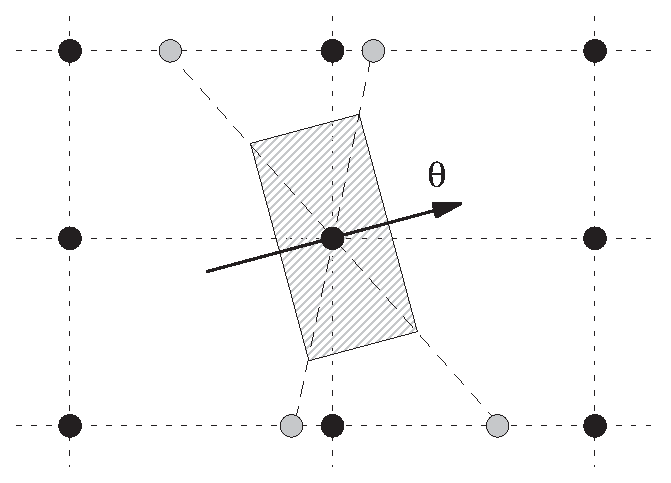
\epsfig{file=./GSE_1.eps,angle=0,width=2.2in}
\caption{Graphical depiction of spatial averaging GSE alleviation technique
used here. Solid circles and dotted lines represent the spatial grid. Hatched
area represent averaging area to be considered. Corner point values are
obtained from the central grid point and the gray points. The latter values
are obtained by interpolation from adjacent grid points
\citep[from][]{tol:OMOD02b}.}
\label{fig:GSE_1} \botline
\end{center}
\end{figure}

\noindent
where $\gamma_{a,s}$ and $\gamma_{a,n}$ are tunable constants, the default
value of which is set to 1.5. This averaging is graphically depicted in
Fig.~\ref{fig:GSE_1}. Note that these values may require some retuning for
practical applications, as discussed in \cite{tol:OMOD02b}. Appendix A of the
latter paper presents details of the averaging scheme, including conservation
considerations. Consistency with the \cite{art:BH87} approach furthermore
implies that $\gamma_{a,s}$ and $\gamma_{a,n}$ should vary with the spatial
grid resolution \citep[see][Appendix]{tol:OMOD08a}.

Note that this kind of averaging with dominant directions $\bs$ and $\bn$ is
similar to the \cite{art:BH87} diffusion method, that uses the same main
directions. The averaging method, however, never influences the time step,
because it is completely separated from the actual propagation. Moreover, if
explicit schemes are used with typically $c_g \Delta t / \Delta x < 1$, it is
obvious that the averaging over the area as defined in (\ref{eq:GSE_avg}) will
generally require information at directly neighboring spatial grid points
only, as in Fig.~\ref{fig:GSE_1}. Furthermore, this method does not require
high-latitude filtering.

As is illustrated in \cite{tol:OMOD02b,tol:OMB02b}, this method gives
virtually identical results as the previous method, but does so at slightly
lower costs. For high resolution applications, the averaging method may become
dramatically more economical.

A third possible GSE alleviation method considers that the advection for a
give discrete spectral bin is not unidirectional but divergent
\citep[see][]{tol:OMOD02b}.  An early version of this method was included in
model version 1.18. Because this method has not yet been developed to
maturity, it is not provided with the present release of \ws.

Finally, the GSE can be alleviated somewhat by assuring that the discrete
spectral directions do not coincide with spatial grid lines. This can be
achieved by defining the first discrete direction $\theta_1$ as

% eq:theta1          First direction

\begin{equation}
\theta_1 = \alpha_\theta \: \Delta \theta \:\:\: , \label{eq:theta1}
\end{equation}

\noindent
where $-0.5 \leq \alpha_\theta \leq 0.5$ can be defined by the user. Note that
setting $\alpha \neq 0$ is beneficial to the first order scheme, but has
negligible impact on the third order scheme.
 


% -------------------------------------------------------------
\vsssub
\subsubsection{~Unresolved obstacles} \label{sec_obst}
\vsssub

Even with the original tuning of \ws\ version 1.15 \citep{tol:OMB02a}, it was
clear that unresolved islands groups are a major source of local wave model
errors. This was illustrated in some more detail in
\citet[][Fig.~3]{tol:Waves01a}, and \citet[][Fig.~8]{tol:WaF02}. In \ws, a
methodology from the \swan\ model \citep{art:BRH99,man:SWAN3} was adopted to
apply the effects of unresolved obstacles at the cell boundaries of the
spatial grid within the numerical scheme. In this approach, the numerical
fluxes between cells through their common boundary are suppressed according to
the degree of obstruction provided by the unresolved obstacle. In this
approach, the numerical propagation scheme of the \uq\ scheme of
Eq.~(\ref{eq:uq_xy_tot}) is modified as

% eq:uq_xy_obstr

\begin{equation}
\cN_{i,j,l,m}^{n+1} = \cN_{i,j,l,m}^n +
\frac{\Delta t}{\Delta \phi} \left [ \alpha_{i,-} \cF_{i,-} - \alpha_{i,+} \cF_{i,+} \right ]
\: . \label{eq:uq_xy_obstr} \end{equation}

\noindent
where $\alpha_{i,-}$ and $\alpha_{i,+}$ are `transparencies' of the
corresponding cell boundaries, ranging from 0 (closed boundary) to 1 (no
obstructions). For outflow boundaries, transparencies by definition are 1,
otherwise energy will artificially accumulate in cells. For inflow boundaries,
transparencies less than 1 result in elimination of obstructed energy at the
cell boundary. This approach is graphically depicted in
Fig.~\ref{fig:obstr}. Note that a similar approach is easily adopted in the
first order scheme (\ref{eq:1up_xy_tot}). Note, furthermore, that an alternate
obstruction approach with obstructions as a function of the spectral direction
$\theta$ has been used by \cite{art:HY96} and \cite{art:HMM00}.

\begin{figure} \begin{center}
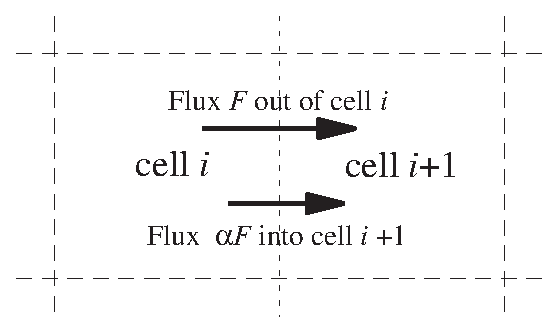
\epsfig{file=./obstr.eps,angle=0,width=2.2in}
\caption{Graphical depiction of treatment of unresolved obstacles. Common cell
         boundary (dotted line) has transparency $\alpha$. Dashed lines
         represent other cell boundaries. Numerical flux from left to right.}
         \label{fig:obstr} \botline
\end{center}
\end{figure}

Two methods for defining the obstructions are available in the model. The
first defines the obstructions directly at the grid boundary. This requires
the generation of staggered depth-transparency grids. The second allows the
user to define depths and transparencies at the same grid. In this case, the
transparency at the inflow boundary becomes $0.5(1+\alpha_i)$, and the outflow
transparency by definition is 1. To complete the total transparency
$\alpha_i$, the next cell in the flow direction will have an inflow
transparency $2\alpha_i/(1+\alpha_i)$. If consecutive cells are partially
obstructed, the product of individual transparencies is applied.

This approach can also be used to continuously model the effects of ice
coverage on wave propagation. This will be discussed in \para~\ref{sub:ice}.
Details of the sub-grid treatment of islands and ice can be found in
\cite{tol:OMOD03a}. A study of impacts of this approach in large scale wave
models is presented in \cite{tol:OMB02b,tol:OMOD03a}.

The default setting of \ws\ is not to include sub-grid modeling of
obstacles. Generating obstruction grids can be labor intensive. For this
reason, an automated approach for generating bottom and obstruction grids was
developed by \cite{tol:MMAB07a, tol:OMOD08a}.  Note that this option does not
involve compile-level choices, but is entirely controlled from the grid
preprocessor (see following chapter).


% -------------------------------------------------------------
\vsssub
\subsubsection{~Shoreline reflection \hfill {\rm (F. Ardhuin)}} \label{sec_refl}
\vsssub
In the case of  icebergs and subgrid islands, the reflected energy is redistributed evenly in all directions within 90$^\circ$ of the direction opposite to 
the incoming waves. 
For resolved lands,  a mean direction perpendicular to shore $\theta_n$ was defined 
from the land or sea status of the 8 grid points surrounding the local point (Fig. \ref{fig:refl}). 

For each model grid point adjacent to land, the analysis of the land-sea geometry gives one value of $\theta_n$  among
16 possible directions. Together with any incoming wave direction $\theta_i$ this defines a specular reflection direction $\theta_r=2 \theta_n - \theta_i + \pi$.  
For each spectral component of direction $\theta_i$ going towards the coast (i.e. such that $\cos(\theta_i-\theta_n) >0$),  the total reflection 
is $R^2$ times the incoming  energy. This reflected energy $R^2 E(f) M(f,\theta_i)$ is redistributed over directions 
around the specular reflection direction $\theta_r$, with a broad distribution taken proportional to $\cos^n(\theta-\theta_r)$, where the power $n$ 
is a function of the local shoreline geometry. 

\begin{figure} \begin{center}
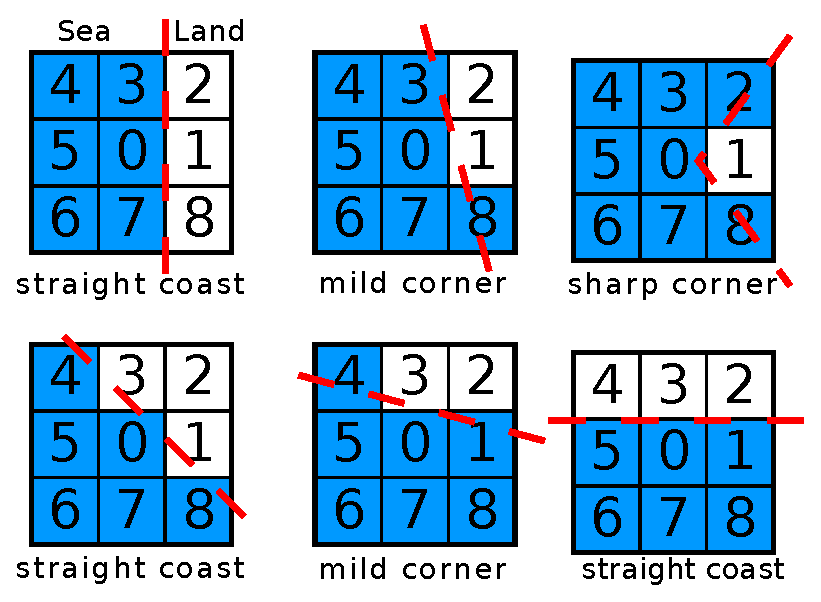
\epsfig{file=./coast_reflection.eps,angle=0,width=3in}
\caption{Examples of determination of the shoreline orientation and geometry using the land / sea mask. For any sea point (number 0) which is the ocean (in blue) 
and has at least one neighbor in land (in white) the eight neighbors, numbered from 1 to 8 are used to define the shoreline geometry. 
For `mild' corners and straight coasts, the estimated shoreline orientation (dashed line) is used to compute the directional distribution of the reflected wave energy.  
}
\label{fig:refl} \botline
\end{center}
\end{figure}

For this purpose we distinguish three different shoreline geometries relative to the local point as illustrated by 
figure \ref{fig:refl}: we set  $n=2$ for a straight coast (three connected land points 
among the neighbors), $n=1$ for a mild corner (two land points 
among the neighbors), and $n=0$ at a sharp corner (only one land point, among the 4 closest neighbors) which corresponds to the 
same treatment done for subgrid islands and icebergs. Changing these values of $n$ in the range $0$ to $2$  has little effects on our results. 
$n=1$ corresponds to a Lambertian surface approximation, which is used for electromagnetic wave scattering from rough surfaces. A pure 
specular reflection would be obtained with $n$ infinite. 
A more rigorous 
treatment should use the distribution of the shoreline orientation at at the scale of the ocean wavelength, namely of the order of 100~m. 

% -------------------------------------------------------------
\vsssub
\subsubsection{~Propagation on curvilinear grids \hfill {\rm (Rogers and Campbell)}} \label{sec_irreg}
\vsssub

Computations may be made on curvilinear grids within \ws\ . This makes it possible to run the model on alternate grid projections 
(e.g. Lambert conformal conic), rotated grids, or shoreline-following grids with higher resolution near shore, though the 
restrictions on time step from the conditionally stable schemes still apply. The same propagation schemes are utilized for 
irregular grids as for regular grids (first order upwind explicit or ULTIMATE QUICKEST).

Regarding the method: the implementation is described in \citep{RogCamp:NRLrep09}, summarized here: a Jacobian is used to convert 
the entire domain between the normal, curving space, and a straightened space. This conversion is performed only within the 
propagation routine, rather than integrating the entired model in straightened space. A simple, three step process is used every 
time the propagation subroutine is call (i.e. every time step and every spectral component): first, the dependent variable 
(wave action density) is converted to straightened space using a Jacobian; second, the wave action density is propagated via 
subroutine calls for each (of two) grid axes; third, the wave action density is converted back to normal, curved space. The actual 
flux computation is not significantly modified from its original, regular grid form. The same process occurs, regardless of grid 
type (regular or irregular); for regular grids, the Jacobian is unity.

Regarding the user interface: in {\file ww3\_grid.inp}, a string is used to indicate the grid type. In cases where this grid 
string is `{\F RECT}', the model processes input for a regular grid. In case where this grid string is `{\F CURV}' , the model 
processes input for an irregular grid. [Note that with \ws\ version 4.00, the coordinate system (i.e. degrees vs. meters) and 
the closure type (e.g. global/wrapping grid) are also specified in  {\file ww3\_grid.inp} ; the switches LLG and XYG are deprecated.] 

% -------------------------------------------------------------
\vsssub
\subsubsection{~Use of triangle-based unstructured grids \hfill {\rm (Roland and Ardhuin)}} \label{sec_prug}
\vsssub
Triangle-based grids can be used in \ws\ with numerical schemes based on contour residual distribution \citep[][for a review]{PhD:Rol}. 
This option is activated by setting the  grid string to `{\F UNST}' in {\file ww3\_grid.inp}.
Four schemes have been implemented, and the choice of one or the other is done with the UG namelist. 
These are the N scheme, the PSI scheme, the FCT scheme, and one implicit scheme. The default is the faster but more diffusive N scheme. 

In practice the grid can be easily generated, using the Polymesh interface (software developed by T.U. Darmstadt), 
from a shoreline polygons database \citep[e.g.][]{art:WS96} and a list of depth soundings, regular
or irregular. 

Regarding the method: the evolution of the spectrum at the nodes, where it is evaluated, is based on the redistribution over the nodes of
the flux convergence into the median dual cells associated with the nodes (see figure \ref{fig:triangles}).
\begin{figure} \begin{center}
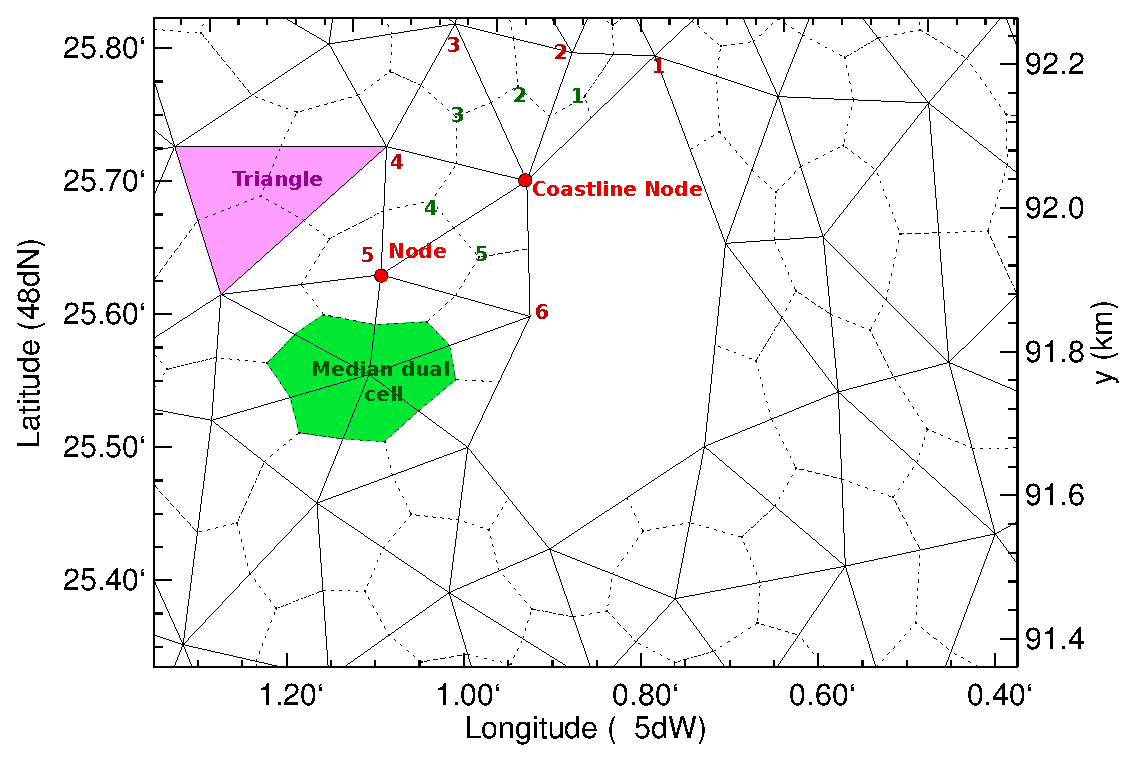
\epsfig{file=./grid_triangles.eps,angle=0,width=6in}
\caption{Example of a region of a triangle-based mesh, with in this case the small Island of Bannec, France. If the depth is greater than 
the minimum depth, the nodes of the shoreline are active. These are characterized by a larger number of neighbor nodes (6 in the example chosen) 
than neighbor triangles (5 in the same example). 
}
\label{fig:triangles} \botline
\end{center}
\end{figure}
 For any  spectral component, the advection equation (\ref{eq:step_xy_prop}) is solved on the median dwell cells: the incoming flux into a
cell gives the rate of change of the wave action at the corresponding node. The various schemes implemented have 
different discretizations for the estimation of this flux. 

 The boundary condition at the shoreline depends on the 
wave direction relative to the shoreline orientation. This particular treatment is enforced using the `{\F IOBPD}' array 
which is updated whenever the grid points status map `{\F MAPSTA}' changes. The grid geometry is also used to define 
local gradients of the water depth and currents. All other operations, such as interpolation of the forcing 
on the grid and interpolation from the grid onto output locations, is performed using linear interpolation in triangles. 

All the triangle geometry operations assume a locally flat Earth. 



% -------------------------------------------------------------
\vssub
\subsection{~Intra-spectral propagation}
\vssub

The third step of the numerical algorithm considers refraction and residual
(current-induced) wavenumber shifts. For both the spherical and Cartesian
grid, the equation to be solved in this step becomes

%-----------------------------------%
% Step : Intra-spectral propagation %
%-----------------------------------%
% eq:step_intra
% eq:k_dot_g

\begin{equation}
\frac{\p N}{\p t} + \frac{\p}{\p k} \, \dot{k}_g N +
\frac{\p}{\p \theta} \, \dot{\theta}_g N = 0
\: , \label{eq:step_intra} \end{equation} \begin{equation}
\dot{k}_g  = \frac{\p \sigma}{\p d} 
    \frac{{\bf U} \cdot \nabla_x d}{c_g}  -
    {\bf k} \cdot \frac{\p {\bf U}}{\p s}
\: . \label{eq:k_dot_g} \end{equation}

\noindent
where $\dot{k}_g$ is the wavenumber velocity relative to the grid, and
$\dot{\theta}_g$ is given by (\ref{eq:theta_g_dot}) and (\ref{eq:theta_dot}).
This equation does not require boundary conditions in $\theta$-space, as the
model by definition uses the full (closed) directional space. In $k$-space,
however, boundary conditions are required. At low wavenumbers, it is assumed
that no wave action exists outside the discrete domain. It is therefore
assumed that no action enters the model at the discrete low-wavenumber
boundary. At the high-wavenumber boundary, transport across the discrete
boundary is calculated assuming a parametric spectral shape as given by
Eq. (\ref{eq:tail_N_k}). The derivatives of the depth as needed in the
evaluation of $\dot{\theta}$ are mostly determined using central
differences. For points next to land, however, one-sided differences using sea
points only are used.

Propagation in $\theta$-space can cause practical problems in an explicit
numerical scheme, as the refraction velocity can become extreme for long waves
in extremely shallow water or due to strong current shears. Similarly, 
the propagation in $k$-space suffers from similar problems in very shallow water. 
To avoid the need of extremely small time steps
due to refraction, the propagation velocities in $\theta$-space and $k$-space
(\ref{eq:theta_dot}) are filtered,

% eq:theta_filter

\begin{equation}
\dot{\theta} = X_{rd}(\lambda,\phi,k)\left( \dot{\theta_d} + 
\dot{\theta_c} + \dot{\theta_g} \right)\: , \label{eq:theta_filter} \end{equation}

\noindent
where the indices d, c and g refer to the depth, current and great-circle related fraction of
the refraction velocity in (\ref{eq:theta_dot}). The filter factor $X_{rd}$ is
calculated for every wavenumber and location separately, and is determined so
that the \cfl\ number for propagation in $\theta$-space due to the {\em depth}
refraction term cannot exceed a pre-set (user defined) value (default
0.7). This corresponds to a reduction of the bottom slope for some low
frequency wave components. For mid-latitudes, the effected components are expected to carry
little energy because they are in extremely shallow water. Long wave
components carrying significant energy are usually traveling toward the coast,
where their energy is dissipated anyway. This filtering is also important for short waves, 
and close to the pole. The effect of this filter can be tested by reducing the time steps for
intraspectral refraction and by looking at the maximum CFL numbers in the output of the model. 
These are computed just before the filter is applied. 

\vspace{\baselineskip} \noindent 
As with the propagation in physical space, a first order and an \uq\ scheme
are available. In the first order scheme the fluxes in $\theta$- and $k$-space
are calculated Cf. Eqs. (\ref{eq:1up_xy_1}) through (\ref{eq:1up_xy_3})
(replacing $\cN$ with $N$ and rotating the appropriate counters). The complete
first order scheme becomes

% eq:1up_intra_tot

\begin{equation}
N_{i,j,l,m}^{n+1} = N_{i,j,l,m}^n 
 + \frac{\Delta t}{\Delta \theta} \left [ \cF_{l,-} - \cF_{l,+} \right ]
 + \frac{\Delta t}{\Delta k_m} \left [ \cF_{m,-} - \cF_{m,+} \right ]
\: , \label{eq:1up_intra_tot} \end{equation}

\noindent
where $\Delta \phi$ is the directional increment, and $\Delta k_m$ is the
(local) wavenumber increment. The low-wavenumber boundary conditions is
applied by taking $\cF_{m,-}=0$ for $m=1$, and the high wavenumber boundary
condition is calculated using the parametric approximation (\ref{eq:tail_N_k})
for N, extending the discrete grid by one grid point to high wavenumbers.

\vspace{\baselineskip} \noindent
The \uq\ scheme for the $\theta$-space is implemented similar to the scheme
for physical space, with the exception that the closed direction space does
not require boundary conditions. The variable grid spacing in $k$-space
requires some modifications to the scheme as outlined by
\cite[{Appendix}]{art:Leo79}. Equations~(\ref{eq:quick_1}) through
(\ref{eq:quick_4}) then become

% ------ QUICKEST scheme for k space---------- %
% eq:quick_1k        Basic flux
% eq:quick_2k        Boundary value
% eq:quick_3k        Divergence
% eq:quick_4k        CFL number

\begin{equation}
\cF_{m,-} = \left [ \dot{k}_{g,b} \: N_b \: \right ]^n_{i,j,l}
\: , \label{eq:quick_1k}\end{equation} \begin{equation}
\dot{k}_{g,b} = 0.5 \: \left ( \dot{k}_{g,m-1} + \dot{k}_{g,m} 
\: \right )  \: , \label{eq:quick_1ak}
\end{equation} \begin{equation}
N_b = \frac{1}{2} \left [ \rule[0mm]{0mm}{\baselineskip} \: 
(1+C)N_{i-1} + (1-C)N_i \: \right ] - \:
\frac{1-C^2}{6} \: {\cal CU} \: \Delta k^2_{m-1/2}, \label{eq:quick_2k} \end{equation} \begin{equation}
{\cal CU} =  \left \{ \begin{array}{ccc}
\frac{1}{\Delta k_{m-1}}
\left [ \frac{N_{ m }-N_{m-1}}{\Delta k_{m-1/2}} - 
        \frac{N_{m-1}-N_{m-2}}{\Delta k_{m,-3/2}} \right ]
               & \mbox{for} & \dot{k}_b \geq 0 \\
\frac{1}{\Delta k_m}
\left [ \frac{N_{m+1}-N_{ m }}{\Delta k_{m+1/2}} -
       \frac{N_{ m }-N_{m-1}}{\Delta k_{m-1/2}} \right ]
               & \mbox{for} & \dot{k}_b   <  0
\end{array} \right . \: , \label{eq:quick_3k}
\end{equation} \begin{equation}
C = \frac{\dot{k}_{g,b} \: \Delta t}{\Delta k_{m-1/2}}
\: , \label{eq:quick_4k} \end{equation}

\noindent
where $\Delta k_m$ is the discrete band or cell width at grid point $m$, and
where $\Delta k_{m-1/2}$ is the distance between grid points with counters $m$
and $m-1$. The \ult\ limiter can be applied as in Eqs.~(\ref{eq:ult_1})
through (\ref{eq:ult_4}), if the \cfl\ number of Eq.~(\ref{eq:quick_4k}) is
used. At the low- and high-wavenumber boundaries the fluxes again are
estimated using a first-order upwind approach, with boundary conditions as
above defined for the first-order scheme. The final scheme in $k$-space
becomes

% eq:1uq_k_tot

\begin{equation}
N_{i,j,l,m}^{n+1} = N_{i,j,l,m}^n 
 + \frac{\Delta t}{\Delta k_m} \left [ \cF_{m,-} - \cF_{m,+} \right ]
\: , \label{eq:uq_k_tot} \end{equation}


% -------------------------------------------------------------
\vssub
\subsection{~Source terms} \label{sub:source}
\vssub

Finally, the source terms are accounted for by solving

%---------------------%
% Step : Source terms %
%---------------------%
% eq:step_source

\begin{equation}
\frac{\p N}{\p t} = \cS \: . \label{eq:step_source}
\end{equation}

\noindent 
As in \wam, a semi-implicit integration scheme is used. In this scheme the
discrete change of action density $\Delta N$ becomes \citep{art:WAM88}

% eq:implicit_st

\begin{equation}
\Delta N(k,\theta) = \frac{\cS(k,\theta)}{1- \epsilon D(k,\theta)\Delta t}
\: , \label{eq:implicit_st} \end{equation}

\noindent 
where $D$ represents the diagonal terms of the derivative of $\cS$ with
respect to $N$ \citep[Eqs. 4.1 through 4.10]{art:WAM88}, and where $\epsilon$
defines the offset of the scheme. Originally, $\epsilon = 0.5$ was implemented
to obtain a second order accurate scheme. Presently, $\epsilon = 1$ is used as
it is more appropriate for the large time steps in the equilibrium range of
the spectrum \citep{pro:HA98,art:HA01}, and as it result in much smoother
integration of the spectrum. The change of $\epsilon$ has little impact on
mean wave parameters, but makes the dynamical time stepping as described below
more economical.

The semi-implicit scheme is applied in the framework of a dynamic
time-stepping scheme \citep{tol:JPO92}. In this scheme, integration over the
global time step $\Delta t_g$ can be performed in several dynamic time steps
$\Delta t_d$, depending on the net source term $\cS$, a maximum change of
action density $\Delta N_m$ and the remaining time in the interval $\Delta
t_g$. For the $n^{\rm th}$ dynamic time step in the integration over the
interval $\Delta t_g$, $\Delta t_d^n$ is calculated in three steps as

% ------ Dynamic s.t. int. scheme ------- %
% eq:st_d_1
% eq:st_d_2a
% eq:st_d_2b
% eq:st_d_3

\begin{equation}
\Delta t_d^n = 
\min_{f<f_{hf}} \left [ \frac{\Delta N_m}{|\cS|}
\left ( 1 + \epsilon D \frac{\Delta N_m}{|\cS|} \right ) ^{-1}
\right ] \: , \label{eq:st_d_1}
\end{equation} \begin{equation}
\Delta t_d^n = \max \: \left [ \: \Delta t_d^n \: , \: 
\Delta t_{d,\min} \right ] \: , \label{eq:st_d_2a}
\end{equation} \begin{equation}
\Delta t_d^n = \min \: \left [ \: \Delta t_d^n \: , \: 
\Delta t_g - \sum_{i=1}^{n-1} \Delta t_d^i
 \: \right ] \: , \label{eq:st_d_2b}
\end{equation}

\noindent
where $\Delta t_{\min}$ is a user-defined minimum time step, which is added to
avoid excessively small time steps. The corresponding new spectrum $N^n$
becomes

\begin{equation}
N^n = \max\: \left [ \: 0 \: , \: N^{n-1} + 
\left ( \frac{\cS \Delta t_d}{1 - \epsilon D \Delta t_d} \right )
\: \right ] \: . \label{eq:st_d_3}
\end{equation}

\noindent 
The maximum change of action density $\Delta N_m$ is determined from a
parametric change of action density $\Delta N_p$ and a filtered relative
change $\Delta N_r$

% eq:st_d_4
% eq:st_d_5
% eq:st_d_6
% eq:st_d_7

\begin{equation}
\Delta N_m (k,\theta) = \min \: \left [ \:
\Delta N_p (k,\theta) \: , \: \Delta N_r (k,\theta) 
\: \right ] \: , \label{eq:st_d_4}
\end{equation} \begin{equation}
\Delta N_p (k,\theta) = X_p \: \frac{\alpha}{\pi} \:
\frac{(2\pi)^4}{g^2} \: \frac{1}{\sigma k^3}
\: , \label{eq:st_d_5}
\end{equation} \begin{equation}
\Delta N_r (k,\theta) = X_r \; \max \: \left [ \: 
N(k,\theta) \: , \: N_f \: \right ] \: , \label{eq:st_d_6}
\end{equation} \begin{equation}
N_f = \max \: \left [ \: \Delta N_p (k_{\max},\theta) \: , 
\: X_f \: \max_{\forall k,\theta} \left \{ N(k,\theta) \right \}
\: \right ] \: , \label{eq:st_d_7} \end{equation}

\noindent 
where $X_p$, $X_r$ and $X_f$ are user-defined constants (see
Table~\ref{tab:st_d_p}), $\alpha$ is a {\sc pm} energy level (set to $\alpha =
0.62\,10^{-4}$) and $k_{\max}$ is the maximum discrete wavenumber. The
parametric spectral shape in (\ref{eq:st_d_5}) corresponds in deep water to
the well-known high-frequency shape of the one-dimensional frequency spectrum
$F(f) \propto f^{-5}$. The link between the filter level and the maximum
parametric change in (\ref{eq:st_d_7}) is used to assure that the dynamic time
step remains reasonably large in cases with extremely small wave energies. A
final safeguard for stability of integration is provided by limiting the
discrete change of action density to the maximum parametric change
(\ref{eq:st_d_5}) in conditions where Eq.~(\ref{eq:st_d_2a}) dictates $\Delta
t_d^n$. In this case Eq.~(\ref{eq:st_d_2a}) becomes a limiter as in the WAM
model. Impacts of limiters are discussed in detail in for instance
\cite{art:HJ99,art:HJ01}, \cite{art:HA01} and \cite{tol:GAOS02}.

% tab:st_d_p

\begin{table} 
\begin{center} \begin{tabular}{|l|c|c|c|c|} \hline \hline
                 & $X_p$     & $X_r$             & $X_f$ &
$\Delta t_{d,\min}$      \\ \hline
\wam\ equivalent & $\frac{\pi}{24}10^{-3}\Delta t$
 & $\infty (\geq 1)$ & --    & $\Delta t_g$  \\ 
 suggested       & 0.1-0.2  & 0.1-0.2 & 0.05 & $\approx 0.1 \Delta t_g$ \\  
default setting  &  0.15    &   0.10  & 0.05 & -- \\ \hline \hline
\end{tabular} \end{center}
\caption{User-defined parameters in the source term integration
 scheme}
\label{tab:st_d_p} \botline \end{table}

The dynamic time step is calculated for each grid point separately, adding
additional computational effort only for grid points in which the spectrum is
subject to rapid change. The source terms are re-calculated for every dynamic
time step.

It is possible to compile \ws\ without using a linear growth term. In such a
case, waves can only grow if some energy is present in the spectrum. In
small-scale applications with persistent low wind speeds, wave energy might
disappear completely from part of the model. To assure that wave growth can
occur when the wind increases, a so-called seeding option is available in \ws\
(selected during compilation). If the seeding option is selected, the energy
level at the seeding frequency $\sigma_{\rm seed} = \min(\sigma_{\max}, 2\pi
f_{hf})$ is required to at least contain a minimum action density

% ------ Spectral seeding ------- %
% eq:seed

\begin{eqnarray}
N_{\min}(k_{seed},\theta) & = & 
        6.25 \: 10^{-4} \frac{1}{k_{\rm seed}^3 \: \sigma_{\rm seed}}
        \max \left [ \: 0. \: , \: \cos^2 ( \theta - \theta_w ) \right ]
                             \nonumber \\ & & \hspace{5mm}
        \min \left [ \: 1 \: , \: \max \left ( \: 0 \: , \: 
        \frac{|u_{10}|}{X_{\rm seed} g \sigma_{\rm seed}^{-1}}-1 
\: \right ) \: \right ] \: , \label{eq:seed} \end{eqnarray}

\noindent
where $g \sigma_{\rm seed}^{-1}$ approximates the equilibrium wind speed for
the highest discrete spectral frequency. This minimum action distribution is
aligned with the wind direction, goes to zero for low wind speeds, and is
proportional to the integration limiter (\ref{eq:st_d_5}) for large wind
speeds. $X_{\rm seed} \geq 1$ is a user-defined parameter to shift seeding to
higher frequencies. Seeding starts if the wind speed reaches $X_{\rm seed}$
times the equilibrium wind speed for the highest discrete frequency, and
reaches its full strength for twice as high wind speeds. The default model
settings include the seeding algorithm, with $X_{\rm seed} = 1$.

In model version 3.11, surf-zone physics parameterizations have been
introduced. Such physics, particularly depth-induced breaking, operate on much
smaller time scales than deep water and limited depth physics outside the surf
zone. To assure reasonable behavior for larger time steps, an additional
optional limiter has been adopted from the SWAN model, similar to the Miche
style maximum wave height in the depth limited wave breaking source term of
Eq.~(\ref{eq:BJ78_Miche}). In this limiter, the maximum wave energy $E_m$ is
computed as

% ------ Surf zone limiter ------ %
% eq:MLIM

\begin{equation}
E_m = \frac{1}{16} [ \gamma_{lim} \:\bar{k} \: \tanh ( \bar{k} d ) ] ^2
\:\:\: , \label{eq:MLIM} 
\end{equation}

\noindent
where $\gamma_{lim}$ is a factor comparable to $\gamma_M$ in
Eq.~(\ref{eq:BJ78_Miche}), with the caveat that $\gamma_M$ is representative
for an individual wave, whereas $\gamma_{lim}$ is representative for the
significant wave height. If the total spectral energy $E$ is larger than the
maximum energy $E_m$, the limiter is applied by simply rescaling the spectrum
by the factor $E/E_m$, loosely following the argumentation from
\cite{art:EB96} ad used in \para\ref{sec:BJ}. 

This limiter can be switch on or off in the compilation of the model, and
$\gamma_{lim}$ can be adjusted by the user (default $\gamma_{lim} =
0.75$). Note that this limiter should be used as a `safety valve' only, and
hence that it should be less strict than the breaking criterion in the
surf-breaking source term, if this source term is modeled explicitly.


\pb
% -------------------------------------------------------------
\vssub
\subsection{~Winds and currents}
\vssub

\noindent
Model input mainly consists of wind and current fields. Within the model,
winds and currents are updated at every time step $\Delta t_g$ and represent
values at the end of the time step considered. Several interpolation methods
are available (selected during compilation). By default, the interpolation in
time consists of a linear interpolation of the velocity and the direction
(turning the wind or current over the smallest angle). The wind speed or
current velocity can optionally be corrected to (approximately) conserve the
energy instead of the wind velocity. The corresponding correction factor $X_u$
is calculated as

% eq:X_u10

\begin{equation}
X_u = \max \left [ \: 1.25 \: , \: \frac{u_{10,rms}}{u_{10,l}}
\right ] \: , \label{eq:X_u10} \end{equation}

\noindent
where $u_{10,l}$ is the linearly interpolated velocity and $u_{10,rms}$ is the
rms interpolated velocity. Finally, winds can optionally be kept constant and
changed discontinuously (option not available for current).

\vspace{\baselineskip} \noindent 
Note that the auxiliary programs of \ws\ include a program to pre-process
input fields (see \para\ref{sec:prep}). This program transfers gridded fields
to the grid of the wave model. For winds and currents this program utilizes a
bilinear interpolation of vector components. This interpolation can be
corrected to (approximately) conserve the velocity or the energy of the wind
or the current by utilizing a correction factor similar to
Eq.~(\ref{eq:X_u10}).


\pb
% -------------------------------------------------------------
\vssub
\subsection{~Use of tidal analysis \hfill {\rm (F. Ardhuin)}}
\vssub

\noindent
In order to reduce the volume of input files, the water levels and currents 
can be defined by their tidal amplitudes and phases. This is made possible 
by using the 'TIDE' switch which activates the detection of the needed 
information in current.ww3 
and level.ww3 files. The tidal analysis can be performed from NetCDF current 
or water level files, using the ww3\_prnc preprocessing program. In that case 
the analysis method uses the flexible tide analysis package by \cite{art:For09}. 
At present the choice of tidal constituents is hard coded to 20, namely, 
Z0 (mean), SSA, MSM, MSF, MF, 2N2, MU2, N2, NU2, M2, S2, K2, MSN2, MN4, M4, MS4, S4,
M6, 2MS6, and  M8. Another arbitrary choice is the time step at which currents or water 
level will be updated. This is now set to 1800~s. We also note that in the present 
version, this definition of currents and water levels can only be used with single grids, 
when using ww3\_shel. 

Memory usage and time of analysis can be greatly reduced by removing some usually negligible constituents, 
such as MSM, SSA,  MSM, 2N2, or even M8. 


% -------------------------------------------------------------
\vssub
\subsection{~Ice coverage} \label{sub:ice}
\vssub

\noindent
Ice covered sea is considered as `land' in \ws, assuming zero wave energy and
boundary conditions at ice edges are identical to boundary conditions at shore
lines. Grid points are taken out of the calculation if the ice concentration
becomes larger than a user-defined concentration. If the ice concentration
drops below its critical value, the corresponding grid point is
`re-activated'. The spectrum is then initialized with a PM spectrum based on
the local wind direction with a peak frequency corresponding to the
second-highest discrete frequency in the grid. A small spectrum is used to
assure that spectra are realistic, even for shallow coastal points.

The above discontinuous ice treatment represents the default model setting in
\ws. In the framework of the modeling of unresolved obstacles as discussed in
\para\ref{sec_obst}, a continuous method is also available, as given by
\cite{tol:OMOD03a}. In this method, a user-defined critical ice concentration
at which obstruction begins ($\epsilon_{c,0}$) and is complete
($\epsilon_{c,n}$) are given (defaults are $\epsilon_{c,0} = \epsilon_{c,n} =
0.5$, i.e., discontinuous treatment of ice). From these critical
concentrations, corresponding decay length scales are calculated as,

\begin{equation}
l_0 = \epsilon_{c,0} \min ( \Delta x , \Delta y )
\:\:\: . \label{eq:l0}
\end{equation}
\begin{equation}
l_n = \epsilon_{c,n} \min ( \Delta x , \Delta y )
\:\:\: . \label{eq:ln}
\end{equation}

\noindent
from which cell transparencies in $x$ and $y$ ($\alpha_x$ and $\alpha_y$,
respectively) are calculated as

\begin{equation}
\alpha_x = \left \{ \begin{array}{ccl}
 1 & \mbox{for} & \epsilon \Delta x < l_0 \\
 0 & \mbox{for} & \epsilon \Delta x > l_n \\
\frac{l_n - \epsilon \Delta x}{l_n - l_0} & \multicolumn{2}{c}{\mbox{otherwise}} 
\end{array} \right .
\:\:\: , \:\:\:
\alpha_y = \left \{ \begin{array}{ccl}
 1 & \mbox{for} & \epsilon \Delta y < l_0 \\
 0 & \mbox{for} & \epsilon \Delta y > l_n \\
\frac{l_n - \epsilon \Delta y}{l_n - l_0} & \multicolumn{2}{c}{\mbox{otherwise}} 
\end{array} \right .
\:\:\: . \label{eq:ice_0} 
\end{equation}

\noindent
Details of this model can be found in \cite{tol:OMOD03a}.

Updating of the ice map within the model takes place at the discrete model
time approximately half way in between the valid times of the old and new ice
maps. The map will not be updated, if the time stamps of both ice fields are
identical.


% -------------------------------------------------------------
\vssub
\subsection{~Spectral partitioning \hfill {\rm (B. Tracy)}}
\vssub

Figure \ref{fig:partitions} shows an example surface plot of an energy density
spectrum at one grid point at a specific time.  The amount of energy density
at each frequency-direction intersection is shown by this surface.  The
surface is divided into shaded areas or partitions representing energy from
sub-peaks within the spectrum.  Figure \ref{fig:partitions} shows four
spectral partitions, an area of windsea and three swell trains.  The total
energy represented by this spectrum can be defined by bulk parameters, such as
the significant wave height $H_s$. The shaded areas, called partitions of the
spectrum, show spectral sub-features that give more information about this
grid point's energy situation.  \ws\ has point and field output options
available to provide quantitative descriptions of these individual spectral
partition such as partition wave height, peak period of partition (parabolic
fit), peak wavelength of partition, mean direction of partition, wind-sea
fraction of partition ($W$) using Eq.~(\ref{eq:wsf}), and the number of
partitions.  In the field output, these parameters correspond to output fields
\ref{out:first_part} through \ref{out:last_part} and can be found in
\para\ref{sub:outpars}.

\begin{figure} \begin{center}
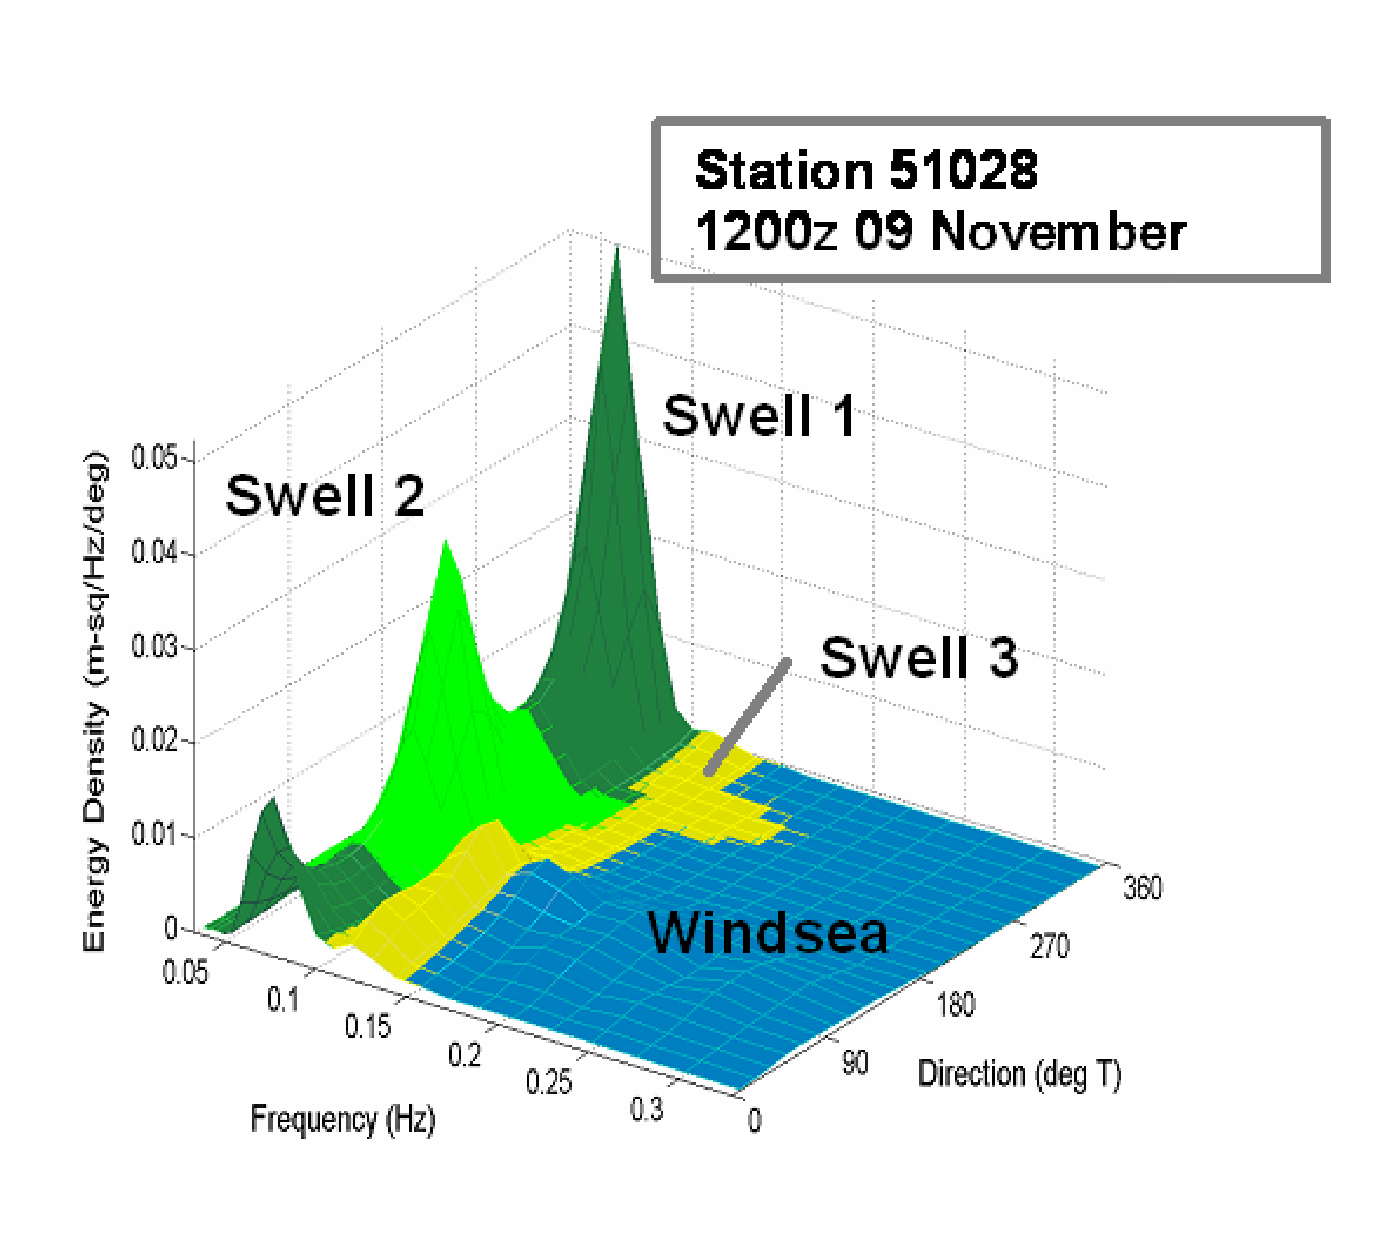
\epsfig{file=./partition.eps,width=4.0in}
\caption{Surface plot of an energy density spectrum showing spectral
         partitions for windsea and three swell trains.  This is a snapshot of
         hindcasted conditions at Christmas Island (NOAA buoy 51028) at
         12:00~UTC on November 9, 2000..}
         \label{fig:partitions} \botline
\end{center}
\end{figure}

Since the two-dimensional spectrum in Fig.~\ref{fig:partitions} looks like a
topological surface, it is logical to apply an image processing partitioning
algorithm that treats the spectral surface like a topographical surface.  The
partitioning shown in Fig.~\ref{fig:partitions} is based on a digital image
processing watershed algorithm \citep{art:VS91} first prototyped by
\cite{pro:HJ04} for the analysis of ocean wave data. The continental divide
where everything to the east goes into the Atlantic Ocean and everything to
the west goes into the Pacific Ocean is a typical example of a watershed line.
The oceans represent minima that determine the watershed line.  If the
spectral surface is inverted, the spectral peaks become catchments and
watershed lines or partition boundaries can be determined using the
\cite{art:VS91} algorithm.  Calculation of parameters for each spectral
partition can then be accomplished and wave system analysis as described in
\cite{art:HP01} can be applied.  \cite{pro:HJ04} and \cite{tol:Vict06b} used a
MATLAB code to apply the \cite{art:VS91} algorithm\footnote{~Now available as
XWaves from http://www.WaveForceTechnologies.com, replacing the previous APL
WAVES package}.  This code has been transformed to an efficient FORTRAN
routine for use in the version 3.11 of \ws.  Coding follows the
\cite{art:VS91} paper but incorporates an efficient sort routine (O(n))
discussed in \cite{rep:TTH06}.


% -------------------------------------------------------------
\vssub
\subsection{~Spatial and temporal tracking of wave systems 
\hfill {\rm (Van der Westhuysen, Hanson and Devaliere)}}
\vssub

The spectral partitioning procedure described above is carried out within 
the spectral space, independently at each geographical grid point. As a 
result, there is no coherence between the identified partitions over 
geographical space and in time. Following \cite{art:VMH97}, \cite{art:HP01} 
and \cite{pro:DHL09}, a spatial correlation step is therefore applied. 
This is done by means of an outwardly running spiral, originating at an 
arbitrary point (typically the center) inside the computational domain. 
Figure~\ref{fig:wavetrack} presents an example of such a tracking spiral on a regular 
computational grid over a coastal domain featuring landmass. At the spiral 
origin (location~1), each spectral partition is assigned an initial system 
index. The spatial correlation is then determined for each subsequent 
geographical location (2, 3, 4, ...) moving outward along the spiral. 
At each new geographical location, the peak period $T_\mathrm{p}$, peak 
direction $\theta_\mathrm{p}$ and significant wave height $H_\mathrm{m0}$ 
of each of its spectral partitions are correlated with the spatial means 
$\tilde{T}^\mathrm{n}_{\mathrm{p},i}$, $\tilde{\theta}^\mathrm{n}_{\mathrm{p},i}$ 
and $\tilde{H}^\mathrm{n}_{\mathrm{m0},i}$ of the corresponding parameters 
at its neighboring geographical grid points (indicated by the superscript 
$\mathrm{n}$) previously assigned a system $i$. the partition at the present 
grid point is assigned to the neighboring system $i$ that minimizes the 
following Goodness-of-Fit (GoF) function:

\begin{figure} \begin{center}
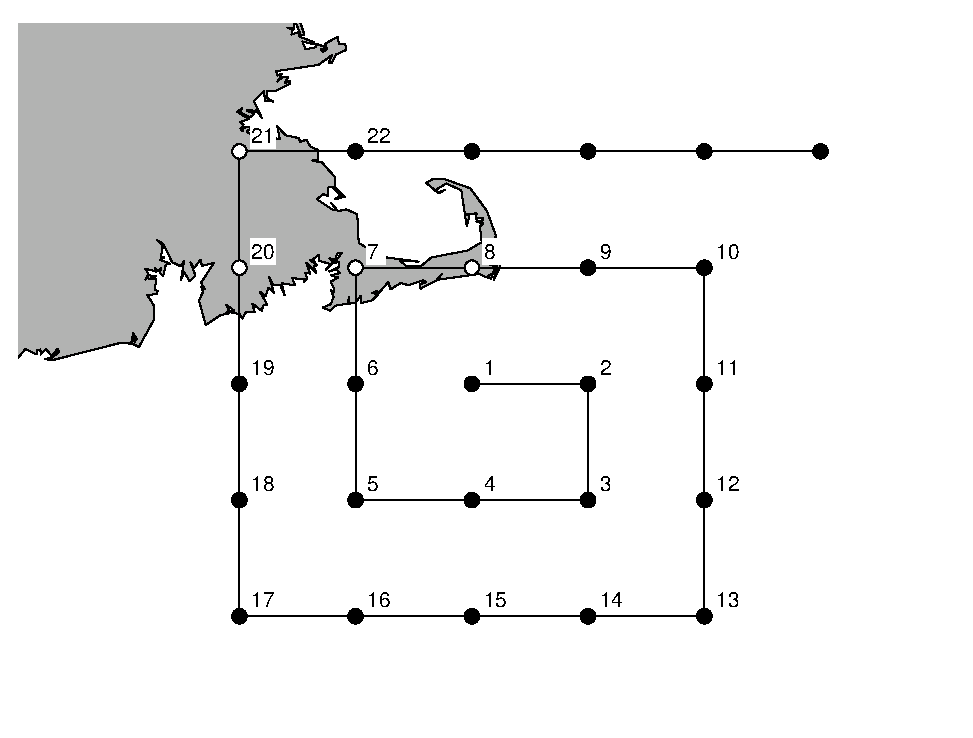
\epsfig{file=./wavetrack.eps,width=5.0in}
\caption{Example of a tracking spiral on a regular computational grid 
over a coastal domain featuring landmass (shaded). Black dots indicate 
active grid points and white dots indicate inactive (dry) grid points.}
         \label{fig:wavetrack} \botline
\end{center}
\end{figure}

\begin{equation}
    GoF_{i} = {\left( \frac{T_\mathrm{p} - \tilde{T}^\mathrm{n}_{\mathrm{p},i}}{\Delta T_\mathrm{n}} \right)}^2 + 
                     {\left( \frac{\theta_\mathrm{p} - \tilde{\theta}^\mathrm{n}_{\mathrm{p},i}}{\Delta\theta_\mathrm{n}} \right)}^2 +
                     {\left( \frac{H_\mathrm{m0} - \tilde{H}^\mathrm{n}_{\mathrm{m0},i}}{\Delta H_\mathrm{n}} \right)}^2\ \ ,
\label{eq:grdgof}
\end{equation} 

where $\Delta T_\mathrm{n}$, $\Delta\theta_\mathrm{n}$ and $\Delta H_\mathrm{n}$ 
are combining criteria, see \cite{art:WHD13}. If either of 
the first two terms on the RHS of (\ref{eq:grdgof}) exceed unity for the 
closest match, the difference is considered too great and a new wave system 
is assigned to that partition. Here, the search range for neighboring 
points is set at 1, so that a maximum of four previously-associated 
neighbors can be found (e.g. location 15 will have the previously processed 
neighbors 3, 4, 5 and 14). In some cases, iterative combining is required.

The next step is to correlate these wave systems over time. Each system 
$i$ at the current time level $t$ is associated with its closest match 
amongst the systems $j$ at the previous time level $(t-1)$. Three 
characteristics of the wave systems are considered in this process, 
namely: (i) the spatial mean peak wave period over the system, 
$\tilde{T}^\mathrm{s}_{\mathrm{p},t,i}$, with $\mathrm{s}$ denoting the 
system mean, (ii) the spatial mean peak wave direction, 
$\tilde{\theta}^\mathrm{s}_{\mathrm{p},t,i}$ and (iii) the number of 
overlapping grid points between the two systems in geographical space 
$\cap_{i,j}$. These characteristics are combined to form the following 
GoF function:

\begin{equation}
    GoF_{i,j} = {\left( \frac{\tilde{T}^\mathrm{s}_{\mathrm{p},t,i} - \tilde{T}^\mathrm{s}_{\mathrm{p},t-1,j}}{\Delta T_\mathrm{s}} \right)}^2 + 
                       {\left( \frac{\tilde{\theta}^\mathrm{s}_{\mathrm{p},t,i} - \tilde{\theta}^\mathrm{s}_{\mathrm{p},t-1,j}}{\Delta\theta_\mathrm{s}} \right)}^2 +
                       {\left( \frac{N_{t-1,j} - \cap_{i,j}}{0.5N_{t-1,j}} \right)}^2\ \ ,
\label{eq:timegof}
\end{equation} 

where $\Delta T_\mathrm{s}$ and $\Delta\theta_\mathrm{s}$ are combining 
criteria, and $N$ is the total number of grid points in a system, see 
\cite{art:WHD13}. In order to focus the tracking process on 
high-energy regions in the wave field, the spatial mean period and peak 
direction values of each system are weighted with the square of the 
significant wave height. System $i$ at the current time level $t$ is 
assigned the system $j$ from the previous time level $(t-1)$ that minimizes 
(\ref{eq:timegof}). If any of the three terms on the RHS of (\ref{eq:timegof}) 
exceed unity for the system that minimizes (\ref{eq:timegof}), a new system 
number is assigned. For the last term, this implies a minimum spatial 
overlap requirement, arbitrarily set at 50\%. This term mostly has an 
impact over basin scale domains, where systems are typically smaller than 
the computational area. In order to improve robustness, the details of 
identified systems are stored for five time levels, after which the system 
association is released.


% -------------------------------------------------------------
\vssub
\subsection{~Nesting}
\vssub

Traditionally, wave models only consider one-way nesting, with boundary data
from low resolution grids being provided to high resolution grids. This
approach has always been available in \ws, and is discussed in
\para\ref{sub:one_way}. In model version \WWver, a multi-grid wave model
driver was introduced, considering full two-way nesting between grids. This
approach is discussed in \para\ref{sub:two_way}.


% -------------------------------------------------------------
\vssub
\subsubsection{~Traditional one-way nesting} \label{sub:one_way}
\vssub

The conventional wave model program {\file ww3\_shel} considers a single wave
model grid. This program includes options to transfer boundary conditions from
large-scale runs to small-scale runs. Each run can simultaneous accept one
data set with boundary conditions, and generate up to 9 data sets with
boundary conditions. To assure conservation of wave energy with incompatible
depths and currents, the boundary data consists of energy spectra
$F(\sigma,\theta)$. The data file consists of spectra at grid points of the
generating run, and information needed to interpolate spectra at the requested
boundary points. The size of the transfer files is thus minimized if the input
points for a small-scale run are located on grid lines in the large-scale
run. When used as input, the spectra are interpolated in space and time for
every global time step $\Delta t_g$, using a linear interpolation of spectral
components. 

The numerical approach for including boundary data in a wave model is
illustrated in Fig.~\ref{fig:nest1}. Active boundary points are assigned in
the grid to separate sea points from land points or from otherwise deactivated
grid points. Between the active boundary points and sea points, a local
boundary scheme is applied (typically first order). In the internal sea points
of the model, the selected propagation scheme is used.

Practical aspect of the conventional one-way nesting approach are
discussed in more detail in Appendix~\ref{app:nest}.

\begin{figure}
\begin{center}

\setlength{\unitlength}{0.001in}

\begin{picture}(3000,1800)(0,-1550)

\put(0200,-1200){\vector(1,0){2100}}
\put(2400,-1250){\makebox(400,100){\small space}}
\put(0300,-1300){\vector(0,1){1300}}
\put(0100, 0100){\makebox(400,100)[c]{\small time}}

\multiput(0300,-1200)(0,300){4}{\circle {50}}
\multiput(0600,-1200)(0,300){4}{\circle {50}}
\multiput(0900,-1200)(0,300){4}{\circle {50}}
\multiput(1200,-1200)(0,300){4}{\circle*{50}}
\multiput(1500,-1200)(0,300){4}{\circle {50}}
\multiput(1800,-1200)(0,300){4}{\circle {50}}
\multiput(2100,-1200)(0,300){4}{\circle {50}}

\put(0300,-0150){\makebox(600,100)[c]{`land'}}
\put(0900,-0200){\vector(-1,0){575}}

\put(1500,-0150){\makebox(600,100)[c]{sea}}
\put(1500,-0200){\vector(1,0){875}}
				       
\put(0900, 0050){\makebox(600,100)[c]{bound. data}}
\put(1100,-1200){\dashbox{50}(0200,1150){}}

\put(1050,-1550){\makebox(600,100)[c]{bound. scheme}}
\put(1200,-1400){\dashbox{25}(0300,1100){}}

\put(1550,-0750){\makebox(600,100)[l]{internal scheme}}
\put(1500,-0800){\vector(1,0){875}}

\end{picture}
\end{center}

\caption{Traditional one-way nesting approach as used in {\file ww3\_shel}.
         One-dimensional representation in space and time, symbols represent
         grid points.} \label{fig:nest1}
\botline
\end{figure}



% -------------------------------------------------------------
\vssub
\subsubsection{~Two-way nesting} \label{sub:two_way}
\vssub

Model version \WWver\ introduces the multi-grid or mosaic approach to wave
modeling with the introduction of the wave model program {\file ww3\_multi}
\citep{tol:Vict06a, tol:MMAB07b, tol:OMOD08b}. In this program, an arbitrary
number of grids with arbitrary resolutions is considered, with data exchange
between grids at each relevant model time step. The grids are given a rank
number, where lower rank corresponds to lower resolution, and equal rank
corresponds to similar resolution (but not necessarily equal resolution).
Three types of data transfer between grids are considered. These are

\begin{itemize}
\item Transfer of data from lower to higher rank grids.
\item Transfer of data from higher to lower rank grids.
\item Transfer of data between grids with equal rank.
\end{itemize}

Data transfer from lower to higher ranked grids is accomplished by providing
boundary data to the higher ranked grid, as in the traditional one-way nesting
approach described in the previous section and in Fig.~\ref{fig:nest1}.

When this approach is combined with data transfer from higher to lower rank, a
full two way nesting approach is established. In {\file ww3\_multi} the data
at the lower ranked grids is reconciled with the data at the higher ranked
grids after the higher ranked grids have `caught up' in time with the lower
ranked grids.  Considering that the resolution of the lower ranked grid by
definition is lower that the resolution of the higher ranked grid, a natural
way to estimate the wave energy in the lower ranked grid $E_{l,i}$ from energy
in the higher ranked grid $E_{h,j}$ is

\begin{equation}
E_{l,i} = \sum w_{i,j} W_{h,j} \:\:\: , \label{eq:nest_hg1}
\end{equation}

\noindent
where $i$ and $j$ are grid counters in the two grids, and where $w_{i,j}$ are
averaging weights. The weights can be defined consistent with conservation of
wave energy as the surface of the grid box $j$ in the higher ranked grid that
covers the grid box $i$ in the lower ranked grid, normalized with the surface
of the lower ranked grid box $i$. This is illustrated in Fig.~\ref{fig:nest2}.
To avoid circular reconciliation, grid points in the lower ranked grid that
contribute to the boundary data in the higher ranked grid are not updated in
this manner.

\begin{figure}
\begin{center}

\setlength{\unitlength}{0.001in}

\begin{picture}(3000,1900)(0,-1600)

\multiput(0300,-1400)(0,300){6}{\circle {50}}
\multiput(0600,-1400)(0,300){6}{\circle {50}}
\multiput(0900,-1400)(0,300){6}{\circle {50}}
\multiput(1200,-1400)(0,300){6}{\circle {50}}
\multiput(1500,-1400)(0,300){6}{\circle {50}}
\multiput(1800,-1400)(0,300){6}{\circle {50}}
\multiput(2100,-1400)(0,300){6}{\circle {50}}
\multiput(2400,-1400)(0,300){6}{\circle {50}}
\multiput(2700,-1400)(0,300){6}{\circle {50}}

\multiput(0450,-1550)(300,0){8}{\dashbox{50}(0000,1800){}}
\multiput(0150,-1250)(0,300){5}{\dashbox{50}(2700,0000){}}

\multiput(0400,-1450)(0,800){3}{\circle*{100}}
\multiput(1400,-1450)(0,800){3}{\circle*{100}}
\multiput(2400,-1450)(0,800){3}{\circle*{100}}

\put(895,-1055){\framebox(1010,810){}}
\put(900,-1050){\framebox(1000,800){}}
\put(905,-1045){\framebox(990,790){}}

\end{picture}
\end{center}

\caption{Concept for reconciling lower ranked grid with higher ranked grid in
         two-way nesting approach. $\circ$ and hashed lines represent the
         higher ranked grid points and grid boxes, respectively, $\bullet$ and
         solid lines represent lower ranked grid and central grid box.}
\label{fig:nest2}
\botline
\end{figure}


Overlapping grids with similar rank cannot use the above two-way nesting
technique to consistently exchanger data. Instead, all such grids are
propagated one time step, after which the grids are reconciled as is
illustrated in Fig.~\ref{fig:nest3} For grid 1 ($\circ$ in
Fig.~\ref{fig:nest3}) two areas can be distinguished. In area C, the influence
of the boundary has propagated into the grid since the last
reconciliation. The actual depth of penetration depends on the stencil width
of the numerical scheme, and the number of propagation time steps.  In areas A
and B, information from the boundary has not yet penetrated, and this area can
be considered as the `interior' of grid 1.  Similarly, area A represents the
boundary penetration depth for grid 2 ($\bullet$ in Fig.~\ref{fig:nest3})
whereas B and C represent the interior of grid 2.  A simple and consistent
reconciliation between grid 1 and 2 uses data from grid 1 exclusively in area
A (interpolating data from grid 1 to grid points in grid 2 as necessary), and
uses data from grid 2 exclusively in area C. In area B, where interior parts
of both grids overlap, a consistent solution can be found by using weighted
averages from both grids. Note that this approach is easily extended to
multiple overlapping grids.

Note that for explicit numerical propagation schemes and overlapping grids with
identical resolution and coinciding grid points, solutions for overlapping
grids and the compatible single grid can be identical, as long as the overlap
areas are sufficiently wide.

\begin{figure}
\begin{center}

\setlength{\unitlength}{0.001in}

\begin{picture}(3000,1900)(0,-1600)

\multiput(0300,-1400)(0,300){5}{\circle {50}}
\multiput(0600,-1400)(0,300){5}{\circle {50}}
\multiput(0900,-1400)(0,300){5}{\circle {50}}
\multiput(1200,-1400)(0,300){5}{\circle {50}}
\multiput(1500,-1400)(0,300){5}{\circle {50}}
\multiput(1800,-1400)(0,300){5}{\circle {50}}
\multiput(2100,-1400)(0,300){5}{\circle {50}}

\multiput(0950,-1275)(0,300){5}{\circle*{50}}
\multiput(1250,-1275)(0,300){5}{\circle*{50}}
\multiput(1550,-1275)(0,300){5}{\circle*{50}}
\multiput(1850,-1275)(0,300){5}{\circle*{50}}
\multiput(2150,-1275)(0,300){5}{\circle*{50}}
\multiput(2450,-1275)(0,300){5}{\circle*{50}}
\multiput(2750,-1275)(0,300){5}{\circle*{50}}

\put(1325,-1500){\dashbox{25}(0400,1600){}}
\put(1300,  100){\vector(-1,0){1100}}
\put(1725,  100){\vector(1,0){1100}}
\put( 725,  150){\makebox(400,100)[c]{A}}
\put(1325,  150){\makebox(400,100)[c]{B}}
\put(1925,  150){\makebox(400,100)[c]{C}}

\end{picture}
\end{center}

\caption{Concept for reconciling grids with identical rank and therefore
         similar resolution. $\circ$ represents points of grid 1, $\bullet$
         represents grid 2.}
\label{fig:nest3}
\botline
\end{figure}


\vspace{\baselineskip} 
\noindent 
The two-way nesting techniques in {\file ww3\_multi} are largely automated.
Each grid is prepared individually, with its own preferred time stepping
information. Locations where each grid expects to get boundary data are marked
as in the one-way nesting approach. All other bookkeeping needed to implement
the two-way nesting techniques are automated, although some iterations may be
needed to assure that all input boundary points defined in each grid can be
provided with boundary data from other grids in the multi-grid application.
Alternatively, each grid can obtain data from an external data file as in the
traditional nesting approach. In the present implementation, each grid has to
obtain all boundary data from a single file, of from other grids in the
multi-grid application, but cannot receive data from file and grids
simultaneously. Details on the management algorithm developed to run all grid
simultaneously can be found in \citet[section 3.4]{tol:MMAB07b} or
\cite{tol:OMOD08b}, and will not be reproduced here.

Note that the grids used in {\file ww3\_multi} do not need to have the same
spectral discretization. Spectra are converted on the fly in {\file
ww3\_multi}. Details on the numerical techniques used for this approach can be
found in \citet[section 3.5.5]{tol:MMAB07b}.

Grid generation for multiple grids in such an approach can be cumbersome, and
consistency between grids is required for consistent model results. For this
reason automated grid generation utilities have been developed by
\cite{tol:MMAB07a, tol:OMOD08a}.


\bpage

\section{~Wave Model Structure and Data Flow} \label{chapt:run}
\newcounters

\vsssub
\subsection{~Program design} \label{run:design}
\vssub

The core of \ws\ is the wave model subroutine, which can be
called by either a stand-alone program shell or any other program that
requires dynamically updated wave data. Two such programs are provided with
the \ws\ release (e.g., {\code ww3\_shel} and {\code ww3\_multi}). 
Auxiliary programs include a grid preprocessor {\code ww3\_grid}, a program to
generate artificial initial conditions {\code ww3\_strt}, generic program shells
for individual {\code ww3\_shel} or multi-grid {\code ww3\_multi} applications,
two input pre-processors ({\code ww3\_prep} and {\code ww3\_prnc}), and  
post-processors for gridded ({\code ww3\_outf} and {\code ww3\_ounf}) and point 
({\code ww3\_outp} and {\code ww3\_ounp}) output data.

In this section, note that file names will be identified by the {\file
file} type font, the contents of a file by the {\code code} type font and {\sc
fortran} program elements by the {\F fortran} type font. The main wave model 
subroutine is {\F w3wave}. Data files are identified with the
file extension {\file .ww3}, except in the multi-grid wave model {\file
ww3\_multi}, where the file extension identifies individual grids part of a chosen
multi-grid mosaic. For simplicity, the file extension {\file .ww3} will be used 
throughout this chapter.  

A relational diagram including the basic data flow is presented in 
Fig.~\ref{fig:run_elements}. The figure illustrates a typical workflow, as follows.
 The grid pre-processor {\code ww3\_grid} writes a model definition file {\file mod\_def.ww3} with
bottom and obstruction information and parameter values defining the physical
and numerical approaches. The wave model may have cold or hot starts. 
Hot starting requires a restart file {\file restart.ww3}, created either
by the wave model itself in a previous run, or by the initial conditions program {\code ww3\_strt}.
If a restart file is not available, the wave model will be initialized automatically.
If linear growth or spectral seeding is switch on, the model may start from a flat ocean ($H_s
= 0$), otherwise the initial conditions will consist of a parametric
fetch-limited spectrum based on the initial wind field (see the corresponding
option in the initial conditions program).  

The wave model routine ({\F
  w3wave}) optionally generates up to 9 restart files {\file
  restart{\em{n}}.ww3}, where {\file{\em{n}}} represents a single digit
integer number. For telescoping nest applications, the wave model also 
optionally reads boundary conditions from
the file {\file nest.ww3} and generates boundary conditions for consecutive
nested runs in {\file nest{\em{n}}.ww3}. The model furthermore dumps raw data to the
output files {\file out\_grd.ww3 }, {\file out\_pnt.ww3}, {\file track\_o.ww3}
and {\file partition.ww3} (gridded mean wave parameters, spectra at locations,
spectra along tracks, and partitioned wave data, respectively). The tracks
along which spectra are to be presented is defined in the file {\file
  track\_i.ww3}. Note that the wave model does not write to standard output,
because this would be inconvenient if \ws\ is part of an integrated
model. Instead, it maintains its own log file {\file log.ww3} and optionally a
test output files {\file test.ww3} for a shared memory version of the model,
or {\file test{\em{nnn}}.ww3} for distributed memory versions, where {\em nnn}
is the processor number starting with 1.  Finally, various output
post-processors are available (binary post-processing of raw gridded fields,
point output and track output files; NetCDF and GRIB(2) packing of wave data;
post-processing for later GrADS graphical processing of gridded and spectral
data). A more detailed description of all program elements and their input
files is given below. Note that the source codes of each routine are fully
documented. This documentation is an additional source of information about
\ws.

\setlength{\unitlength}{0.1mm}
\begin{figure}

\begin{picture}(1370,1080)(0,-1080)

\put(  50,  -80){\dashbox{5}(280,80)[c]{{\file grid data}}}
\put( 190,  -80){\vector(0,-1){60}}

\put(   0, -220){\framebox(380,80)[c]{grid preprocessor}}
\put( 190, -220){\vector(0,-1){60}}

\put(  50, -360){\dashbox{5}(280,80)[c]{{\file mod\_def.ww3}}}
\put( 190, -360){\vector(0,-1){380}}
\put( 190, -460){\vector(1,0){60}}
\put( 330, -320){\line(1,0){560}}
\put( 890, -320){\vector(1,1){100}}
\put( 890, -320){\line(1,-1){80}}
\put( 970, -400){\vector(0,-1){160}}

\put( 250, -500){\framebox(280,80)[c]{initial cond.}}
\put( 530, -460){\vector(1,0){60}}

\put( 590, -500){\dashbox{5}(280,80)[c]{{\file restart.ww3}}}
\put( 870, -500){\vector(1,-1){60}}

\put( 590, -640){\makebox(280,80)[c]{{\file restart.ww3}}}
\put( 590, -680){\makebox(280,80)[c]{{\file nest.ww3}}}
\put( 590, -680){\dashbox{5}(280,120)[c]{ }}

\put( 930, -640){\dashbox{10}(280,80)[c]{{\code wave model}}}
\put( 930, -600){\vector(-1,0){60}}
\put( 870, -600){\vector(1,0){60}}

\put( 590, -860){\makebox(280,80)[c]{{\file partition.ww3}}}
\put( 590, -780){\makebox(280,80)[c]{{\file out\_pnt.ww3}}}
\put( 590, -820){\makebox(280,80)[c]{{\file out\_grd.ww3}}}
\put( 590, -860){\dashbox{5}(280,170)[c]{ }}
\put( 970, -780){\vector(-1,0){100}}
\put( 590, -780){\vector(-1,0){60}}

\put( 970, -640){\vector(0,-1){240}}
\put( 830, -960){\makebox(280,80)[c]{{\file log.ww3}}}
\put( 830,-1000){\makebox(280,80)[c]{{\file test.ww3}}}
\put( 830,-1000){\dashbox{5}(280,120)[c]{ }}

\put(1170, -640){\vector(0,-1){100}}
\put(1170, -740){\vector(0,1){100}}
\put(1030, -820){\makebox(280,80)[c]{{\file track\_i.ww3}}}
\put(1030, -860){\makebox(280,80)[c]{{\file track\_o.ww3}}}
\put(1030, -860){\dashbox{5}(280,120)[c]{ }}

\put( 150, -820){\makebox(380,80)[c]{output}}
\put( 150, -860){\makebox(380,80)[c]{postprocessing}}
\put( 150, -860){\framebox(380,120)[c]{ }}

\put(1020, -560){\line(0,1){280}}
\put(1020, -280){\line(1,0){320}}
\put(1210, -620){\line(1,0){130}}
\put(1340, -620){\line(0,1){340}}
\put(1020, -370){\makebox(320,80)[c]{program}}
\put(1020, -410){\makebox(320,80)[c]{shell}}
\put(1020, -450){\makebox(320,80)[c]{or}}
\put(1020, -490){\makebox(320,80)[c]{integrated}}
\put(1020, -540){\makebox(320,80)[c]{program}}

\put(1040,  -80){\dashbox{5}(280,80)[0,0]{{\file input files}}}
\put(1170,  -80){\vector(0,-1){60}}

\put( 990, -220){\framebox(380,80)[c]{input preprocessor}}
\put(1170, -220){\vector(0,-1){60}}

{\scriptsize
\put(  50,-1010){\dashbox{5}(150,40)[0,0]{{\file file}}}
\put( 240,-1010){\dashbox{10}(150,40)[c]{{\code subrout.}}}
\put( 430,-1010){\framebox(150,40)[c]{program}}
\put( 140,-1050){\vector(1,0){60}}
\put( 220,-1070){\makebox(400,40)[l]{data transfer by file}}
\put(   0,-1090){\framebox(630,150){ }}                 }

\end{picture}

\caption{Basic program elements and data flow.}
\label{fig:run_elements}

\botline

\end{figure}


Files specific to \ws\ are opened by name within program subroutines. The unit
numbers, however, are defined by the user\footnote{~Except for {\file
ww3\_multi}.} within each {\file \.inp}, guaranteeing the largest possible 
flexibility for implementation in integrated models.

In addition to the wave model subroutine, an initialization routine and an interface
routine for data assimilation are provided. The routine includes a
generic interface that provides all necessary model components to perform full
spectral data assimilation. This routine is integrated into the generic wave
model shell, which is set up to perform time step managements for a wave model
with or without data assimilation. The shell also provides a simple yet
flexible way to provide the data assimilation scheme with various types of
data. Data assimilation has not yet been included in the multi-grid wave model
shell.

\vssub
\subsection{~The wave model routines} \label{sec:core}
\vssub

The wave model driver is a subroutine within the \ws\ framework package. 
To run the model driver subroutine, a program shell is needed. 
\ws\ is provided with a simple stand-alone shell as
will be discussed in \para\ref{sec:ww3shel}, and with a more complex
multi-grid model shell as will be discussed in \para\ref{sec:ww3multi}. The
present section concentrates on the wave model driver subroutines.

The wave model initialization routine {\F w3init} performs model
initialization for a single wave model grid. This includes setting up part of
the I/O system by defining unit numbers, initializing internal time
management, processing the model definition file ({\file mod\_def.ww3}),
processing initial conditions ({\file restart.ww3}), preparing model output,
and calculating grid-dependent parameters. If the model is compiled for an
\mpi\ environment, all necessary communication for both calculations and
output are determined and initialized (the model uses persistent \mpi\
communication throughout).

The wave model routine {\F w3wave} can be called any number of times to
propagate the wave field for a single grid in time after the initialization
has taken place. After some initial checks, the subroutine interpolates winds
and currents, updates ice concentrations and water levels, propagates the wave
field, and applies the selected source terms for a number of time steps. The
internal time step is defined by the interval for which the calculations are
to be performed, and by the requested output times. At the end of the
calculations, the routine provides the calling program with the requested
fields of wave data. A documentation of the interface of {\F w3wave} can be
found in the source code ({\file w3wavemd.ftn}).

\begin{figure}
{\small \begin{verbatim}
                                    |    input    |     output    |
                                    |-------------|---------------|
  step | pass |    date      time   | b w l c i d | g p t r b f c |
-------|------|---------------------|-------------|---------------|
    0  |   1  | 1968/06/06 00:00:00 |   F         | X X           |
    8  |   1  |            02:00:00 |             |   X           |
   12  |   1  |            03:00:00 |             | X             |
   16  |   1  |            04:00:00 |             |   X           |
   24  |   1  |            06:00:00 |   X         | X X           |
   32  |   2  |            08:00:00 |             |   X           |
   36  |   2  |            09:00:00 |             | L             |
   40  |   2  |            10:00:00 |             |   X           |
   48  |   2  |            12:00:00 |   X       X |   L   L       |
-------+------+---------------------+-------------+---------------+ 
\end{verbatim} }
\caption{Example action table from file {\file log.ww3}.} \label{fig:log}
\botline
\end{figure}
 

Apart from the raw data files as described above, the program maintains a log
file {\file log.ww3}. This file is opened by {\F w3init} (contained in {\F
  w3wave} in {\file w3wavemd.ftn}), which writes some self-explanatory header
information to this file. Each consecutive call to {\F w3wave} adds several
lines to an `action table' in this log file as is shown in
Fig.~\ref{fig:log}. The column identified as `step' shows the discrete time
step considered. The column identified as `pass' identifies the sequence
number of the call to {\F w3wave}; i.e., 3 identifies that this action took
place in the third call to {\F w3wave}. The third column shows the ending time
of the time step. In the input and output columns the corresponding actions of
the model are shown. A {\tt X} identifies that the input has been updated, or
that the output has been performed. A {\tt F} indicates a first field read,
and an {\tt L} identifies the last output. The seven input columns identify
boundary conditions ({\tt b}), wind fields ({\tt w}), water levels ({\tt l}),
current fields ({\tt c}), ice concentrations ({\tt i}), and data for
assimilation ({\tt d}), respectively. Note that data assimilation takes place
at the end of the time step after the wave routine call. The seven output
columns identify gridded output ({\tt g}), point output ({\tt p}), output
along tracks ({\tt t}), restart files ({\tt r}), boundary data ({\tt b}), and
partitioned spectral data ({\tt f}), and output for coupling ({\tt c}),
respectively.

For the multi-grid wave model \citep[][{\file ww3\_multi}]{tol:OMOD08b} a set
of routines is build around the basic wave model routines. The three main
routines are the initialization routine {\F wminit}, a time stepping routine
{\F wmwave} and a finalization routine {\F wmfinl}, with similar functions as
the routines for a single grid as described above. Note that the raw input and
output files are generated for separate grid in the mosaic, and are identified
by replacing the standard file extension '{\file .ww3}' with a unique
identifier for each individual grid as chosen by the user in the 
{\file ww3\_grid.inp} file. Log files are maintained for each individual grid, 
as well as an overall log file {\file log.mww3}.

\vssub
\subsection{~The data assimilation interface} \label{sec:das}
\vssub

As discussed above, the wave model subroutine is supplemented with a data
assimilation interface routine ({\F w3wdas} in {\file w3wdasmd.ftn}). This
routine is integrated in the stand-alone shell (see \para\ref{sec:ww3shel}) to
provide time step management of a combined wave model / data assimilation
scheme. It has not yet been integrated in the multi-grid model driver,
although it is accounted for in the multi-grid model management
algorithm. In this a fairly simple approach is assumed where data assimilation
is performed at selected times, while the wave model marches forward in
time. In the setup of the shell, the data assimilation is performed after the
model has reached the target time, but has not yet produced output. After the
data assimilation is performed, the wave model routine is called again only to
generate output as requested. Thus, the wave model output for a given time
will include the effects of data assimilation for that specific target time.

The generic program shell also processes several types of data to be
assimilated, and passes it on to the data assimilation interface routine. All
data needs to be preprocessed using the wave model input preprocessor (see
\para\ref{sec:ww3prep}), and will be recognized by the generic shell by file
name. Presently, up to three different data files can be used. Tentatively,
these could be mean wave parameters, one dimensional spectral data, and two
dimensional spectral data, respectively. This is, however, not hardwired to
the model and in fact needs to be defined by the user.

Presently, no data assimilation packages are available. User supplied data
assimilation schemes can be included in the wave model using the interface
routine ({\F w3wdas} in {\file w3wdasmd.ftn}), the documentation of which
should be sufficient for the necessary programming. Details on how to add user
supplied software to the \ws\ compilation system can be found in the following
chapter. NCEP is presently working on wave data assimilation techniques, but
presently has no plans to distribute wave data assimilation software.

\vssub
\subsection{~Auxiliary programs} \label{sec:auxprog}
\vsssub
\subsubsection{General concepts}
\vsssub

All auxiliary programs presented here, with the exception of the track output
post-processor, read input from a pre-defined input file. The first character
on the first line of the input file will be considered to be the comment
character, identifying comment lines in the input file. This comment character
has to appear on the first position of input lines to be effective. In all
examples in the following sections lines starting with '{\tt \$}' therefore
only contain comment. The programs furthermore all write formatted output to
the standard output unit.

In the following sections, all available auxiliary programs are described
using an example input file with all options included (partially as
comment). These files are identical to the distributed example input
files. The sections furthermore show the name of the executable program, the
program name (as appears in the program statement), the source code file and
input and output files and there unit numbers (in brackets behind the file
name). Input and output files marked with \opt are optional. The intermediate
files mentioned below are all {\F unformatted}, and are not described in
detail here. Each file is written and read by a single routine, to which
reference is made for additional documentation.

\begin{list}{}{\itemsep 0mm \parsep 0mm \leftmargin 40mm \labelwidth 30mm}
\item[{mod\_def.ww3} \hfill] Subroutine {\F w3iogr} ({\file w3iogrmd.ftn}).
\item[{out\_grd.ww3} \hfill] Subroutine {\F w3iogo} ({\file w3iogomd.ftn}).
\item[{out\_pnt.ww3} \hfill] Subroutine {\F w3iopo} ({\file w3iopomd.ftn}).
\item[{track\_o.ww3} \hfill] Subroutine {\F w3iotr} ({\file w3iotrmd.ftn}).
\item[{restart.ww3}  \hfill] Subroutine {\F w3iors} ({\file w3iorsmd.ftn}).
\item[{nest.ww3}     \hfill] Subroutine {\F w3iobc} ({\file w3iobcmd.ftn}).
\item[{partition.ww3}\hfill] Subroutine {\F w3iosf} ({\file w3iosfmd.ftn}).
\end{list}

\noindent
Preprocessing and compilation of the programs is discussed in the following
two chapters. Examples of test runs of the model are provided with the source
code.

\pb
\vsssub
\subsubsection{The grid preprocessor} \label{sub:ww3grid}
\vsssub

\proddefH{ww3\_grid}{w3grid}{ww3\_grid.ftn}
\proddeff{Input}{ww3\_grid.nml}{Namelist configuration file.}{10} (App.~\ref{sec:config012})
\proddefa{ww3\_grid.inp}{Traditional configuration file.}{10} (App.~\ref{sec:config011})
\proddefa{'grid file' \opt}{File with bottom depths.}{user}
\proddefa{'obstr. file' \opt}{File with sub-grid obstructions. }{user}
\proddefa{'mask file' \opt}{File with grid mask. }{user}
\proddeff{Output}{standard out}{Formatted output of program.}{6}
\proddefa{mod\_def.ww3}{Model definition file in \ws\ format.}{20}
\proddefa{mask.ww3 \opt}{Land-sea mask file (switch {\F o2}a).}{20}
\proddeff{Scratch}{ww3\_grid.scratch}{Formatted scratch file.}{90}

\vspace{\baselineskip} \noindent
Note that bottom and obstruction data may be in same file.

\pb

\vsssub
\subsubsection{The initial conditions program} \label{sub:ww3strt}
\vsssub

\proddefH{ww3\_strt}{w3strt}{ww3\_strt.ftn}
\proddeff{Input}{ww3\_strt.inp}{Traditional configuration file.}{10} (App.~\ref{sec:config021})
\proddefa{mod\_def.ww3}{Model definition file.}{20}
\proddeff{Output}{standard out}{Formatted output of program.}{6}
\proddefa{restart.ww3}{Restart file in \ws\ format.}{20}

\pb

\vsssub
\subsubsection{The boundary conditions program} \label{sub:ww3bound}
\vsssub

\proddefH{ww3\_bound}{w3bound}{ww3\_bound.ftn}
\proddeff{Input}{ww3\_bound.inp}{Traditional configuration file.}{10} (App.~\ref{sec:config031})
\proddefa{mod\_def.ww3}{Model definition file.}{20}
\proddefa{'spectra file' \opt}{File(s) with wave spectra.}{user}
\proddeff{Output}{standard out}{Formatted output of program.}{6}
\proddefa{nest.ww3}{Boundary conditions file.}{33}

\vspace{\baselineskip} \noindent
Note: When using this program to produce boundary inputs for a model formulated on rotated pole grid, the input spectra are always assumed to be formulated on a standard pole.

\pb

\vsssub
\subsubsection{The NetCDF boundary conditions program} \label{sub:ww3bounc}
\vsssub

\proddefH{ww3\_bounc}{w3bounc}{ww3\_bounc.ftn}
\proddeff{Input}{ww3\_bounc.nml}{Namelist configuration file.}{10} (App.~\ref{sec:config042})
\proddefa{ww3\_bounc.inp}{Traditional configuration file.}{10} (App.~\ref{sec:config041})
\proddefa{mod\_def.ww3}{Model definition file.}{20}
\proddefa{'spectra file' \opt}{File(s) with wave spectra, in NetCDF.}{user}
\proddeff{Output}{standard out}{Formatted output of program.}{6}
\proddefa{nest.ww3}{Boundary conditions file.}{33}

\vspace{\baselineskip} \noindent
Note: When using this program to produce boundary inputs for a model formulated on rotated pole grid, the input spectra are always assumed to be formulated on a standard pole.

\pb

\vsssub
\subsubsection{The input field preprocessor } \label{sec:ww3prep}
\vsssub

\proddefH{ww3\_prep}{w3prep}{ww3\_prep.ftn}
\proddeff{Input}{ww3\_prep.inp}{Formatted input file for program.}{10}
\proddefa{mod\_def.ww3}{Model definition file.}{11}
\proddefa{'user input'\opt}{See example below.}{user}
\proddeff{Output}{standard out}{Formatted output of program.}{6}
\proddefa{level.ww3\opt}{Water levels file.}{12}
\proddefa{current.ww3\opt}{Current fields file.}{12}
\proddefa{wind.ww3\opt}{Wind fields file.}{12}
\proddefa{ice.ww3\opt}{Ice fields file.}{12}
\proddefa{data0.ww3\opt}{Assimilation data (`mean').}{12}
\proddefa{data1.ww3\opt}{Assimilation data (`1-D spectra').}{12}
\proddefa{data2.ww3\opt}{Assimilation data (`2-D spectra').}{12}

\inpfile{ww3_prep.tex}

\vspace{\baselineskip} 
\vspace{\baselineskip} 

\noindent 
Note that the optional output files are specific to {\file ww3\_shel} and
{\file ww3\_multi}, but are not processed by the actual wave model
routines. These files are consequently not needed if the wave model routines
are used in a different shell or in an integrated program. However, the
routines reading and writing these files are system-independent and could
therefore be used in customized applications of the basic wave model. The
reading and writing of these files is performed by the subroutine {\F w3fldg}
({\file w3fldsmd.ftn}). For additional documentation and file formats
reference if made to this routine.
\pb

\vsssub
\subsubsection{The NetCDF input field preprocessor } \label{sec:ww3prnc}
\vsssub

\proddefH{ww3\_prnc}{w3prnc}{ww3\_prnc.ftn}
\proddeff{Input}{ww3\_prnc.inp}{Formatted input file for program.}{10}
\proddefa{mod\_def.ww3}{Model definition file.}{11}
\proddefa{'user input'\opt}{See example below.}{user}
\proddeff{Output}{standard out}{Formatted output of program.}{6}
\proddefa{level.ww3\opt}{Water levels file.}{12}
\proddefa{current.ww3\opt}{Current fields file.}{12}
\proddefa{wind.ww3\opt}{Wind fields file.}{12}
\proddefa{ice.ww3\opt}{Ice fields file.}{12}
\proddefa{data0.ww3\opt}{Assimilation data (`mean').}{12}
\proddefa{data1.ww3\opt}{Assimilation data (`1-D spectra').}{12}
\proddefa{data2.ww3\opt}{Assimilation data (`2-D spectra').}{12}

\inpfile{ww3_prnc.tex}

\vspace{\baselineskip} 
\vspace{\baselineskip} 
\noindent 
See note at the end of the previous section (\ref{sec:ww3prep}) for tools that
can be used to pack input files in custom programs.

\pb

\vsssub
\subsubsection{The tide prediction program} \label{sub:ww3prtide}
\vsssub

\proddefH{ww3\_prtide}{w3tide}{ww3\_prtide.ftn}
\proddeff{Input}{ww3\_prtide.inp}{Formatted input file for program.}{10}
\proddefa{mod\_def.ww3}{Model definition file.}{20}
\proddefa{current.ww3\_tide or level.ww3\_tide}{File with tidal constituents.}{user}
\proddeff{Output}{standard out}{Formatted output of program.}{6}
\proddefa{current.ww3 or level.ww3}{Level or current forcing.}{33}

\inpfile{ww3_prtide.tex}

\vspace{\baselineskip} 
\vspace{\baselineskip} 
\noindent 
The user-provided file current.ww3\_tide or level.ww3\_tide is a binary file
that can be obtained by running ww3\_prnc with the 'AT' option and then
renaming the resulting file current.ww3 or level.ww3 into current.ww3\_tide or
level.ww3\_tide . The choice of tidal consituents used for the tidal
prediction can be a subset of the ones present in these files or all of them.

Because of wetting and drying or grid mismatches, the tidal constituents may
be erroneous or absent for some of the WWATCH nodes. The erroneous ones can be
detected using a maximum amplitude on particular components. When the
amplitudes exceeds these maxima, then the tidal consituents are extrapolated
from the nearest nodes. This feature has only been tested on triangular
meshes.

\pb

\vsssub
\subsubsection{The generic shell} \label{sec:ww3shel}
\vsssub

\proddefH{ww3\_shel}{w3shel}{ww3\_shel.ftn}
\proddeff{Input}{ww3\_shel.nml}{Namelist configuration file.}{10} (App.~\ref{sec:config082})
\proddefa{ww3\_shel.inp}{Traditional configuration file.}{10} (App.~\ref{sec:config081})
\proddefa{mod\_def.ww3}{Model definition file.}{30}
\proddefa{restart.ww3}{Restart file.}{30}
\proddefa{nest.ww3\opt}{Boundary conditions file.}{33}
\proddefa{level.ww3\opt}{Water levels file.}{11}
\proddefa{current.ww3\opt}{Current fields file.}{12}
\proddefa{wind.ww3\opt}{Wind fields file.}{13}
\proddefa{ice.ww3\opt}{Ice fields file.}{14}
\proddefa{data0.ww3\opt}{Assimilation data.}{15}
\proddefa{data1.ww3\opt}{Assimilation data.}{16}
\proddefa{data2.ww3\opt}{Assimilation data.}{17}
\proddefa{track\_i.ww3\opt}{Output track information.}{22}
\proddeff{Output}{standard out}{Formatted output of program.}{6}
\proddefa{log.ww3}{Output log of wave model (see \para\ref{sec:core}).}{20}
\proddefa{test.ww3\opt}{Test output of wave model.}{6/21}
\proddefa{restart{\sl{n}}.ww3\opt}{Restart file(s).}{30}
\proddefa{nest{\sl{n}}.ww3\opt}{Nesting file(s).}{34-42}
\proddefa{out\_grd.ww3\opt}{Raw output of gridded fields.}{31}
\proddefa{out\_pnt.ww3\opt}{Raw output of spectra.}{32}
\proddefa{track\_o.ww3\opt}{Raw output of spectra along tracks.}{23}
\proddeff{Scratch}{ww3\_shel.scratch}{Formatted scratch file.}{90}

\pb

\vsssub
\subsubsection{Automated grid splitting for ww3\_multi (ww3\_gspl)} \label{sub:ww3gspl}
\vsssub

\proddefH{ww3\_gspl}{w3gspl}{ww3\_gspl.ftn}
\proddeff{Input}{ww3\_gspl.inp}{Formatted input file for program.}{10}
\proddefa{mod\_def.{\it xxx}}{Model definition file of grid to be split.}{11}
\proddeff{Output}{standard out}{Formatted output of program.}{6}
\proddefa{{\it xxx}.bot}{File with bathymetry for sub-grid.}{11}
\proddefa{{\it xxx}.obst}{File with obstructions for sub-grid.}{11}
\proddefa{{\it xxx}.mask}{File with mask for sub-grid.}{11}
\proddefa{{\it xxx}.tmpl}{{\file ww3\_grid.inp} for sub-grid.}{11}
\proddefa{ww3\_multi.{\it xxx}.{\it n}}{Template for part of {\file
ww3\_multi.inp} that needs to be modified.}{11}
\proddefa{ww3.ww3\_gspl}{GrADS file with map of sub-grids  (with switch {\F o16}).}{35}
\proddefa{ww3.ctl}{GrADS map control file ({\F o16}).}{35}

\inpfile{ww3_gspl.tex}

\vspace{\baselineskip} 
\noindent 
To further automate the splitting of the grid, a script {\file ww3\_gspl.sh}
is provided. This script runs {\file ww3\_gspl}, and subsequently generated
the {\file mod\_def} files for all sub-grids. If a file {\file ww3\_multi.inp}
is provided, then this file is updated too. The workings of the script are
shown with the {\file -h} command line flag, which results in the 
output of the script as shown in Fig.~\ref{fig:gspl}.

\pb

\begin{figure}[t]
{\footnotesize \input{ww3_gspl.sh.out} }
\caption{Options for {\file ww3\_gspl.sh}, as obtained by running it with the
  {\file -h} command line option.} \label{fig:gspl}
%\botline
\end{figure}


\clearpage

\vsssub
\subsubsection{The multi-grid shell} \label{sec:ww3multi}
\vsssub

\proddefH{ww3\_multi}{w3mlti}{ww3\_multi.ftn}
\proddeff{Input}{ww3\_multi.nml}{Namelist configuration file.}{8} (App.~\ref{sec:config102})
\proddefa{ww3\_multi.inp}{Traditional configuration file.}{8} (App.~\ref{sec:config101})
\proddeff{Output}{standard out}{Formatted output of program.}{6}
\proddefa{log.mww3}{Output log of wave model driver.}{9}
\proddefa{test.mww3\opt}{Test output of wave model.}{auto}

\vspace{\baselineskip}
\noindent
This wave model program requires and produces a plethora of input and output
files consistent with those of {\file ww3\_shel} in \para\ref{sec:ww3shel},
where file extensions {\file .ww3} are replaced by an identifier for a
specific grid. Note that all files are opened by name, and that the unit
number assignment is dynamic and automatic.

In order to make all existing features available there is a new version of the input file that uses namelists. This 
is the version that will be supported in the future as it allows a more flexible addition of new features. 
{\bf Please note that the namelist form is not supported by GCC compilers before version 4.8.2.} 

\pb

\vsssub
\subsubsection{Grid Integration} \label{sub:ww3gint}
\vsssub
\proddefH{ww3\_gint}{w3gint}{ww3\_gint.ftn}
\proddeff{Input}{ww3\_gint.inp}{Formatted input file for program.}{10}
\proddefa{mod\_def.*}{Model definition files in \ws\ format for base and target grids}{20}
\proddefa{out\_grd.*}{Gridded field files in \ws\ format for base grids}{30+}
\proddeff{Output}{standard out}{Formatted output of program.}{6}
\proddefa{out\_grd.*}{Gridded field files in \ws\ format for target grid}{30+}

\vspace{\baselineskip}
\noindent
This post processor program takes field data from several overlapping grids
and produces a unified output file. The different model definition and field
output files are identified by the unique identifier associated with each
specific grid. At this moment the program works with curvilinear and
rectilinear grids.

\inpfile{ww3_gint.tex}

\vspace{\baselineskip}
\vspace{\baselineskip}
\noindent
Note that this program can be used in concert with the grid splitting program
{\file ww3\_gspl}, and that {\file ww3\_gspl.sh} has an option to produce a
template input file for his program (see \para\ref{sub:ww3gspl}).

\pb

\vsssub
\subsubsection{Gridded output post-processor} \label{sec:ww3outf}
\vsssub

\proddefH{ww3\_outf}{w3outf}{ww3\_outf.ftn}
\proddeff{Input}{ww3\_outf.inp}{Traditional configuration file.}{10} (App.~\ref{sec:config121})
\proddefa{mod\_def.ww3}{Model definition file.}{20}
\proddefa{out\_grd.ww3}{Raw gridded output data.}{20}
\proddeff{Output}{standard out}{Formatted output of program.}{6}
\proddefa{\ldots \opt}{Transfer file.}{50}

\vspace{\baselineskip} 
\noindent
The extension of the file name of transfer files for {\F itype = 3} identifies
the content of the file. The file extension for each data type is given in
Table~\ref{tab:fields} on page~\pageref{tab:fields}.

\pb

\vsssub
\subsubsection{Gridded output NetCDF post-processor} \label{sec:ww3ounf}
\vsssub

\proddefH{ww3\_ounf}{w3ounf}{ww3\_ounf.ftn}
\proddeff{Input}{ww3\_ounf.nml}{Namelist configuration file.}{10} (App.~\ref{sec:config132})
\proddefa{ww3\_ounf.inp}{Tradition configuration file.}{10} (App.~\ref{sec:config131})
\proddefa{mod\_def.ww3}{Model definition file.}{20}
\proddefa{out\_grd.ww3}{Raw gridded output data.}{20}
\proddefa{NC\_globatt.inp}{Additional global attributes.}{994}
\proddeff{Output}{standard out}{Formatted output of program.}{6}
\proddefa{\opt  .nc}{NetCDF file}{}

\vspace{\baselineskip} 
\noindent
When a single field is put in the file, the abbreviated field name (file
extensions from ww3\_outf) for each data type is given in
Table~\ref{tab:fields} on page~\pageref{tab:fields}.

\pb

\vsssub
\subsubsection{Gridded output post-processor for GrADS} \label{sec:gxoutf}
\vsssub

\proddefH{gx\_outf}{gxoutf}{gx\_outf.ftn}
\proddeff{Input}{gx\_outf.inp}{Input file for gridded output
post-processor.}{10}
\proddefa{mod\_def.ww3}{Model definition file.}{20}
\proddefa{out\_grd.ww3}{Raw gridded output data.}{20}
\proddeff{Output}{standard out}{Formatted output of program.}{6}
\proddefa{ww3.grads}{GrADS data file.}{50}
\proddefa{ww3.ctl}{GrADS control file.}{51}

\inpfile{gx_outf.tex}

\vspace{\baselineskip} 
\noindent 
This post-processor generates input files with gridded model parameters for
the Grid Analysis and Display System \citep[GrADS,][]{man:GrADS}. This
graphical software can be obtained from http://www.iges.org/grads. Although
GrADS can also work with GRIB files, the present preprocessor is preferable,
as the data file also gives access to a land-sea-ice map.

\pb
\vsssub
\subsubsection{Gridded GRIB output post-processor} \label{sec:ww3grib}
\vsssub

\proddefH{ww3\_grib}{w3grib}{ww3\_grib.ftn}
\proddeff{Input}{ww3\_grib.inp}{Input file for gridded output
post-processor.}{10}
\proddefa{mod\_def.ww3}{Model definition file.}{20}
\proddefa{out\_grd.ww3}{Raw gridded output data.}{20}
\proddeff{Output}{standard out}{Formatted output of program.}{6}
\proddefa{gribfile}{GRIB file.}{50}

\inpfile{ww3_grib.tex}

\vspace{\baselineskip} 
\noindent
This post-processor packs fields of mean wave parameters in GRIB format, using
GRIB version II and \ncep's w3 and bacio library routines, or in GRIB2, using
NCEPS's operational package. Additional packing data can be found in
Table~\ref{tab:fields} on page \pageref{tab:fields}.

The GRIB packing is performed using the \ncep's GRIB tables as described in
\cite{rep:GRIB1}. Because the w3 and bacio routine are not fully portable, they
are not supplied with the code. The user will have to provide corresponding
routines. It is suggested that such routines are activated with additional
\ws\ switches in the mandatory switch group containing the `{\F nogrb}'
switch, as if presently the case with the \ncep\ routines.  The GRIB2 packing
is performed according to \cite{rep:GRIB2}, and is performed with NCEP's
standard operational packages.

Table~\ref{tab:fields} shows the {\F kpds(5)} data values for GRIB
packing. For the partitioned data, the first number identifies the wind sea,
the second number identifies swell. Most data are packed as surface data ({\F
kpds(6) = 0}). For the partitioned swell fields, however, consecutive fields
are packed at consecutive levels, with the level type indicator set to ({\F
kpds(6) = 241}). {\F kpds(7)} identifies the actual level or swell field
number.

Table~\ref{tab:fields} shows several {\F kpds} data values for GRIB2
packing. The first number in the table represents {\F listsec0(2)}, which
identifies the discipline type (e.g., oceanography, meteorology, etc.)  The
second number represents {\F kpds(1)}, which identifies the parameter category
(e.g., waves, circulation, ice, etc.) within the discipline type.  The third
number represents {\F kpds(2)}, which identifies the actual parameter.  For
the partitioned data, A/B means A for wind sea and B for swell.  Additionally
{\F kpds(10) = 0} for surface data, and {\F kpds(10) = 241 } to pack
consecutive swell fields at consecutive levels. {\F kpds(12)} identifies the
actual level or swell field number.

Although the above input file contains flags for all 31 output fields of \ws,
not all fields can be packed in GRIB. If a parameter is chosen for which GRIB
packing is not available, a message will be printed to standard
output. Table~\ref{tab:fields} shows which parameter can be packed in GRIB.
Note that at \ncep\ the conversions from GRIB to GRIB2 coincided with the
introduction of partitioned wave model output. This required some duplicate
definitions in GRIB and some apparent inconsistencies between GRIB and GRIB2
packing.

\pb
\vsssub
\subsubsection{Point output post-processor} \label{sec:ww3outp}
\vsssub

\proddefH{ww3\_outp}{w3outp}{ww3\_outp.ftn}
\proddeff{Input}{ww3\_outp.inp}{Traditional configuration file.}{10} (App.~\ref{sec:config161})
\proddefa{mod\_def.ww3}{Model definition file.}{20}
\proddefa{out\_pnt.ww3}{Raw point output data.}{20}
\proddefa{NC\_globatt.inp}{Additional global attributes.}{994}
\proddeff{Output}{standard out}{Formatted output of program.}{6}
\proddefa{tab{\sl{nn}}.ww3 \opt}{Table of mean parameters where
{\file{\sl{nn}}} is a two-digit integer.}{\sl nn}
\proddefa{\ldots \opt}{Transfer file.}{user}

\vspace{\baselineskip} 
\vspace{\baselineskip} 
\noindent 
In previous releases of \ws\ spectral bulletins were generated using spectral
data transfer file generated with {\F itype = 1} and {\F otype = 3} and the
{\file w3split} program (see section~\ref{sec:install}). This is an
obsolescent code that is produced here for backward compatibility only.  This
program reads the following five records from standard input (no comment lines
allowed) :

\begin{list}{$\bullet$}{\itemsep 0mm \parsep 0mm}
\item Name of output location.
\item Identifier for run to be used in table.
\item Name of input file.
\item Logical identifying UNFORMATTED input file.
\item Name of output file.
\end{list}

\noindent
All above strings are read as characters using free format, and therefore need
to be enclosed in quotes.

\pb

\vsssub
\subsubsection{Point output NetCDF post-processor} \label{sec:ww3ounp}
\vsssub

\proddefH{ww3\_ounp}{w3ounp}{ww3\_ounp.ftn}
\proddeff{Input}{ww3\_ounp.nml}{Namelist configuration file.}{10} (App.~\ref{sec:config172})
\proddefa{ww3\_ounp.inp}{Traditional configuration file.}{10} (App.~\ref{sec:config171})
\proddefa{mod\_def.ww3}{Model definition file.}{20}
\proddefa{out\_pnt.ww3}{Raw point output data.}{20}
\proddeff{Output}{standard out}{Formatted output of program.}{6}
\proddefa{\ldots \opt}{Transfer file.}{user}

\vspace{\baselineskip} 
\noindent 

\pb

\vsssub
\subsubsection{Point output post-processor for GrADS} \label{sec:gxoutp}
\vsssub

\proddefH{gx\_outp}{gxoutp}{gx\_outp.ftn}
\proddeff{Input}{gx\_outp.inp}{Traditional configuration file.}{10} (App.~\ref{sec:config181})
\proddefa{mod\_def.ww3}{Model definition file.}{20}
\proddefa{out\_pnt.ww3}{Raw point output data.}{20}
\proddeff{Output}{standard out}{Formatted output of program.}{6}
\proddefa{ww3.spec.grads}{GrADS data file with spectra and source terms.}{30}
\proddefa{ww3.mean.grads}{File with mean wave parameters.}{31}
\proddefa{ww3.spec.ctl}{GrADS control file.}{32}

\vspace{\baselineskip} 
\noindent
This post-processor is intended to generate data files with which GrADS (see
previous section) can plot polar plots of spectra and source terms. To achieve
this, spectra and source terms are store as "longitude-latitude" grids. For
each output point a different name is generated for the data, typically {\F
loc{\it nnn}}. When the data file is loaded in GrADS, the variable {\F loc001}
will contain a spectral grid for the first requested output point at level 1,
the input source term at level 2, etc. For the second output point the data is
stored in {\F loc002} etc. The actual output point names are passed to GrADS
through the control file {\file ww3.spec.ctl}. Wave heights and environmental
data are obtained from {\file ww3.mean.grads} The user, however, need not be
aware of the details of the GrADS data files and data storage. The GrADS
scripts {\file spec.gs}, {\file source.gs} and {\file 1source.gs} are provided
to automatically generate spectral plots from the output files of this
post-processor.

Note: for the GrADS scripts to work properly, the names of the output points
should not contain spaces.

\pb

\vsssub
\subsubsection{Track output post-processor} \label{sec:ww3trck}
\vsssub

\proddefH{ww3\_trck}{w3trck}{ww3\_trck.ftn}
\proddeff{Input}{ww3\_trck.inp}{Traditional configuration file.}{10} (App.~\ref{sec:config191})
\proddefa{track\_o.ww3}{Raw track output data.}{11}
\proddeff{Output}{standard out}{Formatted output of program.}{6}
\proddefa{track.ww3}{Formatted data file.}{51}

\vspace{\baselineskip} 
\noindent
This post-processor will convert the raw track output data to an integer
compressed formatted file. The file contains the following header records :

\begin{list}{$\bullet$}{\itemsep 0mm \parsep 0mm}
\item File identifier (character string of length 34).
\item Number of frequencies and directions, first direction and directional
      increment (radians, oceanographic convention).
\item Radian frequencies of each frequency bin.
\item Corresponding directional bin size times frequency bin size to obtain
      discrete energy per bin.
\end{list}

\noindent
For each output point varying in time and position, the following records are printed :
\begin{list}{$\bullet$}{\itemsep 0mm \parsep 0mm}
\item Date and time in {\tt yyyymmdd hhmmss} format, longitude and latitude in
      degrees, and a status identifier `{\F ice}', `{\F lnd}' or `{\F
      sea}'. The following two records are written only for sea points.
\item Water depth in meters, current and wind u and v components in meters per
      second, friction velocity in meters per second, air-sea temperature
      difference in degrees centigrade and scale factor for spectrum.
\item The entire spectrum in integer packed format (can be read using free
      format).
\end{list}

\pb

\vsssub
\subsubsection{Spatial and temporal tracking of wave systems} \label{sec:ww3systrk}
\vsssub

\proddefH{ww3\_systrk}{w3systrk}{ww3\_systrk.ftn}
\proddeff{Input}{ww3\_systrk.inp}{Formatted input file for program.}{10}
\proddefa{partition.ww3}{Spectral partition file.}{11}
\proddefa{sys\_restart.ww3\opt}{Restart file with system memory.}{12}
\proddefa{sys\_mask.ww3\opt}{Mask file.}{13}
\proddeff{Output}{sys\_log.ww3}{Output log (appended with processor number in parallel run).}{20}
\proddefa{sys\_coord.ww3}{Lat/lon coordinates of fields.}{21}
\proddefa{sys\_hs.ww3}{Significant wave height fields of individual wave systems.}{22}
\proddefa{sys\_tp.ww3}{Peak period fields of individual wave systems.}{23}
\proddefa{sys\_dir.ww3}{Peak direction fields of individual wave systems}{24}
\proddefa{sys\_dspr.ww3}{Direction spread fields of individual wave systems.}{25}
\proddefa{sys\_pnt.ww3}{Point output file for significant wave height, peak period, and peak direction.}{26}
\proddefa{sys\_restart1.ww3}{Restart file.}{27}
\proddefa{*.nc}{NetCDF file.}{ }

\inpfile{ww3_systrk.tex}


\vspace{\baselineskip} 
\noindent 
Program currently implemented for regular grids only. The spatial and temporal
tracking is performed on the basis of the spectral partition data file. Both
the time interval and geographic domain over which wave systems are tracked
can be subsets of the data contained in the partition file. The combining
parameters {\code dirKnob} and {\code perKnob} are used to influence the
strictness of the system combining algorithm in geographic space, and {\code
  dirTimeKnob} and {\code perTimeKnob} are the corresponding parameters in
temporal space. Lower values imply stricter criteria, which results in
smaller, more numerous systems. This also typically increases the processing
time. Recommended values are given above. These values can be influenced
locally, for example around an island, by defining a mask file {\file
  sys\_mask.ww3}.  Parameters {\code hsKnob} and {\code wetPts} are a
low-energy and small system filters---all wave systems with an average
$H_\mathrm{m0}$ below {\code hsKnob} or with a size of less than {\code
  wetPts}*100\% of the overall domain size are purged. Parameters {\code
  seedLat} and {\code seedLon} influence the origin of the wave system search
spiral, with default at the center of model domain (indicated by {\code
  0. 0.}). At the end of a tracking run, the end state of system memory is
stored in {\file sys\_restart1.ww3}.  This file, renamed as {\file
  sys\_restart.ww3}, can be used to restart a tracking sequence from this
previous system memory state.

\pb

\vsssub
\subsubsection{The Restart File Processor} \label{sec:ww3uprstr}
\vsssub

\proddefH{ww3\_uprstr}{ww3uprstr}{ww3\_uprstr.ftn}
\proddeff{Input}{ww3\_uprstr.inp}{Input file for restart file
post-processor.}{10}
\proddefa{mod\_def.ww3}{Model definition file.}{20}
\proddefa{restart.ww3}{Restart File}{-}
\proddefa{XXXX.grbtxt}{SWH Analysis file in grbtxt format.}{10}
\proddeff{Output}{restart001.ww3}{Updated restart file.}{-}

\inpfile{ww3_uprstr.tex}

\vspace{\baselineskip} 

\paragraph{Introduction \newline } 

The majority of the observations for the sea surface wave field is 
observations of the diagnostic variable: Significant Wave Height (SWH). 
Therefore, the wave data assimilation (WDA) often happens in the SWH 
space and subsequently this  information has to be transfered to the 
prognostic space, wave spectrum (WS) to be imposed as boundary and/or 
initial condition (BIC). 

\subparagraph{Purpose of the \textbf{ww3\_uprstr} } Redistribution of 
the energy from the analysis of the SWH field to the field of WS as 
they have been saved at the restart file.

\subparagraph{Core algorithm \newline } 
The \textbf{ww3\_uprstr} sets the SWH of the background spectrum equal to 
the SWH of the analysis and modifies the shape of the spectrum according 
to the user's prescibed spectrum shape. The \textbf{ww3\_uprstr} has been  
implemented as an extension of the restart reader and it requires as inputs: 
the restart file, the SWH of the analysis, and the \textbf{ww3\_uprstr.inp} 
(see above) with the user's defined options; additional files may be
required.

\paragraph{How to Use the ww3\_uprstr \newline}
To use the \textbf{ww3\_uprstr}, the users have to follow the same logic 
as for all the WAVEWATCH III programs. In summary: 

\begin{enumerate}
   \item \textbf{Download the source code} \newline
   The \textbf{ww3\_uprstr} source code is included to the official WAVEWATCH III
   release, starting with the version 6.03.
   \item \textbf{Compile the code} \newline
   The \textbf{ww3\_uprstr} is compiled the same way as all the auxiliary programs 
   of WAVEWATCH III, see the appropriate section of the manual. For debugging outputs, 
   use the  \textbf{T} flag at the switch file.
   \item \textbf{Run the ww3\_uprstr} \newline
   Description of steps to run the \textbf{ww3\_uprstr}:
   \begin {description}
      \item{Required Input files: \newline}
      \begin{itemize}
         \item \textbf{Restart file.} This file has been created by WW3 during the warmup run
         of the model or during the previous cycle.
         Expected filename: \textbf{restart.ww3}.
         \item \textbf{mod\_def.ww3}
         \item \textbf{ww3\_uprstr.inp.} This is the input file for the \textbf{ww3\_uprstr}. 
         The users have to define i. the date of the assimilation, ii. the method of energy
         redistribution and iii. depending on the method: a percentage or an inputfile.
         \item \textbf{Input file of analysis.} The file can have any name, but the suffix 
         defines the reader used for importing the data. Currently, the reader supports only
         \textbf{grbtxt} format. This is a text file created with wgrib2 from the grib2 file 
         of the analysis and it has the following structure:\newline

         \begin{tabular}{|c|}
            \hline
            NX NY       \\
            VAL0001     \\
            VAL0002     \\
            ...         \\
            VAL(NX*NY)  \\
            \hline   
          \end{tabular}
    \newline
    \item To run the executable: \newline 
          \textgreater \$EXE/ww3\_uprstr \newline 
          If all the inputs are correctly prepared, a new restart file, 
          (\textbf{restart001.ww3}), will be created. The \textbf{ww3\_uprstr} 
          exports the updated spectra in the same format as the restart.ww3. 
          To be applied as BIC for the initialization of the next prediction cycle,
          it has to be renamed: \newline
          \textgreater mv \textbf{restart001.ww3} \textbf{restart.ww3}) \newline      
          The updated restart file is used as normally.
      \end{itemize}
   \end{description}
   
   \fbox{
      \parbox{\linewidth}{
         \textbf{Tips}
         \begin{itemize}
            \item The restart file has to be created with the same WW3 version as 
         the \textbf{ww3\_uprstr}; there is not backwards compatibility.
            \item The starting time of the assimilation defined at \textbf{ww3\_uprstr.inp}
         has to be the same with the time at the restart file.
         \end{itemize}
         }
   }
\end{enumerate}
 
\subparagraph{Update method \newline}
The users have to define the update algorithm of their choice at the
\textbf{ww3\_uprstr.inp}. The options for updating the restart file are defined at the 
ww3\_uprstr.inp with the flag UPD[N], where N could be 0F, 0C, 1, 2,... 
For UPDN, with N \textless 2, the same correction is applied to the whole grid;
Expected input: PRCNTG, as defined at fac.
For UPDN, with N \textgreater 1 each gridpoint has its own update factor and the input
is at grb2txt format. For more details about the current implementation see the 
~\ref{fig:uprstrflowchart}.

\begin{figure} \begin{center}
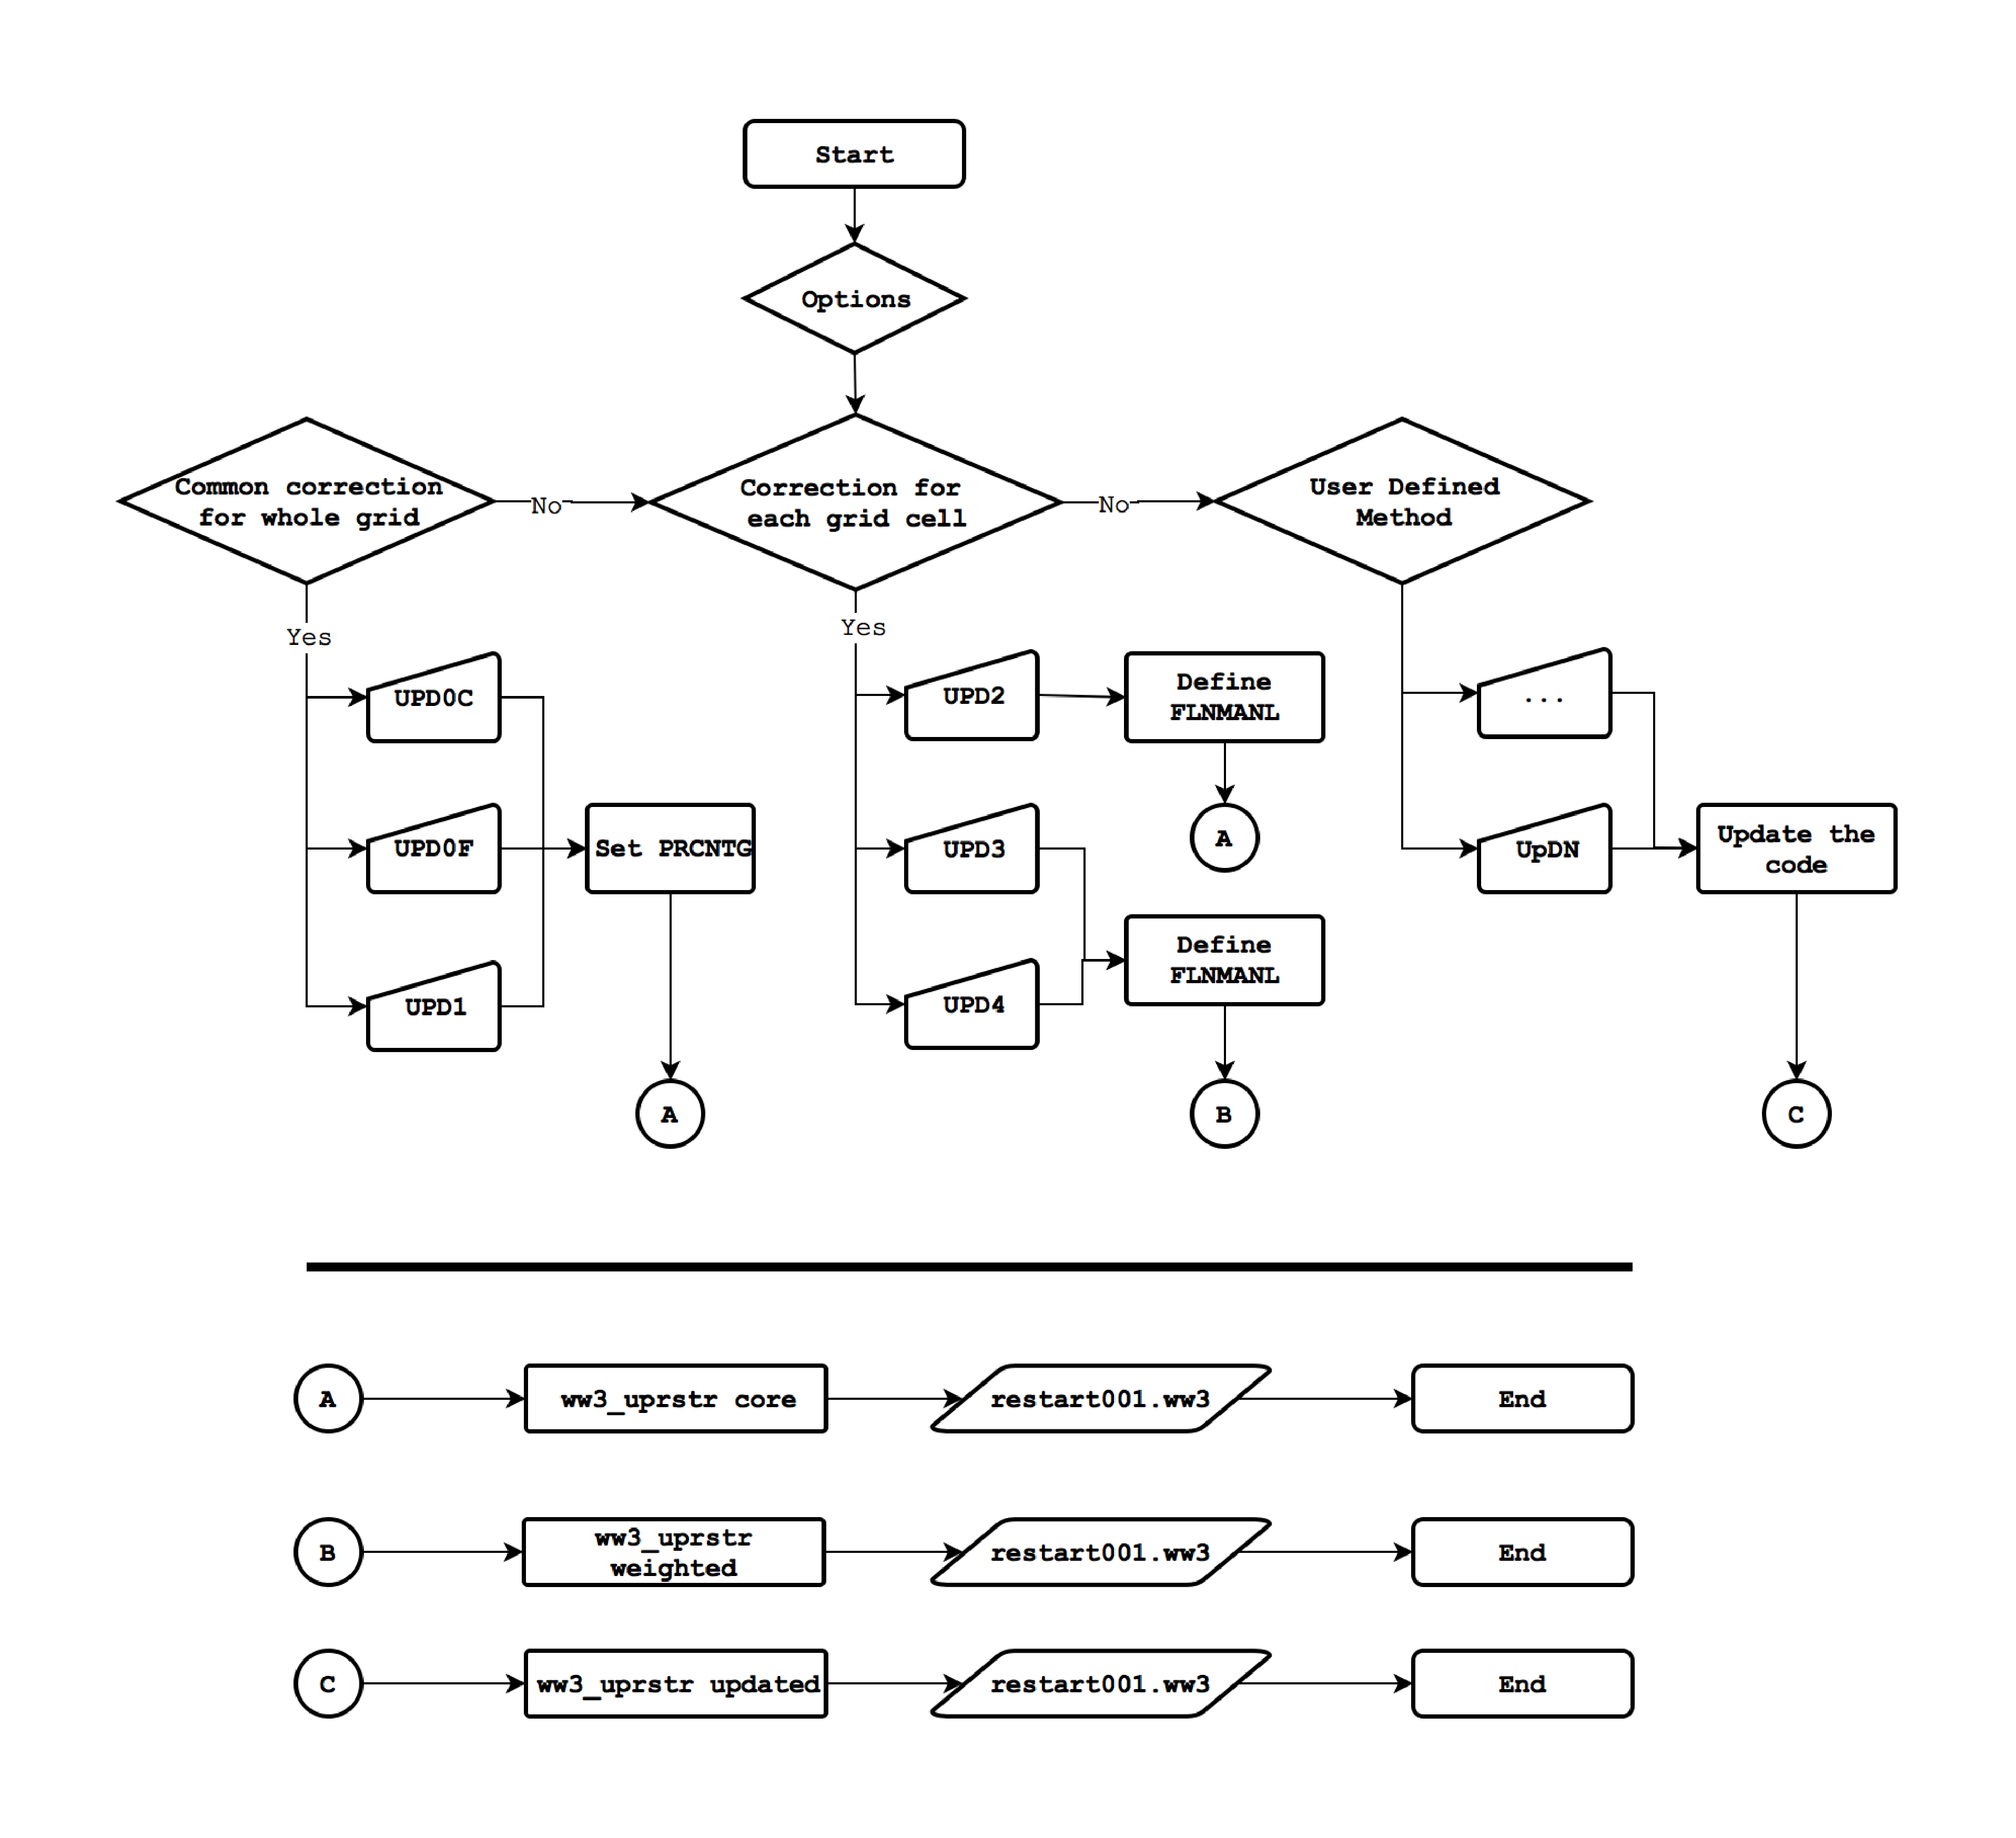
\includegraphics[width=0.9\textwidth]{./run/uprstr.eps}
\caption{Flowchart of the implemented methods for updating the wave spectra at the WW3 
restart file. Additional methods can be implemented by adding UPD options to the namelist.}
\label{fig:uprstrflowchart} \botline
\end{center}
\end{figure}

The following UPD options are available:
\begin{enumerate} 
   \item UPD0C:: Option 0C  All the spectra are updated with a constant 
      fac=(SWH\_Bckg-SWH\_Anl)/SWH\_Anl.
   \item UPD0F:: Option 0F  All the spectra are updated with a constant 
      fac=SWH\_Anl/SWH\_Bckg. 
   \item UPD1 :: Option 1   The fac(x,y,frq,theta), is weighted according to
      the \% of energy at each spectral bin; fac the same as UPDOF.
   \item UPD2 :: Option 2   The fac(x,y,frq,theta), is calculated at 
         each grid point according to SWH\_Bckg and SWH\_Anl
   \item UPD3 :: Option 3   The update factor is a surface with the shape of 
      the background spectrum. 
   \item UPD4 :: [NOT INCLUDED in the current version, just keeping the spot]
      Option 4  The generalization of the UPD3. The update factor is the sum of surfaces 
      which are applied on the background spectrum 
\end{enumerate}

Any additional method for the redistribution of the energy to the WS could be added 
by adding a new entry at the namelist of the \textbf{ww3\_uprstr.inp}.

\subparagraph{Example \newline}
In this section, an example of the simplest WDA application is discussed.
The figure ~\ref{fig:waveDAflowchart} shows how the \textbf{ww3\_uprstr} 
is used in the framework of a simple wave analysis system. \newline

A WW3 run (from the previous cycle or from the warm up of the model) provides the
background field of SWH and the corresponding restart file at the appropriate time. 
The format of the background SWH field has to be compatible with the WDA module inputs.

The WDA module uses the background field and the available observations
for the time of analysis, produces the analysis (\textbf{XXXX.grbtxt}) and exports 
the field of SWH in grbtxt format.

The analysis file, the mod\_def.ww3, the restart.ww3 file and the ww3\_uprstr.inp 
are the input files for the \textbf{ww3\_uprstr}. If all the options and input 
files are correctly prepared, it takes approxmately one minute to update a grid 
of 260000 grid nodes and generate the output on a single processor. 
The updated restart file has to be renamed, at the expected file name, in the case of this
example restart.ww3. \newline  

   \fbox{
      \parbox{\textwidth}{
      \textbf{Note: }
      All \ncep's WDA systems use GRIB2 format, thereore there is always an intermediate
      step to transfer the grib files to the appropriate format. The used software is WGRIB2 
      and more information can be retrieve from the 
      \href{http://www.cpc.ncep.noaa.gov/products/wesley/wgrib2} {official website}.       
      }
   }

\begin{figure} \begin{center}
\includegraphics[width=0.9\textwidth]{./run/waveDA.eps}
\caption{Flowchart of simplified wave data assimilation system, 
showing the role of the {ww3\_uprstr}, the required input files,
and the resulted output of the updated restart file.}
\label{fig:waveDAflowchart} \botline
\end{center}
\end{figure}

%\paragraph{How to Update the ww3\_uprstr \newline}
%Add data readers, mainly for machine independent binary data and wgrib2.

\pb


% tab:fields

\begin{table} \begin{center}
\begin{tabular}{|c|c|c|c|c|c|} \hline
group & field & description                  &  file        & GRIB1 & GRIB2   \\
      &                              &  extension   & data  & data    \\ \hline \hline
 1 & 1 & depth                           & {\file .dpt} &  --  &    --    \\
 1 & 2 & mean current components         & {\file .cur} &  --  &    --    \\
 1 & 3 & wind speed                      & {\file .wnd} &  32  &  0,2,1   \\
   &&  wind direction                 &              &  31  &  0,2,0   \\
   &&  wind $u$                       &              &  33  &  0,2,2   \\
   &&  wind $v$                       &              &  34  &  0,2,3   \\
 1 & 4 & air-sea temp. dif.              & {\file .dt}  &  --  &    --    \\
 1 & 5 & water level                     & {\file .wlv} &  --  &  10,3,1  \\
 1 & 6 & ice coverage                    & {\file .ice} &  91  &  10,2,0  \\
 2 & 1 & wave height $H_s$               & {\file .hs}  & 100  &  10,0,3  \\
 2 & 2 & mean wave length                & {\file .l}   &  --  &    --    \\
 2 & 3 & mean wave period $T_{m0,2}$     & {\file .t02} &  --  &    --    \\
 2 & 4 & mean wave period $T_{m0,1}$     & {\file .t}   & 103  &  10,0,15 \\
 2 & 5 & mean wave period $T_{m0,-1}$    & {\file .tm1} &  --  &    --    \\
 2 & 6 & peak frequency $f_p$            & {\file .fp}  & 108  &  10,0,11 \\
 2 & 7 & mean wave direction $\theta_m$  & {\file .dir} & 101  &    --    \\
 2 & 8 & directional spread $\sigma$     & {\file .spr} &  --  &    --    \\
 2 & 9 & peak direction $\theta_p$       & {\file .dp}  & 107  &  10,0,10 \\
 4 & 1 & $H_s$ of partition              & {\file .phs} & 102,105 & 10,0,5/8 \\
 4 & 2 & $T_p$ of partition              & {\file .ptp} & 110,106 & 10,0,6/9\\
 4 & 3 & $L_p$ of partition              & {\file .plp} &  --  &    --    \\
 4 & 4 & $\theta_m$ of partition         & {\file .pdir} & 109,104 & 10,0,4/7 \\
 4 & 5 & $\sigma$ of partition           & {\file .psi} &  --  &    --    \\
 4 & 6 & wind sea fraction of part.      & {\file .pws} &  --  &    --    \\
 4 & 7 & total wind sea fraction         & {\file .wsf} &  --  &    --    \\
 4 & 8 & number of partitions            & {\file .pnr} &  --  &    --    \\
 5 & 1 & friction velocity comp.         & {\file .ust} &  --  &    --    \\
 5 & 2 & Charnock parameter for air side & {\file .cha} &  --  &    --    \\
 5 & 3 & Energy flux $\int C_g E(f) df$  & {\file .CgE} &  --  &    --    \\
 5 & 4 & Wind to wave energy flux        & {\file .faw} &  --  &    --    \\
 5 & 5 & Wave-supported stress           & {\file .taw} &  --  &    --    \\
 5 & 6 & Upward wave-supported stress    & {\file .twa} &  --  &    --    \\
 5 & 7 & Whitecap coeverage              & {\file .wcc} &  --  &    --    \\
 5 & 8 & Average whitecap foam thickness & {\file .wcf} &  --  &    --    \\
 5 & 9 & Significant breaking wave height& {\file .wch} &  --  &    --    \\
 5 & 10 & Whitecap moment                 & {\file .wcm} &  --  &    --    \\ \hline
\end{tabular} \end{center}
\caption{~Field output post processors ancillary data.} \label{tab:fields}
\vspace{0.5in}
\end{table}

\begin{table} \begin{center}
\begin{tabular}{|c|c|c|c|c|c|} \hline
group & field & description                  &  file        & GRIB1 & GRIB2   \\
      &                              &  extension   & data  & data    \\ \hline \hline
 6 & 1 & radiation stress                & {\file .Sxy} &  --  &    --    \\
 6 & 2 & Breaking wave momentum flux     & {\file .two} &  --  &    --    \\
 6 & 3 & Bernoulli head                  & {\file .J} &  --  &    --    \\
 6 & 4 & Breaking wave energy flux       & {\file .foc} &  --  &    --    \\
 6 & 5 & Stokes transport                & {\file .tus} &  --  &    --    \\
 6 & 6 & Surface Stokes drift            & {\file .uss} &  --  &    --    \\
 6 & 7 & Second order pressure at $k=0$  & {\file .p2s} &  --  &    --    \\
 7 & 1 & near-bottom amplitude           & {\file .cfd} &  --  &    --    \\
 7 & 2 & near-bottom velocity            & {\file .ubr} &  --  &    --    \\
 7 & 3 & bedform parameters              & {\file .bed} &  --  &    --    \\
 7 & 4 & Energy flux to bot. boundary layer & {\file .fbb} &  --  &    --    \\
 7 & 5 & Momentum flux to bot. boundary layer & {\file .tbb} &  --  &    --    \\
 8 & 1& mean square slopes              & {\file .mss} &  --  &    --    \\
 8 & 2 & Phillips constant               & {\file .msc} &  --  &    --    \\
 9 & 1 & average time step               & {\file .dtd} &  --  &    --    \\
 9 & 2 & cut-off frequency $f_c$         & {\file .fc}  &  --  &    --    \\
 9 & 3 & cut-off frequency $f_c$         & {\file .fc}  &  --  &    --    \\
 9 & 4 & maximum CFL for X-Y advection   & {\file .cfx} &  --  &    --    \\
 9 & 5 & maximum CFL for $\theta$ advection & {\file .cfd} &  --  &    --    \\
 9 & 6 & maximum CFL for $k$ advection   & {\file .cfk} &  --  &    --    \\
 10 & 1 & user defined \#1                & {\file .us1} &  --  &    --    \\
 10 & 2 & user defined \#2                & {\file .us2} &  --  &    --    \\ \hline
%13 & wind sea period $T_w$           & {\file .fpl} & 110  &    --    \\
%14 & wind sea direction $\theta_w$   & {\file .dpl} & 109  &    --    \\

\end{tabular} \end{center}
\caption*{Table~\ref{tab:fields}, continued.} 
\vspace{0.5in}
\end{table}

\clearpage

%\bpage

\section{~Install, Compile and Run the wave model} \label{chapt:impl}
\newcounters

\vssub
\subsection{~Introduction}
\vssub

\ws\ is written in ANSI standard \fortran-90, with no machine-dependent
elements, so that \ws\ can be installed without modifications on most
platforms. \ws\ utilizes its own preprocessor to select model options at the
compile level, and to switch test output on or off. This approach proved to be
efficient during the development of \ws, but complicates its installation. 
To minimize complications, a set of \unix/Linux scripts is provided to
automate the installation in general and the use of the preprocessor in
particular. 
Note this option is not supported for other operation systems like MS
products. If the code is to be compiled on one of the latter platforms, it is
suggested to extract a working code in a \unix/Linux environment using the
utility {\code w3\_source} (see below), and then to port this clean code to
the platform of choice.

\begin{center}
\rule[1mm]{55mm}{1.0mm} WARNING \rule[1mm]{55mm}{1.0mm} \\ 
\vspace{\baselineskip}
\parbox{120mm}{If version \WWver\ is implemented as an upgrade to previous
versions of \ws, please note that this version may not be compatible with
previous model versions. It is therefore prudent {\it NOT} to install the new
version of \ws\ on top of the old version.} \\ \vspace{\baselineskip}
\rule[1mm]{55mm}{1.0mm} WARNING \rule[1mm]{55mm}{1.0mm}
\end{center}

\vssub
\subsection{~Installing files}\label{sec:install}
\vssub

\noindent
In its packaged public version (tar file distribution), \ws\ is
contained in several files:

\begin{list}{???}{\parsep 0mm \itemsep 0mm 
                  \leftmargin 20mm \rightmargin 5mm
                  \labelwidth 10mm \labelsep 5mm}
\item[{\file install\_wwatch3\_tar} \hfill]
The \ws\ install program. 

\item[{\file wwatch3.[VERTAG].model.tar} \hfill] Archive file containing 
 source codes (ftn directory), programs and scripts controlling the
compiling and linking of and code management of \ws (aux and bin
directories), and sample input files (inp directory).

\item[{\file wwatch3.[VERTAG].regtests.tar} \hfill]
Archive file containing several regression test cases.

\item[{\file wwatch3.[VERTAG].cases.tar} \hfill]
Archive file containing several large tests involving real case scenarios. 

\end{list}

\noindent
The label [VERTAG] is typically a version number for the model package, which
may be followed or preceded by alpha-numeric tags describing other
characteristics of the distribution package (e.g., v4.18.beta for the beta
version 4.18 etc).

As the first step of installing \ws, these files have to be copied to a work
directory on the machine on which \ws\ will be installed. Because this
directory will be the `home' directory of \ws, it is suggested that a new
directory is created (see also warning in previous section). Furthermore
{\file install\_wwatch3\_tar} has to be made executable by typing
\command{chmod 700 install\_wwatch3\_tar} after which the installation of the
files is started by typing \command{install\_wwatch3\_tar} at your Linux/Unix
prompt.


\begin{center}
\rule[1mm]{55mm}{1.0mm} WARNING \rule[1mm]{55mm}{1.0mm} \\ 
\vspace{\baselineskip}

\parbox{120mm}{The install program will ask for a compiler to compile some
auxiliary \fortran\ codes. Unlike the actual \ws\ source code, these programs
are still written in \fortran-77. It is therefore sufficient to point toward
the generic \fortran-77 compiler on the system. The {\file install\_ww3\_tar}
script allows the user to set pre-defined choices that will point the
\fortran-77 to a generic executable {\file f77}. This may not be available on
your system, so make sure that an appropriate choice is made during the
installation process.}
\\ \vspace{\baselineskip} \rule[1mm]{55mm}{1.0mm}
WARNING \rule[1mm]{55mm}{1.0mm}
\end{center}

When {\file install\_wwatch3\_tar} is executed for the first time, it will ask
the user to identify the directory in which \ws\ will be installed. This has
to confirm that the installation directory is the current directory. Next, the
script jumps to the most crucial option, which determines if a local or generic install 
is to be performed.

The type of install deals with where to save the the traditional {\file wwatch3.env} 
file, containing the general user-dependent directory and basic FORTRAN and C compiler 
choices. The local install will save this at the same location as the package
is being installed, which is the main \ws\ directory. This results in a standalone version
that allows multiple installations (or other branches or the trunk) to co-exist
without interference. The general install means wwatch.env will be save in the user's
home directory in the form {\file \$HOME/.wwatch3.env}, and that this will be the
main or central installation in that work area. The existence of a general install
does not preclude the existence of multiple local installs, but the user has to be 
mindful of which code is being invoked when using the general install (things can
get very confusing if not kept explicitly on track).

After a choice is made for local or generic install, the script will search for
existing config files. If none is found, it will print a message that it cannot find 
the setup file, and ask some questions. The same questions are asked if a setup file is found,
except that the intention there is to confirm the existing options have not changed. In any case,
having a pre-existing setup or not, the script will give the user an opportunity to revise
defaults/existing and change if needed. The script will echo the existing options, and the 
default/existing answers or options are shown in square brackets. 

Other than the generic or local wwatch.env files, a third alternate
setup file may be specified prior to running {\file install\_wwatch3\_tar} by
setting {\code WWATCH3\_ENV} in the user environment.  The setup can be
modified by rerunning the install program, or by manually editing the setup
file. The `home' directory of \ws\ can only be changed by editing or removing
thelocal or generic {\file wwatch3.env} or by changing {\code WWATCH3\_ENV} in the user
environment.

\begin{center}
\rule[1mm]{55mm}{1.0mm} WARNING \rule[1mm]{55mm}{1.0mm} \\ 
\vspace{\baselineskip}

\parbox{120mm}{In case you decide to use the generic installation, you have to make sure
that the model installation directory is either {\file \${HOME}/wwatch3} or if it has
a different name, it is linked to {\file \${HOME}/wwatch3}. If this is not the case
the generic install may fail or compromise other pre-existing installations.}
\\ \vspace{\baselineskip} \rule[1mm]{55mm}{1.0mm}
WARNING \rule[1mm]{55mm}{1.0mm}
\end{center}

After the setup file is processed, the install program asks if the user wants
to continue with the installation. If the user chooses to continue, the
program will look for the archive files. If no files are found, the
archive files do not reside in the home directory, or the home directory is
erroneously defined, the installation will exit. 
Check the location of the archive files, and the `home' directory of \ws\
(see previous paragraphs).

After files to be unpacked have been identified, the program will ask if old
files should be overwritten automatically. If the user chooses `n', the
program will ask permission to overwrite each file that already exists. Files
that contain user specific information, such as compile and link options, will
never be replaced by the install program.

As the first step of the actual installation, the install program checks if
the following directories exist in the `home' directory of \ws.
 
\begin{dlist}
\dit{arc }{Archive directory.}
\dit{aux }{Raw auxiliary programs (source codes etc.).}
\dit{bin }{Executables and shell scripts for compiling and linking.}
\dit{exe }{\ws\ executables.}
\dit{ftn }{Source code and makefile.}
\dit{inp }{Input files.}
\dit{mod }{Module files.}
\dit{obj }{Object files.}
\dit{test}{Scripts with test cases.}
\dit{work}{Auxiliary work directory.}
\end{dlist}

\noindent
All these directories are generated by the install program {\file
install\_wwatch3}, except for the archive directory, which is generated by
{\file arc\_wwatch3} (see below).

Unlike previous version, where the user could choose which parts of the
package were to be installed, the current {\file install\_ww3\_tar} script
installs the etinre updated package without prompting. 

Installation of the auxiliary programs will first process source codes of
auxiliary programs, using the compiler as defined by the user in the setup
file. Note that these codes are still in fixed format \fortran-77.

\begin{flist}
\fit{w3adc.f }{\ws\ {\fortran} preprocessor.}
\fit{w3prnt.f}{Print files (source codes) including page and line numbers.}
\fit{w3list.f}{Generate a generic source code listing.}

\fit{w3split.f}{Generate spectral bulletin identifying individual wave fields
  within a spectrum from the spectral output of the point output
  post-processor (see \para\ref{sec:ww3outp}). This is a legacy code
  superseded by generating bulletins directly from {\file ww3\_outp}. It is
  retained here for historical reasons only.}

\end{flist}

\noindent
The above source codes are stored in the directory {\dir aux} and the
executables are stored in the directory {\dir bin}. A more detailed
description of these programs (including instructions on running the
executables) can be found in the documentation included in the above source
code files. After the compilation of these programs, several \unix\ shell
scripts and auxiliary files are installed in the {\dir bin} directory.

\begin{flist}
\fit{ad3              }{Script to run the preprocessor {\file w3adc}
                        and the compile script {\file comp} for a given
                        source code file.}
\fit{ad3\_test        }{Test version of {\file ad3}, showing modifications
                        to original source file. This script does not
                        compile code.}
\fit{all\_switches    }{Generates a list of all {\code w3adc} switches 
                        present in the source code files.}
\fit{arc\_wwatch3     }{Program to archive versions of \ws\ in the 
                        directory {\dir arc}.}
\fit{comp.gen         }{Generic compiler script. The actual compiler
                        script {\file comp} will be copied from this
                        script if it does not exists.}
\fit{comp.{\it xxx}   }{The compiler script {\file comp} for a specific
                        hardware-compiler combination.}
\fit{find\_switch     }{Script to find \ws\ source code files containing 
                       compiler switches (or arbitrary strings).}
\fit{install\_ww3\_svn }{Script to install \ws\ from the svn repository.}
\fit{install\_ww3\_tar }{Script to install \ws\ from tar files.}
\fit{link.gen         }{Generic linker script. Actual script is {\file
                        link}.}
\fit{link.{\it xxx}   }{The link script {\file comp} for a specific
                        hardware-compiler combination.}
\fit{list             }{Script to print source code listing using 
                        {\file w3prnt}.}
\fit{ln3              }{Script to make symbolic link of source code file
                        to work directory.}
\fit{make\_MPI        }{Script to separately compile MPI and non-MPI programs.}
\fit{make\_OMP        }{Script to separately compile OpenMP and single threaded
                        programs.}
\fit{make\_HYB        }{Script to separately compile hybrid MPI-OpenMP and
                        single threaded programs.}
\fit{make\_makefile.sh}{Script to generate the of the makefile based
                        on selections in the file {\file switch})}. 
\fit{switch.gen       }{Generic file with preprocessor switches
                        (\para\ref{sec:switches}).}
\fit{switch.{\it xxx}       }{Examples of preprocessor switches
                        provided by users or developers.}
\fit{w3\_clean        }{Script to clean up work and scratch directories
                        by removing files generated during compilation or
                        test runs.}
\fit{w3\_make         }{Script to compile and link components of \ws\
                        using a makefile.}
\fit{w3\_new          }{Script to touch correct source code files
                        to account for changes in compiler switches in
                        combination with the makefile.} 
\fit{w3\_setup        }{Script for creating/editing the \ws\ environment setup
                        file. The default setup file is
                        {\file \$\{HOME\}/.wwatch3.env}.  An alternate setup
                        file can be specified with the {\code WWATCH3\_ENV}
                        environment variable.}
\fit{w3\_source       }{Script to generate a true \fortran\ source
                        code for any of he \ws\ program elements.}
\fit{ww3\_gspl.sh     }{Script to automate use of {\file ww3\_gspl} program 
                        (see \para\ref{sub:ww3gspl}).}
\end{flist}

\noindent
The use of these scripts is explained in \para\ref{sec:comp}.  Note that the
above scripts acquire setup information from the \ws\ environment setup file
defined by {\code WWATCH3\_ENV}, or, if that is not defined, from the generic 
setup file {\file .wwatch3.env} in the home directory of the user, or the local 
setup file {\file wwatch3.env} in the directory where the wave model package is 
being installed.

\noindent
After installation in the {\dir bin} directory, several GrADS scripts are
installed in the {\dir aux} directory.

\begin{flist}
\fit{cbarn.gs         }{Semi-standard GrADS script for displaying
                        color bars.}
\fit{colorset.gs      }{Script to define colors used in shading.}
\fit{profile.gs}      {Script to display profiling data generated by {\file
                       ww3\_multi}.} 
\fit{source.gs}       {Script for composite plot of spectra and source
                       terms (2-D polar or Cartesian plots in color or in
                       black and white).}
\fit{1source.gs}      {Script to plot single source term.}
\fit{spec.gs}         {Script to plot spectra.}
\fit{spec\_ids.gen}   {Data file used by spectral / source scripts.}
\end{flist}

\noindent
This directory also has various additional tools in and documentations, see
the actual directory for its contents. These include contributed {\it Matlab} scripts,
{\file IDL} scripts and tools, and a manual on using {\file SMG type} grids.

As the final step of {\file aux} processing, some links between directories are established.

Finally, the install program lists manual modifications required by or
suggested to the user. These messages are printed only if the compile and link
system are installed. An example of an installation session using the script
{\file install\_ww3\_tar} is provided below for a case where local install was
chosen.

\pb

%\begin{myfig}{tbp}
\begin{minipage}[c]{4.5in}
{\scriptsize \begin{verbatim}
GUIDE >> tar zxvf wwatch3.beta.v4.18.tar.gz 
install_ww3_tar
guide.beta.v4.18.pdf
manual.beta.v4.18.pdf
wwatch3.beta.v4.18.model.tar
wwatch3.beta.v4.18.regtests.tar

GUIDE >> ls -l
total 354836
-rw-------. 1 wd20ha wd2    197909 Jan 14 10:11 guide.beta.v4.18.pdf
-rwx------. 1 wd20ha wd2     38670 Jan 14 10:12 install_ww3_tar
-rw-------. 1 wd20ha wd2   3545855 Jan 14 10:12 manual.beta.v4.18.pdf
-rw-------. 1 wd20ha wd2 135690240 Jan 14 10:12 wwatch3.beta.v4.18.model.tar
-rw-------. 1 wd20ha wd2 123136000 Jan 14 10:12 wwatch3.beta.v4.18.regtests.tar
-rw-------. 1 wd20ha wd2 100731957 Mar 13 15:05 wwatch3.beta.v4.18.tar.gz

GUIDE >> ./install_ww3_tar 


                  ===================================
              ------ Installing WAVEWATCH III  v.4 ------
                  =================================== 

                  Script for installing package from tar files. 
                  Requires files in same directory as script.

 Continue? [y|n] y


                  ===================================
              ------ Installing WAVEWATCH III  v.4 ------
                  ===================================
                                     from tar source 

 This installation requires a configuration file (wwatch3.env).
 The current version allows two types of env files: 
 - A local [L] wwatch3.env (Allowing multiple independent installations).
 - A generic [G] dot-file .wwatch3.env (Old-fashioned option).
 [L] Installs new, uses existing or updates env file in current directory.
 [G] Installs new, uses existing or updates env file in home directory, 
     (home is presumably /export/emc-lw-jhalves/wd20ha}). 

 Type your choice now: G

 Installing in 
   /export/emc-lw-jhalves/wd20ha/WW3_GUIDE

   OK ? [y/n] y

\end{verbatim}}
\end{minipage}

\begin{minipage}[c]{4.5in}
{\scriptsize \begin{verbatim}

 Setting up environment variables. 


   Previous setup file not found. Variables will be set to defaults. 

     (User must check to see if these setting are appropriate.)      


 Creating wwatch3.env locally (also in home if G option chosen). 
      Printer (listings)       : printer 
      FORTRAN comp. (aux only) : f77 
      C Compiler (aux only)    : cc 
      Scratch directory        : /export/emc-lw-jhalves/wd20ha/WW3_GUIDE/tmp 
      Save source code         : yes 
      Save listings            : yes 

 Update settings ? [y/n] y

 Modifying set-up 

 Type n new settings, or press ENTER to keep [current ones]: 

      Printer for listings [printer] : 
      Compiler for aux. [f77] : gfortran
      Compiler for aux. [cc] : gcc
      Scratch space [/export/emc-lw-jhalves/wd20ha/WW3_GUIDE/tmp] : 
      Save source code files (*.f)  [yes] : 
      Save listing files  [yes] : 
 
   Modified settings:
      Printer (listings)       : printer 
      FORTRAN comp. (aux only) : gfortran 
      C Compiler (aux only)    : gcc 
      Scratch directory        : /export/emc-lw-jhalves/wd20ha/WW3_GUIDE/tmp 
      Save sources             : yes 
      Save listings            : yes 

   New settings OK ? [y/n]  y

 Continue with actual implementation ? [y/n] y


[==========================SCREEN OUTPUT OMMITTED=============================]


\end{verbatim}}
\end{minipage}

\begin{minipage}[c]{4.5in}
{\scriptsize \begin{verbatim}
=============================== 
 --- Final remarks ---
 ============================================================== 

 To run the WAVEWATCH III executables and the scripts to generate 
 and update these executables from arbitrary directories, add the
 following directories to the path of your interactive shell : 

      /export/emc-lw-jhalves/wd20ha/WW3_GUIDE/bin
      /export/emc-lw-jhalves/wd20ha/WW3_GUIDE/exe

 Note that 'comp' and 'link' and 'switch' are user/machine specific.

   Several comp and link files for known compilers are found in:
   /export/emc-lw-jhalves/wd20ha/WW3_GUIDE/bin

   If you cannot find one that suits your machine/preferences, 
   create custom scripts based on the existing ones and add to bin.


                    ===============================
                  ---       End of program        --- 
                    =============================== 
 

GUIDE >> ls -l
total 3708
drwx------.  2 wd20ha wd2    4096 Mar 13 15:45 arc
drwx------.  6 wd20ha wd2    4096 Mar 13 15:45 aux
drwx------.  2 wd20ha wd2    4096 Mar 13 15:45 bin
drwx------.  2 wd20ha wd2    4096 Mar 13 15:45 exe
drwx------.  3 wd20ha wd2    4096 Mar 13 15:45 ftn
-rw-------.  1 wd20ha wd2  197909 Jan 14 10:11 guide.beta.v4.18.pdf
drwx------.  2 wd20ha wd2    4096 Mar 13 15:45 inp
lrwxrwxrwx.  1 wd20ha wd2      21 Mar 13 15:45 install_ww3_tar -> ./bin/install_ww3_tar
-rw-------.  1 wd20ha wd2 3545855 Jan 14 10:12 manual.beta.v4.18.pdf
drwx------.  2 wd20ha wd2    4096 Mar 13 15:45 mod
drwx------.  2 wd20ha wd2    4096 Mar 13 15:45 obj
drwx------. 40 wd20ha wd2    4096 Mar 13 15:45 regtests
drwx------.  2 wd20ha wd2    4096 Mar 13 15:45 tmp
drwx------.  2 wd20ha wd2    4096 Mar 13 15:45 work
-rw-------.  1 wd20ha wd2     324 Mar 13 15:44 wwatch3.env

\end{verbatim}}
\end{minipage}


\pb
\vssub
\subsection{~Optional environment settings}
\vssub

Compilation of the \ws\ NetCDF enabled programs requires the environment variable
{\code WWATCH3\_NETCDF} be set to either {\code NC3} (compile with NetCDF
version 3.x) or {\code NC4} (compile with NetCDF version 4.x).  If the script
variable is set to {\code WWATCH3\_NETCDF = NC3}, then the following
environment variables are required
\begin{clist}
\cit {NETCDF\_LIBDIR} {Path to where the NetCDF-3 libraries are installed.}
\cit {NETCDF\_INCDIR} {Path to where the NetCDF-3 include files are installed.}
\end{clist}
If {\code WWATCH3\_NETCDF = NC4}, then the following environment variable
is required.
\begin{clist}
\cit {NETCDF\_CONFIG} {Path to the NetCDF-4 nc-config utility program.}
\end{clist}
The {\file nf-config} utility program (part of the NetCDF-4 install or 
{\file nc-config} for old versions) is used to determine the appropriate
compile and link flags for the {\code WWATCH3\_NETCDF = NC4} compile.
The NetCDF-4 compile requires NetCDF version 4.1.1 or higher.  Use the command
\command{\code nf-config --version} to check the version of the installed 
Fortran-NetCDF library.  Compiling with the {\code NC4} switch requires
{\code WWATCH3\_NETCDF = NC4} and the NetCDF-4 installation compiled with the
NetCDF-4 API enabled.  Use \command{\code nf-config --has-nc4} to check if the
installed NetCDF has the NetCDF-4 API enabled.

\vspace{\baselineskip} 
\noindent
Compilation of the WAVEWATCH III with PDLIB for Domain Decompstion option
for (Explicit/Implicit) triangular unstructed grids requires the environment
variable {\code METIS\_PATH} be set to the path where {\code Metis} and
{\code ParMetis} are compiled using the same compiler used for WW3.

\vspace{\baselineskip}
\noindent
Two additional remarks need to be made regarding parallel versions of the
model (OpenMP and \mpi\ versions). First, complications may occur when
preparing executables for running in an \mpi\ environment. Such complications
are discussed in Appendix~\ref{app:mpi}. Secondly, the \omp\ code should be
compiled using directives only, i.e., do not use compiler options that
automatically thread the code.



\vssub
\subsection{~Compiling and linking} \label{sec:comp}
\vssub

\vspace{\baselineskip} \noindent 
For the first compilation, the \ws\ environment must be set up using the script
{\file w3\_setup} with the model directory path in argument. Some options are
available to define the compiler options and the switch file located in the
{\dir bin} directory. For instance, \command{w3\_setup /home/user/WW3/model
-c <comp> -s <switch>} the {\code <comp>} keyword can be {\code mpt}, 
{\code intel}, {\code gfortran}, {\code pgi} for optimized compilation options
or could be {\code mpt\_debug}, {\code intel\_debug}, {\code gfortran\_debug},
{\code pgi\_debug} for debugging compilation options. If system-dependant
options are needed, it can be done by modifying the script {\file cmplr.env}. 
Some old comp/link templates from different clusters are still available but 
not recommended. The {\code <switch>} keyword can be the suffix of a provided
switch file or your own one. Running this script will create these three 
scripts/files :

\begin{flist}
\fit{comp}  {Compiler script. This script is based on {\file comp.tmpl} with
	    the provided definition of the compiler and its options.}
\fit{link}  {Linker script. This script is based on {\file link.tmpl} with
	    the provided definition of the linker and its options.}
\fit{switch}{File containing a list of switches as recognized by the
             preprocessor {\file w3adc}. Copied from {\code switch\_<switch>}}.
\end{flist}

\vspace{\baselineskip}

The environment file {\file wwatch3.env} will be created or updated if it 
already exists. The auxiliary FORTRAN programs for code prepocessor will be
compiled using by default the GNU FORTRAN compiler which can be different to
the provided compiler for the \ws\ programs.


\vspace{\baselineskip} \noindent 
The easiest way to compile \ws\ is using the script {\file w3\_automake} to 
automatically detect which programs to compile and to compile it. It will
force pre- and post-processing programs to be compiled as sequential 
implementation and others depending on the switches from openMP, MPI or hybrid
configurations. If the netCDF library is correctly set up, the netCDF dedicated
programs will be also compiled. The same test is done for SCRIPNC, PDLIB, OASIS,
ESMF, TRKNC and TIDE keywords to manage the program compilation in the best way.
For instance, \command{w3\_automake} or for a few programs \command{w3\_automake
ww3\_grid ww3\_shel ww3\_ounf} the compiled programs will all be stored in the 
{\dir exe} directory with a copy of the switch, comp and link files used.

\vspace{\baselineskip} \noindent
In case of troubles during the compilation of a program, the log files will be
stored in a temporary directory which will differs between sequential mode
({\dir tmp\_SEQ}) and distributed mode like MPI ({\dir tmp\_MPI}), OMP 
({\dir tmp\_OMP}) or hybrid ({\dir tmp\_HYB}). There are usually three log files
per program:

\begin{flist}
\fit{\code ww3\_<prog>.l} {full program with only the matching lines
	of codes based on the switches and at the end the compilation command line.}
	\fit{\code ww3\_<prog>.out} {warning messages}
	\fit{\code ww3\_<prog>.err} {error messages}
\end{flist}

To remove all user-created files from the \ws\ framework, the script 
{\file w3\_clean} can be used by only cleaning up the {\dir model} directory
\command{w3\_clean -m} or the full ww3 repository \command{w3\_clean -c}


\vssub
\subsection{~Detailled compilation}
\vssub

Compilation of \ws\ is performed using the script {\file w3\_make} in the
{\dir bin} directory\footnote{~Note that before running {\file w3\_make}
  several user interventions are needed as described in the remainder of this
  section.}.  If this script is used without parameters, all basic programs of
\ws\ are compiled. Optionally, names of programs to be compiled can be given
as part of the compile command. For instance \command{w3\_make ww3\_grid
  ww3\_strt} will compile the grid preprocessor and the initial conditions
program only. {\file w3\_make} uses several of the scripts described in the
previous section. A graphical representation is given in Fig.~\ref{fig:make}.
If necessary, the script {\file w3\_make} uses the scripts {\file
  make\_makefile.sh} to generate a makefile. {\file make\_makefile.sh}
generates a list of modules to be linked, based on the program switches in the
file {\file switch} (see~\para\ref{sec:switches}), and checks all needed
sources for module dependencies. If switches have been changed since the last
call to {\file w3\_make}, {\file w3\_new} is used to `touch' relevant source
code or to delete relevant object files. After the makefile has been
completed, the standard \unix\ make utility is used to compile and link the
programs. Instead of directly using the \fortran\ compiler, the makefile
invokes the preprocessor and compile scripts {\file ad3} and {\file comp}, and
the link script {\file link}. The script {\file ad3} uses the extension of the
file name to determine the necessary action. Files with extension {\file .ftn}
are processed by {\code w3adc}, files with extension {\file .f} or {\file
  .f90} are send to the script {\code comp} directly.  Although a user could
try out several of these scripts interactively, he or she generally needs to
run {\file w3\_make} only.

\setlength{\unitlength}{0.1mm}

\begin{figure}
\begin{picture}(1370,550)(0,-490)

\scripta{  85}{   0}{w3\_make}
\scriptb{ 335}{-100}{make\_makefile.sh}
\scriptc{ 335}{-200}{make}
\put(185,-170){\line(0,1){170}}
\multiput(185,-170)(0,100){2}{\line(1,0){150}}

\scripta{ 785}{-100}{w3\_new}
\scripta{ 785}{-200}{ad3}
\scripta{ 785}{-400}{link}
\put(785, -70){\line(-1,0){100}}
\put(785,-170){\line(-1,0){100}}
\put(785,-370){\line(-1,0){ 50}}
\put(735,-370){\line(0,1){200}}

\scripta{1085}{-200}{w3adc}
\scripta{1085}{-300}{comp}
\put(1085,-170){\line(-1,0){100}}
\put(1085,-270){\line(-1,0){ 50}}
\put(1035,-270){\line(0,1){100}}

\sscript{ 300}{   0}{1}
\sscript{ 700}{-100}{1,2,3}
\sscript{1000}{-100}{1}
\sscript{1000}{-200}{1}
\sscript{1300}{-200}{4}

\sscript{50}{-350}{1}
\put(80,-330){\makebox(-1000,60)[l]{\small Suitable for interactive use.}}
\sscript{50}{-400}{2}
\put(80,-380){\makebox(-1000,60)[l]{\small If {\file makefile} does not exist.}}
\sscript{50}{-450}{3}
\put(80,-430){\makebox(-1000,60)[l]{\small If switch file has been updated.}}
\sscript{50}{-500}{4}
\put(80,-480){\makebox(-1000,60)[l]{\small Files with extension {\file .ftn} only.}}

\end{picture}

\caption{General layout of the compiler program {\file w3\_make}.}
\label{fig:make}

\botline
\end{figure}
 

\vspace{\baselineskip}

\begin{center}
\rule[1mm]{55mm}{1.0mm} WARNING \rule[1mm]{55mm}{1.0mm} \\
\vspace{\baselineskip}
\parbox{120mm}{The auxiliary scripts {\file w3\_make} etc. use the {\file
  switch}, {\file comp} and {\file link} files from the {\file ./bin}
  directory under the \ws\ home directory, {\it NOT} from the local
  directory.} \\ \vspace{\baselineskip} \rule[1mm]{55mm}{1.0mm} WARNING
  \rule[1mm]{55mm}{1.0mm}
\end{center}


\noindent
After the appropriate changes have been made, or the appropriate example
scripts have been copied in, (parts of) \ws\ can be compiled and linked. When
the program is compiled for the first time, it is suggested to compile program
parts one-by-one to avoid lengthy errors messages, and to set up error
capturing in {\file comp}. A good place to start is compilation of the simple
test code {\F ctest}. First go to the directory {\dir work} and make a link to
the source code of this routine by typing \command{ln3 ctest} This link is
made to facilitate later inclusion of errors to test or set-up error capturing
in the script {\file comp}. The inner workings of the preprocessor {\file
  w3adc} can be seen by typing the command \command{ad3\_test ctest} which
will show how the actual source code is constructed from {\file ctest.ftn},
include files and program switches. Next, the compilation of this subroutine
can be tested by typing \command{ad3 ctest 1} which invokes both the
preprocessor {\file w3adc} and the compile script {\file comp}. The 1 at the
end of this line activates test output. If it is omitted, this command should
result in a single line of output, identifying that the routine is being
processed. If {\file ad3} works as expected, an object file {\file
  obj/ctest.o} is generated. If requested during the initial set up, a source
code and listing file ({\file ctest.f} and {\file ctest.l}) can be found in
the scratch directory. The listing file is also retained if compilation errors
are detected by {\file comp}. At this time, it is prudent to test error
capturing in the script {\file comp} by adding errors and warnings to {\file
  ctest.ftn} in the work directory. The error capturing is discussed in some
detail in the documentation of {\file comp}. After {\file comp} has been
tested, and the errors in {\file ctest.ftn} have been removed, the link to the
work directory and the file {\file obj/ctest.o} can be deleted.

After a single routine has been compiled successfully, the next step is to try
to compile and link an entire program. The grid preprocessor can be compiled
by typing \command{w3\_make ww3\_grid} If the compilation appears successful,
and if the input files have been installed (see above), the grid preprocessor
can be tested by typing \command{ww3\_grid} in the work directory. If the
input files have been installed, a link to the input file {\file
ww3\_grid.inp} will be present in the work directory, and the grid
preprocessor will run and send its output to the screen. Output files of the
grid preprocessor will appear in the work directory. When a program is
compiled for the first time, the operating system might not be able to find
the executable. If this occurs, try to type \command{rehash} or open a new
shell to work from. In this way all separate programs can be compiled and
tested. To clean up all temporarily files (such as listings) and data files of
the test runs, type \command{w3\_clean} Note that {\file w3\_make} only checks
the switch file for changes. If the user changes the compile options in the
compile and link scripts {\file comp} and {\file link}, it is advised to force
the recompilation of the entire program. This can be achieved by typing
\command{w3\_new all {\rm or} w3\_new} before invoking {\file w3\_make}. This
might also be useful if the compilation is unsuccessful for no apparent
reason.



\vssub
\subsection{~Selecting model options} \label{sec:switches}
\vssub

The file {\file switch} in the {\file bin} directory contains a set of strings
identifying model options to be selected. Many options are available. Of
several groups of options it is mandatory to select exactly one. These
mandatory switches are described in \para\ref{sub:man_switch}. Other switches
are optional, and are described in \para\ref{sub:opt_switch}. Default model
setting are identified in \para\ref{sub:opt_default}. The order in which the
switches appear in {\file switch} is arbitrary. How these switches are
included in the source code files is described in \para\ref{sec:w3adc}.

\vsssub
\subsubsection{~Mandatory switches} \label{sub:man_switch}
\vsssub

Of each of the below groups of switches exactly one has to be selected. The
first group of switches controls the selection of machine-dependent code. With
the introduction of \fortran-90 this set of switches should have become
obsolete. Problems with some compilers have prompted the retention of the
second switch.
\begin{slist}
\sit{f90} {\fortran-90 style date and time capturing and program
           abort.}
\sit{dum} {Dummy to be used if \ws\ is to be installed on
           previously untried hardware.}
\end{slist}

\noindent
Hardware model (first group) and message passing protocol (second group). Note
that these two groups share a switch. This implies that the {\sc mpi} switch
can only be used in combination with the {\sc dist} switch.
\begin{slist}
\sit{shrd}{Shared memory model.}
\sit{dist}{Distributed memory model}.
\end{slist}

\begin{slist}
\sit{shrd}{Shared memory model, no message passing.}
\sit{mpi} {Message Passing Interface (MPI).}
\end{slist}

\noindent
Selection of propagation schemes and GSE alleviation method. These represent
two sets of switches with some shared switches between the groups. Note that
the second set of switches is secondary to the selection of program modules
in the first set of switches, and therefore, does not have a user-defined
option.
\begin{slist}
\sit{pr0} {No propagation scheme / GSE alleviation used.}
\sit{pr1} {First order propagation scheme, no GSE alleviation.}
\sit{pr2} {Higher-order schemes with \cite{art:BH87} dispersion correction.}
\sit{pr3} {Higher-order schemes with \cite{tol:OMOD02b} averaging technique.}
%\sit{pr4} {\uq\ propagation scheme with \cite{tol:OMOD02b}
%           divergence technique.}
\sit{prx} {Experimental (user supplied).}
\end{slist}

\begin{slist}
\sit{pr0} {No propagation scheme used.}
\sit{pr1} {First-order propagation scheme.}
\sit{uno} {Second-order (UNO) propagation scheme.}
\sit{uq } {Third-order (UQ) propagation scheme.}
\end{slist}

\noindent
Selection of flux computation:
\begin{slist}
\sit{flx0} {No routine used; flux computation included in source terms,}
\sit{flx1} {Friction velocity according to Eq.~(\ref{eq:Wu}).}
\sit{flx2} {Friction velocity from Tolman and Chalikov input.}
\sit{flx3} {Idem, with cap of Eq.~(\ref{eq:Cd_cap_1}) or (\ref{eq:Cd_cap_2}).}
\sit{flx4} {Friction velocity according to Eq.~(\ref{eq:ST607}).}
\sit{flxx} {Experimental (user supplied).}
\end{slist}

\noindent
Selection of linear input:
\begin{slist}
\sit{ln0} {No linear input.}
\sit{seed}{Spectral seeding of Eq.~(\ref{eq:seed}).}
\sit{ln1} {Cavaleri and Malanotte-Rizzoli with filter.}
\sit{lnx} {Experimental (user supplied).}
\end{slist}

\noindent
Selection of input and dissipation. {\F stab{}\it n} switches are optional and
additional to corresponding {\F st{\it n}} switch:
\begin{slist}
\sit{st0} {No input and dissipation used.}
\sit{st1} {\wam\-3 source term package.}
\sit{st2} {\cite{tol:JPO96} source term package. See also the optional 
          {\F stab2} switch.}
\sit{stab0}{No stability correction. Compatible with any source term ({\F st}) package. 
            Including this switch has no effect.}
\sit{stab2}{Enable stability correction (\ref{eq:scor}) - (\ref{eq:stab}).
            Compatible with {\F st2} only.}
\sit{st3} {\wam\-4 and variants source term package.}
\sit{stab3}{Enable stability correction from \cite{rep:AB02}. 
            Compatible with {\F st3} and {\F st4} only.}
\sit{st4} {\cite{art:Aea10} source term package.}
%\sit{st5} {UNSW source term package.}
\sit{st6} {BYDRZ source term package.}
\sit{stx} {Experimental (user supplied).}
\end{slist}

\noindent
Selection of nonlinear interactions:
\begin{slist}
\sit{nl0} {No nonlinear interactions used.}
\sit{nl1} {Discrete interaction approximation (\dia).}
\sit{nl2} {Exact interaction approximation (\xnl).}
\sit{nl3} {Generalized Multiple \dia\ (\gmd).}
\sit{nl4} {Two-scale approximation (TSA).} 
\sit{nlx} {Experimental (user supplied).}
\end{slist}

\noindent
Selection of bottom friction:
\begin{slist}
\sit{bt0} {No bottom friction used.}
\sit{bt1} {\js\ bottom friction formulation.}
%\sit{bt2} {??? bottom friction formulation.}
%\sit{bt3} {??? bottom friction formulation.}
\sit{bt4} {\showex\ bottom friction formulation.}
\sit{bt8} {Dalrymple and Liu formulation (fluid mud seafloor).}
\sit{bt9} {Ng formulation (fluid mud seafloor).}
\sit{btx} {Experimental (user supplied).}
\end{slist}

\noindent
Selection of term for damping by sea ice:
\begin{slist}
\sit{ic0} {No damping by sea ice.}
\sit{ic1} {Simple formulation.}
\sit{ic2} {Liu et al. formulation.}
\sit{ic3} {Wang and Shen formulation.}
\sit{ic4} {Frequency-dependent damping by sea ice.}
\end{slist}

\noindent
Selection of term for scattering by sea ice:
\begin{slist}
\sit{is0} {No scattering by sea ice.}
\sit{is1} {Diffusive scattering by sea ice (simple).}
\sit{is2} {Floe-size dependent scattering and dissipation.}
\end{slist}

\noindent
Selection of term for reflection:
\begin{slist}
\sit{ref0} {No reflection.}
\sit{ref1} {Enables reflection of shorelines and icebergs}
\end{slist}

\noindent
Selection depth-induced breaking of :
\begin{slist}
\sit{db0} {No depth-induced breaking used.}
\sit{db1} {Battjes-Janssen.}
\sit{dbx} {Experimental (user supplied).}
\end{slist}

\noindent
Selection of triad interactions:
\begin{slist}
\sit{tr0} {No triad interactions used.}
\sit{tr1} {Lumped Triad Interaction (LTA) method.}
\sit{trx} {Experimental (user supplied).}
\end{slist}

\noindent
Selection of bottom scattering:
\begin{slist}
\sit{bs0} {No bottom scattering used.}
\sit{bs1} {Magne and Ardhuin.}
\sit{bsx} {Experimental (user supplied).}
\end{slist}

\noindent
Selection of supplemental source term:
\begin{slist}
\sit{xx0} {No supplemental source term used.}
\sit{xxx} {Experimental (user supplied).}
\end{slist}

\noindent
Selection of method of wind/momentum interpolation (time):
\begin{slist}
\sit{wnt0}{No interpolation.}
\sit{wnt1}{Linear interpolation.}
\sit{wnt2}{Approximately quadratic interpolation.}
\end{slist}

\noindent
Selection of method of wind/momentum interpolation (space):
\begin{slist}
\sit{wnx0}{Vector interpolation.}
\sit{wnx1}{Approximately linear speed interpolation.}
\sit{wnx2}{Approximately quadratic speed interpolation.}
\end{slist}

\noindent
Selection of method of current interpolation (time):
\begin{slist}
\sit{crt0}{No interpolation.}
\sit{crt1}{Linear interpolation.}
\sit{crt2}{Approximately quadratic interpolation.}
\end{slist}

\noindent
Selection of method of current interpolation (space):
\begin{slist}
\sit{crx0}{Vector interpolation}
\sit{crx1}{Approximate linear speed interpolation.}
\sit{crx2}{Approximate quadratic speed interpolation.}
\end{slist}

\noindent
Switch for user supplied GRIB package.
\begin{slist}
\sit{nogrb}{No package included.}
\sit{ncep2}{\ncep\ GRIB2 package for IBM SP.}
\end{slist}

% -------------------------------------------------------------
\vsssub
\subsubsection{~Optional switches} \label{sub:opt_switch}
\vsssub

All switches below activate model behavior if selected, but do not require
particular combinations. The following switches control optional output for
\ws\ programs.

\begin{slist}
\sit{o0}  {Output of namelists in grid preprocessor.}
\sit{o1}  {Output of boundary points in grid preprocessor.}
\sit{o2}  {Output of the grid point status map in grid preprocessor.} 
\sita{o2} {Generation of land-sea mask file {\file mask.ww3} in grid
           preprocessor.}
\sitb{o2} {Output of obstruction map in grid preprocessor.}
\sitc{o2} {Print status map in format as read by {\file ww3\_grid}.}
\sit{o3}  {Additional output in loop over fields in field preprocessor.}
\sit{o4}  {Print plot of normalized one-dimensional energy
           spectrum in initial conditions program.}
\sit{o5}  {Id. two-dimensional energy spectrum.}
\sit{o6}  {Id. spatial distribution of wave heights (not adapted for 
           distributed memory).}
\sit{o7}  {Echo input data for homogeneous fields in generic shell.}
\sita{o7} {Diagnostic output for output points.}
\sitb{o7} {Idem in {\file ww3\_multi}.}
\sit{o8}  {Filter field output for extremely small wave heights
           in wave model (useful for some propagation tests).}
\sit{o9}  {Assign a negative wave height to negative energy in wave model.
           Used in testing phase of new propagation schemes.}
\sit{o10} {Identify main elements of multi-grid model extensions in
           standard output.}
\sit{o11} {Additional log output on management algorithm in {\file log.mww3}.}
\sit{o12} {Identify removed boundary points in overlapping grids (center).}
\sit{o13} {Identify removed boundary points in overlapping grids (edge).}
\sit{o14} {Generate log file with buoy data {\file buoy\_log.ww3} for output
           type {\code ITYPE = 0} in {\file ww3\_outp}.}
\sit{o15} {Generate log file with time stamps of input data file {\file
           times.XXX} in {\file ww3\_prep}.}
\sit{o16} {Generate GrADS output of grid partitioning in {\file ww3\_gspl}.}
\end{slist}

\noindent
The following switches enable parallelization of the model using \omp\
directives, also known as `threading'. Before model version 5.01, threading
and parallelization using the {\sc mpi} switch could no be used
simultaneously. With version 5.01, pure MPI,pure OMP and hybrid MPI-OMP
approaches became available. Switches used in version 5.01 and higher are not
compatible with switches used in previous model versions.
\begin{slist}
\sit{ompg}{General loop parallelization directives used for both exclusive
    OpenMP parallelization and hybrid MPI-OpenMP parallelization.}
\sit{ompx}{Idem, but for directives used only for exclusive OpenMP
    parallelization.}  
\sit{omph}{Idem, but for directives used only for hybrid MPI-OpenMP
    parallelization.}
\sit{pdlib}{Domain Decomposition for Explicit and Implicit Solver on triangular unstructured grids. ({\code ParMetis} is required for this option)}
\sit{b4b}{Enforce bit-for-bit reproducibility of OpenMP enabled code. Certain
OpenMP operations (especially reductions like summations) can result in slightly
different results between runs due to floating point rounding errors.
This switch enables intermediate steps (such as scaling values to an integer
value) to ensure that results are bit-for-bit reproducible between runs. Useful
for running the regression tests where such reproducibility is required.
Currently only affects code compiled with the {\F smc} switch.}
\end{slist}
Note that these switches can only be used in certain combinations, as enforced
in the model installation scripts (particularly {\file make\_makefile.sh}. A
pure MPI approach requires the {\F dist} and {\F mpi} switches. A pure OpenMP
approach requires the {\F shrd}, {\F ompg} and {\F ompx} switches, and the
hybrid approach requires the {\F dist}, {\F mpi}, {\F ompg}, and {\F omph}
switches.

\vspace{\baselineskip}
\noindent
The following switches are associated with the continuously moving grid
options. The first switch activates the option, the other two are optional
additions.
\begin{slist}
\sit{mgp }{Activate propagation correction in
           Eq.~(\ref{eq:bal_move}).} 
\sit{mgw }{Apply wind correction in moving grid approach.}
\sit{mgg }{Activate GSE alleviation correction in
           Eq.~(\ref{eq:move_GSE_avg2}).}
\end{slist}

\noindent
The following compiler dependent switches are available. They may not have
been maintained for recent compiler versions.
\begin{slist}
\sit{c90} {Compiler directives for Cray C90 (vectorization).}
\sit{nec} {Compiler directives for NEC SX6/SX8 (vectorization).}
\end{slist}

\noindent
Furthermore the following miscellaneous switches are available:
\begin{slist}
\sit{arc} {Arctic grid option for SMC grid\footnote{~Not yet fully tested according to author.}.}
\sit{cou} {Activates the calculation of variables required for coupling}
\sit{dss0}{Switch off frequency dispersion in diffusive
           dispersion correction.}
\sit{fld1}{Sea-state dependent $\tau$ \citet{art:Rei14} (\para\ref{sec:FLD1}).}      
\sit{fld2}{Sea-state dependent $\tau$ \citet{art:Don12} (\para\ref{sec:FLD2}).}
\sit{ig1} {Second-order spectrum and free infragravity waves (\para\ref{sec:IG1}.}        
\sit{mlim}{Use Miche-style shallow water limiter of Eq.~(\ref{eq:MLIM})}.
\sit{mpibdi}{Experimental parallelization of multi-grid model initialization.}
\sit{mpit}{Test output for \mpi\ initializations.}
\sit{mprf}{Profiling of individual models and nesting in {\file ww3\_multi}.}
\sit{nc4} {Activates the NetCDF-4 API in the NetCDF pre- and post-processing
           programs.}
\sit{nco} {Code modifications for operational implementation at NCO
           (NCEP Central Operations). Mostly changes unit numbers
           and file names. Not recommended for general use.} 
\sit{nls }{Activate nonlinear smoother (\para\ref{sec:NLS}).}
\sit{nnt} {Generate file test\_data\_{\it{nnn}}.ww3 with spectra and 
           nonlinear interactions for training and testing of NNIA}.
\sit{oasis }{Initializes OASIS Coupler (App.~\ref{sec:couplingB}).}   
\sit{oasacm}{OASIS atmospheric model coupling fields(App.~\ref{sec:couplingB}).}
\sit{oasocm}{OASIS oceanic model coupling fields (App.~\ref{sec:couplingB}).}
\sit{oasicm}{OASIS sea ice model coupling fields (App.~\ref{sec:couplingB}).}
\sit{refrx} {Enables refraction based on spatial gradients in phase velocity (\para\ref{sec:ICE3})}
\sit{reft}{Test output for shoreline reflection (which is activated with
          {\F ref1}).}
\sit{rtd} {Rotated grid option.}
\sit{rwnd}{Correct wind speed for current velocity.}
\sit{s}   {Enable subroutine tracing in the main \ws\
           subroutines by activating calls to the
           subroutine {\F strace}.}
\sit{scrip   }{Enable SCRIP remapping routines (App. \ref{sec:scripC})}
\sit{scripnc }{Enable storage of remapping weights in NetCDF files
 (App. \ref{sec:scripC})}
\sit{sec1}{Enable the use of global time steps less than 1~s, but does not
           allow output at time steps less than 1~s.}
\sit{smc} {Activate SMC grid.}
\sit{t}   {Enable test output throughout the program(s).}
\sitn{t}  {Id.}
\sit{tdyn}{Dynamic increment of swell age in diffusive
           dispersion correction (test cases only).}
\sit{tide }{Enables tidal analysis: used for pre-processing of input
           files, run-time tidal prediction in ww3\_shel or tidal prediction
           with ww3\_prtide.}
\sit{tidet}{test output for tidal analysis.}
\sit{trknc} {Activates the NetCDF API in the wave system tracking
           post-processing program. Selecting TRKNC alone will generate 
           NetCDF-3 files. Selecting both TRKNC and NC4 will generate 
           NetCDF-4 files.}
\sit{uost}{Enable the unresolved obstacles source term.}
\sit{wrst}{Save wind in restart and use in first time step in wmesmf.}
\sit{xw0 }{Swell diffusion only in \uq\ scheme.}
\sit{xw1 }{Id. wave growth diffusion only.}
\end{slist}

\vsssub
\subsubsection{~Default model settings} \label{sub:opt_default}
\vsssub

Up to model version 3.14, the NCEP operational model setup was considered as
the default model setup. However, with subsequent versions of \ws, the model
has evolved into a modeling framework rather than a single model. With this,
\ws\ is run differently at various centers, and a clear ``default'' model
version can no longer be identified.  Nevertheless, in order to be able to
concisely identify in publications exactly which model setup is used,
``default'' configurations of various centers are now provided in the {\file
bin} directory. These configurations are provided in example switch files and
README files, such as {\file switch\_NCEP\_st2} and {\file README.NCEP}. Note
that these files are provided to simplify referring to model version, but do
not imply an endorsement of the specific model configuration.; in this
context, it should be noted that by nature, model versions at operational
centers are in a continuous state of development.



% With the plethora of numerical and physical options in \ws, and with the different and ever evolving way \ws\ is implemented at various organizations, we no longer provide a `default' model set up for the model with respect to most numerical and physical approaches. The only setup options that are still considered default is the treatment of input fields.

% \begin{slist}
% \sit{wnt1} {Wind interpolation (linear).}
% \sit{wnx1} {Wind interpolation (linear).}
% \sit{rwnd} {Define wind as relative to current.}
% \sit{crt1} {Current interpolation (linear).}
% \sit{crx1} {Current interpolation (linear).}
% \end{slist}

\vssub
\subsection{~Modifying the source code} \label{sec:mod}
\vssub

Source code can obviously be modified by editing the source code files in the
{\dir ftn} directory. However, it is usually more convenient to modify source
code files from the work directory {\dir work}. This can be done by generating
a link between the {\dir ftn} and {\dir work} directories. Such a link can be
generated by typing \command{ln3 filename} where {\code filename} is the name
of a source code or include file, with or without its proper
extension. Working from the work directory is recommended for several
reasons. First, the program can be tested from the same directory, because of
similar links to the input files. Secondly, links to the relevant switch,
compile and link programs are also available in this directory. Third, it
makes it easy to keep track of files which have been changed (i.e., only those
files to which links have been created might have been changed), and finally,
source codes will not disappear if files (links) are accidentally removed from
the work directory.

Modifying source codes is straightforward. Adding new switches to existing
subroutines, or adding new modules requires modification of the automated
compilation scripts. If a new subroutine is added to an existing module, no
modifications are necessary. If a new module is added to \ws, the following
steps are required to include it in the automatic compilation:

\begin{list}{\arabic{outpars})\hfill}
            {\usecounter{outpars} \leftmargin 15mm \labelwidth 7mm
             \rightmargin 5mm \itemsep 0mm \parsep 0mm}
\item Add the file name to sections 2.b and c of {\file make\_makefile.sh} to
      assure that the file is included in the makefile under the correct
      conditions.
\item Modify section 3.b of this script accordingly to assure that the proper
      module dependency is checked. Note that the dependency with the object
      code is checked, allowing for multiple or inconsistent module names in
      the file.
\item Run script interactively to assure that makefile is updated.
\end{list}

\noindent
For details of inclusion, see the actual scripts. Adding a new switch to the
compilation systems requires the following actions:

\begin{list}{\arabic{outpars})\hfill}
            {\usecounter{outpars} \leftmargin 15mm \labelwidth 7mm
             \rightmargin 5mm \itemsep 0mm \parsep 0mm}
\item Put switch in required source code files.
\item If the switch is part of a new group of switches, add a new
      'keyword' to {\file w3\_new}.
\item Update files to be touched in {\file w3\_new} if necessary.
\item Update {\file make\_makefile.sh} with the switch and/or keyword.
\end{list}

\noindent
These modifications need only be made if the switch selects program parts. For
test output etc., it is sufficient to simply add the switch to the source
code. Finally, adding an old switch to an additional subroutine requires these
actions:

\begin{list}{\arabic{outpars})\hfill}
            {\usecounter{outpars} \leftmargin 15mm \labelwidth 7mm
             \rightmargin 5mm \itemsep 0mm \parsep 0mm}
\item Update files to be touched in {\file w3\_new}.
\end{list}

If \ws\ is modified, it is convenient to maintain copies of previous versions
of the code and of the compilation scripts. To simplify this, an archive
script ({\file arc\_wwatch3}) is provided. This script generates {\file tar}
files that can be reinstalled by the install program {\file
install\_wwatch3}. The archive files are gathered in the directory {\dir
arc}. The names of the archive files can contain user defined identifiers (if
no identifier is used, the name will be identical to the original \ws\
files). The archive program is invoked by typing \command{arc\_wwatch3}
\noindent
The interactive input to this script is self-explanatory. An archive file can
be re-installed by copying the corresponding {\file tar} files to the \ws\
home directory, renaming them to the file names expected by the install
program, and running the install program.

For co-developers using the NCEP svn repository, changes in the code should be
made using the best practices as outlined in \citep{\guideref}.
\vssub
\subsection{~Running test cases} \label{sec:tests}
\vssub

If \ws\ is installed and compiled successfully, it can be tested by running
most different program elements interactively from the {\file work}
directory. The switch settings in the generic switch file correspond to the
activated inputs in the example input files. It should therefore be possible
to run all model elements by typing
\command{ww3\_grid | more \\
  ww3\_strt | more \\
  ww3\_bound | more \\
  ww3\_prep | more \\
  ww3\_shel | more \\
  ww3\_outf | more \\
  ww3\_outp | more \\
  ww3\_ounf | more \\
  ww3\_ounp | more \\
  ww3\_trck | more \\
  ww3\_grib | more \\
  gx\_outf | more \\
  gx\_outp | more } 
where the {\code more} command is added to allow for on-screen inspection of
the output. This {\code | more} can be replaced by redirection to an output
file, e.g. \command{ww3\_grid > ww3\_grid.out } Note that {\code ww3\_grib}
will only provide GRIB output if a user-supplied packing routine is linked
in. Note furthermore that no simple interactive test case for {\file
ww3\_multi} is provided. GrADS can then be run from the work directory to
generate graphical output for these calculations. All intermediate output
files are placed in the {\file work} directory, and can be removed
conveniently by typing \command{w3\_clean}

\vspace{\baselineskip} \noindent
Up to version 3.14, \ws\ was provided with a set of simple tests to
established assess the proper behavior of the basic functionality of the
model. In the early development of the next release of the model, Erick Rogers
and Tim Campbell converted these in regression tests that could be run more
easily in an automated version. Up to model version 4.06, these modified tests
were gathered in the {\file nrltest} directory, while keeping the old tests in
the {\file test} directory. In model version 4.07, the {\file nrltest} were
adopted as the new test cases for \ws\ in a new {\file regtests} directory,
while eventually the remaining real-world test cases in {\file test} were
moved to the {\file cases} directory, while discontinuing the {\file test}
directory completely. The following regression tests are available in the
{\file regtests} directory.

\begin{flist}
\fit{ww3\_tp1.1}{1D propagation around the world along the
                 equator (no land).}
\fit{ww3\_tp1.2}{1D propagation, along meridian (no land).}
\fit{ww3\_tp1.3}{1D propagation, shoaling test.}
\fit{ww3\_tp1.4}{1D propagation, spectral refraction ($x$).}
\fit{ww3\_tp1.5}{1D propagation, spectral refraction ($y$)}.
\fit{ww3\_tp1.6}{1D propagation, wave blocking by current.}
\fit{ww3\_tp1.7}{1D propagation, IG wave generation.}
\fit{ww3\_tp1.8}{1D propagation, wave breaking on a beach.}
\fit{ww3\_tp2.1}{2D propagation under angle with grid.}
\fit{ww3\_tp2.2}{2D propagation over half the globe without land (with
                 directional spread). }
\fit{ww3\_tp2.3}{2D propagation, GSE test.}
\fit{ww3\_tp2.4}{2D propagation, East Pacific curvilinear grid test.}
\fit{ww3\_tp2.5}{2D propagation, Arctic Grid, curvilinear grid test.}
\fit{ww3\_tp2.6}{2D propagation, Limon Harbor unstructured grid test.}
\fit{ww3\_tp2.7}{Reflection on a 2D unstructured grid.}
\fit{ww3\_tp2.8}{Tidal constituents on a 2D regular grid.}
\fit{ww3\_tp2.9}{Tests for obstruction grids.}
\fit{ww3\_tp2.10}{Tests for SMC grid.}
\fit{ww3\_tp2.11}{Tests for rotated grid.}
\fit{ww3\_tp2.12}{Test for system tracking.}
\fit{ww3\_ts1  }{Source term test, time limited growth.}
\fit{ww3\_ts2  }{Source term test, fetch limited growth.}
\fit{ww3\_ts3  }{Source term test, hurricane with single moving grid.}
\fit{ww3\_tic1.1}{Wave-ice interaction, 1D test of $S_{ice}$.}
\fit{ww3\_tic1.2}{Wave-ice interaction, 1D test of ``shoaling'' effect.}
\fit{ww3\_tic1.3}{Wave-ice interaction, 1D test of refraction effect.}
\fit{ww3\_tic2.1}{Wave-ice interaction, 2D test of $S_{ice}$.}
\fit{ww3\_tbt1.1}{Wave-mud interaction, 1D test of $S_{mud}$.}
\fit{ww3\_tbt2.1}{Wave-mud interaction, 2D test of $S_{mud}$.}
\fit{mww3\_test\_01}{Test for expanded grid mask with wetting and drying, etc.}
\fit{mww3\_test\_02}{Two-way nesting test with single inner grid.}
\fit{mww3\_test\_03}{Overlapping grids and two-way nesting tests (6-grid
                     version with beach in high-resolution grids.)}
\fit{mww3\_test\_04}{Current or sea-mount test for two-way nesting with
                     stationary swell conditions.}
\fit{mww3\_test\_05}{Three nested hurricane grids with moving grids test.}
\fit{mww3\_test\_06}{Tests for irregular grid(s) w/ {\file ww3\_multi}}
\fit{mww3\_test\_07}{Tests for unstructured grid(s) w/ {\file ww3\_multi}}
\end{flist}

\noindent
These regression tests are now run using the {\file run\_test} script in the
{\file regtests/bin} directory (primary author: Tim Campbell). How to run this
script, including options, is shown by running \command{run\_test -h} The
output of running this command is shown here in Fig.~\ref{fig:runtest}.  The
test cases are stored in directories under the {\file regtests} directory,
e.g.  {\file regtests/ww3\_tp1.1}. For example, the contents of {\file
/ww3\_tp1.1} might be

\begin{flist}
\fit{info }{A file containing information about the test case.} 
\fit{input}{A permanent directory containing input files for the test case.}
\fit{work\_PR3}{A scratch directory for model output (in this example,
    filename is such because the user had specified ``{\file run\_test -w PR3
      ...''}).}
\end{flist}

\noindent
Also provided now is a matrix if regression tests, used by the code developers
to assure that new model versions do not break older model versions. The core
of this matrix is the file {\file regtests/bin/matrix.base}. An example of how
to run this is given in {\file regtests/bin/matrix\_zeus\_HLT}, which is
Hendrik's driver for the matrix at the NCEP Zeus R\&D
computer\footnote{~Please build your own driver for your own setup using this
as a blueprint, rather than editing this file.}. To run this, make a link to
it in the {\file regtests} directory and execute after setting the desired
option flags in the script. This will make a file {\file matrix} in {\file
retests}, which can then be run interactively or in batch mode as desired. The
file can also be manually edited further if so desired. The {\file bin}
directory under {\file regtests} contains the following tools.

\begin{flist}
\fit{cleanup          }{Cleanup work directories.}
\fit{comp\_switch     }{Compare switches inside and across test cases.
                        {\file comp\_switch -h}  provides documentation.}
\fit{matrix.base      }{Core script to generate matrix of test cases.}
\fit{matrix.comp      }{Script to compare output of matrix of test cases
                        between separately checked out model versions.}
\fit{matrix\_zeus\_HLT}{Example of driver for {\file matrix.base}.}
\fit{run\_test        }{Basic test script as described above.}
\end{flist}

\noindent 
Note that efficient running of the matrix of regression tests requires a
minimization of the need to recompile code between regression tests. This is
achieved by the ordering of the regression tests in {\file matrix.base}. A way
to assure that identical switch files are identified as such is to
systematically sort them. This can be done with the script {\file
sort\_switch} in the main {\file bin} directory. This script will add default
values of missing switches and can also be used to remove or add switches from
the file. Run \command{comp\_switch -h} for documentation of the script.

\vspace{\baselineskip} \noindent 
Finally, the {\file cases} directory hold the real-world test cases as
described below.

\begin{flist}
\fit{mww3\_case\_01}{Atlantic case with five grids focusing on Trondheim.}
\fit{mww3\_case\_02}{Pacific case with three grids focusing on Alaska.}
\fit{mww3\_case\_03}{Original multi-grid case used as global model at NCEP.}
\end{flist}

\noindent 
Each of these cases is a single script executing the entire model run. Before
executing the script, compile the model with the switches indicated in the
documentation at the head of the script. Additional data used by these scripts
is contained in the directories

\begin{flist}
\fit{mww3\_data\_00}{Wind fields and ice data used by all example cases.}
\fit{mww3\_data\_{\it nn}}{Specific data needed for script {\file
                           mww3\_case\_{\it nn}}.}
\end{flist}

\noindent 
These examples can be used as blueprints for setting up other real model
applications.

\begin{figure}
{\scriptsize \input{run_test.out} }
\caption{Options for {\file run\_test}, as obtained by running it with the
  {\file -h} command line option.} \label{fig:runtest}
%\botline
\end{figure}



%\bpage

\section{~System documentation} \label{chapt:sys}
\newcounters
\vssub
\subsection{~Introduction}
\vssub

In this chapter a brief system documentation is presented. Discussed are the
custom preprocessor used by \ws\ (\para\ref{sec:w3adc}), the contents of the
different source code files (\para\ref{sec:files}), optimization
(\para\ref{sec:optim}), and the internal data storage
(\para\ref{sec:common}). For a more elaborate documentation, reference is made
to the source code itself, which is fully documented.

\vssub
\subsection{~The preprocessor} \label{sec:w3adc}
\vssub

The \ws\ source code files are not ready to use {\fortran} files; mandatory
and optional program options still have to be selected, and test output may be
activated\footnote{~Exceptions are some modules that are not originally part
  of \ws, like the exact interaction modules. Such modules with the extension
  {\file .f} or {\file .f90} bypass the preprocessor and get copied to the
  work directory with the {\file .f} extension.}. Compile level options are
activated using `switches'. The arbitrary switch '{\F swt}' is included in the
\ws\ files as comment of the form {\F !/swt}, where the switch name {\F swt}
is followed by a space or by a '{\F /}'. If a switch is selected, the
preprocessor removes the comment characters, thus activating the corresponding
source code line. If '{\F/}' follows the switch, it is also removed, thus
allowing the selective inclusion of hardware-dependent compiler directives
etc. The switches are case sensitive, and available switches are presented in
\para\ref{sec:switches}.

Files which contain the switch {\F c/swt} can be
found by typing \command{find\_switch '!/SWT'} A list of all switches included
in the \ws\ files can be obtained by typing \command{all\_switches}

\pb
\noindent
Traditionally, only one switch can be used per line of source code. However,
as of {\ww} version 7.00, multiple switches (up to 4) can be set on a single
line. For the line to be included in the compilation step all switches must
be activated. Multiple switches must be chained together at the beginning of
the line, with no spaces in between. Each switch must start with '{\F !/}' and
may optionally be terminated with '{\F /}'. This allows for the handling of
circumstances where a source code line needs to be included only if a
particular combination of switches is set. For example, to enable a line only
if the '{\F /OMPH}' and '{\F /T1}' switches are set:

\begin{footnotesize}
\begin{verbatim}
!/OMPH!/!T1     ! Line included only if OMPH and T1 activated
\end{verbatim}
\end{footnotesize}

\pb
%\vspace{\baselineskip}
\noindent
Pre-processing is performed by the program {\code w3adc}. This program is
found in the file {\file w3adc.f}, which contains a ready to compile
{\fortran} source code and a full documentation\footnote{~Presently still in
  fixed-format {\fortran}-77.}. Various properties of {\code w3adc} are set in
{\F parameter} statements in {\file w3adc.f}, i.e., the maximum length of
switches, the maximum number of include files, the maximum number of lines in
an include file and the line length. {\code w3adc} reads its `commands' from
standard input. An example input file for {\code w3adc} is given in
Fig.~\ref{fig:w3adc}. Line-by-line, the input consists of

\begin{list}{$\rightarrow$}{\itemsep 0mm \parsep 0mm}
\item	Test indicator and compress indicator.
\item	File names of the input and output code.
\item	Switches to be turned on in a single string (see
          \para\ref{sec:switches}).
\item   Additional lines with include files can be given, but these are no
        longer used in the automated compile system.
\end{list}

% fig:w3adc

\setlength{\unitlength}{0.1mm}

\begin{figure}

\begin{center} {\code \begin{tabular}{|cllc|} \hline
 & & &  \\
 & \multicolumn{2}{l}{0 1}        & \\ 
 & constants.ftn' & constants.f'  & \\
 & \multicolumn{2}{l}{'F90 NOGRB SHRD PR3 UQ FLX2 LN1 ST2 STAB2}& \\
 & \multicolumn{2}{l}{\strut\hspace{5mm} NL1 BT1 DB1 MLIM TR0 BS0 XX0 WNX1 WNT1 ATX1 ATT1 CRX1 CRT1 }& \\
 & \multicolumn{2}{l}{\strut\hspace{5mm} O0 O1 O2 O3 O4 O5 O6 O7 O11 O14'}& \\
 &               &             & \\ \hline
\end{tabular} } \end{center} 
\caption{Example input for {\F w3adc}.} \label{fig:w3adc}

\botline
\end{figure}


\noindent
A test indicator 0 disables test output, and increasing values increase the
detail of the test output. A compress indicator 0 leaves the file as is. A
compress indicator 1 results in the removal of all comment lines indicated by
'{\F !}', except for empty switches, i.e., lines starting with '{\F !/}'. A
compress indicator 2 results in the subsequent removal of all comments.
Comment lines are not allowed in this input file. The above input for {\F
w3adc} is read using free format. Therefore quotes are needed around
strings. Echo and test output is send to the standard output device. To
facilitate the use of the preprocessor, several \unix\ scripts are provided
with \ws\ as discussed in \para\ref{sec:comp}. Note that compiler directives
are protected from file compression by defining them using a switch.


\vssub
\subsection{~Program files} \label{sec:files}
\vssub

The \ws\ source code files are stored in files with the extension {\file
  ftn}\footnote{~with the exception of some modules provided by others.}.
Starting with version 2.00, the code has been organized in modules. Only the
main programs are not packaged in modules.  Originally, variables were bundled
with the code modules, resulting in a single static data structure. In model
version 3.06, a separate dynamical data structure was introduced, allow for
the presence of multiple wave grids in a single program, as a preparation for
the development of the the multi-grid model driver.

The subroutines contained in the modules are described in some detail below.
The relation between the various subroutines is graphically depicted in
Figs.~\ref{fig:w3init} and \ref{fig:w3wave}. Three groups of codes are
considered. The first are the main wave model subroutine modules, which are
generally identified by the file name structure {\file
  w3{\it{xxxx}}md.ftn}. These modules are described
in \para\ref{sec:wave_mod}.  The second group consists of modules specific to
the multi-grid wave model driver, which are generally identified by the file
name structure {\file wm{\it{xxxx}}md.ftn}. These modules are described
in \para\ref{sec:multi_mod}.  The final group consists of auxiliary programs
and wave model drivers, and is described
in \para\ref{sec:aux_mod}. Section~\ref{sec:data_ass} briefly describes the
data assimilation module.

\subsubsection{~Wave model modules} \label{sec:wave_mod}
\vsssub

At the core of the wave model are the wave model initialization module and the
wave model module.

\vspace{\baselineskip} \noindent
Main wave model initialization module \hfill {\file w3initmd.ftn}

\begin{flisti}
\fit{w3init}{The initialization routine {\F w3init}, which
             prepares the wave model for computations (internal).}
\fit{w3mpii}{\mpi\ initialization (internal).}
\fit{w3mpio}{\mpi\ initialization for I/O (internal).}
\fit{w3mpip}{\mpi\ initialization for I/O (internal, point output only).}
\end{flisti}

\noindent
Main wave model module \hfill {\file w3wavemd.ftn}

\begin{flisti}
\fit{w3wave}{The actual wave model {\F w3wave}.}
\fit{w3gath}{Data transpose to gather data for spatial propagation in
             a single array (internal).}
\fit{w3scat}{Corresponding scatter operation (internal).}
\fit{w3nmin}{Calculate minimum number of sea points per processor
             (internal).}
\end{flisti}

\noindent
The main wave model routines and all other subroutines require a data
structure to exist. The data structure is contained in the following modules.

\vspace{\baselineskip} \noindent
Define model grids and parameter settings \hfill {\file w3gdatmd.ftn}

\begin{flisti}
\fit{w3nmod}{Set number of grids to be considered.}
\fit{w3dimx}{Set dimensions for spatial grid and allocate storage.}
\fit{w3dims}{Set dimensions for spectral grid and allocate storage.}
\fit{w3setg}{Set pointers to selected grid.}
\fit{w3dimug}{Set dimensions for arrays specific to the triangle-based grids (grid connectivity ...).}
\fit{w3gntx}{Develop unstructured grid structures.}
\end{flisti}

\noindent
Dynamic wave data describing sea state \hfill {\file w3wdatmd.ftn}

\begin{flisti}
\fit{w3ndat}{Set number of grids to be considered.}
\fit{w3dimw}{Set dimensions and allocate storage.}
\fit{w3setw}{Set pointers to selected grid.}
\end{flisti}

\noindent
Auxiliary storage \hfill {\file w3adatmd.ftn}

\begin{flisti}
\fit{w3naux}{Set number of grids to be considered.}
\fit{w3dima, w3xdma, w3dmnl}{}
\fit{      }{Set dimensions and allocate storage.}
\fit{w3seta, w3xeta}{}
\fit{      }{Set pointers to selected grid.}
\end{flisti}

\pb \noindent
Model output \hfill {\file w3odatmd.ftn}

\begin{flisti}
\fit{w3nout}{Set number of grids to be considered.}
\fit{w3dmo2, w3dmo3, w3dmo5}{}
\fit{      }{Set dimensions and allocate storage.}
\fit{w3seto}{Set pointers to selected grid.}
\end{flisti}

\noindent
Model input \hfill {\file w3idatmd.ftn}

\begin{flisti}
\fit{w3ninp}{Set number of grids to be considered.}
\fit{w3dimi}{Set dimensions and allocate storage.}
\fit{w3seti}{Set pointers to selected grid.}
\end{flisti}

\noindent
The input fields such as winds and currents are transferred to the model
through the parameter list of {\F w3wave}. The information is processed within
{\F w3wave} by the routines in the following module.

\vspace{\baselineskip} \noindent
Input update module \hfill {\file w3updtmd.ftn}

\begin{flisti}
\fit{w3ucur}{Interpolation in time of current fields.}
\fit{w3uwnd}{Interpolation in time of wind fields.}
\fit{w3uini}{Generate initial conditions from the initial
             wind field.}
\fit{w3ubpt}{Updating of boundary conditions in nested runs.}
\fit{w3uice}{Updating of the ice coverage.}
\fit{w3ulev}{Updating of water levels.}
\fit{w3utrn}{Updating grid box transparencies.}
\fit{w3ddxy}{Calculation of spatial derivatives of the water depth.}
\fit{w3dcxy}{Calculation of spatial derivatives of the currents.} 
\end{flisti}

\noindent
There are seven types of \ws\ data files (other than the preprocessed input
fields, which are part of the program shall rather than the actual wave
model). The corresponding routines are gathered in six modules.

\vspace{\baselineskip} \noindent
I/O module ({\file mod\_def.ww3}) \hfill {\file w3iogrmd.ftn}

\begin{flisti}
\fit{w3iogr}{Reading and writing of {\file mod\_def.ww3}.}
\end{flisti}

\noindent
I/O module ({\file out\_grd.ww3}) \hfill {\file w3iogomd.ftn}

\begin{flisti}
\fit{w3outg}{Calculation of gridded output parameters.}
\fit{w3iogo}{Reading and writing of {\file out\_grd.ww3}.}
\end{flisti}

\noindent
I/O module ({\file out\_pnt.ww3}) \hfill {\file w3iopomd.ftn}

\begin{flisti}
\fit{w3iopp}{Processing of requests for point output.}
\fit{w3iope}{Calculating point output data.}
\fit{w3iopo}{Reading and writing of {\file out\_pnt.ww3}.}
\end{flisti}

\noindent
I/O module ({\file track\_o.ww3}) \hfill {\file w3iotrmd.ftn}

\begin{flisti}
\fit{w3iotr}{Generate track output in {\file track\_o.ww3}.}
\end{flisti}

\noindent
I/O module ({\file restart.ww3}) \hfill {\file w3iorsmd.ftn}

\begin{flisti}
\fit{w3iors}{Reading and writing of {\file restart{\sl{n}}.ww3}.}
\end{flisti}

\noindent
I/O module ({\file nest.ww3}) \hfill {\file w3iobcmd.ftn}

\begin{flisti}
\fit{w3iobc}{Reading and writing of {\file nest{\sl{n}}.ww3}.}
\end{flisti}

\noindent
I/O module ({\file partition.ww3}) \hfill {\file w3iofsmd.ftn}

\begin{flisti}
\fit{w3iofs}{Writing of {\file partition.ww3}.}
\end{flisti}

\noindent
There are presently several propagation schemes and GSE alleviation techniques
available for rectangular and curvilinear grids, as well as a 'slot' for a
user supplied propagation routine, and there are four schemes for
triangle-based grids. The propagation schemes are packaged in the following
modules.

\vspace{\baselineskip} \noindent
Propagation module (first order, no GSE alleviation) \hfill {\file w3pro1md.ftn}

\begin{flisti}
\fit{w3map1}{Generation of auxiliary maps.}
\fit{w3xyp1}{Propagation in physical space.}
\fit{w3ktp1}{Propagation in spectral space.}
\end{flisti}

\noindent
Propagation module (higher order scheme with GSE diffusion) \hfill {\file
  w3pro2md.ftn}

\begin{flisti}
\fit{w3map2}{Generation of auxiliary maps.}
\fit{w3xyp2}{Propagation in physical space.}
\fit{w3ktp2}{Propagation in spectral space.}
\end{flisti}

\noindent
Propagation module (higher order scheme with GSE averaging) \hfill {\file
  w3pro3md.ftn}

\begin{flisti}
\fit{w3map3}{Generation of auxiliary maps.}
\fit{w3mapt}{Generation of transparency maps.}
\fit{w3xyp3}{Propagation in physical space.}
\fit{w3ktp3}{Propagation in spectral space.}
\end{flisti}

\noindent
Propagation module (slot for user supplied routines) \hfill {\file
w3proxmd.ftn}

\begin{flisti}
\fit{w3xypx}{Propagation in physical space.}
\fit{w3ktpx}{Propagation in spectral space.}
\end{flisti}

\noindent
Propagation module (generic UQ) \hfill {\file w3uqckmd.ftn}

\begin{flisti}
\fit{w3qck{\it{n}}}{Routines performing \uq\ scheme in arbitrary
                 spaces (1: regular grid. 2: irregular grid
                         3: regular grid with obstructions).}
\end{flisti}

\noindent
Propagation module (generic UNO) \hfill {\file w3uqckmd.ftn}

\begin{flisti}
\fit{w3uno, w3unor w3unos}{}
\fit{}{Like UQ schemes above.}
\end{flisti}

\noindent
SMC grid routines \hfill {\file w3psmcmd.ftn}

\begin{flisti}
\fit{W3PSMC   }{Spatial propagation on SMC grid.}
\fit{W3KSMC   }{Spectral modification by GCT and refraction.}
\fit{SMCxUNO2 }{Irregular grid mid-flux on U-faces by UNO2.}
\fit{SMCyUNO2 }{Irregular grid mid-flux on V-faces by UNO2.}
\fit{SMCxUNO2r}{Regular grid mid-flux on U-faces by UNO2.}
\fit{SMCyUNO2r}{Regular grid mid-flux on V-faces by UNO2.}
\fit{SMCkUNO2 }{Shift in k-space due to refraction by UNO2.}
\fit{SMCGtCrfr}{Refraction and GCT rotation in theta.}
\fit{SMCDHXY  }{Evaluate depth gradient and refraction limiter.}
\fit{W3GATHSMC W3SCATSMC}{}
\fit{         }{Gather and scatter spectral components.}
\end{flisti}

\noindent
Triangle-based propagation schemes \hfill {\file w3profsmd.ftn}

\begin{flisti}
\fit{w3xypug}{Interface to the unstructured propagation schemes}
\fit{w3cflug}{Computes the maximum CFL number for spatial propagation}
\fit{w3xypfsn2}{N-scheme}
\fit{w3xypfspsi2}{PSI-scheme}
\fit{w3xypfsnimp}{Implicit version of the N-scheme}
\fit{w3xypfsfct2}{FCT-scheme}
\fit{bcgstab}{Part of the iterative SPARSKIT solver, used for the implicit scheme}
\end{flisti}

\vspace{\baselineskip} \noindent
The source term calculation and integration is contained in several
modules. The module {\file w3srcemd.ftn} manages the general calculation and
integration. Additional modules contain the actual source term options.

\vspace{\baselineskip} \noindent
Source term integration module \hfill {\file w3srcemd.ftn}

\begin{flisti}
\fit{w3srce}{Integration of source terms.}
\end{flisti}

\noindent
Flux (stress) module (Wu, 1980) \hfill {\file w3flx1md.ftn}

\begin{flisti}
\fit{w3flx1}{Calculation of stresses.}
\end{flisti}

\noindent
Flux (stress) module (Tolman and Chalikov) \hfill {\file w3flx2md.ftn}

\begin{flisti}
\fit{w3flx2}{Calculation of stresses.}
\end{flisti}

\noindent
Flux (stress) module (Tolman and Chalikov, capped) \hfill {\file w3flx3md.ftn}

\begin{flisti}
\fit{w3flx3}{Calculation of stresses.}
\end{flisti}

\noindent
Flux (stress) module (slot for user supplied routines) \hfill {\file
w3flxxmd.ftn}

\begin{flisti}
\fit{w3flxx}{Calculation of stresses.}
\fit{inflxx}{Initialization routine.}
\end{flisti}

\noindent
Linear input (Cavaleri and Malanotte Rizzoli) \hfill {\file w3sln1md.ftn}

\begin{flisti}
\fit{w3sln1}{Calculation $S_{lin}$.}
\end{flisti}

\pb \noindent
Linear input (slot for user supplied routines) \hfill {\file w3slnxmd.ftn}

\begin{flisti}
\fit{w3slnx}{Calculation $S_{lin}$.}
\fit{inslnx}{Corresponding initialization routine.}
\end{flisti}

\noindent
Input and dissipation module (dummy version) \hfill {\file w3src0md.ftn}

\begin{flisti}
\fit{w3spr0}{Calculation of mean wave parameters (single grid point).}
\end{flisti}

\noindent
Input and dissipation module (\wam-3) \hfill {\file w3src1md.ftn}

\begin{flisti}
\fit{w3spr1}{Calculation of mean wave parameters (single grid point).}
\fit{w3sin1}{Calculation of $S_{in}$.}
\fit{w3sds1}{Calculation of $S_{ds}$.}
\end{flisti}

\noindent
Input and dissipation module Tolman and Chalikov 1996 \hfill {\file w3src2md.ftn}

\begin{flisti}
\fit{w3spr2}{Calculation of mean wave parameters (single grid point).}
\fit{w3sin2}{Calculation of $S_{in}$.}
\fit{w3sds2}{Calculation of $S_{ds}$.}
\fit{inptab}{Generation of the interpolation table for $\beta$.}
\fit{w3beta}{Function to calculate $\beta$ (internal).}
\end{flisti}

\noindent
Input and dissipation module \wam-4 and ECWAM. \hfill {\file w3src3md.ftn}

\begin{flisti}
\fit{w3spr3}{Calculation of mean wave parameters (single grid point).}
\fit{w3sin3}{Calculation of $S_{in}$.}
\fit{w3sds3}{Calculation of $S_{ds}$.}
\fit{tabu\_stress}{Tabulation of wind stress as a function of $U_{10}$ and $\tau_w$}
\fit{tabu\_tauhf}{Tabulation of the short waves-supported stress}
\fit{tabu\_tauhf2}{Tabulation of the short waves-supported stress with sheltering}
\fit{tabu\_swellft}{Tabulation of oscillatory friction factor}
\fit{calc\_ustar}{Computes friction velocity using stress table}
\end{flisti}

\noindent
Input and dissipation module Ardhuin et al. 2010 \hfill {\file w3src4md.ftn}

\begin{flisti}
\fit{w3spr4}{Calculation of mean wave parameters (single grid point).}
\fit{w3sin4}{Calculation of $S_{in}$.}
\fit{w3sds4}{Calculation of $S_{ds}$.}
\fit{tabu\_stress}{Tabulation of wind stress as a function of $U_{10}$ and $\tau_w$}
\fit{tabu\_tauhf}{Tabulation of the short waves-supported stress}
\fit{tabu\_tauhf2}{Tabulation of the short waves-supported stress with sheltering}
\fit{tabu\_swellft}{Tabulation of oscillatory friction factor for negative part of $S_{in}$.}
\fit{calc\_ustar}{Computes friction velocity using stress table}
\end{flisti}

\noindent
Input and dissipation module BYDRZ \hfill {\file w3src6md.ftn}

\begin{flisti}
\fit{w3spr6  }{Integral parameter calculation following {\F st1}.}
\fit{w3sin6  }{Observation-based wind input.}
\fit{w3sds6  }{Observation-based dissipation.}
\fit{irange  }{Generate a sequence of integer values.}
\fit{lfactor }{Calculate reduction factor for Sin.}
\fit{tauwinds}{Normal stress calculation for Sin.}
\fit{polyfit2}{Quadratic fit using least-squares.}
\end{flisti}

\noindent
Input and dissipation module (slot for user supplied routines) \hfill {\file
w3srcxmd.ftn}

\begin{flisti}
\fit{w3sinx}{Calculation of $S_{in}$.}
\fit{w3sdsx}{Calculation of $S_{ds}$.}
\end{flisti}

\noindent
Swell dissipation module \hfill {\file w3swldmd.ftn}

\begin{flist}
\fit{w3swl4}{Ardhuin et al (2010+) swell dissipation.}
\fit{w3swl6}{Babanin (2011) swell dissipation.}
\fit{irange}{Generate a sequence of integer values.}
\end{flist}

\noindent
Nonlinear interaction module (\dia) \hfill {\file w3snl1md.ftn}

\begin{flisti}
\fit{w3snl1}{Calculation of $S_{nl}$.}
\fit{insnl1}{Initialization for $S_{nl}$.}
\end{flisti}

\noindent
Nonlinear interaction module (\xnl) \hfill {\file w3snl2md.ftn}

\begin{flisti}
\fit{w3snl2}{Interface routine for $S_{nl}$.}
\fit{insnl2}{Initialization for $S_{nl}$.}
\end{flisti}
These routines provide the interface to the \xnl\ routines. The \xnl\ routines
are provided in the files {\file mod\_constants.f90}, {\file mod\_fileio.f90},
{\file mod\_xnl4v4.f90}, and {\file serv\_xnl4v4.f90}. For details on these
files, see \cite{rep:vVl02b}.

\vspace{\baselineskip}
\noindent
Nonlinear interaction module (GMD) \hfill {\file w3snl3md.ftn}

\begin{flisti}
\fit{w3snl3}{Calculation of $S_{nl}$.}
\fit{expand}{Expand spectral space.}
\fit{expan2}{Map form expanded to original spectral space.}
\fit{insnl3}{Initialization for $S_{nl}$.}
\end{flisti}

\vspace{\baselineskip}
\noindent
Nonlinear interaction module (slot for user supplied routines) \hfill {\file
w3snlxmd.ftn}

\begin{flisti}
\fit{w3snlx}{Calculation of $S_{nl}$.}
\fit{insnlx}{Initialization for $S_{nl}$.}
\end{flisti}

\vspace{\baselineskip}
\noindent
Nonlinear high-frequency filter \hfill {\file w3snlsmd.ftn}

\begin{flisti}
\fit{w3snls}{Calculation of filter.}
\fit{expand}{Expand spectral space.}
\fit{insnls}{Initialization for filter.}
\end{flisti}

\noindent
Bottom friction module (\js) \hfill {\file w3sbt1md.ftn}

\begin{flisti}
\fit{w3bt1}{Calculation of $S_{bot}$.}
\end{flisti}

\noindent
Bottom friction module (\showex) \hfill {\file w3sbt4md.ftn}

\begin{flisti}
\fit{insbt4}{Initialization of $S_{bot}$})
\fit{tabu\_erf}{Table or error function.} 
\fit{w3sbt4}{Calculation of $S_{bot}$, and energy and momentum fluxes to the 
bottom boundary layer.}
\end{flisti}

\noindent
Fluid mud dissipation \citep{art:DL78}  \hfill {\file w3sbt8md.ftn}

\begin{flisti}
\fit{w3sbt8}{Source term.}
\end{flisti}

\pb \noindent
Fluid mud dissipation \citep{art:Ng00}  \hfill {\file w3sbt9md.ftn}

\begin{flisti}
\fit{w3sbt9}{Source term.}
\end{flisti}

\noindent
Bottom friction module (slot for user supplied routines) \hfill {\file
w3sbtxmd.ftn}

\begin{flisti}
\fit{w3sbtx}{Calculation of $S_{bot}$.}
\fit{insbtx}{Initialization of $S_{bot}$.}
\end{flisti}

\noindent
Depth induced breaking module (Battjes-Janssen) \hfill {\file w3sdb1md.ftn}

\begin{flisti}
\fit{w3sdb1}{Calculation of $S_{db}$.}
\end{flisti}

\noindent
Depth induced breaking module (slot for user supplied routines) \hfill {\file
w3sdbxmd.ftn}

\begin{flisti}
\fit{w3sdbx}{Calculation of $S_{db}$.}
\fit{insdbx}{Initialization of $S_{db}$.}
\end{flisti}

\noindent
Triad interactions module (LTA) \hfill {\file w3str1md.ftn}

\begin{flisti}
\fit{w3str1}{Calculation of $S_{tr}$.}
\end{flisti}

\noindent
Triad interactions module (slot for user supplied routines) \hfill {\file
w3strxmd.ftn}

\begin{flisti}
\fit{w3strx}{Calculation of $S_{tr}$.}
\fit{instrx}{Initialization of $S_{tr}$.}
\end{flisti}

\noindent
Bottom scattering module \hfill {\file w3sbs1md.ftn}

\begin{flisti}
\fit{w3sbs1}{Calculation of $S_{bs}$ and associated momentum flux to the
             bottom.}  
\fit{insbs1}{Initialization of $S_{bs}$.}
\fit{diagonalize}{Square matrix diagonalization} \fit{rotate}{Square matrix
    rotation, used by DIAGONALIZE}
\end{flisti}

\noindent
Bottom scattering module (slot for user supplied routines) \hfill {\file
w3sbsxmd.ftn}

\begin{flisti}
\fit{w3sbsx}{Calculation of $S_{bs}$.}
\fit{insbsx}{Initialization of $S_{bs}$.}
\end{flisti}

\pb \noindent
Wave-ice interactions (simple) \hfill {\file w3sic1md.ftn}

\begin{flisti}
\fit{w3sic1}{Calculation of $S_{ice}$.}
\end{flisti}

\noindent
Wave-ice interactions (Liu et al.) \hfill {\file w3sic2md.ftn}

\begin{flisti}
\fit{w3sic2}{Calculation of $S_{ice}$.}
\fit{liu\_foreward\_dispersion, liu\_inverse\_dispersion}{}
\fit{      }{Interpolation tables.}
\end{flisti}

\noindent
Wave-ice interactions \cite{art:WS10} \hfill {\file w3sic3md.ftn}

\begin{flisti}
\fit{w3sic3}{Calculation of $S_{ice}$.}
\fit{bsdet }{Calculate the determinant for the dispersion relation.}
\fit{wn\_complex}{Calculate complex wavenumber in ice.}
\fit{cmplx\_root\_muller}{Find root for complex numbers.}
\fit{fun\_zhao}{Wrapper for functions below.}
\fit{func0\_zhao, finc1\_zhao}{}
\end{flisti}

\noindent
Shoreline reflection \hfill {\file w3ref1md.ftn}

\begin{flisti}
\fit{w3ref1}{Calculation of $S_{ref}$.}
\end{flisti}

\noindent
Module for unclassified source term (slot for user supplied routines) \hfill
{\file w3sxxxmd.ftn}

\begin{flisti}
\fit{w3sxxx}{Calculation of $S_{xx}$.}
\fit{insxxx}{Initialization of $S_{xx}$.}
\end{flisti}

\noindent
To complete the basic wave model, several additional modules are needed. For
the actual contents of the service modules see the documentation in the source
code files.

\begin{flist}
\fit{constants.ftn}{Physical and mathematical constants and Kelvin functions.}
%\begin{flisti}
%\fit{kzeone}{Pre-calculation for Kelvin functions}
%\fit{kerkei}{Calculation of Kelvin functions}
%\end{flisti}

\fit{w3arrymd.ftn}{Array manipulation routines including
                   'print plot' routines.}
\fit{w3bullmd.ftn}{Perform bulletin style output for output points.}
\fit{w3cspcmd.ftn}{Conversion of spectral discretization.}
\fit{w3dispmd.ftn}{Routines to solve the dispersion relation,
                   including interpolation tables.}
\fit{w3gsrumd.ftn}{Regridding utilities.}
\fit{w3partmd.ftn}{Perform spectral partitioning for a single spectrum.}
\fit{w3servmd.ftn}{General service routines.}
\fit{w3timemd.ftn}{Time management routines.}
\fit{w3triamd.ftn}{Basic routines for triangle-based grids: reading, 
                   interpolation, definition of miscellaneous arrays.}
\end{flist}

\noindent
This completes the description of the basic wave model routines. The relation
between the initialization routine and other routines is illustrated in
Fig.~\ref{fig:w3init}.%  (page~\pageref{fig:w3init}). 
A similar relational
diagram for the wave model routine is presented in Fig.~\ref{fig:w3wave}. 
% (page~\pageref{fig:w3wave}).
   
% fig:w3init
% fig:w3wave

\setlength{\unitlength}{0.1mm}

\begin{figure}

\begin{center}\begin{picture}(850,460)(0,-400)

\subr{  0}{    0}{w3init}
\subr{350}{    0}{w3iogr}
\subr{350}{ -100}{w3iors}
\subr{350}{ -200}{w3iopp}
\subr{650}{ -100}{w3mpii}
\subr{650}{ -200}{w3mpio}
\subr{650}{ -300}{w3mpip}
\subx{350}{ -400}{w3flgrdupdt}

\put(200,30){\line(1,0){100}}
\put(300,30){\line(0,-1){400}}
\multiput(300,30)(0,-100){5}{\line(1,0){50}}
\put(350,-270){\line(1,0){250}}
\put(600,-270){\line(0,1){200}}
\multiput(600,-270)(0,100){3}{\line(1,0){50}}

% W3FLGRDUPDT

\end{picture}\end{center}

\caption{Subroutine structure for wave model initialization routine without
  service routines, data base management routines and MPI calls. Note that {\F
    w3iogr} on reading data in calls all necessary initialization routines for
  interpolation tables and physics parameterizations.}
\label{fig:w3init}
\botline

\end{figure}


\setlength{\unitlength}{0.1mm}
\newcommand{\wa }{   0}
\newcommand{\wA }{  50}
\newcommand{\wb }{ 450}
\newcommand{\wB }{ 350}
\newcommand{\wbb}{ 400}
\newcommand{\wBB}{ 375}
\newcommand{\wc }{ 750}
\newcommand{\wcx}{ 850}
\newcommand{\we }{1050}
\newcommand{\waa}{ 300}
\newcommand{\wab}{ 400}
\newcommand{\wabx}{550}
\newcommand{\waby}{600}
\newcommand{\wac}{ 200}
\newcommand{\wbc}{ 700}
\newcommand{\wBC}{ 725}
\newcommand{\wcl}{ 950}
\newcommand{\wce}{1000}
\newcommand{\wcf}{ 950}

\begin{figure}
\begin{picture}(1370,1690)(0,-1630)

\subr{\wa}{   0}{w3wave}
\put(\waa,   30){\line(-1,0){100}}
\put(\waa,   30){\line(0,-1){1600}}

% Input / map processing routines

\put(350,-530){\dashbox{10}(950,620)[tr] {\small input~}}

\subx{\wb }{ -000}{w3ice3wncg}
\subr{\wcx}{ -000}{w3ucur}
\subx{\wb }{ -100}{ug\_gradients}
\subd{\wcx}{ -100}{w3dzxy / smcdxy}
\subr{\wb }{ -200}{w3uwnd}
\subr{\wc }{ -200}{w3uini}
\subr{\we }{ -200}{w3iobc}
\subr{\wb }{ -300}{w3ubpt}
\subr{\wc }{ -300}{w3uice}
\subr{\we }{ -300}{w3ulev}
\subn{\wb }{ -400}{w3map}
\subr{\wc }{ -400}{w3utrn}
\subr{\we }{ -400}{w3nmin}
\subr{\wb }{ -500}{w3cflug}
\subr{\wc }{ -500}{w3cflxy}
\subr{\we }{ -500}{w3nmin}
\put(\waa, -20){\line(1,0){100}}
\put(\wab,-420){\line(0,1){400}}
\put(\wab, -20){\line(1,0){550}}
\multiput(\waby, -40)(350,0){2}{\line(0,1){40}}
\put(\wab,-220){\line(1,0){750}}
\multiput(\wabx,-240)(300,0){3}{\line(0,1){40}}
\put(\wab,-420){\line(1,0){750}}
\multiput(\wabx,-440)(300,0){3}{\line(0,1){40}}

% Propagation

\put(350,-980){\dashbox{10}(950,420)[tl] {\small ~propagation}}

\subn{\wc}{ -650}{w3ktp}
\subx{\wbb}{ -700}{w3gath(smc)}
\subn{\wc}{ -750}{w3xyp}
\subr{\wc}{ -850}{w3xypug}
\subr{\wc}{ -950}{w3psmc}
\subx{\wbb}{ -900}{w3scat(smc)}
\subn{\we}{ -650}{w3qck}
\subn{\we}{ -750}{w3uno}

\put(\waa,-620){\line(1,0){450}}
\put(\wcl,-620){\line(1,0){100}}
\put(\wBB,-620){\line(0,-1){250}}
\multiput(\wBB,-870)(0,200){2}{\line(1,0){25}}
\put(\wBB,-770){\line(1,0){350}}
\put(\wcl,-720){\line(1,0){100}}
\put(\wce,-720){\line(0,1){100}}
\put(\wBC,-720){\line(0,-1){200}}
\multiput(\wBC,-920)(0,100){3}{\line(1,0){25}}
%\put(\wbc,-820){\line(1,0){ 50}}

% Source terms

\put(\wbc,-1630){\dashbox{10}(600,530)[tr] {\small source terms~}}

\subr{\wb}{-1070}{w3srce}
\subn{\wc}{-1200}{w3spr}
\subn{\we}{-1200}{w3flx}
\subn{\wc}{-1300}{w3sln}
\subn{\we}{-1300}{w3sin}
\subn{\wc}{-1400}{w3snl}
\subn{\we}{-1400}{w3sds}
\subn{\wc}{-1500}{w3swl}
\subn{\we}{-1500}{w3sbt}
\subn{\wc}{-1600}{w3sic}
\subr{\we}{-1600}{\ldots}

\put(\waa,-1040){\line(1,0){150}}
\put(\wce,-1040){\line(-1,0){350}}
\put(\wce,-1040){\line(0,-1){530}}
\multiput(\wce,-1170)(0,-100){5}{\line(-1,0){50}}
\multiput(\wce,-1170)(0,-100){5}{\line(1,0){50}}

% Output

\put(\wa,-1630){\dashbox{10}(600,530)[tl] {\small ~output}}

\subr{\wA}{-1200}{w3cprt}
\subr{\wB}{-1200}{w3outg}
\subr{\wA}{-1300}{w3iogo}
\subr{\wB}{-1300}{w3iope}
\subr{\wA}{-1400}{w3iopo}
\subr{\wB}{-1400}{w3iotr}
\subr{\wA}{-1500}{w3iors}
\subr{\wB}{-1500}{w3iobc}
\subr{\wA}{-1600}{w3iosf}
\multiput(\waa,-1170)(0,-100){5}{\line(-1,0){50}}
\multiput(\waa,-1170)(0,-100){4}{\line(1,0){50}}

\end{picture}

\caption{Subroutine structure for wave model routine without service routines,
         routines managing the data structures, and {\F mpi} routines. `{\ldots}'
         identifies additional source term routines.}
\label{fig:w3wave}

\end{figure}


\pb
\vsssub
\subsubsection{~Multi-grid modules} \label{sec:multi_mod}
\vsssub

The multi-grid wave model shel {\file ww3\_multi} provides a shell around the
basic wave model as described in the previous section. This shell manages the
side-by-side running of multiple wave model grids, and all communication
between the grids. To achieve this various additional modules have been
developed. At the core are the initialization, multi-grid model and
finalization routines.

\vspace{\baselineskip} \noindent
Initialization of multi-grid model \hfill {\file wminitmd.ftn}

\begin{flisti}
\fit{wminit}{Multi-grid model initialization.}
\end{flisti}

\noindent
Running of multi-grid model \hfill {\file wmwavemd.ftn}

\begin{flisti}
\fit{wmwave}{Multi-grid model execution.}
\fit{wmprnt}{Printing to log file.}
\fit{wmbcst}{Non-blocking MPI broadcast.}
\fit{wmwout}{Idem.}
\end{flisti}

\noindent
Finalizing of multi-grid model \hfill {\file wmfinlmd.ftn}

\begin{flisti}
\fit{wmfinl}{Multi-grid model finalization.}
\end{flisti}

\noindent
These routines are designed to become part of a coupled model. For the
structure of in particular the actual wave model routine, reference is made to
\cite{tol:MMAB07b}. The resulting wave model driver {\file ww3\_multi}
consequently becomes extremely simple; it initializes the MPI environment,
and then calls the above three modules consecutively. 

The main multi-grid wave model routines require an expansion of the data
structure used by \ws. Furthermore, main activities are gathered in
subroutines in various modules.

\vspace{\baselineskip} \noindent
Data storage \hfill {\file wmmdatmd.ftn}

\begin{flisti}
\fit{wmndat}{Set number of grids to be considered.}
\fit{wmdimd, wmdimm}{}
\fit{      }{Set dimensions and allocate storage.}
\fit{wmsetm}{Set pointers to selected grid.}
\end{flisti}

\noindent
Determine grid relations \hfill {\file wmgridmd.ftn}

\begin{flisti}
\fit{wmglow}{Relations to lower ranked grids.}
\fit{wmghgh}{Relations to higher ranked grids.}
\fit{wmgeql}{Relations between equal ranked grids.}
\fit{wmrspc}{Determine need for spectral conversion between grids.}
\end{flisti}

\noindent
Update model input \hfill {\file wmupdtmd.ftn}

\begin{flisti}
\fit{wmupdt}{General input update routine.}
\fit{wmupd1}{Update input from native files using {\file w3fldsmd.ftn} from
             \para\ref{sec:aux_mod}.} 
\fit{wmupd2}{Update input from pore-defined input grids.}
\fit{wmupdv}{Update vector fields.}
\fit{wmupds}{Update scalar fields.}
\end{flisti}

\noindent
Perform internal communications \hfill {\file wminiomd.ftn}

\begin{flisti}
\fit{wmiobs}{Stage internal boundary data.}
\fit{wmiobg}{Gather internal boundary data.}
\fit{wmiobf}{Finalize {\F wmiobs} (MPI only).}
\fit{wmiohs}{Stage internal high to low rank data.}
\fit{wmiohg}{Gather internal high to low rank data.}
\fit{wmiohf}{Finalize {\F wmiohs} (MPI only).}
\fit{wmioes}{Stage internal data between equal ranked grids.}
\fit{wmioeg}{Gather internal data between equal ranked grids.}
\fit{wmioef}{Finalize {\F wmioes} (MPI only).}
\end{flisti}

\noindent
Unify point output to single file \hfill {\file wmiopomd.ftn}

\begin{flisti}
\fit{wmiopp}{Initialization routine.}  
\fit{wmiopo}{Data gather and write routine (using {\F w3iopo} in {\file
             w3iopomd.ftn}).}
\end{flisti}

\noindent
To complete the multi-grid wave model, one additional service module is
needed. For the actual contents of the service module see the documentation
in the source code files.

\begin{flist}
\fit{wmunitmd.ftn}{Dynamic unit number assignment}
\fit{wmscrpmd.ftn}{SCRIP utilities.}
\end{flist}

\vssub
\subsection{~The data assimilation interface} \label{sec:das}
\vssub

As discussed above, the wave model subroutine is supplemented with a data
assimilation interface routine ({\F w3wdas} in {\file w3wdasmd.ftn}). This
routine is integrated in the stand-alone shell (see \para\ref{sec:ww3shel}) to
provide time step management of a combined wave model / data assimilation
scheme. It has not yet been integrated in the multi-grid model driver,
although it is accounted for in the multi-grid model management
algorithm. In this a fairly simple approach is assumed where data assimilation
is performed at selected times, while the wave model marches forward in
time. In the setup of the shell, the data assimilation is performed after the
model has reached the target time, but has not yet produced output. After the
data assimilation is performed, the wave model routine is called again only to
generate output as requested. Thus, the wave model output for a given time
will include the effects of data assimilation for that specific target time.

The generic program shell also processes several types of data to be
assimilated, and passes it on to the data assimilation interface routine. All
data needs to be preprocessed using the wave model input preprocessor (see
\para\ref{sec:ww3prep}), and will be recognized by the generic shell by file
name. Presently, up to three different data files can be used. Tentatively,
these could be mean wave parameters, one dimensional spectral data, and two
dimensional spectral data, respectively. This is, however, not hardwired to
the model and in fact needs to be defined by the user.

Presently, no data assimilation packages are available. User supplied data
assimilation schemes can be included in the wave model using the interface
routine ({\F w3wdas} in {\file w3wdasmd.ftn}), the documentation of which
should be sufficient for the necessary programming. Details on how to add user
supplied software to the \ws\ compilation system can be found in the following
chapter. NCEP is presently working on wave data assimilation techniques, but
presently has no plans to distribute wave data assimilation software.

\vssub
\subsection{~Auxiliary programs} \label{sec:auxprog}
\vsssub
\subsubsection{General concepts}
\vsssub

All auxiliary programs presented here, with the exception of the track output
post-processor, read input from a pre-defined input file. The first character
on the first line of the input file will be considered to be the comment
character, identifying comment lines in the input file. This comment character
has to appear on the first position of input lines to be effective. In all
examples in the following sections lines starting with '{\tt \$}' therefore
only contain comment. The programs furthermore all write formatted output to
the standard output unit.

In the following sections, all available auxiliary programs are described
using an example input file with all options included (partially as
comment). These files are identical to the distributed example input
files. The sections furthermore show the name of the executable program, the
program name (as appears in the program statement), the source code file and
input and output files and there unit numbers (in brackets behind the file
name). Input and output files marked with \opt are optional. The intermediate
files mentioned below are all {\F unformatted}, and are not described in
detail here. Each file is written and read by a single routine, to which
reference is made for additional documentation.

\begin{list}{}{\itemsep 0mm \parsep 0mm \leftmargin 40mm \labelwidth 30mm}
\item[{mod\_def.ww3} \hfill] Subroutine {\F w3iogr} ({\file w3iogrmd.ftn}).
\item[{out\_grd.ww3} \hfill] Subroutine {\F w3iogo} ({\file w3iogomd.ftn}).
\item[{out\_pnt.ww3} \hfill] Subroutine {\F w3iopo} ({\file w3iopomd.ftn}).
\item[{track\_o.ww3} \hfill] Subroutine {\F w3iotr} ({\file w3iotrmd.ftn}).
\item[{restart.ww3}  \hfill] Subroutine {\F w3iors} ({\file w3iorsmd.ftn}).
\item[{nest.ww3}     \hfill] Subroutine {\F w3iobc} ({\file w3iobcmd.ftn}).
\item[{partition.ww3}\hfill] Subroutine {\F w3iosf} ({\file w3iosfmd.ftn}).
\end{list}

\noindent
Preprocessing and compilation of the programs is discussed in the following
two chapters. Examples of test runs of the model are provided with the source
code.

\pb

\vssub
\subsection{~Optimization} \label{sec:optim}
\vssub

The source code of \ws\ is written in ANSI standard FORTRAN 90, and has been
compiled and run on a variety of platforms ranging from PC's to
supercomputers.

Optimization for vector computers has been performed by structuring the code
in long vector loops where possible. Optimization was originally performed for
the Cray YMP and C90. Note that some compiler directives for vectorization
have been used. Note also that the vector optimization has not been updated
since about 1997, and therefore needs to be revisited if the model is
implemented on a vector machine. Vectorization directives are activated by the
corresponding preprocessor switch ({\F c90}).

Parallelization for shared memory machines using threading has been
implemented using standard OpenMP directives. Such parallelization takes place
mainly in the loop calling the source term routine {\F w3srce} and the
different propagation routines. OpenMP directives are activated by the
corresponding preprocessor switches ({\F omp}{\it n}).

Parallelization for distributed memory machines is discussed in some detail in
section~\ref{sec:distr}.

Note that an important part of the optimization is the use of interpolation
tables for the solution of the dispersion relation and for the calculation of
the wind-wave interaction parameter).

\pb
\vssub
\subsection{~Internal data storage} \label{sec:common}
\vssub

The remainder of this chapter will deal with the internal data storage used by
\ws. In \para\ref{sec:grids} the layout of a single wave model grid as used in
{\file ww3\_shel} is discussed. In \para\ref{sec:distr} the parallelization
approaches for a single grid are discussed. In \para\ref{sec:mgrids} the
simultaneous storage of multiple wave grids is discussed. Finally, the actual
wave model variables are described in \para\ref{sec:variables}. Note that the
code is fully documented, including the variables defining the data storage.

\vsssub
\subsubsection{~Grids} \label{sec:grids}
\vsssub

% fig_grids_1

\setlength{\unitlength}{0.1mm}
\begin{figure}

\begin{picture}(1370,700)(0,-700)
\thinlines

\put(  30, -480){\shortstack[c]{l\\a\\t\\i\\t\\u\\d\\e}}
\put( 370, -700){\makebox[80mm][c]{longitude}}

\put( 150, -140){\makebox[5mm][c]{\F ny}}
\put( 150, -200){\makebox[5mm][c]{\F ny-1}}
\put( 150, -260){\makebox[5mm][c]{\F ny-2}}
\put( 150, -320){\makebox[5mm][c]{\ldots}}
\put( 150, -380){\makebox[5mm][c]{\ldots}}
\put( 150, -440){\makebox[5mm][c]{\F 3}}
\put( 150, -500){\makebox[5mm][c]{\F 2}}
\put( 150, -560){\makebox[5mm][c]{\F 1}}

\put( 295, -630){\makebox[5mm][c]{\F (nx)}}
\put( 395, -630){\makebox[5mm][c]{\F 1}}
\put( 495, -630){\makebox[5mm][c]{\F 2}}
\put( 595, -630){\makebox[5mm][c]{\F 3}}
\put( 695, -630){\makebox[5mm][c]{\ldots}}
\put( 795, -630){\makebox[5mm][c]{\ldots}}
\put( 895, -630){\makebox[5mm][c]{\F nx-2}}
\put( 995, -630){\makebox[5mm][c]{\F nx-1}}
\put(1095, -630){\makebox[5mm][c]{\F nx}}
\put(1195, -630){\makebox[5mm][c]{\F (1)}}

\multiput(370,-100)(100,  0){9}{\line( 0,-1){480}}
\multiput(370,-100)(  0,-60){9}{\line( 1, 0){800}}

\multiput( 270,-105)(  0,-20){24}{\line( 0,-1){10}}
\multiput(1270,-105)(  0,-20){24}{\line( 0,-1){10}}

\multiput( 240,-100)(0,-60){9}{\line(1,0){10}}
\multiput( 260,-100)(0,-60){9}{\line(1,0){10}}
\multiput( 280,-100)(0,-60){9}{\line(1,0){10}}
\multiput( 300,-100)(0,-60){9}{\line(1,0){10}}
\multiput( 320,-100)(0,-60){9}{\line(1,0){10}}
\multiput( 340,-100)(0,-60){9}{\line(1,0){10}}
\multiput( 360,-100)(0,-60){9}{\line(1,0){10}}

\multiput(1170,-100)(0,-60){9}{\line(1,0){10}}
\multiput(1190,-100)(0,-60){9}{\line(1,0){10}}
\multiput(1210,-100)(0,-60){9}{\line(1,0){10}}
\multiput(1230,-100)(0,-60){9}{\line(1,0){10}}
\multiput(1250,-100)(0,-60){9}{\line(1,0){10}}
\multiput(1270,-100)(0,-60){9}{\line(1,0){10}}
\multiput(1290,-100)(0,-60){9}{\line(1,0){10}}

\end{picture}

\caption{Layout of the spatial grid. Grid points are denoted as boxes, dotted
         boxes denoted repeated collumns for global model applications.}
\label{fig:grids_1}

\botline
\end{figure}


For convenience and economy of programming, spatial and spectral grids are
considered separately. This approach is inspired by the splitting technique
described in chapter~\ref{chapt:num}. For spatial propagation, a simple
`rectangular' spatial grid is used, as is illustrated in
Fig.~\ref{fig:grids_1}. The grid can either be a Cartesian `$(x,y)$' grid, a
spherical grid (with regular steps on latitude and longitude), a curvilinear
grid, or a triangle-based grid. In a spherical grid, the longitudes are
denoted throughout the program by the counter {\F ix}, and latitudes by the
counter {\F iy}, and the corresponding grid dimensions {\F (nx,ny)}. All
spatial field arrays are dynamically allocated within the code, corresponding
work arrays are usually automatic, to allow for thread-safe code. The closure
of the grid in case of a global applications is handled within the model, and
does not require user intervention. To simplify the calculation of derivatives
of in particular the current, the outer grid points ({\F ix=1,nx}, unless the
grid is global) and ({\F iy=1,ny}) will be considered as land points, inactive
points or active boundary points. The minimum grid size therefore is {\F nx=3,
  ny=3}, except for triangle-based grids. In that latter case, all the nodes
are listed as a long vector of dimension {\F nx}, while {\F ny=1}, allowing to keep the
same code structure. Input arrays are typically assumed to be of the form

\vspace{\baselineskip} \centerline{\F array(nx,ny) ,} \vspace{\baselineskip}

\noindent
and are read row by row (see also chapter~\ref{chapt:run}). Within the
program, however, they are typically stored with rotated indices

\vspace{\baselineskip} \centerline{\F array(ny,nx) .} \vspace{\baselineskip}

\noindent
This makes it easier to provide global closure, which typically requires
extension of the x axis. Furthermore, such two-dimensional array are usually
treated as one-dimensional arrays, to increase vector lengths. The array {\F
array}, its one-dimensional equivalent {\F varray} and {\F ixy} are defined as

\vspace{\baselineskip}
\centerline{\F array(my,mx) , varray(my*mx) ,}
\centerline{\F ixy = iy + (ix-1)*my .}
\vspace{\baselineskip}

\noindent
Note that this representation of the grid is used {\it internally} within the
model only.

% fig:grids_2

\setlength{\unitlength}{0.1mm}
\begin{figure}

\begin{picture}(1370,700)(0,-700)
\thinlines

\put(  30, -480){\shortstack[c]{w\\a\\v\\e\\n\\u\\m\\b\\e\\r}}
\put( 370, -700){\makebox[80mm][c]{direction}}

\put( 150, -140){\makebox[5mm][c]{\F nk}}
\put( 150, -200){\makebox[5mm][c]{\F nk-1}}
\put( 150, -260){\makebox[5mm][c]{\F nk-2}}
\put( 150, -320){\makebox[5mm][c]{\ldots}}
\put( 150, -380){\makebox[5mm][c]{\ldots}}
\put( 150, -440){\makebox[5mm][c]{\F 3}}
\put( 150, -500){\makebox[5mm][c]{\F 2}}
\put( 150, -560){\makebox[5mm][c]{\F 1}}

\put( 295, -630){\makebox[5mm][c]{\F (nth)}}
\put( 395, -630){\makebox[5mm][c]{\F 1}}
\put( 495, -630){\makebox[5mm][c]{\F 2}}
\put( 595, -630){\makebox[5mm][c]{\F 3}}
\put( 695, -630){\makebox[5mm][c]{\ldots}}
\put( 795, -630){\makebox[5mm][c]{\ldots}}
\put( 895, -630){\makebox[5mm][c]{\ldots}}
\put( 995, -630){\makebox[5mm][c]{\ldots}}
\put(1095, -630){\makebox[5mm][c]{\F nth}}
\put(1195, -630){\makebox[5mm][c]{\F (1)}}

\multiput(370,-100)(100,  0){9}{\line( 0,-1){480}}
\multiput(370,-100)(  0,-60){9}{\line( 1, 0){800}}

\multiput( 270,-105)(  0,-20){24}{\line( 0,-1){10}}
\multiput(1270,-105)(  0,-20){24}{\line( 0,-1){10}}

\multiput( 240,-100)(0,-60){9}{\line(1,0){10}}
\multiput( 260,-100)(0,-60){9}{\line(1,0){10}}
\multiput( 280,-100)(0,-60){9}{\line(1,0){10}}
\multiput( 300,-100)(0,-60){9}{\line(1,0){10}}
\multiput( 320,-100)(0,-60){9}{\line(1,0){10}}
\multiput( 340,-100)(0,-60){9}{\line(1,0){10}}
\multiput( 360,-100)(0,-60){9}{\line(1,0){10}}

\multiput(1170,-100)(0,-60){9}{\line(1,0){10}}
\multiput(1190,-100)(0,-60){9}{\line(1,0){10}}
\multiput(1210,-100)(0,-60){9}{\line(1,0){10}}
\multiput(1230,-100)(0,-60){9}{\line(1,0){10}}
\multiput(1250,-100)(0,-60){9}{\line(1,0){10}}
\multiput(1270,-100)(0,-60){9}{\line(1,0){10}}
\multiput(1290,-100)(0,-60){9}{\line(1,0){10}}

\end{picture}

\caption{Layout of the spectral grid. Dotted boxes denoted repeated columns for directional closure.} \label{fig:grids_2}

\botline
\end{figure}


The spectral grid for a given spatial grid point {\F (ix,iy)} is defined
similarly, using a directional counter {\F ith} and a wavenumber counter {\F
ik} (Fig.~\ref{fig:grids_2}). The size of the spectral grid is set using
dynamic allocation. As with the spatial grid, the internal description of the
spectrum {\F a} is defined as

\vspace{\baselineskip}
\centerline{\F a(nth,nk) ,}
\vspace{\baselineskip}

\noindent
and equivalent one-dimensional arrays are used throughout the program. Inside
the model, directions are always Cartesian, $\theta = 0^\circ$ corresponds to
propagation from west to east (positive $x$ or {\F ix} direction), and $\theta
= 90^\circ$ corresponds to propagation from south to north (positive $y$ or
{\F iy} direction). Output directions use other conventions, as is discussed
in Chapter~\ref{chapt:run}.

The storage of the wave spectra accounts for the majority of the memory
required by the model, because the splitting technique used assures that any
part of the model operates on a small subset of the entire wave field. To
minimize the amount of memory needed, only spectra for actual sea points are
stored. Sea points are here defined as points where spectra are potentially
needed. This includes active boundary points, and sea points covered by
ice. For archiving purposes, a one-dimensional sea point grid is defined using
the counter {\F isea}. Spectra are then stored as

\vspace{\baselineskip}
\centerline{\F a(ith,ik,isea) .}
\vspace{\baselineskip}

\noindent
An example of the layout of this storage grid in relation to the full grid of
Fig.~\ref{fig:grids_1} is given in Fig.~\ref{fig:grids_3}. Obviously, the
relation between the storage grid and the full spatial grid requires some
bookkeeping. For this purpose, two `maps' {\F mapfs} and {\F mapsf} are
defined.

\vspace{\baselineskip}
\centerline{\F mapsf(isea,1) = ix ,}
\centerline{\F mapsf(isea,2) = iy ,}
\centerline{\F mapsf(isea,3) = ixy ,}
\centerline{\F mapfs(iy,ix) = vmapfs(ixy) = isea ,}
\vspace{\baselineskip}

% fig:grids_3

\setlength{\unitlength}{0.1mm}

\begin{figure}

\begin{picture}(1370,700)(0,-700)

\put(200,-500){\shortstack[c]{l\\a\\t\\i\\t\\u\\d\\e\\({\F iy})}}
\put(370,-680){\makebox[80mm][c]{longitude \F(ix)}}

\put( 300, -140){\makebox[5mm][c]{8}}
\put( 300, -200){\makebox[5mm][c]{7}}
\put( 300, -260){\makebox[5mm][c]{6}}
\put( 300, -320){\makebox[5mm][c]{5}}
\put( 300, -380){\makebox[5mm][c]{4}}
\put( 300, -440){\makebox[5mm][c]{3}}
\put( 300, -500){\makebox[5mm][c]{2}}
\put( 300, -560){\makebox[5mm][c]{1}}

\put( 395, -630){\makebox[5mm][c]{1}}
\put( 495, -630){\makebox[5mm][c]{2}}
\put( 595, -630){\makebox[5mm][c]{3}}
\put( 695, -630){\makebox[5mm][c]{4}}
\put( 795, -630){\makebox[5mm][c]{5}}
\put( 895, -630){\makebox[5mm][c]{6}}
\put( 995, -630){\makebox[5mm][c]{7}}
\put(1095, -630){\makebox[5mm][c]{8}}

\multiput(370,-100)(100,  0){9}{\line( 0,-1){480}}
\multiput(370,-100)(  0,-60){9}{\line( 1, 0){800}}

\put( 370, -580){\usebox{\hatch}}
\put( 470, -580){\usebox{\hatch}}
\put( 570, -580){\usebox{\hatch}}
\put( 670, -580){\usebox{\hatch}}
\put( 770, -580){\usebox{\hatch}}
\put( 870, -580){\usebox{\hatch}}
\put( 970, -580){\usebox{\hatch}}
\put(1070, -580){\usebox{\hatch}}

\put( 370, -520){\usebox{\hatch}}
\put( 470, -520){\makebox(100,60)[c]{1}}
\put( 570, -520){\makebox(100,60)[c]{2}}
\put( 670, -520){\makebox(100,60)[c]{3}}
\put( 770, -520){\makebox(100,60)[c]{4}}
\put( 870, -520){\usebox{\hatch}}
\put( 970, -520){\makebox(100,60)[c]{5}}
\put(1070, -520){\usebox{\hatch}}

\put( 370, -460){\usebox{\hatch}}
\put( 470, -460){\makebox(100,60)[c]{6}}
\put( 570, -460){\makebox(100,60)[c]{7}}
\put( 670, -460){\makebox(100,60)[c]{8}}
\put( 770, -460){\usebox{\hatch}}
\put( 870, -460){\usebox{\hatch}}
\put( 970, -460){\makebox(100,60)[c]{9}}
\put(1070, -460){\usebox{\hatch}}

\put( 370, -400){\usebox{\hatch}}
\put( 470, -400){\makebox(100,60)[c]{10}}
\put( 570, -400){\makebox(100,60)[c]{11}}
\put( 670, -400){\makebox(100,60)[c]{12}}
\put( 770, -400){\usebox{\hatch}}
\put( 870, -400){\usebox{\hatch}}
\put( 970, -400){\makebox(100,60)[c]{13}}
\put(1070, -400){\usebox{\hatch}}

\put( 370, -340){\usebox{\hatch}}
\put( 470, -340){\usebox{\hatch}}
\put( 570, -340){\makebox(100,60)[c]{14}}
\put( 670, -340){\makebox(100,60)[c]{15}}
\put( 770, -340){\makebox(100,60)[c]{16}}
\put( 870, -340){\makebox(100,60)[c]{17}}
\put( 970, -340){\makebox(100,60)[c]{18}}
\put(1070, -340){\usebox{\hatch}}

\put( 370, -280){\usebox{\hatch}}
\put( 470, -280){\usebox{\hatch}}
\put( 570, -280){\usebox{\hatch}}
\put( 670, -280){\makebox(100,60)[c]{19}}
\put( 770, -280){\makebox(100,60)[c]{20}}
\put( 870, -280){\makebox(100,60)[c]{21}}
\put( 970, -280){\makebox(100,60)[c]{22}}
\put(1070, -280){\usebox{\hatch}}

\put( 370, -220){\usebox{\hatch}}
\put( 470, -220){\usebox{\hatch}}
\put( 570, -220){\usebox{\hatch}}
\put( 670, -220){\usebox{\hatch}}
\put( 770, -220){\makebox(100,60)[c]{23}}
\put( 870, -220){\makebox(100,60)[c]{24}}
\put( 970, -220){\makebox(100,60)[c]{25}}
\put(1070, -220){\usebox{\hatch}}

\put( 370, -160){\usebox{\hatch}}
\put( 470, -160){\usebox{\hatch}}
\put( 570, -160){\usebox{\hatch}}
\put( 670, -160){\usebox{\hatch}}
\put( 770, -160){\usebox{\hatch}}
\put( 870, -160){\usebox{\hatch}}
\put( 970, -160){\usebox{\hatch}}
\put(1070, -160){\usebox{\hatch}}


\end{picture}

\caption{An example of the one-dimensional storage grid for spectra. Hatched\
         grid boxes denote land points. Numbers within the grid boxes show the
         grid counter {\F isea} of the storage grid.}\label{fig:grids_3}

\botline
\end{figure}


\noindent
where {\F mapfs(iy,ix) = 0} for land points. Finally, status maps {\F
mapsta(iy,ix)} and {\F mapst2(iy,ix)} are maintained to identify sea, land,
active boundary and ice points. {\F mapsta} represents the main status
map for the grid;

\vspace{\baselineskip} \noindent
\strut \hspace{25mm} {\F mapsta(iy,ix) = 0} \hspace{10mm} for excluded points, \\
\strut \hspace{25mm} {\F mapsta(iy,ix) = 1} \hspace{10mm} for sea points, \\
\strut \hspace{25mm} {\F mapsta(iy,ix) = 2} \hspace{10mm} for active boundary points.

\vspace{\baselineskip}

Sea points and active boundary point which are not considered in the wave
model due to the presence of ice are marked by their corresponding negative
status indicator (-1 or -2). {\F mapst2} contains secondary information. For
excluded points {\F mapsta)iy,ix) = 0}, this map distinguished between land
points {\F mapst2(iy,ix) = 0} and otherwise excluded points {\F mapst2(iy,ix)
= 1}. For sea points that are disabled {\F mapsta(iy,ix) < 0}, consecutive
bits in {\F mapst2} identify the reason for deactivation (bit value 1
indicating deactivation).

\begin{center} \begin{tabular}{cl}
 bit & identifies \\ \hline
  1  & Ice coverage     \\
  2  & Point dried out  \\
  3  & Land in moving grid or inferred in nesting \\
  4  & Masked in two-way nesting
\end{tabular} \end{center}


Two additional considerations have been made. First, the two status maps can
be collapsed into a single map for storage. To assure that the storage is
backward compatible with the previous mode version, the two maps are combined
into a single map {\F maptmp}

\vspace{\baselineskip}
\centerline{\F maptmp = mapsta + 8 * mapst2}
\vspace{\baselineskip}

\noindent
considering that only the first few bits of {\F mapsta} contain data.
It is this map MAPTMP that is saved in NetCDF files.  The
original maps can be recovered as

\vspace{\baselineskip}
\centerline{\F mapsta = mod ( maptmp + 2 , 8 ) - 2}
\centerline{\F mapst2 = maptmp - mapsta}
\vspace{\baselineskip}

\noindent
Second, a single map is used in the graphics output program, to simplify the
plotting of the status of grid points. In the graphics files, the map is
defined as

\begin{center} \begin{tabular}{cl}
{map} & implies \\ \hline
  2 & Active boundary point \\
  1 & Active sea point      \\
  0 & Land point (including as identified in {\F MAPST2} \\
 -1 & Point covered by ice, but wet \\
 -2 & Dry point, not covered by ice \\
 -3 & Dry point covered by ice \\
 -4 & Point masked in the two-way nesting scheme \\
 -5 & Other disabled point
\end{tabular} \end{center}

\noindent
Similarly, a single map can be used to simplify processing in the grid
preparation program {\file ww3\_grid}. In this map a distinction is made
between points as follows:

\begin{center} \begin{tabular}{cl}
{map} & implies \\ \hline
  3 & Excluded points \\
  2 & Active boundary point \\
  1 & Active sea point      \\
  0 & Land point 
\end{tabular} \end{center}

\vsssub
\subsubsection{~Distributed memory concepts.} \label{sec:distr}
\vsssub

The general grid structure described in the previous paragraph is used for
both shared and distributed memory versions of the model, with some minor
differences. For the distributed memory version of the model, not all data is
kept at each processor. Instead, each spectrum is kept at a single processor
only. The spectra on the storage grid are distributed over the available
processors with a constant stride. Because only part of the spectra are stored
locally on a given processor, a distinction needs to be made between the above
global sea point counter {\F isea}, and the local sea point counter {\F
jsea}. If the actual number of processors used in the computation is {\F
naproc}, and if {\F iaproc} is the processor number ranging form 1 to {\F
naproc}, these parameters are related in the following way

\vspace{\baselineskip}
\centerline{\F isea = iaproc + (jsea-1) naproc ,}
\centerline{\F jsea = 1 + (isea-1) / naproc ,}
\centerline{\F iaproc = 1 + mod(isea-1,naproc) .}
\vspace{\baselineskip}

\noindent
In model version 3.10, a further refinement was introduced. The actual number
of processors {\F naproc} can be smaller than the total number of processors
used by the program ({\F ntproc}). Processors where {\F naproc} $<$ {\F
iaproc} $\le$ {\F ntproc} are reserved for output processing only.

With this data distribution, source terms and intra-spectral propagation can
be calculated at the each given processor without the need for communication
between processors. For spatial propagation, however, a data transpose is
required where the spectral components {\F(ith,ik)} for all spatial grid
points have to be gathered at a single processor. After propagation has been
performed, the modified data have to be scattered back to their `home'
processor. Individual spectral components are assigned to specific processors
in such a way that the number of partial propagation steps to be performed by
each processor is roughly identical. This makes a good load balance
possible. The actual algorithm can be found in section 4.d of the subroutine
{\F w3init} ({\file w3initmd.ftn}).

The data transpose for the gather operation is implemented in two steps using
the Message Passing Interface (MPI) standard \citep[e.g.][]{bk:GLS97}. First,
values for each spatial grid point for a given spectral bin {\F(ith,ik)} are
gathered in a single target processor in a one-dimensional array {\F
  store(isea)}, which then is converted to the full two-dimensional field of
spectral components. After propagation has been performed, the transpose for
the scatter operation reverses this process, using the same one-dimensional
array {\F store}. Whereas the algorithm for distributing spatial propagation
over individual processors assures a global (per time step) load balance, it
does not assure that communication is synchronized, because not each
calculation at each processor will take the same effort. To avoid that this
results in a load imbalance, non-blocking communication has been
used. Furthermore, the one-dimensional array {\F store(isea)} is replaced by
{\F store(isea,ibuf)}, where the added dimension of the array supplies an
actively managed buffer space (see {\F w3gath} and {\F w3scat} in {\file
  w3wavemd.ftn}). These buffers allow that spare clock cycles as may occur
during communication can be used for calculation, and that hiding of
communication behind calculation will occur if the hardware is capable of
doing this. To avoid problems with incompatibilities between FORTRAN and MPI,
separate gather and scatter data arrays are used.  The buffered data
transposes are graphically depicted in Fig.~\ref{fig:transpose}. More details
can be found in \cite{tol:PACO02}.

% fig:transpose

\setlength{\unitlength}{0.1mm}
\begin{figure}

\begin{picture}(1370,650)(0,-650)

\put(   0, -650){\framebox(1370,650)[c]{}}

\put( 270, -160){\vector(3,-4){150}}
\put( 270, -260){\vector(3,-2){150}}
\put( 270, -360){\vector(1, 0){150}}
\put( 270, -460){\vector(3, 2){150}}
\put( 270, -560){\vector(3, 4){150}}

\put( 820, -360){\vector(1,0){120}}

\put( 420, -380){\vector(-3, 4){150}}
\put( 420, -380){\vector(-3, 2){150}}
\put( 420, -380){\vector(-1, 0){150}}
\put( 420, -380){\vector(-3,-2){150}}
\put( 420, -380){\vector(-3,-4){150}}

\put( 940, -380){\vector(-1,0){120}}

\put(  10,  -80){\makebox(310,80)[c]{processors with}}
\put(  10, -110){\makebox(310,80)[c]{native data.}}
\put(  60, -210){\framebox(210,80)[c]{{\F 1}}}
\put(  60, -310){\framebox(210,80)[c]{{\F 2}}}
\put(  60, -410){\framebox(210,80)[c]{{\F 3}}}
\put(  60, -510){\framebox(210,80)[c]{{\F \ldots}}}
\put(  60, -610){\framebox(210,80)[c]{{\F naproc}}}

\put( 370,  -80){\makebox(500,80)[c]{1-D full-grid array with}}
\put( 370, -120){\makebox(500,80)[c]{single spectral component.}}
\put( 420, -400){\framebox(400,60)[c]{active}}
\put( 420, -460){\dashbox{5}(400,240)[c]{}}
\put( 430, -280){\makebox(380,60)[l]{buffer space}}

\put( 970,  -80){\makebox(270,80)[c]{corresponding}}
\put( 970, -120){\makebox(270,80)[c]{2-D array.}}
\put( 940, -520){\framebox(330,300)[c]{propagate}}

\put( 370, -570){\dashbox{15}(950,400)[c]{}}
\put( 400, -580){\makebox(270,80)[l]{\small at target processor}}

\end{picture}

\caption{Data transpose in distributed memory model version. First, the data is
moved from left to right in the figure during the gather operation. After the
calculation is performed, the data is moved from right to left in the
scatter operation.}
\label{fig:transpose}

\botline
\end{figure}


In principle only the storage array {\F a(ith,ik,jsea)} is influenced by the
data distribution. Input fields, maps and output fields of mean wave
parameters in principle are retained at full resolution at each grid
point. Full maps are available at each processor at each phase of the
calculation. Input and output fields generally contain pertinent data at the
stride {\F naproc} only.

Distributed memory also requires modifications to the I/O. Input files are
read completely by each separate processor. The type of file output is
determined by the I/O type indicator {\F iostyp}.

\begin{center} \begin{tabular}{cl}
{\F iostyp} & implies \\ \hline
  0 & Restart file written from each individual process. \\
  1 & Each file written from assigned process. \\
  2 & Each file written from a single dedicated output process. \\
  3 & Dedicated output processes for each output type.
\end{tabular} \end{center}

\noindent
Note that the restart file is a direct access file, so that each processor can
efficiently gather only the locally stored spectra, without the need of
reading through the entire file. The restart file is either written by each
individual process directly, or all data is funneled through a dedicated
processor. The first method requires a parallel file system, the second method
is generally applicable. 

The present algorithm for data distribution has been chosen for several
reasons. First, it results in an automatic and efficient load balancing with
respect to the (dynamic) integration of source terms, the exclusion of ice
covered grid points, and of intra-spectral propagation. Secondly, the
communication by definition becomes independent of the numerical propagation
scheme, unlike for the more conventional domain decomposition. In the latter
case, only a so-called `halo' of boundary data needs to be converted to
neighboring `blocks' of grid points. The size of the halo depends on the
propagation scheme selected. The main disadvantage of the present data
distribution scheme is that the amount of data to be communicated each time
step is much larger than for a more conventional domain decomposition,
particularly when relatively small numbers of processors are used. On an IBM
RS6000 SP, on which the distributed memory version of \ws\ was tested, the
relatively large amount of communication did not constitute a significant part
of the overall time of computation, and the model shows excellent scaling
behavior for up to O(100) processors \citep{tol:PACO02}.

More recently, hybrid parallelization techniques have been developed using a
combination of a course scale domain decomposition and a local data transpose,
using approaches already available in {\file ww3\_multi}. To accommodate this,
the {file ww3\_gspl(.sh)} tools were introduced in model version
4.10. Although this approach still needs some work with respect to the model
memory footprint in the initialization in {\file ww3\_multi}, initial scaling
results obtained with this approach are encouraging \cite[see][]{tol:MMAB13b}.

\vsssub
\subsubsection{~Multiple grids} \label{sec:mgrids}
\vsssub

So far, only a single wave model grid has been considered.  To make it
possible to run several model grids in a single program, a data structure
needs to be devised in which all different model grids and internal work
arrays for all models are retained simultaneously, with a simple mechanism to
choose the actual wave model grid to work on. In order to achieve this, some
FORTRAN 90 features \citep[e.g.,][]{bk:MR99} are used in the following way:

\begin{list}{}{\rightmargin 8mm \leftmargin 10mm \labelsep 2mm}

\item [1)] Define one or more data structures in the model code that contain
           the model setup and relevant work arrays, using a {\F type}
           declaration.

\item [2)] Construct arrays of these data structures, with each element of the
           array defining a separate model grid.

\item [3)] Redefine the basic parameters describing the model such as the
           number of grid points {\F nx} and {\F ny} as pointers, and point
           these to the proper element of the proper data structures to
           generate instantaneous aliases.

\end{list}

\noindent
In this way it is possible to define a multi-model data structure, while
keeping the layout of all original variables describing the model unchanged
inside the model subroutines.  Such a structure and its usage are illustrated
in Figs.~\ref{fig:struc_1} and \ref{fig:struc_2} with an example from the
actual source code. Note that the pointer arrays like {\F zb} inside the
\begin{figure}
\begin{center} \begin{tabular}{|c|} \hline 
\begin{minipage}[t]{4.5in}
\begin{verbatim}

!/     
!/ Data structures
!/                              
      TYPE GRID
        INTEGER               :: NX, NY, NSEA
        REAL, POINTER         :: ZB(:)
      END TYPE GRID
!/     
!/ Data storage
!/     
      TYPE(GRID), TARGET, ALLOCATABLE :: GRIDS(:)
!/    
!/ Data aliasses
!/ 
      INTEGER, POINTER        :: NX, NY, NSEA
      REAL, POINTER           :: ZB(:):
!/

\end{verbatim}
\end{minipage} \\ \hline
\end{tabular} \end{center}

\caption{Example of the data structure declarations used in {\file
         w3gdatmd.ftn} to define multiple spatial grids in the wave
         model. For simplicity, the example considers only the grid
         dimensions {\F nx}, {\F ny} and {\F nsea}, and the bottom
         depth array {\F zb}.}
\label{fig:struc_1}

\botline
\end{figure}

structures are assigned memory as \command{\F allocate grids(imod)\%zb(nsea)}
After this statement, the alias pointer {\F zb} again needs to be pointed to
the proper element of the structure for this alias to properly point to the
newly allocated space. For this reason, the subroutine {\F w3dimx}, which
allocates the arrays in this structure, includes at the end a call to the
subroutine {\F w3setx}, which in turn sets all pointer aliases for the
selected grid. The same is true for other subroutines setting array sizes in
other structures.

\begin{figure}
\begin{center} \begin{tabular}{|c|} \hline
\begin{minipage}[t]{4.5in}
\begin{verbatim}

!
      NX     => GRIDS(IMOD)%NX
      NY     => GRIDS(IMOD)%NY
      NSEA   => GRIDS(IMOD)%NSEA
!
      ZB     => GRIDS(IMOD)%ZB
!

\end{verbatim}
\end{minipage} \\ \hline
\end{tabular} \end{center}

\caption{Example of the source code used to activate the pointer
         aliases in Fig.~\ref{fig:struc_1} for the model number {\F
         imod}.}
\label{fig:struc_2}

\botline
\end{figure}

\vsssub
\subsection{~Variables in modules} \label{sec:variables}
\vsssub

\noindent 
In the documentation of model versions up to version 3.14, all {\F public} and
{\F private} variables in modules were described in the present and following
sections. All these parameters are also documented in the source code of the
model. Keeping two separate unlinked copies of the documentations is becoming
a daunting task with little benefit to the model user and developer. Hence,
from model version \WWver\ on, the main documentation of the variables in the
code is kept up to date in the source code itself, and second full
documentation in the manual is no longer maintained. In this manual, we now
only describe {\F parameter} definitions, as they may influence model
behavior, and identify critical versions of I/O elements of the code.  The
file name of the module is given at the right margin of the start of each
list. The second column of each list identifies the type of the variable. {\F
i}, {\F r}, {\F l} and {\F c} represent integer, real, logical and character,
{\F a} identifies an array, and{ \F p} identifies a {\F parameter}
declaration. All variables are public, unless marked with \opt.  The following
sections account for parameter settings in modules (and programs), and give a
top level description of what is stored in the data structures, and where
these data structures are located in the code.
\vsssub
\subsubsection{~Parameter settings in modules}
\vsssub

Several modules have internally used parameter settings. Here only parameter
settings that are generally usable or impact model behavior are presented.

\vspace{\baselineskip} \noindent
Physical and mathematical constants : \hfill {\file constants.ftn}
\begin{vlist}
\vit{grav  }{rp}{Acceleration of gravity $g$.
                \hfill (m s$^{-2}$)}
\vit{dwat  }{rp}{Density of water. \hfill(kg m$^{-3}$)}
\vit{dair  }{rp}{Density of air. \hfill(kg m$^{-3}$)}
\vit{nu\_air}{rp}{Kinematic viscosity of air \hfill (m$^2$ s$^{-1}$)}
\vit{nu\_water}{rp}{Kinematic viscosity of water \hfill (m$^2$ s$^{-1}$)}
\vit{sed\_sd}{rp}{Specific gravity of sediment \hfill (--)}
\vit{kappa }{rp}{Von Karman's constants \hfill (--)}
\vit{pi    }{rp}{$\pi$.}
\vit{tpi   }{rp}{$2\pi$.}
\vit{hpi   }{rp}{$0.5\pi$.}
\vit{tpiinv}{rp}{$(2\pi)^{-1}$.}
\vit{hpiinv}{rp}{$(0.5\pi)^{-1}$.}
\vit{rade  }{rp}{Conversion factor from radians to degrees.}
\vit{dera  }{rp}{Conversion factor from degrees to radians.}
\vit{radius}{rp}{Radius of the earth. \hfill (m)}
\vit{g2pi3i}{rp}{$g^{-2} (2\pi)^{-3}$.}
\vit{g1pi1i}{rp}{$g^{-1}(2\pi)^{-1}$.}
\end{vlist}

\noindent
Wave model initialization module : \hfill {\file w3initmd.ftn}
\begin{vlist}
\vit{critos}{rp}{Critical fraction of resources used for output only
                     (triggers warning output).}
\vit{wwver }{cp}{Version number of the main program.}
\vit{switches}{cp}{Switches taken from {\file bin/switch}.}
\end{vlist}

\noindent
I/O module ({\file mod\_def.ww3}) : \hfill {\file w3iogrmd.ftn}
\begin{vlist}
\vit{vergrd}{cp\opt}{Version number of file {\file mod\_def.ww3}.}
\vit{idstr }{cp\opt}{ID string for file.}
\end{vlist}

\noindent
I/O module ({\file out\_grd.ww3}) : \hfill {\file w3iogomd.ftn}
\begin{vlist}
\vit{verogr}{cp\opt}{Version number of file {\file out\_grd.ww3}.}
\vit{idstr }{cp\opt}{ID string for file.}
\end{vlist}

\noindent
I/O module ({\file out\_pnt.ww3}) : \hfill {\file w3iopomd.ftn}
\begin{vlist}
\vit{veropt}{cp\opt}{Version number of file {\file out\_pnt.ww3}.}
\vit{idstr }{cp\opt}{ID string for file.}
\vit{acc   }{cp}{Relative offset below which output point is moved to grid
                 point.}
\end{vlist}

\noindent
I/O module ({\file track\_o.ww3}) : \hfill {\file w3iotrmd.ftn}
\begin{vlist}
\vit{vertrk}{cp\opt}{Version number of file {\file track\_o.ww3}.}
\vit{idstri}{cp\opt}{ID string for file {\file track\_i.ww3}.}
\vit{otype }{cp}{Array dimension.}
\end{vlist}

\noindent
I/O module ({\file restart.ww3}) : \hfill {\file w3iorsmd.ftn}
\begin{vlist}
\vit{verini}{cp\opt}{Version number of file {\file restart.ww3}.}
\vit{idstr }{cp\opt}{ID string for file.}
\vit{lrb   }{cp}{Word length set with {\F lrb{\it n}} switch.}
\end{vlist}

\noindent
I/O module ({\file nest.ww3}) : \hfill {\file w3iobcmd.ftn}
\begin{vlist}
\vit{verbpt}{cp\opt}{Version number of file {\file nest.ww3}.}
\vit{idstr }{cp\opt}{ID string for file.}
\end{vlist}

\noindent
I/O module ({\file partition.ww3}) : \hfill {\file w3iosfmd.ftn}
\begin{vlist}
\vit{vertrt}{cp\opt}{Version number of file {\file partition.ww3}.}
\vit{idstr }{cp\opt}{ID string for file.}
\end{vlist}

\noindent
Multi-grid model input update : \hfill {\file wmupdtmd.ftn}
\begin{vlist}
\vit{swpmax}{ip}{Maximum number of extrapolation sweeps allowed to make maps
                 match in conversion from input from input grid to wave model
                 grid.}
\end{vlist}

\noindent
Several routines contain interpolation tables that are set up with parameter
statements, including

\vspace{\baselineskip} \noindent
Solving the dispersion relation : \hfill {\file w3dispmd.ftn}
\begin{vlist}
\vit{nar1d }{ip}{Dimension of interpolation tables.}
\vit{dfac  }{rp}{Maximum nondimensional water depth $kd$.}
\vit{ecg1  }{ra}{Table for calculating  group velocities from
                 the frequency and the depth.}
\vit{ewn1  }{ra}{Id. wavenumbers.}
\vit{n1max }{i }{Largest index in tables.}
\vit{dsie  }{r }{Nondimensional frequency increment.}
\end{vlist}

\noindent
Shallow water quadruplet lookup table for \gmd\ : \hfill {\file w3snl3md.ftn}
\begin{vlist}
\vit{nkd   }{ip}{Number of nondimensional depths in storage array.}
\vit{kdmin }{rp}{Minimum relative depth in table.}
\vit{kdmax }{rp}{Maximum relative depth in table.}
\vit{lammax}{rp}{Maximum value for $\lambda$ or $\mu$.}
\vit{delthm}{rp}{Maximum angle gap $\theta_{12}$ ($\degree$).}
\end{vlist}

\noindent
Shallow water lookup table for nonlinear filter : \hfill {\file w3snlsmd.ftn}
\begin{vlist}
\vit{nkd   }{ip}{Number of nondimensional depths in storage array.}
\vit{kdmin }{rp}{Minimum relative depth in table.}
\vit{kdmax }{rp}{Maximum relative depth in table.}
\vit{abmax }{rp}{Maximum value for $a_{34}$.}
\end{vlist}

\noindent
Lookup table for $\beta$ in Tolman and Chalikov 1996 : \hfill {\file w3src2md.ftn}
\begin{vlist}
\vit{nrsiga}{ip}{Array dimension ($\sigma_a$).}
\vit{nrdrag}{ip}{Array dimension ($C_d$).}
\vit{sigamx}{rp}{Maximum nondimensional frequency $\tilde{\sigma}_a$.}
\vit{dragmx}{rp}{Maximum drag coefficient $C_d$}
\end{vlist}

\noindent
Lookup table for \ldots in WAM-4 / ECWAM : \hfill {\file w3src3md.ftn}
\begin{vlist}
\vit{kappa  }{rp}{von K{\'a}rm{\'a}n's constant.}
\vit{nu\_air}{rp}{air viscosity.}
\vit{itaumax}{ip}{size of stress dimension.}
\vit{jumax  }{ip}{size of wind dimension.}
\vit{iustar }{ip}{size of ustar dimension.}
\vit{ialpha }{ip}{size of Charnock dimension.}
\vit{ilevtail}{ip}{size of tail level dimension.}
\vit{umax   }{rp}{Maximum wind speed in table.}
\vit{tauwmax}{rp}{Maximum ustar in table.}
\vit{eps1   }{rp}{Small number for stress convergence.}
\vit{eps2   }{rp}{Small number for stress convergence.}
\vit{niter  }{ip}{Number of iterations in stress table.}
\vit{xm     }{ip}{power of TAUW/TAU in roughness parameterization.}
\vit{jtot   }{ip}{Number of points in discretization of tail.}
\end{vlist}

\noindent
Lookup tables Ardhuin et al. 2010 : \hfill {\file w3src3md.ftn}

Combination of previous two sets of parameters. \\

\noindent
Table of error functions in bottom friction : \hfill {\file w3sbt4md.ftn}
\begin{vlist}
\vit{sizeerftable}{ip}{Size of table for erf function.}
\vit{xerfmax}{rp }{Maximum value of x in table of erf(x).}
\vit{wsub   }{rpa}{Weights for 3-point Gauss-Hermitte quadrature.}
\vit{xsub   }{rpa}{x values for 3-point Gauss-Hermitte quadrature.}
\end{vlist}

\noindent
Some model parameters are set using parameter statements.

\vspace{\baselineskip}
\noindent
Source term computation and integration : \hfill {\file w3srcemd.ftn}
\begin{vlist}
\vit{offset}{rp\opt}{Offset $\epsilon$ in Eq.~(\ref{eq:implicit_st}).}
\end{vlist}

\noindent
Auxiliary data storage : \hfill {\file w3adatmd.ftn}
\begin{vlist}
\vit{mpibuf}{ip}{Number of buffers used in \mpi\ data transpose.}
\end{vlist}

\noindent
Some service routines contain parameters that can be used to influence, for
instance, the model output.

\vspace{\baselineskip}
\noindent
Array I/O including text outputs : \hfill {\file w3arrymd.ftn}
\begin{vlist}
\vit{icol  }{ip\opt}{Set maximum columns on output (now set to 80).}
\vit{nfrmax}{ip\opt}{Set maximum number of frequency in spectral print plots
                     (now set to 50).}
\end{vlist}

\noindent
Automatic unit number assignment : \hfill {\file wmunitmd.ftn}
\begin{vlist}
\vit{unitlw}{ip}{Lowest unit number to be considered.}
\vit{unithg}{ip}{Highest unit number to be considered.}
\vit{inplow, inphgh}{}{}
\vit{      }{ip}{Range of input file unit numbers.}
\vit{outlow, outhgh}{}{}
\vit{      }{ip}{Range of output file unit numbers.}
\vit{scrlow, scrhgh}{}{}
\vit{      }{ip}{Range of scratch file unit numbers.}
\end{vlist}

\noindent
Creating spectral bulletins : \hfill {\file w3bullmd.ftn}
\begin{vlist}
\vit{nptab, nfld, npmax, bhsmin, bhsdrop, dhsmax,}{}{}
\vit{dptmx, ddmmax, ddwmax, agemin}{}{}
\vit{}{i/rp}{Setting of size of bulletin as well as various filter values.}
\end{vlist}



\vsssub
\subsubsection{~Data structures}
\vsssub

As outlined in \para\ref{sec:mgrids}, the core of the wave model consists of a
set of data structures allowing for the consecutive storage of data for
multiple grids. The individual storage structures are contained in the
following modules:

\begin{flist}
\fit{w3gdatmd.ftn}{In formation for spatial and spectral grids, and all
                   physical and numerical model parameters.}
\fit{w3wdatmd.ftn}{The actual wave data, consisting of spectra and the fields
                   like $u_*$ that are needed to hot-start the model.}
\fit{w3adatmd.ftn}{Auxiliary fields and parameters.}
\fit{w3odatmd.ftn}{Output data.}
\fit{w3idatmd.ftn}{Input data.}
\fit{wmmdatmd.ftn}{Data specific to the multi-grid model.}
\end{flist}

\noindent
The data structures are fully documented in the above files, and the
documentation is no linger reproduced here in the manual.

\bpage

\phantomsection
\addtocontents{toc}{\vspace
{\baselineskip}}
\addcontentsline{toc}{section}{References}
\setcounter{footnote}{0}

\bibliographystyle{jas}
\bibliography{manual}
% % Line below used by Hendrik, please do not remmove
% \bibliography{short,articles,books,reports,conf,mine}

\pb
\pagestyle{empty}

%\bpage

\pb \strut

\appendix
\renewcommand{\thepage}{\thesection.\arabic{page}}

\addtocontents{toc}{\vspace{\baselineskip}}
\addtocontents{toc}{\vspace{\baselineskip}}
\addtocontents{toc}{ }
\addtocontents{toc}{\noindent {\bf APPENDICES}}
\addtocontents{toc}{ }

\vspace{2.5in} \centerline{\large \bf APPENDICES}

\pb
\bpage

\pagestyle{myheadings} \setcounter{page}{1} \setcounter{footnote}{0}

\section{~Managing multiple model versions} \label{app:more}
\newcounters 
\vssub

\begin{center}
\rule[1mm]{55mm}{1.0mm} WARNING \rule[1mm]{55mm}{1.0mm} \\ \vspace{\baselineskip}
\parbox{120mm}{If version \WWver\ is implemented as an upgrade to previous
versions of \ws, please note that this version may not be compatible with
previous model versions. It is therefore prudent {\it NOT} to install the new
version of \ws\ on top of the old version.} \\
\vspace{\baselineskip} \rule[1mm]{55mm}{1.0mm} WARNING
\rule[1mm]{55mm}{1.0mm}
\end{center}

\noindent
When \ws\ is first installed, the user needs to define a `home' directory for
\ws. This information is stored in {\file .wwatch3.env} in the users home
directory, or locally with the implementation (option selected in installation
script), and is used by virtually all \ws\ utility scripts. If a new model
version is developed or installed, it is prudent to do this in a new
directory, to avoid loss of previous work or issues of possible
incompatibility of model versions. In order to have the proper scripts work
with the proper model version, the user has several basic options.

\begin{itemize}

\item Dynamically update the environment file {\file .wwatch3.env} to point to
      the proper directory in which the present work is done.

\item Use an environment file stored locally with the implementation (option
      introduced in model version \WWver).

\item Point the environment file {\file .wwatch3.env} to a generic directory
      name like {\file wwatch3}, and store various model versions in
      directories with specific names like {\file wwatch3\_3.14} or {\file
      wwatch3\_dev}. Then make the generic name {\file wwatch3} a symbolic
      link to the specific directory to select that directory to work with.

\end{itemize}

\noindent
At NCEP, the second and third method are used, depending on the preferences of
the team member.

\bpage \pagestyle{empty}

\pagestyle{myheadings} \setcounter{page}{1} \setcounter{footnote}{0}

\section{~Setting model time steps} \label{app:tstep}
\newcounters 
\vssub

Model time steps are set on a grid-by-grid basis and are considered as a part
of the model setup in the model definition file {\file mod\_def.ww3}. This
implies that in a multi-grid model set-up (using the model driver {\file
ww3\_multi}) each grid is associated with its own time step setting. In this
section some guidance is given for setting time steps for individual grids,
and for grids in a mosaic approach.  Examples of practical time step setting
for practical grids can be found in the individual grids used in the test
cases {\file mww3\_case\_01} through {\file mww3\_case\_03}.

\subsection{~Individual grids}

A basic wave model grid requires the definition of four time steps as is
described in \para\ref{sec:basic_num} on page \pageref{dt_list} of this
manual. Typically, the first step to consider is the \cfl\ time step for
spatial propagation, that is, the second of the four time steps defined in
{\file ww3\_grid.inp} for the grid considered. The critical \cfl\ number $C_c$
that identifies stability of the numerical scheme is defined as [compare
Eq.~(\ref{eq:quick_4})]

\begin{equation}
C_c = \frac{c_{g,\max} \Delta t}{\min(\Delta x , \Delta y)} \:\:\: , 
\label{eq:CFLmax}
\end{equation}

\noindent 
where $c_{g,\max}$ is the maximum group velocity, and $\Delta t$, $\Delta x$,
and $\Delta y$ are time and space increments. The maximum group velocity is
the group velocity for the lowest discrete model frequency. Noting that for a
given frequency the largest group velocity occurs in intermediate water depth,
this maximum velocity is approximately 1.15 times the deep water group
velocity for the lowest discrete spectral frequency. Note that the \cfl\
number formally includes affects of currents [Eq.~(\ref{eq:x_dot})] and grid
movement [Eq.~(\ref{eq:bal_move})]. The latter two effects are accounted for
internally in the model by adjusting the corresponding minimum time step
dynamically depending on the current velocity and the grid movement speed.
Hence, the user can define this minimum propagation time step ignoring
currents and grid movement. For the schemes used here the critical \cfl\
number is 1.

The second time step to consider is the overall time step (the first time step
identified in {\file ww3\_grid.inp}).For maximum numerical accuracy, this time
step should be set smaller than or equal to the above \cfl\ time step.
However, particularly in spherical grids, the critical \cfl\ condition occurs
only in a few grid points. In most grid points, \cfl\ numbers will be much
smaller. In such grids, accuracy does not suffer significantly if the overall
time step is take as 2 to 4 times the critical \cfl\ time steps. Such a
setting generally has a major positive impact on model economy. The key to
numerical accuracy is the interpretation of the \cfl\ number. this number
represents the normalized distance over which information propagates in a
single time step. Inaccuracy occurs if information propagates over several
grid boxes before source terms are applied. With \cfl\ $\approx 1$ and the
overall time step four times the \cfl\ time step, information will propagate
over four grid boxes before source terms are applied. This may lead to model
inaccuracies. If, however, the maximum \cfl\ number is 1, but the average
\cfl\ number is only 0.25, as is the case even for the lowest frequency in
many spherical grids, information only propagates over one grid box in a
single overall time step, and no issues with accuracy develop.

An effective overall time step also considers requested time intervals at
which model forcing is available, and at which model output is requested. If
input and output time steps are multiple integer times the overall time step,
a balanced and consistent numerical integration scheme exists, although the
model does not require this. Most important in this consideration is
reproducibility of results. If input or output time steps are modified so that
they are no longer an integer multiple of the overall model time step, then
the actual discrete time stepping in the model will be modified by these input
and output time steps, and hence an impact on actual model results may be
expected. Such an impact may be notable, but is generally very minor.

The third time step to consider is the maximum refraction (and wavenumber
shift) time step. For maximum model economy, this time step should be set
equal to (or lager then) the overall time step. However, this will alternate
the order of spatial and refraction computations for consecutive model time
steps, which in cases of strong refraction may lead to a minor oscillation of
wave parameter with a period of $2 \Delta t$. Such oscillations can be avoided
altogether by setting the maximum refraction time step to half the overall
time step. Considering the minor cost of the refraction term in the model,
this generally has a negligible impact on model economy. The preferred
refraction time step is therefore half the overall model time step.

One note of caution is appropriate with setting this time step. To assure
numerical stability, the characteristic refraction velocities are filter as in
Eq.~(\ref{eq:theta_filter}). This filtering suppresses refraction in cases
with rapidly changing bottom topography. The impact of this filtering is
reduced when the refraction time step is reduced. It is therefore prudent to
test a model grid with much smaller intra-spectral model time steps to assess
the impact of this filtering.

The final time step to set is the minimum time step for the dynamical source
term integration in \para\ref{sub:source}. This is a safety valve to avoid
prohibitively small time steps in the source term integration. Depending on
the grid increment size this is typically set to 5 to 15s. Note that
increasing this time step does not necessarily improve model economy; a larger
minimum source term integration time step will increase the spectral noise in
the integration, which in turn may {\em reduce} the average source term
integration time step!


\subsection{~Mosaics of grids}

Considerations for time step settings for individual grids making up a mosaic
model using {\file ww3\_multi} are in principle identical to those for
individual grids as discussed in the previous section. Additional
considerations are:

\begin{itemize}

\item Overall time steps for individual grids do not need to `match' in any
way for the management algorithm for the mosaic approach to work properly.
However, if identically ranked grids share overall time steps, and if integer
ratios between time steps of grids with different ranks are employed, then it
will be much easier to follow and predict the working of the management
algorithm,

\item If two grids with identical rank overlap, then the required width of the
overlap area will be defined by the stencil width of the numerical scheme, and
the number of times this scheme is called for the longest wave component
(ratio of overall time step to maximum \cfl\ time step. Thus, model economy
for individual grids will improve with increased overall model time step, but
the required overlap of equally ranked grids will then increase, reducing the
economy of the mosaic approach.

\end{itemize}

\bpage \pagestyle{empty}

\vssub
\subsection{~Nesting} \label{sub:num_nest}
\conthead{\ws}{H. L. Tolman}

\noindent
Traditionally, wave models only consider one-way nesting, with boundary data
from low-resolution grids being provided to high-resolution grids. This
approach has always been available in \ws, and is discussed in
\para\ref{sub:one_way}. In model version 3.14, a multi-grid wave model
driver was introduced, considering full two-way nesting between grids. This
approach is discussed in \para\ref{sub:two_way}. The illustrations below
consider regular grids, but the principles discussed are applicable to
curvilinear and triangular grids too.


% -------------------------------------------------------------
\vssub
\subsubsection{~Traditional one-way nesting} \label{sub:one_way}
\vssub

\begin{figure}
\begin{center}

\setlength{\unitlength}{0.001in}

\begin{picture}(3000,1800)(0,-1550)

\put(0200,-1200){\vector(1,0){2100}}
\put(2400,-1250){\makebox(400,100){\small space}}
\put(0300,-1300){\vector(0,1){1300}}
\put(0100, 0100){\makebox(400,100)[c]{\small time}}

\multiput(0300,-1200)(0,300){4}{\circle {50}}
\multiput(0600,-1200)(0,300){4}{\circle {50}}
\multiput(0900,-1200)(0,300){4}{\circle {50}}
\multiput(1200,-1200)(0,300){4}{\circle*{50}}
\multiput(1500,-1200)(0,300){4}{\circle {50}}
\multiput(1800,-1200)(0,300){4}{\circle {50}}
\multiput(2100,-1200)(0,300){4}{\circle {50}}

\put(0300,-0150){\makebox(600,100)[c]{`land'}}
\put(0900,-0200){\vector(-1,0){575}}

\put(1500,-0150){\makebox(600,100)[c]{sea}}
\put(1500,-0200){\vector(1,0){875}}
				       
\put(0900, 0050){\makebox(600,100)[c]{bound. data}}
\put(1100,-1200){\dashbox{50}(0200,1150){}}

\put(1050,-1550){\makebox(600,100)[c]{bound. scheme}}
\put(1200,-1400){\dashbox{25}(0300,1100){}}

\put(1550,-0750){\makebox(600,100)[l]{internal scheme}}
\put(1500,-0800){\vector(1,0){875}}

\end{picture}
\end{center}

\caption{Traditional one-way nesting approach as used in {\file ww3\_shel}.
         One-dimensional representation in space and time, symbols represent
         grid points.} \label{fig:nest1}
\botline
\end{figure}


The conventional wave model program {\file ww3\_shel} considers a single wave
model grid. This program includes options to transfer boundary conditions from
large-scale runs to small-scale runs. Each run can simultaneously accept one
data set with boundary conditions, and generate up to 9 data sets with
boundary conditions. To assure conservation of wave energy with incompatible
depths and currents, the boundary data consists of energy spectra
$F(\sigma,\theta)$. The data file consists of spectra at grid points of the
generating run, and information needed to interpolate spectra at the requested
boundary points. The size of the transfer files is thus minimized if the input
points for a small-scale run are located on grid lines in the large-scale
run. When used as input, the spectra are interpolated in space and time for
every global time step $\Delta t_g$, using a linear interpolation of spectral
components. 

The numerical approach for including boundary data in a wave model is
illustrated in Fig.~\ref{fig:nest1}. Active boundary points are assigned in
the grid to separate sea points from land points or from otherwise deactivated
grid points. Between the active boundary points and sea points, a local
boundary scheme is applied (typically first order). In the internal sea points
of the model, the selected propagation scheme is used.

Practical aspects of the conventional one-way nesting approach are
discussed in more detail in Appendix~\ref{app:nest}.


% -------------------------------------------------------------
\vssub
\subsubsection{~Two-way nesting} \label{sub:two_way}
\vssub

Model version 3.14 includes an option to use the multi-grid or mosaic approach
to wave modeling with the program {\file ww3\_multi} \citep{tol:Vict06a,
  tol:MMAB07b, tol:OMOD08b}. In this program, an arbitrary number of grids
with arbitrary resolutions is considered, with data exchange between grids at
each relevant model time step. The grids are given a rank number, where lower
rank corresponds to lower resolution, and equal rank corresponds to similar
resolution (but not necessarily equal resolution).  Three types of data
transfer between grids are considered:

\begin{itemize}
\item Transfer of data from lower to higher rank grids.
\item Transfer of data from higher to lower rank grids.
\item Transfer of data between grids with equal rank.
\end{itemize}

Data transfer from lower to higher ranked grids is accomplished by providing
boundary data to the higher ranked grid, as in the traditional one-way nesting
approach described in the previous section and in Fig.~\ref{fig:nest1}.

\begin{figure}
\begin{center}

\setlength{\unitlength}{0.001in}

\begin{picture}(3000,1900)(0,-1600)

\multiput(0300,-1400)(0,300){6}{\circle {50}}
\multiput(0600,-1400)(0,300){6}{\circle {50}}
\multiput(0900,-1400)(0,300){6}{\circle {50}}
\multiput(1200,-1400)(0,300){6}{\circle {50}}
\multiput(1500,-1400)(0,300){6}{\circle {50}}
\multiput(1800,-1400)(0,300){6}{\circle {50}}
\multiput(2100,-1400)(0,300){6}{\circle {50}}
\multiput(2400,-1400)(0,300){6}{\circle {50}}
\multiput(2700,-1400)(0,300){6}{\circle {50}}

\multiput(0450,-1550)(300,0){8}{\dashbox{50}(0000,1800){}}
\multiput(0150,-1250)(0,300){5}{\dashbox{50}(2700,0000){}}

\multiput(0400,-1450)(0,800){3}{\circle*{100}}
\multiput(1400,-1450)(0,800){3}{\circle*{100}}
\multiput(2400,-1450)(0,800){3}{\circle*{100}}

\put(895,-1055){\framebox(1010,810){}}
\put(900,-1050){\framebox(1000,800){}}
\put(905,-1045){\framebox(990,790){}}

\end{picture}
\end{center}

\caption{Concept for reconciling lower ranked grid with higher ranked grid in
         two-way nesting approach. $\circ$ and hashed lines represent the
         higher ranked grid points and grid boxes, respectively, $\bullet$ and
         solid lines represent lower ranked grid and central grid box.}
\label{fig:nest2}
\botline
\end{figure}


When this approach is combined with data transfer from higher to lower rank, a
full two-way nesting approach is established. In {\file ww3\_multi} the data
at the lower ranked grids is reconciled with the data at the higher ranked
grids after the higher ranked grids have `caught up' in time with the lower
ranked grids.  Considering that the resolution of the lower ranked grid by
definition is lower that the resolution of the higher ranked grid, a natural
way to estimate the wave energy in the lower ranked grid $E_{l,i}$ from energy
in the higher ranked grid $E_{h,j}$ is

\begin{equation}
E_{l,i} = \sum w_{i,j} E_{h,j} \:\:\: , \label{eq:nest_hg1}
\end{equation}

\noindent
where $i$ and $j$ are grid counters in the two grids, and where $w_{i,j}$ are
averaging weights. The weights can be defined consistent with conservation of
wave energy as the surface of the grid box $j$ in the higher ranked grid that
covers the grid box $i$ in the lower ranked grid, normalized with the surface
of the lower ranked grid box $i$. This is illustrated in Fig.~\ref{fig:nest2}.
To avoid circular reconciliation, grid points in the lower ranked grid that
contribute to the boundary data in the higher ranked grid are not updated in
this manner.

\begin{figure}
\begin{center}

\setlength{\unitlength}{0.001in}

\begin{picture}(3000,1900)(0,-1600)

\multiput(0300,-1400)(0,300){5}{\circle {50}}
\multiput(0600,-1400)(0,300){5}{\circle {50}}
\multiput(0900,-1400)(0,300){5}{\circle {50}}
\multiput(1200,-1400)(0,300){5}{\circle {50}}
\multiput(1500,-1400)(0,300){5}{\circle {50}}
\multiput(1800,-1400)(0,300){5}{\circle {50}}
\multiput(2100,-1400)(0,300){5}{\circle {50}}

\multiput(0950,-1275)(0,300){5}{\circle*{50}}
\multiput(1250,-1275)(0,300){5}{\circle*{50}}
\multiput(1550,-1275)(0,300){5}{\circle*{50}}
\multiput(1850,-1275)(0,300){5}{\circle*{50}}
\multiput(2150,-1275)(0,300){5}{\circle*{50}}
\multiput(2450,-1275)(0,300){5}{\circle*{50}}
\multiput(2750,-1275)(0,300){5}{\circle*{50}}

\put(1325,-1500){\dashbox{25}(0400,1600){}}
\put(1300,  100){\vector(-1,0){1100}}
\put(1725,  100){\vector(1,0){1100}}
\put( 725,  150){\makebox(400,100)[c]{A}}
\put(1325,  150){\makebox(400,100)[c]{B}}
\put(1925,  150){\makebox(400,100)[c]{C}}

\end{picture}
\end{center}

\caption{Concept for reconciling grids with identical rank and therefore
         similar resolution. $\circ$ represents points of grid 1, $\bullet$
         represents grid 2.}
\label{fig:nest3}
\botline
\end{figure}


Overlapping grids with similar rank cannot use the above two-way nesting
technique to consistently exchange data. Instead, all such grids are
propagated one time step, after which the grids are reconciled as is
illustrated in Fig.~\ref{fig:nest3}. For grid 1 ($\circ$ in
Fig.~\ref{fig:nest3}) two areas can be distinguished. In area C, the influence
of the boundary has propagated into the grid since the last
reconciliation. The actual depth of penetration depends on the stencil width
of the numerical scheme, and the number of propagation time steps.  In areas A
and B, information from the boundary has not yet penetrated, and this area can
be considered as the `interior' of grid 1.  Similarly, area A represents the
boundary penetration depth for grid 2 ($\bullet$ in Fig.~\ref{fig:nest3})
whereas B and C represent the interior of grid 2.  A simple and consistent
reconciliation between grid 1 and 2 uses data from grid 1 exclusively in area
A (interpolating data from grid 1 to grid points in grid 2 as necessary), and
uses data from grid 2 exclusively in area C. In area B, where interior parts
of both grids overlap, a consistent solution can be found by using weighted
averages from both grids. Note that this approach is easily extended to
multiple overlapping grids.

Note that for explicit numerical propagation schemes and overlapping grids with
identical resolution and coinciding grid points, solutions for overlapping
grids and the compatible single grid can be identical, as long as the overlap
areas are sufficiently wide.

\vspace{\baselineskip} 
\noindent 
The two-way nesting techniques in {\file ww3\_multi} are largely automated.
Each grid is prepared individually, with its own preferred time stepping
information. Locations where each grid expects to get boundary data from lower
ranked grids are marked
as in the one-way nesting approach. All other bookkeeping needed to implement
the two-way nesting techniques are automated, although some iterations may be
needed to assure that all input boundary points defined in each grid can be
provided with boundary data from other grids in the multi-grid application.
Alternatively, each grid can obtain data from an external data file as in the
traditional nesting approach. In the present implementation, each grid has to
obtain all boundary data from a single file, or from other grids in the
multi-grid application, but cannot receive data from file and grids
simultaneously. Details on the management algorithm developed to run all grid
simultaneously can be found in \citet[section 3.4]{tol:MMAB07b} and
\cite{tol:OMOD08b}, and will not be reproduced here.

Note that the grids used in {\file ww3\_multi} do not need to have the same
spectral discretization. Spectra are converted on the fly in {\file
ww3\_multi}. Details on the numerical techniques used for this approach can be
found in \citet[section 3.5.5]{tol:MMAB07b}.
Grid generation for multiple grids in such an approach can be cumbersome, and
consistency between grids is required for consistent model results. For this
reason automated grid generation utilities have been developed by
\cite{tol:MMAB07a, tol:OMOD08a}.

\pagestyle{myheadings} \setcounter{page}{1} \setcounter{footnote}{0}

\section{~Setting up for distributed machines (MPI)} \label{app:mpi}
\newcounters 
\vssub
\subsection{~Model setup}
\vssub

In order to run \ws\ on a distributed memory machine using \mpi, two
requirements need to be met. First, all executables need to be compiled
properly. This implies that the codes are compiled with the proper \ws\
options (switches), and with the proper compiler options. Second, the parallel
version of the model needs to be run in a proper parallel environment. This
implies that the parallel codes are run on a multi-processor machine, invoking
the proper parallel environment on that machine. These two issues are
discussed in some detail below.

Of all the \ws\ programs described in section~\ref{chapt:run}, only three
benefit from a parallel implementation with \mpi: the actual models {\file
ww3\_shel} and {\file ww3\_multi}, and the initial conditions program {\file
ww3\_strt}. {\file ww3\_strt} is typically not used in operational
environments, and can generally be run in single processor mode. The main
reason for running {\file ww3\_strt} in multi-processor mode is to reduce its
memory requirements. These three codes are the only codes that manipulate all
spectra for all grid points simultaneously, and hence require much more memory
than all other \ws\ programs. An added benefit (other than reduced run times)
of running these programs in parallel is that the parallel versions of these
programs require less memory per processor if the number of processors is
increased.

Considering the above, it is sufficient for most implementations on parallel
machines to compile only the main programs {\file ww3\_shel} and {\file
ww3\_multi} with the \mpi\ options. All other \ws\ programs with the exception
of {\file ww3\_strt} are designed for single-processor use. The latter
programs should not be run in a parallel environment, because this will lead
to I/O errors in output files. Furthermore, there is no possible gain in run
time for these codes in a parallel environment due to their design. Because
all programs share subroutines, it is important to assure that this
compilation is done correctly, that is, that the subroutines and main programs
are compiled with compatible compiler settings. This implies that subroutines
that are shared between parallel and non-parallel programs should be compiled
individually for each application.

The first step for compiling the \mpi\ version of programs is to assure that
the proper compiler and compiler options are used. Examples of this for an IBM
system using the xlf compiler, and a Linux system using the Portland compiler
can be found in the example {\file comp} and {\file link} scripts provided
with the distribution of \ws.

The second step is to invoke the proper compile options (switches) in
compiling all parts of \ws. Most programs will be compiled for
single-processor use. To assure that all subroutines are consistent with the
main programs to which they are linked, the compile procedure should be
divided into two parts.  A simple script that will properly compile all \ws\
programs is given in Fig.~\ref{fig:make_MPI}.  An expanded version of this
example is now available as \command{make\_MPI} Alternatively, the commands
in the script can be run interactively, while directly editing the {\file
  switch} file when appropriate.

\begin{figure}
\begin{center} \begin{tabular}{|c|} \hline \\
\begin{minipage}{5in} 
\begin{verbatim}
#!/bin/sh

# Generate appropriate switch file for shared and 
# distributed computational environments

  cp switch switch.hold
  sed -e 's/DIST/SHRD/g' \
      -e 's/MPI //g'      switch.hold > switch.shrd
  sed 's/SHRD/DIST MPI/g' switch.hold > switch.MPI

# Make all single processor codes

  cp switch.shrd switch
  w3_make ww3_grid ww3_strt ww3_prep ww3_outf ww3_outp \
          ww3_trck ww3_grib gx_outf gx_outp

# Make all parallel codes

  cp switch.MPI switch
  w3_make ww3_shel ww3_multi

# Go back to a selected switch file

  cp switch.shrd switch
# cp switch.hold switch

# Clean up

  rm -f switch.hold switch.shrd switch.MPI
  w3_clean

# end of script
\end{verbatim}
\end{minipage} \\ \\ \hline
\end{tabular} \end{center}

\caption{Simple script to assure proper compilation of all \ws\ codes in a
   distributed (\mpi) environment. This script assumes that the {\F shrd}
   switch is selected in the {\file switch} file before the script is run.}
   \label{fig:make_MPI}
%\botline
\end{figure}

An alternative way of consistently compiling the code it to first extract all
necessary subroutines per code using {\file w3\_source}, then put the sources
and the makefile in individual directories, and compile using the {\file make}
command. In this case the code for {\file ww3\_shel} and {\file ww3\_multi}
are extracted using the appropriate \mpi\ switches, whereas all other codes
are extracted using the switches for the shared memory architecture.

After all codes have been compiled properly, the actual wave models {\file
ww3\_shell} and {\code ww3\_multi} needs to be run in the proper parallel
environment. The actual parallel environment depends largely on the computer
system used. For instance, on {\ncep}'s IBM systems, the number of processors
and the proper environment is set in `job cards' at the beginning of the
script. The code is then directed to the parallel environment by invoking it
as

\command{poe ww3\_shel}

\noindent
Conversely, on many Linux types systems, the \mpi\ implementation includes the
{\file mpirun} command which is typically used in the form

\command{mpirun -np \$NP  ww3\_shel}

\noindent
where the {\code -np \$NP} option typically requests a number of processes
from a resource file ({\code \$NP} is a shell script variable with a numerical
value). For details of running parallel codes on your system, please refer to
the manual or user support (if available).

Note that the as a part of the parallel model setup, I/O options are available
to select between parallel and non-parallel file systems \citep[see
also][]{tol:MMAB03a}.


% -------------------------------------------------------------
\vssub
\subsection{~Common errors}
\vssub

Some of the most common errors made in attempting to run {\file ww3\_shel} and
{\file ww3\_multi} under \mpi\ are:

\begin{itemize}
\item Running in a parallel environment with a serial code (no
      \mpi\ in compilation). \\ \vspace{-3mm}

   This will result in corrupted data files, because all processes are
   attempting to write to the same file. This can be identified by the
   standard output of {\file ww3\_shel}. The proper parallel version of the
   code will produce each output line only once. The non-parallel version will
   produce one copy of each output line for each individual process started.

\item You are running in a parallel environment with a serial code (programs
   other than intended MPI codes). \\ \vspace{-3mm}

   This will result in corrupted data files, because all processes are
   attempting to write to the same file. This can be identified by the
   standard output of the programs, which will produce multiple copies of each
   output line.

\item {\file ww3\_shel} or {\file ww3\_multi} are compiled properly, but not
   run in a parallel environment. \\ \vspace{-3mm}

   On some systems, this will result in automatic failure of the execution of
   {\code ww3\_shel}. If this does not occur, this can only be traced by
   using system tools for tracking when and where the code is running.

\item During compilation serial and parallel compiled subroutines are mixed.
      \\ \vspace{-3mm}

   This is the most common source of compiling, linking and run time errors
   of the code. Follow the steps outlined in the previous section to avoid
   this. 

\end{itemize}


%\bpage \pagestyle{empty}

\pagestyle{myheadings} \setcounter{page}{1} \setcounter{footnote}{0}

\section{~Mosaic approach with non-regular grids} \label{app:scrip}
\newcounters 

\vssub
\subsection{~Introduction} \label{sec:scripA}
\vssub

\noindent
\ws\ version 3.14 (\cite{tol:MMAB09a}) introduced multi-grid capability. This
capability is described above (\para\ref{sub:two_way}). With model version 4,
there is the option to use irregular grids or unstructured grids, as described
in \para\ref{sub:num_space_curv} and \para\ref{sub:num_space_tri},
respectively. Unfortunately, the methods described in (\para\ref{sub:two_way})
are not general, as they are intended for regular grids only. Some new
capability is implemented in \WWver\ to accommodate irregular and unstructured
grids within the multi-grid approach.

The core component for communication from lower rank grids to higher rank
grids of \cite{tol:OMOD08b} is an interpolation in space to provide boundary
data at the higher spatial resolution. For \WWver\ , the technique was
generalized by making calls to the grid-search-utility (GSU) implemented in
\ws\ version 4 by T. Campbell. Other generalizations were made to ancillary
components of this routine.

The core component for communication from higher rank grids to lower rank
grids of \cite{tol:OMOD08b} is a conservative remapping operation: the
spectral density of a larger (low rank) grid cell is updated based on the
spectral densities of the overlapping smaller (high rank) grid cells, weighted
according to the fraction of the larger cell that is covered by each smaller
cell, keeping in mind that a smaller cell may be overlapping with more than
one larger cell. For \WWver\, the technique was generalized by making calls to
an external software package, SCRIP-WW3, which is described below. The
remapping weights are stored in a FORTRAN ``derived data type''
array. Generalizations were also made to ancillary components of the remapping
routine, for example to the logic used to calculate distances to the
boundaries, to deal with masked points and land points, etc.

\vssub
\subsection{~SCRIP-WW3} \label{sec:scripB}
\vssub

The SCRIP-WW3 software package is adapted from the {\F SCRIP} (Spherical
Coordinate Remapping and Interpolation Package) software package of
\cite{man:Jones98}, which we refer to here as SCRIP-LANL. SCRIP-WW3 is based
on SCRIP-LANL v1.5. The primary difference between SCRIP-LANL and SCRIP-WW3 is
that the former is a standalone code using NetCDF files for user interface,
and the latter is modified to run within \ws\, with communication via system
memory. Further, SCRIP-WW3 only utilizes the conservative remapping feature,
whereas SCRIP-LANL has a number of other optional uses, such as bi-linear
remapping.

The conservative remapping used in SCRIP is based on \cite{art:Jones99}. In
this method, for each source/destination grid pair, line integrals are
computed around all cells in each grid while keeping track of intersections
with the other grid, resulting in area of overlap between grids. The method is
designed for use with a spherical coordinate system (as opposed to treating
latitudes and longitudes as if they are x- any y-axes in a Cartesian system)
and includes special logic for handling longitude wrapping (the so-called
``branch cut'') and cells that include a pole. It also allows for unstructured
grids, with arbitrary number of cell corners. The grid corner coordinates must
be given in an order which traces the outside of a grid cell in a
counterclockwise sense. The software allows either first- or second-order
remapping; weights for both are calculated in SCRIP-WW3. At present, only the
first-order remapping is implemented in \ws\ : \cite{art:Jones99} points out
that there is virtually no advantage to using the second-order method when
mapping from a fine grid to a coarse grid.

\vssub
\subsection{~SCRIP Operation} \label{sec:scripC}
\vssub

SCRIP-WW3 is activated by including {\F SCRIP} in the file {\file switch}. If
the user attempts to use irregular or unstructured grids within {\file
  ww3\_multi} without this switch, this will result in an error message and
program termination. SCRIP-WW3 is not required for {\file ww3\_shel}
(traditional one-way nesting), and is not required for {\file ww3\_multi} with
only regular grids, since original methods for remapping are retained in the
code for this purpose. SCRIP-WW3 source files are kept in a separate
directory {\file /ftn/SCRIP/}, since it is modified 3rd party software. With
the {\F SCRIP} switch, the build system ( {\file ww3\_make} ) will
automatically compile files from this directory and link them into {\file
  ww3\_multi}.

A user may also optionally include the switch {\F SCRIPNC} along with {\F
  SCRIP}. This feature requires NetCDF. Instructions for using NetCDF in \ws\
are found in \para\ref{sec:comp} and in the file {\file w3\_make}. With {\F
  SCRIPNC} activated, for each source/destination grid pair, a NetCDF file
will be created, e.g. {\file rmp\_src\_to\_dst\_conserv\_002\_001.nc}, with
{\file 002} and {\file 001} referring to the source and destination grid
respectively; the numbering of grids is assigned by {\file ww3\_multi} and is
indicated in screen output of that program. This {\file .nc} file contains all
information required by \ws\ for remapping. Additional diagnostic information
about the remapping can be included in the {\file .nc} file by adding the
switch {\F T38}. Note: {\file switch} should include either {\F 'SCRIP
  SCRIPNC'} or {\F 'SCRIP'}; using {\F SCRIPNC} without {\F SCRIP} will result
in a compile error.

Though it is not required, SCRIP-WW3 may be utilized for remapping between
regular grids. In the case of spherical (lat/lon) grids, there may be slight
differences using SCRIP-WW3, since SCRIP-WW3 calculates areas based on real
distances, and the non-SCRIP approach uses degrees lat/lon.

\vssub
\subsection{~Optimization and common problems} \label{sec:scripD}
\vssub

SCRIP-WW3 routines are not parallelized. Therefore, if {\file ww3\_multi} is
run with many processes, each process will perform identical calculations of
all weights. For remapping between grids with large numbers of points, this
can make the preparations for {\file ww3\_multi} time-consuming, e.g. 3 to 10
minutes, which can be prohibitively expensive for routine, operational use. To
deal with this problem, SCRIP-WW3 has been adapted to allow use of remapping
weights that were computed in a prior application of {\file ww3\_multi}. If
the appropriate {\file .nc} files are found by {\file ww3\_multi}, it will
simply read the remapping data from these files, and SCRIP will not be
called. Of course, if any grids have been changed since the prior run, or if
moving grids are used, pre-computed weights should not be used.

An additional feature is provided for user convenience: if a file named {\file
  SCRIP\_STOP} is found in the run directory, {\file ww3\_multi} will
terminate after the {\file .nc} files are created. The content of {\file
  SCRIP\_STOP} is unimportant; it may be an empty file. When this feature is
used, remapping operations will be distributed among processes: {\file
  rmp\_src\_to\_dst\_conserv\_002\_001.nc} is created by process 1, {\file
  rmp\_src\_to\_dst\_conserv\_003\_001.nc} is created by process 2, etc.,
which will dramatically improve performance in cases where a significant
number of grids are used. To clarify, there are two modes of operation that are
 targetted with this feature: Mode A) Precalculate weights, where 
{\file SCRIP\_STOP} exists and  {\file .nc} files do not exist. Mode B) Use 
precalculated weights, where {\file SCRIP\_STOP} does not exist and {\file .nc}
 files do exist. If both files types exist (through accident) in the work 
directory, {\file ww3\_multi} will fail with an error. In a hypothetical 
operational context, Mode A is used for the first run and Mode B is used for 
all subsequent runs with the same grid set. The scalability is limited by 
the most expensive remapping pair, i.e. load balancing is an issue. 
For a case where 12 remapping pairs are calculated and each pair requires 
1/12th of the computation time, speed-up will be by factor twelve. For 
another case with 12 remapping pairs, where one remapping pair takes 50% 
of computation time, speed-up will be by factor two only. Note that resources
are maximized by using a number of processes equal to the number of remapping
pairs: extra processes will not be used. 

To further explain the options available to users, take an example of a 
multi-grid system with 9 grids and 12 remapping pairs, with many sea points, 
run twice a day for several months, for a total of 1000 forecasts. The user 
may handle this in different ways: 

\begin{list}{\arabic{outpars})\hfill}
            {\usecounter{outpars} \leftmargin 15mm \labelwidth 7mm
             \rightmargin 5mm \itemsep 0mm \parsep 0mm}

\item  Using {\F SCRIP}, {\F SCRIPNC}, and {\F MPI}, and using the {\file 
SCRIP\_STOP} feature, the calculation of weights will be done in parallel. 
The first time the model is applied, this may take 5 to 10 minutes to 
calculate remapping weights (Mode A above) and 20 minutes to perform the 
model forecast (Mode B above). For forecasts 2 to 1000, only the 20 minutes 
to perform the model forecast (Mode B) is needed. 

\item Using {\F SCRIP}, {\F SCRIPNC} and the {\file SCRIP\_STOP} feature, 
but creating the {\file .nc} files running in serial mode and running the 
forecast with {\F MPI}, the first time the model is applied, this may take 
20 minutes to calculate remapping weights and 20 minutes to perform the 
model forecast. For forecasts 2 to 1000, only the 20 minutes to perform 
the model forecast is needed. 

\item  Using {\F SCRIP}, {\F SCRIPNC}, and {\F MPI}, without using the 
{\file SCRIP\_STOP} feature, the calculation of weights will not be done 
in parallel, and will even be slower than if run in serial, because of 
communications. The first time the model is applied, this may take 40 
minutes to calculate remapping weights and 20 minutes to perform the model 
forecast.  For forecasts 2 to 1000, only the 20 minutes to perform the 
model forecast is needed. 

\item Using {\F SCRIP} and {\F MPI}, running on 12 processors, the 
calculation of weights will not be done in parallel, will be slow, 
and will need to be computed each time. For all forecasts 1 to 1000, 
this may take 40 minutes to calculate remapping weights and 20 minutes 
to perform the model forecast.  

\end{list}

In some cases, SCRIP-WW3 will return suspicious values for some points, which
will result in warning message(s) in the screen output. When this occurs for a
small fraction of grid points, our experience (from analysis of the diagnostic
output in the {\file .nc} files) is that the remapping weights are valid,
since the problem points are at edges where \ws\ does not use the
weights. However, when this occurs for a large fraction of grid points, it is
likely that SCRIP-WW3 has truly failed. In this case, \ws\ stops with an error
message. Our experience is that this occurs most often for overlapping regular
grids with a large number of coincident line segments. A workaround exists: it 
can be remedied by adding an artificial offset to one of the grids. It was already 
possible to specify an offset in {\file ww3\_grid.inp} in the grid description,
but since that offset is intended as a real quantity, this other, artificial 
offset is implemented separately as a namelist option. It is {\code GSHIFT} 
under namelist group {\code MISC}. An example namelist would be: {\code MISC 
GSHIFT = 1.0D-6}. A smaller number will result in less regridding error, 
though the number must be sufficient large to actually have the intended 
beneficial effect. We recommend to determine this by trial-and-error, varying 
by factor 10 each time. 

\vssub
\subsection{~Limitations} \label{sec:scripE}
\vssub

Two features are not yet addressed, and will be addressed in a later version:
\begin{list}{\arabic{outpars})\hfill}
            {\usecounter{outpars} \leftmargin 15mm \labelwidth 7mm
             \rightmargin 5mm \itemsep 0mm \parsep 0mm}
\item  Communication between equal rank grids is still limited to regular
  grids. If one of the grids is irregular or unstructured, {\file ww3\_multi}
  will terminate with an error message. It is possible to have non-regular
  grids as part of a multi-grid system which includes equal rank grids, as
  long as the overlapping equal-ranked grids are all regular.

\item The ``input grid'' (or ``{F  modid}'') option for defining input fields
  (e.g. winds) is not implemented yet for irregular or unstructured grids. If
  this is attempted, {\file ww3\_multi} will terminate with an error
  message. The ``native'' input grid option should be used instead.

\end{list}

\noindent
\textrm{\textit{\underline{Attribution statement}: This section was written by
    E. Rogers. The coding and testing for this effort was performed by
    E. Rogers, M. Dutour, A. Roland, F. Ardhuin, and K. Lind. Technical advice
    was given by H. Tolman and T. Campbell.}}

%\bpage \pagestyle{empty}

\pagestyle{myheadings} \setcounter{page}{1} \setcounter{footnote}{0}

\section{~Ocean-Waves-Atmosphere coupling with OASIS} \label{app:coupling}
\newcounters 

\vssub
\subsection{~Introduction} \label{sec:couplingA}
\vssub

\ws\ has been interfaced with OASIS3-MCT to allow coupling simulations with atmosphere and/or ocean models.
OASIS (Ocean Atmosphere Sea Ice Soil)\footnote{https://verc.enes.org/oasis/} -- note that waves are missing in that acronym -- is a coupling software developed by the CERFACS and CNRS \citep{art:VAL13}.
The current OASIS3-MCT version is interfaced with MCT, the Model Coupling Toolkit \citep{art:LJO05,art:JLO05}.
developed by the Argonne National Laboratory.
The OASIS coupler is also interfaced with the SCRIP library developed by Los Alamos National Laboratory. All the information on how to use the OASIS coupler is present in the oasis user guide. Here we will just add the information about the use of OASIS in \ws.\\

In a nutshell, OASIS3-MCT ...

\begin{itemize}
  \item ... is totally parallelized
  \item ... doesn't have an executable (we don't need to give it processes when we launch a coupling simulation)
  \item ... is able to exchange 2D and 3D fields
  \item ... is able to exchange fields in parallel
  \item ... support unstructured grids
  \item ... uses an input file called \textit{namcouple} that allows changes to the coupling characteristics (exchange time, interpolation type, number of exchange fields) without recompiling the code...
\end{itemize}

\vssub
\subsection{~Interfacing with OASIS3-MCT} \label{sec:couplingB}
\vssub

To communicate with another model, a component model (ocean, wave or atmosphere) needs to include a few specific calls to the OASIS3-MCT coupling library. To use these OASIS's functions in \ws\ we created 3 new modules:
\begin{itemize}
\item {\file w3oacpmd.ftn}, module containing common functions for atmosphere and ocean coupling. These functions are called before the temporal loop, in the {\code ww3\_shel} program.
\item {\file w3ogcmmd.ftn} and {\file w3agcmmd.ftn}, modules containing specific functions for, respectively, waves-ocean coupling and waves-atmosphere coupling.  These functions are called in the temporal loop.
\end{itemize}

\vssub
\subsection{~Compiling with OASIS3-MCT} \label{sec:couplingB}
\vssub

To use or not these coupling functions 4 switches were created: 

\begin{itemize}
\item switch {\code COU}, to perform the coupling : reading the {\file ww3\_shel.inp} input file and define the number of variable exchanged and the time exchange.
\item switch {\code OASIS}, to initialize the coupler OASIS {\file w3oacpmd.ftn}
\item switch {\code OASACM} and/or {\code OASOCM}, to send/receive the coupling fields to/from the atmospheric model {\file w3agcmmd.ftn} and/or the oceanic model {\file w3ogcmmd.ftn}
\end{itemize}

To allow the use of OASIS, \ww~ should be compiled with the following switches. For 
a coupling with an atmospheric circulation model 
\command{COU OASIS OASACM}
and with an ocean circulation model
\command{COU OASIS OASOCM}
and both ocean and atmosphere circulation models 
\command{COU OASIS OASACM OASOCM}

Only the program {\code ww3\_shel} is compiled with the OASIS library, all the other programs can be used as usual. \\

The switches for interpolation in time of the wind and current forcing fields must not be used regarding the
fact that coupling mechanisms cannot provided the future value of the forcing field.
Depending on the type of coupling, the switch {\code WNT0} must be set for atmospheric coupling and the switch {\code CRT0} must be set for oceanic coupling.

\vssub
\subsection{~Launch a coupling simulation} \label{sec:couplingC}
\vssub

To launch a coupling simulation, for example with Intel Mpi, we need the: 

\begin{itemize}
\item input files for WW3 : {\file ww3\_shel.inp}, and the usual *.ww3 files.
\item input file for OASIS : {\file namcouple}
\item input files for ocean/atmosphere models : {\file files depends on the model}
\end{itemize}

To launch a coupling simulation, the {\file mpirun} command should be used as follows

{\code mpirun -np \$nbre\_cores\_WW3 exe\_WW3 : -np \$nbre\_cores\_OA exe\_OA}

\vssub
\subsection{~Limitations} \label{sec:couplingD}
\vssub

A few limitations are not yet addressed, and will be addressed in a later version:

\begin{itemize}
\item the coupling with OASIS is only coding for ww3\_shel program, not yet for the {\code ww3\_multi}
\item in the WW3 suite, there are 2 versions of SCRIP, one for OASIS and one for the {\code ww3\_multi}
\item ...
\end{itemize}

%\pagestyle{myheadings} \setcounter{page}{1} \setcounter{footnote}{0}

\section{~To do list (tickets)} \label{app:to_do}
\newcounters 
\vssub

\noindent
Item numbers are Trac ticket numbers.

\begin{itemize}

\item [111] Alves: Update tar files for tar installation, list of directories
  created and document svn install scripts in bin directory list. File
  impl/install.tex. 

\item [132] Alves: Check Chapter 6 in guide (svn).

\item [133] Tolman: Final editing for guide. 

\item [135] Tolman: Final editing for release version of manual.

\item [161] Sanity check namelists {\file ww3\_grid.inp}.

\item [162] Sanity check {\file ww3\_shel.inp}.

\item [180] Alves: Finish Table 4.1.

\item [181] Ardhuin: Finalize page 259.

\end{itemize}

\bpage
\pagestyle{empty}


\end{document}
